\documentclass[]{book}
\usepackage{lmodern}
\usepackage{amssymb,amsmath}
\usepackage{ifxetex,ifluatex}
\usepackage{fixltx2e} % provides \textsubscript
\ifnum 0\ifxetex 1\fi\ifluatex 1\fi=0 % if pdftex
  \usepackage[T1]{fontenc}
  \usepackage[utf8]{inputenc}
\else % if luatex or xelatex
  \ifxetex
    \usepackage{mathspec}
  \else
    \usepackage{fontspec}
  \fi
  \defaultfontfeatures{Ligatures=TeX,Scale=MatchLowercase}
\fi
% use upquote if available, for straight quotes in verbatim environments
\IfFileExists{upquote.sty}{\usepackage{upquote}}{}
% use microtype if available
\IfFileExists{microtype.sty}{%
\usepackage{microtype}
\UseMicrotypeSet[protrusion]{basicmath} % disable protrusion for tt fonts
}{}
\usepackage[margin=1in]{geometry}
\usepackage{hyperref}
\hypersetup{unicode=true,
            pdftitle={Elementary Statistical Modeling for Applied Biostatistics},
            pdfauthor={Copyright 2018 Jeffrey A. Walker},
            pdfborder={0 0 0},
            breaklinks=true}
\urlstyle{same}  % don't use monospace font for urls
\usepackage{natbib}
\bibliographystyle{apalike}
\usepackage{color}
\usepackage{fancyvrb}
\newcommand{\VerbBar}{|}
\newcommand{\VERB}{\Verb[commandchars=\\\{\}]}
\DefineVerbatimEnvironment{Highlighting}{Verbatim}{commandchars=\\\{\}}
% Add ',fontsize=\small' for more characters per line
\usepackage{framed}
\definecolor{shadecolor}{RGB}{248,248,248}
\newenvironment{Shaded}{\begin{snugshade}}{\end{snugshade}}
\newcommand{\KeywordTok}[1]{\textcolor[rgb]{0.13,0.29,0.53}{\textbf{#1}}}
\newcommand{\DataTypeTok}[1]{\textcolor[rgb]{0.13,0.29,0.53}{#1}}
\newcommand{\DecValTok}[1]{\textcolor[rgb]{0.00,0.00,0.81}{#1}}
\newcommand{\BaseNTok}[1]{\textcolor[rgb]{0.00,0.00,0.81}{#1}}
\newcommand{\FloatTok}[1]{\textcolor[rgb]{0.00,0.00,0.81}{#1}}
\newcommand{\ConstantTok}[1]{\textcolor[rgb]{0.00,0.00,0.00}{#1}}
\newcommand{\CharTok}[1]{\textcolor[rgb]{0.31,0.60,0.02}{#1}}
\newcommand{\SpecialCharTok}[1]{\textcolor[rgb]{0.00,0.00,0.00}{#1}}
\newcommand{\StringTok}[1]{\textcolor[rgb]{0.31,0.60,0.02}{#1}}
\newcommand{\VerbatimStringTok}[1]{\textcolor[rgb]{0.31,0.60,0.02}{#1}}
\newcommand{\SpecialStringTok}[1]{\textcolor[rgb]{0.31,0.60,0.02}{#1}}
\newcommand{\ImportTok}[1]{#1}
\newcommand{\CommentTok}[1]{\textcolor[rgb]{0.56,0.35,0.01}{\textit{#1}}}
\newcommand{\DocumentationTok}[1]{\textcolor[rgb]{0.56,0.35,0.01}{\textbf{\textit{#1}}}}
\newcommand{\AnnotationTok}[1]{\textcolor[rgb]{0.56,0.35,0.01}{\textbf{\textit{#1}}}}
\newcommand{\CommentVarTok}[1]{\textcolor[rgb]{0.56,0.35,0.01}{\textbf{\textit{#1}}}}
\newcommand{\OtherTok}[1]{\textcolor[rgb]{0.56,0.35,0.01}{#1}}
\newcommand{\FunctionTok}[1]{\textcolor[rgb]{0.00,0.00,0.00}{#1}}
\newcommand{\VariableTok}[1]{\textcolor[rgb]{0.00,0.00,0.00}{#1}}
\newcommand{\ControlFlowTok}[1]{\textcolor[rgb]{0.13,0.29,0.53}{\textbf{#1}}}
\newcommand{\OperatorTok}[1]{\textcolor[rgb]{0.81,0.36,0.00}{\textbf{#1}}}
\newcommand{\BuiltInTok}[1]{#1}
\newcommand{\ExtensionTok}[1]{#1}
\newcommand{\PreprocessorTok}[1]{\textcolor[rgb]{0.56,0.35,0.01}{\textit{#1}}}
\newcommand{\AttributeTok}[1]{\textcolor[rgb]{0.77,0.63,0.00}{#1}}
\newcommand{\RegionMarkerTok}[1]{#1}
\newcommand{\InformationTok}[1]{\textcolor[rgb]{0.56,0.35,0.01}{\textbf{\textit{#1}}}}
\newcommand{\WarningTok}[1]{\textcolor[rgb]{0.56,0.35,0.01}{\textbf{\textit{#1}}}}
\newcommand{\AlertTok}[1]{\textcolor[rgb]{0.94,0.16,0.16}{#1}}
\newcommand{\ErrorTok}[1]{\textcolor[rgb]{0.64,0.00,0.00}{\textbf{#1}}}
\newcommand{\NormalTok}[1]{#1}
\usepackage{longtable,booktabs}
\usepackage{graphicx,grffile}
\makeatletter
\def\maxwidth{\ifdim\Gin@nat@width>\linewidth\linewidth\else\Gin@nat@width\fi}
\def\maxheight{\ifdim\Gin@nat@height>\textheight\textheight\else\Gin@nat@height\fi}
\makeatother
% Scale images if necessary, so that they will not overflow the page
% margins by default, and it is still possible to overwrite the defaults
% using explicit options in \includegraphics[width, height, ...]{}
\setkeys{Gin}{width=\maxwidth,height=\maxheight,keepaspectratio}
\IfFileExists{parskip.sty}{%
\usepackage{parskip}
}{% else
\setlength{\parindent}{0pt}
\setlength{\parskip}{6pt plus 2pt minus 1pt}
}
\setlength{\emergencystretch}{3em}  % prevent overfull lines
\providecommand{\tightlist}{%
  \setlength{\itemsep}{0pt}\setlength{\parskip}{0pt}}
\setcounter{secnumdepth}{5}
% Redefines (sub)paragraphs to behave more like sections
\ifx\paragraph\undefined\else
\let\oldparagraph\paragraph
\renewcommand{\paragraph}[1]{\oldparagraph{#1}\mbox{}}
\fi
\ifx\subparagraph\undefined\else
\let\oldsubparagraph\subparagraph
\renewcommand{\subparagraph}[1]{\oldsubparagraph{#1}\mbox{}}
\fi

%%% Use protect on footnotes to avoid problems with footnotes in titles
\let\rmarkdownfootnote\footnote%
\def\footnote{\protect\rmarkdownfootnote}

%%% Change title format to be more compact
\usepackage{titling}

% Create subtitle command for use in maketitle
\providecommand{\subtitle}[1]{
  \posttitle{
    \begin{center}\large#1\end{center}
    }
}

\setlength{\droptitle}{-2em}

  \title{Elementary Statistical Modeling for Applied Biostatistics}
    \pretitle{\vspace{\droptitle}\centering\huge}
  \posttitle{\par}
    \author{Copyright 2018 Jeffrey A. Walker}
    \preauthor{\centering\large\emph}
  \postauthor{\par}
      \predate{\centering\large\emph}
  \postdate{\par}
    \date{Draft: 2019-09-17}

\usepackage{booktabs}
\usepackage{amsthm}
\makeatletter
\def\thm@space@setup{%
  \thm@preskip=8pt plus 2pt minus 4pt
  \thm@postskip=\thm@preskip
}
\makeatother

\begin{document}
\maketitle

{
\setcounter{tocdepth}{1}
\tableofcontents
}
\chapter*{Preface}\label{preface}
\addcontentsline{toc}{chapter}{Preface}

\emph{More cynically, one could also well ask ``Why has medicine not
adopted frequentist inference, even though everyone presents P-values
and hypothesis tests?'' My answer is: Because frequentist inference,
like Bayesian inference, is not taught. Instead everyone gets taught a
misleading pseudo-frequentism: a set of rituals and misinterpretations
caricaturing frequentist inference, leading to all kinds of
misunderstandings.} -- Sander Greenland

We use statistics to learn from data with uncertainty. Traditional
introductory textbooks in biostatistics implicitly or explicitly train
students and researchers to ``discover by p-value'' using hypothesis
tests (Chapter \ref{p-values}). Over the course of many chapters, the
student learns to use something like a look-up table or a dichotomous
key to choose the correct ``test'' for the data at hand, compute a test
statistic for their data, compute a \(p\)-value based on the test
statistic, and compare the \emph{p}-value to 0.05. Textbooks typically
give very little guidance about what can be concluded if \(p < 0.05\) or
if \(p > 0.05\), but many researchers conclude, incorrectly, they have
``discovered'' something or ``shown'' an effect if \(p < 0.05\) but
found ``no effect'' if \(p > 0.05\).

Researchers learn nothing useful from a hypothesis test -- that is,
comparing \(p\) to 0.05 (or some other arbitrary value). A \(p\)-value
is a measure of compatibility between the data and the null hypothesis
and, consequently, a pretty good, but imperfect tool to dampen the
frequency that we are fooled by randomness. But if we are investigating
the effects of an increasingly acidified ocean on coral growth,
\(p=0.002\) may be evidence of an effect of the experimental
intervention, but, from everything we know about pH and cell biology, it
would be absurd to conclude from any data that pH does not affect
growth. To build useful models of how biological systems work, we want
to know the magnitude of effects and our uncertainty in estimating these
magnitudes. We can use a magnitude and uncertainty to make predictions
about the future of coral reefs, under different scenarios of ocean
acidification. We can use the estimated effects and uncertainty to model
the consequences of the effects of acidification on coral growth on fish
production or carbon cycling.

This book is an introduction to the estimation of effects of biological
data, and measures of the uncertainty of theses estimates, using a
statistical modeling approach. As an introduction, the focus will be
linear models and extensions of the linear models including linear mixed
models and generalized linear models. Linear models are the engine
behind many hypothesis tests but the emphasis in statistical modeling is
estimation and uncertainty instead of test statistics and \(p\)-values.
All linear models, and their generalizations, are variations of

\begin{align}
y_i &\sim N(\mu_i, \theta)\\
\mathrm{E}(Y|X) &= \mu\\
\mu_i &= f(\beta_0 + \beta_1 x_i)
\end{align}

Chapter 1 explains the meaning of this \textbf{model specification} but
the point to make here is that because all linear models and their
generalizations are variations of this specification, a modeling
strategy of learning or doing statistics is more coherent than the NHST
strategy using look-up tables or dichotomous keys of hypothesis tests.
Generalizations of the basic linear model include linear mixed models,
generalized linear models, generalized additive models, causal graphical
models, multivariate models, and machine learning. This book is not a
comprehensive source for any of these methods but, instead, \emph{a path
of the critical elements leading you to the doorway to the vast universe
of each of these methods}.

\textbf{NHST Blues} -- The ``discovery by p-value'' strategy, or
Null-Hypothesis Significance Testing (NHST), has been criticized by
statisticians for many, many decades. Nevertheless, introductory
biostatistics textbooks written by both biologists and statisticians
continue to organize textbooks around a collection of hypothesis tests,
with much less emphasis on estimation and uncertainty. The NHST strategy
of learning or doing statistics is easy in that it requires little
understanding of the statistical model underneath the tests and its
assumptions, limitations, and behavior. The NHST strategy in combination
with point-and-click software enables ``mindless statistics''\footnote{Gegenrezer}
and encourages the belief that statistics is a tool like a word
processor is a tool, afterall, a rigorous analysis of one's data
requires little more than getting p-values and creating bar plots.
Indeed, many PhD programs in the biosciences require no statistics
coursework and the only training available to students is from the other
graduate students and postdocs in the lab. As a consequence, the
biological sciences literature is filled with error bars that imply data
with negative values and p-values that have little relationship to the
probability of the data under the null. More importantly for science,
the reported statistics are often not doing for the study what the
researchers and journal editors think they are doing.

\section{Math}\label{math}

\section{R and programming}\label{r-and-programming}

\chapter*{Part I: R fundamentals}\label{part-i-r-fundamentals}
\addcontentsline{toc}{chapter}{Part I: R fundamentals}

\chapter{Organization -- R Projects and R
Notebooks}\label{organization-r-projects-and-r-notebooks}

\section{Importing Packages}\label{importing-packages}

The R scripts you write will include functions in packages that are not
included in Base R. These packages need to be downloaded from an
internet server to your computer. You only need to do this once. But,
each time you start a new R session, you will need to load a package
using the \texttt{library()} function. Now is a good time to import
packages that we will use

\begin{enumerate}
\def\labelenumi{\arabic{enumi}.}
\tightlist
\item
  Open R Studio and choose the menu item ``Tools'' \textgreater{}
  ``Install Packages''
\item
  In the ``packages'' input box, insert ``ggplot2, data.table, emmeans,
  lme4, reshape2''. Make sure that ``install dependencies'' is clicked
  before you click ``Install''
\end{enumerate}

Again, once these are installed, you don't need to do this again. You
simply need to use the \texttt{library()} function at the start of a
script.

\section{Create an R Studio Project for this
Class}\label{create-an-r-studio-project-for-this-class}

\begin{enumerate}
\def\labelenumi{\arabic{enumi}.}
\tightlist
\item
  Create a folder named ``BIO\_413''
\item
  Within this folder, create new folders named

  \begin{enumerate}
  \def\labelenumii{\arabic{enumii}.}
  \tightlist
  \item
    ``notebooks'' -- this is where your R notebooks are stored
  \item
    ``R'' -- this is where R scripts are stored
  \item
    ``data'' -- this is where data that we download from public archives
    are stored
  \item
    ``output'' -- this is where you will store fake data generated in
    this class
  \item
    ``images'' -- this is where image files are stored
  \end{enumerate}
\item
  Open R Studio and click the menu item File \textgreater{} New
  Project\ldots{}
\item
  Choose ``Existing Directory'' and navigate to your BIO\_413 folder
\item
  Choose ``Create Project''
\item
  Check that a file named ``BIO\_413.Rproj'' is in your BIO\_413 folder
\end{enumerate}

\section{R Notebooks}\label{r-notebooks}

A typical statistical modeling project will consist of:

\begin{enumerate}
\def\labelenumi{\arabic{enumi}.}
\tightlist
\item
  reading data from Excel or text (.csv or .txt) files
\item
  cleaning data
\item
  analysis
\item
  generating plots
\item
  generating tables
\item
  writing text to describe the project, the methods, the analysis, and
  the interpretation of the results (plots and tables)
\end{enumerate}

The best practice for reproducible research is to have all six of these
steps in your R Notebook. Too many research projects are not
reproducible because the data were cleaned in Excel, and then different
parts of the data were separately imported into a GUI statistics
software for analysis, and then output from the statistics software was
transcribed to Excel to make a table. And other parts of the analysis
are used to create a plot in some plotting software. And then the tables
and plots are pasted into Microsoft Word to create a report. Any change
at any step in this process will require the researcher to remember all
the downstream parts that are dependent on the change and to re-do an
analysis, or a table, or a plot, etc. etc.

The goal with an R Studio Notebook is to explicitly link all this so
that changes in earlier steps automatically flow into the later steps.
So, at the end of a project, a researcher can choose ``run all'' from
the menu and the data are read, cleaned, analyzed, ploted, tabled, and
put into a report with the text.

This means that you have to think of the organization of the R code that
your write in a Notebook. Your cannot simply append new code to the end
of a script if something earlier (or above) is dependent on it. You need
to go back up and insert the new code at some earlier (and meaningful)
point.

For example, an R chunk generates 100 random normal values and then
plots these with a histogram. This was the chunk that I wrote

\begin{Shaded}
\begin{Highlighting}[]
\NormalTok{x <-}\StringTok{ }\KeywordTok{rnorm}\NormalTok{(n)}
\KeywordTok{qplot}\NormalTok{(x)}
\end{Highlighting}
\end{Shaded}

When I ran the chunk, I got the error ``Error in rnorm(n) : object n not
found''. I was using the function \texttt{rnorm()} to generate values
but I hadn't assigned any value to \texttt{n} yet, so I got the error.
To get this to work properly, I could have just typed
\texttt{n\ \textless{}-\ 100} in the console and then re-run the script
but I want it to work properly on a fresh run of the chunk (after
quitting and re-opening R Studio) so I instead inserted
\texttt{n\ \textless{}-\ 100} at the start of the chunk, like this:

\begin{Shaded}
\begin{Highlighting}[]
\NormalTok{n <-}\StringTok{ }\DecValTok{100}
\NormalTok{x <-}\StringTok{ }\KeywordTok{rnorm}\NormalTok{(n)}
\KeywordTok{qplot}\NormalTok{(x)}
\end{Highlighting}
\end{Shaded}

\subsection{Create an R Notebook for this
Chapter}\label{create-an-r-notebook-for-this-chapter}

\begin{enumerate}
\def\labelenumi{\arabic{enumi}.}
\tightlist
\item
  The top-left icon in R Studio is a little plus sign within a green
  circle. Click this and choose ``R Notebook'' from the pull-down menu.
\item
  Change the title of the notebook to ``Notebook\_01-organization''
\item
  Delete the default R Markdown text starting with ``This is an {[}R
  Markdown{]}\ldots{}''
\end{enumerate}

Now write some text documenting which packages you installed.

\subsection{\texorpdfstring{Create a ``load-packages''
chunk}{Create a load-packages chunk}}\label{create-a-load-packages-chunk}

\begin{enumerate}
\def\labelenumi{\arabic{enumi}.}
\tightlist
\item
  Click on the ``Insert'' menu on the right hand side of the script (R
  Markdown) pane and choose ``R''. This will insert an R code chunk into
  your R markdown document.
\item
  The first R chunk of a notebook should be a setup chunk. Name the
  chunk ``setup''
\item
  load the libraries ggplot2 and data.table and click the chunk's run
  button (the green triangle to the right of the chunk)
\end{enumerate}

\begin{Shaded}
\begin{Highlighting}[]
\KeywordTok{library}\NormalTok{(ggplot2)}
\KeywordTok{library}\NormalTok{(data.table)}
\end{Highlighting}
\end{Shaded}

I added the chunk option ``message=FALSE''. Run your chunk with and
without this as an option.

\subsection{\texorpdfstring{Create a ``simple plot''
chunk}{Create a simple plot chunk}}\label{create-a-simple-plot-chunk}

\begin{enumerate}
\def\labelenumi{\arabic{enumi}.}
\setcounter{enumi}{3}
\tightlist
\item
  Create a new chunk and label it ``simple plot''
\item
  insert the following R script and then click the chunk's run button.
  Do you get a plot?
\end{enumerate}

\begin{Shaded}
\begin{Highlighting}[]
\NormalTok{n <-}\StringTok{ }\DecValTok{100}
\NormalTok{x <-}\StringTok{ }\KeywordTok{rnorm}\NormalTok{(n)}
\KeywordTok{qplot}\NormalTok{(x)}
\end{Highlighting}
\end{Shaded}

\begin{verbatim}
## `stat_bin()` using `bins = 30`. Pick better value with `binwidth`.
\end{verbatim}

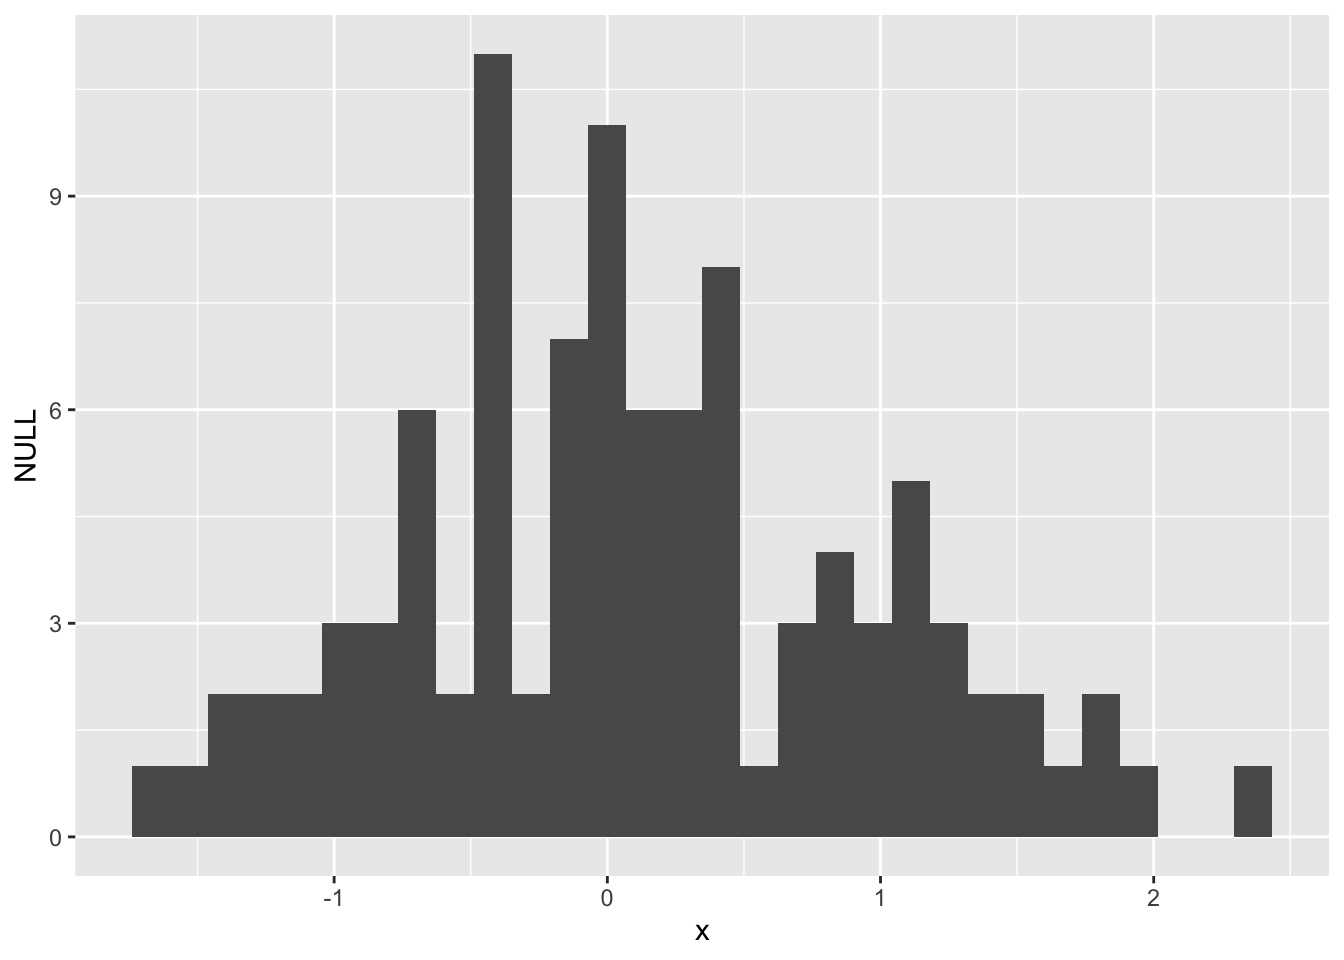
\includegraphics{Walker-elementary-statistical-modeling-draft_files/figure-latex/simple-plot-1.pdf}

\subsection{Create more R chunks and explore options and play with R
code}\label{create-more-r-chunks-and-explore-options-and-play-with-r-code}

\chapter{Data -- Importing and Saving
Data}\label{data-importing-and-saving-data}

\section{Create new notebook for this
chapter}\label{create-new-notebook-for-this-chapter}

Be sure to save the notebook in the ``notebooks'' folder of your
BIO\_413 project. Annotate your notebook with notes! Update it as you
learn more! We will use data.table for importing text files in
tab-delimited or comma-separated formats and the readxl package for
importing excel files.

Start your notebook with a chunk named ``setup''. It is important that
``setup'' is the name. The text inside the curly brackets at the top of
the chunk should be ``r setup, message=FALSE''

\begin{Shaded}
\begin{Highlighting}[]
\NormalTok{knitr}\OperatorTok{::}\NormalTok{opts_chunk}\OperatorTok{$}\KeywordTok{set}\NormalTok{(}\DataTypeTok{fig.width=}\DecValTok{6}\NormalTok{, }\DataTypeTok{fig.height=}\DecValTok{4}\NormalTok{) }

\CommentTok{# use this in a chuck called "setup" to force the working directory to be}
\CommentTok{# at the level of the project file.}
\NormalTok{knitr}\OperatorTok{::}\NormalTok{opts_knit}\OperatorTok{$}\KeywordTok{set}\NormalTok{(}\DataTypeTok{root.dir =}\NormalTok{ rprojroot}\OperatorTok{::}\KeywordTok{find_rstudio_root_file}\NormalTok{())}

\CommentTok{# relative paths to project folders}
\NormalTok{data_path <-}\StringTok{ "data"} \CommentTok{# path to data that are imported}
\NormalTok{output_path <-}\StringTok{ "output"} \CommentTok{# path to data that are saved}
\end{Highlighting}
\end{Shaded}

Add a ``load-packages'' chunk.

\begin{Shaded}
\begin{Highlighting}[]
\KeywordTok{library}\NormalTok{(ggplot2) }\CommentTok{# ggplot environment}
\KeywordTok{library}\NormalTok{(ggpubr) }\CommentTok{# publication ready plots}
\KeywordTok{library}\NormalTok{(data.table) }\CommentTok{# make data.frames data.tables}
\KeywordTok{library}\NormalTok{(readxl) }\CommentTok{# import excel}
\KeywordTok{library}\NormalTok{(emmeans) }\CommentTok{# get estimated marginal means and CIs, used for plot}
\KeywordTok{library}\NormalTok{(janitor) }\CommentTok{# clean_names to clean col labels of imported data}
\end{Highlighting}
\end{Shaded}

\section{Importing Data}\label{importing-data}

Throughout this book, we will download data from the
\href{https://datadryad.org}{Dryad Digital Repository}, which is a major
resource for increasing reproducibility in science. My own view is that
\emph{all data} should be archived on some public server (exceptions
include data that are proprietary or contain sensitive information --
such as human health measures).

The downloaded data will be inserted into the ``data'' folder. To access
these data in an R script, the script needs to know ``where to look'' or
the ``address.'' This address is the \textbf{path}. The default
\textbf{working directory} for an R notebook is the directory containing
the notebook .Rmd file so the default path is the path to this directory
and this file should always be saved to the ``notebooks'' folder within
``BIO\_413''. The setup chunk above changes this default working
directory to the project folder, which makes it a little easier to
navigate to the data folder.

``BIO\_413'' Folder is the parent of the ``notebooks'' folder. It is
also the parent of the ``data'' folder. To see any content within the
``data'' folder, the R script needs to tell R to move back (or up) the
directory structure out of the ``notebooks'' folder into the parent
``BIO\_413'' folder and then forward (or down) into the ``data'' folder.
This would be do

\subsection{Excel File}\label{excel-file}

The Excel dataset is from an experiment on the growth response of zebra
finch chicks to an incubation call that presumably signals ``hot
environment'' to the embryos
(\href{http://science.sciencemag.org/content/353/6301/812}{Mariette,
M.M. and Buchanan, K.L., 2016. Prenatal acoustic communication programs
offspring for high posthatching temperatures in a songbird. Science,
353(6301), pp.812-814}). The source file is from the Dryad Repository
here:

\textbf{file name}: ``allDatasetsMarietteBuchanan2016.xls''

\textbf{source}: \url{https://datadryad.org//handle/10255/dryad.122315}

Steps

\begin{enumerate}
\def\labelenumi{\arabic{enumi}.}
\tightlist
\item
  Copy the title of the Dryad page, which is ``Data from: Prenatal
  acoustic communication programs offspring for high post-hatching
  temperatures in a songbird''
\item
  Create a new folder within ``data'' and paste in the copied title as
  the folder name
\item
  Remove the colon from the name, so the folder name is ``Data from
  Prenatal acoustic communication programs offspring for high
  post-hatching temperatures in a songbird''
\item
  Download the .xls file into this folder
\end{enumerate}

A .xls file is an old (pre 2007) Microsoft Excel file type. It is a
binary file and can only be opened into a readable format with
specialized software. The more modern Excel file type is .xlsx, which
contains within it multiple xml components. An xml file is a text file,
and so contains readable content, but the content is xml code to display
something. In general, I am a big advocate of archiving stuff as text
files (manuscripts, data, scripts, blog posts) because these will
\emph{always} be readable by future software. Microsoft Excel is not
likely to die anytime soon and software that can read .xls and
especially .xlsx files (again, .xlsx files are text files) is even less
likely to disappear but we can feel even more confident if data are
archived as text files. That said, a single microsoft excel file with
multiple sheets is an efficient method for distributing data and the
readxl package provides excellent tools for reading different sheets of
a single .xls or .xlsx file.

The code below uses the function \texttt{read\_excel()} from the package
readxl. More about the amazing power of this package is the
\href{https://readxl.tidyverse.org}{tidyverse page} and
\href{http://r4ds.had.co.nz/data-import.html}{chapter 11} in the \emph{R
for Data Science} book.

\begin{Shaded}
\begin{Highlighting}[]
\NormalTok{data_folder <-}\StringTok{ "Data from Prenatal acoustic communication programs offspring for high post-hatching temperatures in a songbird"}
\NormalTok{filename <-}\StringTok{ "allDatasetsMarietteBuchanan2016.xls"}
\NormalTok{file_path <-}\StringTok{ }\KeywordTok{paste}\NormalTok{(data_path, data_folder, filename, }\DataTypeTok{sep=}\StringTok{"/"}\NormalTok{)}
\NormalTok{chick <-}\StringTok{ }\KeywordTok{read_excel}\NormalTok{(file_path, }\DataTypeTok{sheet=}\StringTok{"nestlingMass"}\NormalTok{) }\CommentTok{# read the excel file}
\NormalTok{chick <-}\StringTok{ }\KeywordTok{data.table}\NormalTok{(chick) }\CommentTok{# convert to data.table}
\end{Highlighting}
\end{Shaded}

In this book, we will consistently uses this protocol for storing and
retrieving downloaded files. The first three lines in the script above
creates the directory path to the file. This path includes

\begin{enumerate}
\def\labelenumi{\arabic{enumi}.}
\tightlist
\item
  data\_path -- the relative path into the folder ``data'' (relative to
  the location of the project file)
\item
  data\_folder -- the name of the folder within ``data'' containing the
  file
\item
  filename -- the name of the file to read
\end{enumerate}

These are all put together into a single path using the function
\texttt{paste()}. Read about paste. It will be used repeatedly. The
\texttt{read\_excel(file\_path,\ sheet="nestlingMass")} reads the
nestlingMass sheet only. The next
line:\texttt{chick\ \textless{}-\ data.table(chick)} converts the
data.frame into a data.table.

\subsubsection{Troubleshooting File
Import}\label{troubleshooting-file-import}

If you get an error that starts with ``Error: \texttt{path} does not
exist:'' then R is not ``seeing'' your specified file given the path
you've given it.

\begin{enumerate}
\def\labelenumi{\arabic{enumi}.}
\tightlist
\item
  Make sure your ``setup'' chunk is called ``setup'' and that it
  includes the line to change the working directory to the project
  directory and that you have run the chunk
\item
  Make sure the path to the data folder is in your setup chunk.
\item
  Make sure your ``data'' folder is \emph{one level} inside your project
  folder. ``one level'' means it is not buried deeper inside other
  folders within the project folder.
\item
  Make sure your ``Data from \ldots{}'' folder is one level inside your
  ``data'' folder
\item
  Make sure you have the name of the ``Data from \ldots{}'' folder
  correct in your script. To do this, I do not type the name but instead
  go to the finder (on Mac OS) and highlight the ``Data from \ldots{}''
  folder and copy the name -- the whole name -- and then paste in
  between the quote mark in the line
  \texttt{data\_folder\ \textless{}-\ ""}
\item
  Make sure your data file is one level inside the correct ``Data from''
  folder.
\item
  Make sure the file name is correct in the script. As with the folder
  name, I go to the finder and copy the file name and paste it in place.
\end{enumerate}

More generally, R is \emph{very literal} when it comes to: Spelling.
Humans are very good at understanding misspelled words but the R
language (or any computer language) is very literal. ``Data from
Quantifying the effects of'' and ``Data from Quantifying the efects of''
are different values. Capitalization. R is \textbf{case sensitive} (some
programming languages are not). ``Data from Quantifying'', ``Data from
quantifying'', and ``data from quantifying'' are all different values.
Spelling AND capitalization have to be perfect, not simply close. Humans
are very good at understanding misspelled and OdDLy capitalized words
but the R language (or any computer language) is very literal.

\subsubsection{Peak at the imported data.table to check that the file
was imported correctly and to learn about the
contents.}\label{peak-at-the-imported-data.table-to-check-that-the-file-was-imported-correctly-and-to-learn-about-the-contents.}

Insert the following after your import script and run:

\begin{Shaded}
\begin{Highlighting}[]
\KeywordTok{head}\NormalTok{(chick) }\CommentTok{# check -- are there headers? are there the correct number of columns?}
\end{Highlighting}
\end{Shaded}

\begin{verbatim}
##       chick ID brood ID brood composition sex rank in nest
## 1:    N1.10LF3  N1.10m3             mixed   F            2
## 2: N1.10noCut3  N1.10m3             mixed   M            4
## 3:    N1.10RB3  N1.10m3             mixed   F            2
## 4:    N1.10RF3  N1.10m3             mixed   F            5
## 5:    N1.12LB3  N1.12m3             mixed   F            3
## 6:    N1.12LF3  N1.12m3             mixed   F            1
##    playback treatment nest temperature above ambient
## 1:              treat                       4.289583
## 2:               cont                       4.289583
## 3:               cont                       4.289583
## 4:               cont                       4.289583
## 5:               cont                       3.972917
## 6:              treat                       3.972917
##    max daily temp hatch day mean max temp hatch to day2
## 1:                     17.4                    18.83333
## 2:                     19.0                    20.53333
## 3:                     17.4                    18.83333
## 4:                     19.0                    20.53333
## 5:                     29.0                    24.63333
## 6:                     25.1                    24.80000
##    mean max temp hatch to day10 mean max temp hatch to day13 hatching mass
## 1:                        22.70                     23.05714           0.7
## 2:                        24.53                     23.41429           0.6
## 3:                        22.70                     23.05714           0.7
## 4:                        24.53                     23.41429           0.6
## 5:                        22.85                     22.91429           0.7
## 6:                        23.35                     23.24286           0.6
##              day1 mass           day2 mass         day10 mass day13 mass
## 1:  1.1000000000000001                 1.2                 NA        9.8
## 2: 0.80000000000000004  1.1000000000000001                 NA        9.1
## 3: 0.90000000000000002  1.3999999999999999                 NA        9.3
## 4:                 0.5 0.90000000000000002                 NA        7.7
## 5:                   1  1.3999999999999999 9.4000000000000004       10.1
## 6: 0.90000000000000002  1.3999999999999999 8.0999999999999996        9.6
##    day13 tarsus
## 1:        14.11
## 2:        12.90
## 3:        13.60
## 4:        13.06
## 5:        14.08
## 6:        13.46
\end{verbatim}

The function \texttt{head(chick)} script displays the first few lines of
the data.table \texttt{chick}. This is one way to check that the data
were imported correctly, to examine the column labels to ensure they
conform to best practices, and to simply get to know the contents of the
import file. In this case, it is easy to see that the column names have
spaces in them. Spaces in column names are bad practice because a column
name is a variable and variable names should not include spaces (is
\texttt{brood\ id} one variable or two?). The best practice is to
replace a blank with an underscore, for example \texttt{brood\_id}. Some
coders just mash words together into a single word like this
\texttt{broodid} but this should generally be avoided because the result
can be hard to read. Some coders also use Caps to designate new words
like this \texttt{BroodId}. This is easier to read than simple
concatenation but the underscore is the easiest to read.

The \texttt{janitor} package has a nice function to clean the column
names of a data frame. The default clean includes changing any uppercase
letter to lower case and replacing spaces with underscores. Many coders
like to work with all lowercase variable names to avoid having to hit
the shift key.

\begin{Shaded}
\begin{Highlighting}[]
\NormalTok{chick <-}\StringTok{ }\KeywordTok{clean_names}\NormalTok{(chick)}
\end{Highlighting}
\end{Shaded}

Importantly, \textbf{resist the temptation to change the column names in
the data file}, which reduces reproducibility. Leave original data files
original. Always increase reproducibility!

\subsubsection{Best practices for creating data
files}\label{best-practices-for-creating-data-files}

\begin{enumerate}
\def\labelenumi{\arabic{enumi}.}
\item
  \url{https://www.youtube.com/watch?time_continue=309\&v=Ry2xjTBtNFE}
  -- An excellent video introduction to best practices for organizing
  data in a spreadsheet that will subsequently be analyzed by statistics
  software.
\item
  Broman, K. W., \& Woo, K. H. (2017). Data organization in spreadsheets
  (No. e3183v1). \url{https://doi.org/10.7287/peerj.preprints.3183v1} --
  An excelllent review of best practices for organizing data in a
  spreadsheet.
\end{enumerate}

\subsubsection{Explore with plots}\label{explore-with-plots}

Just for fun, let's plot the data and reproduce Fig. 2A and B. We are
using the \texttt{qplot} function, which is from the ggplot2 package.
Two plots are made and only a subset of the rows are plotted in each (in
A, the subset in which playback\_treatment==``treat'' and, in B, the
subset in which playback\_treatment==``cont''). This book uses the
ggplot2 package extensively.

\begin{Shaded}
\begin{Highlighting}[]
\KeywordTok{qplot}\NormalTok{(}\DataTypeTok{x=}\NormalTok{nest_temperature_above_ambient, }\DataTypeTok{y=}\NormalTok{day13_mass, }\DataTypeTok{data=}\NormalTok{chick[playback_treatment}\OperatorTok{==}\StringTok{"treat"}\NormalTok{]) }\OperatorTok{+}
\StringTok{  }\KeywordTok{geom_smooth}\NormalTok{(}\DataTypeTok{method=}\StringTok{"lm"}\NormalTok{)}
\end{Highlighting}
\end{Shaded}

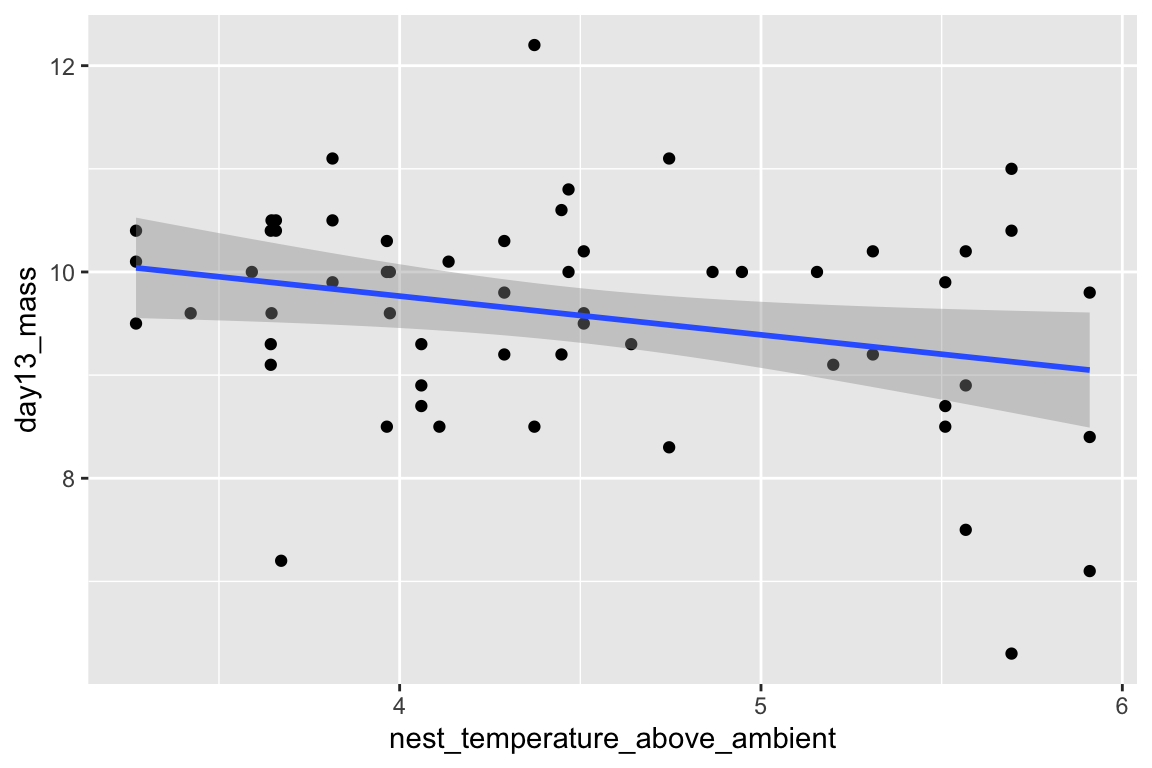
\includegraphics{Walker-elementary-statistical-modeling-draft_files/figure-latex/plotchickdata-1.pdf}

\begin{Shaded}
\begin{Highlighting}[]
\KeywordTok{qplot}\NormalTok{(}\DataTypeTok{x=}\NormalTok{nest_temperature_above_ambient, }\DataTypeTok{y=}\NormalTok{day13_mass, }\DataTypeTok{data=}\NormalTok{chick[playback_treatment}\OperatorTok{==}\StringTok{"cont"}\NormalTok{]) }\OperatorTok{+}
\StringTok{  }\KeywordTok{geom_smooth}\NormalTok{(}\DataTypeTok{method=}\StringTok{"lm"}\NormalTok{)}
\end{Highlighting}
\end{Shaded}

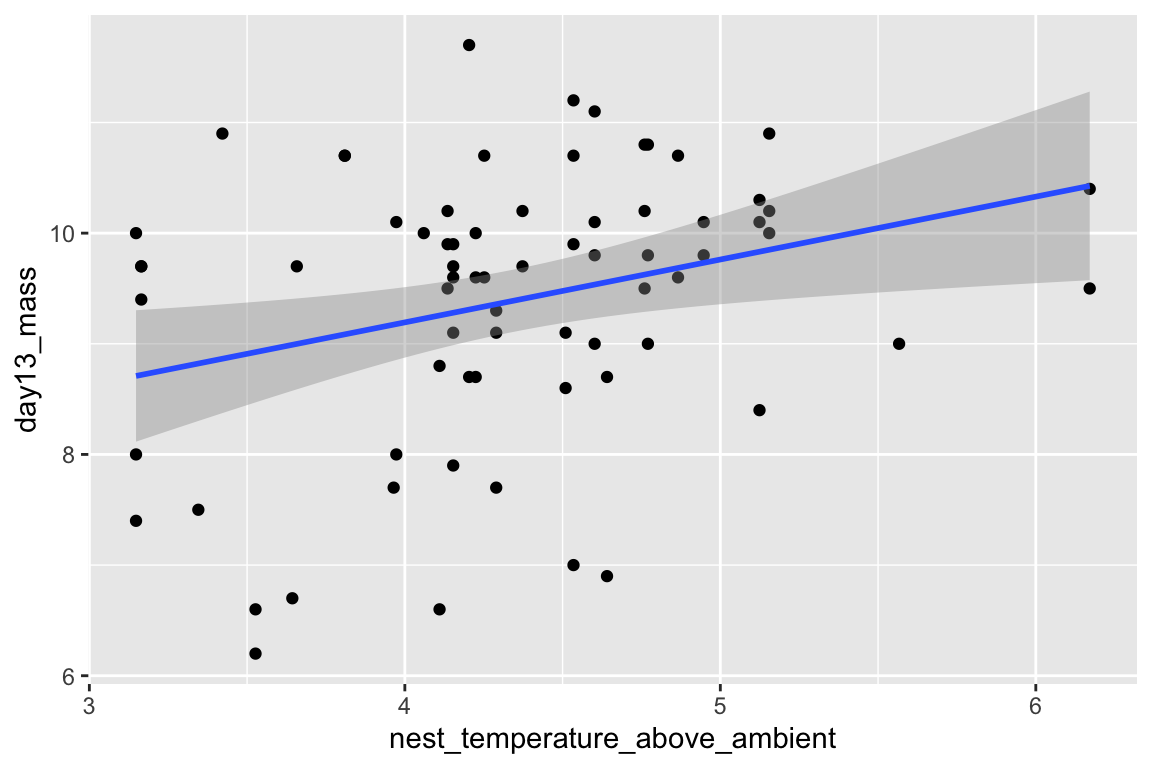
\includegraphics{Walker-elementary-statistical-modeling-draft_files/figure-latex/plotchickdata-2.pdf}

\subsection{Text File}\label{text-file}

The example dataset comes from an experiment on the effect of
\href{http://science.sciencemag.org/content/early/2012/03/28/science.1215025}{neonicotinoid
pesticides on bumble bee colony growth}.

\textbf{file name}: ``Whitehorn, O'Connor, Wackers, Goulson (2012) Data
from `Neonicotinoid pesticide reduces bumblebee colony growth and queen
production'.csv.csv''

\textbf{source}:
\url{https://datadryad.org//resource/doi:10.5061/dryad.1805c973}

Steps

\begin{enumerate}
\def\labelenumi{\arabic{enumi}.}
\tightlist
\item
  Copy the title of the Dryad page, which is ``Data from: Neonicotinoid
  pesticide reduces bumblebee colony growth and queen production''
\item
  Create a new folder within ``data'' and paste in the copied title as
  the folder name
\item
  Remove the colon from the name, so the folder name is ``Data from
  Neonicotinoid pesticide reduces bumblebee colony growth and queen
  production''
\item
  Download the .csv file into this folder
\end{enumerate}

A .csv file is a text file that is comma-delimted, which means that the
entries of a row are separated by commas. A text file is readable by any
text editor software and most other kinds of software. Datasets that are
stored as text files are typically saved as either .csv (where the
entries of a row are separated by commas) or .txt (where the entries are
separated by tabs). The base R way to read a .csv file is using
\texttt{read.csv}. The \texttt{read.table} function is more versatile,
as the delimiter can be specified. The function \texttt{fread()} from
the data.table package is fast, smart, and flexible. It is smart in the
sense that it guesses what the delimter is. Unfortunately, because of
spaces in the column labels for this file, fread guesses incorrectly
(another reason why spaces in column labels should be avoided). To
overcome this, the statement below specifies that the file contains a
``header'' (a line containing column labels)

\begin{Shaded}
\begin{Highlighting}[]
\NormalTok{data_folder <-}\StringTok{ "Data from Neonicotinoid pesticide reduces bumblebee colony growth and queen production"}
\NormalTok{filename <-}\StringTok{ "Whitehorn, O'Connor, Wackers, Goulson (2012) Data from 'Neonicotinoid pesticide reduces bumblebee colony growth and queen production'.csv.csv"}
\NormalTok{file_path <-}\StringTok{ }\KeywordTok{paste}\NormalTok{(data_path, data_folder, filename, }\DataTypeTok{sep=}\StringTok{"/"}\NormalTok{)}
\NormalTok{bee <-}\StringTok{ }\KeywordTok{fread}\NormalTok{(file_path, }\DataTypeTok{header=}\OtherTok{TRUE}\NormalTok{)}
\NormalTok{bee[, Treatment}\OperatorTok{:}\ErrorTok{=}\KeywordTok{factor}\NormalTok{(Treatment, }\KeywordTok{c}\NormalTok{(}\StringTok{"Control"}\NormalTok{, }\StringTok{"Low"}\NormalTok{, }\StringTok{"High"}\NormalTok{))]}
\KeywordTok{head}\NormalTok{(bee)}
\end{Highlighting}
\end{Shaded}

\begin{verbatim}
##    Treatment Nest ID No. workers      0      1      2   3   4    5    6
## 1:   Control      C1          13 712.95 748.30 800.57 865 966  997  850
## 2:   Control      C2          14 719.58 750.00 789.25 822 812  846  827
## 3:   Control      C3          17 704.92 736.31 767.99 837 976 1117 1050
## 4:   Control      C4          20 726.42 763.31 795.60 813 801  784   NA
## 5:   Control      C5          28 740.60 785.52 808.42 837 871  906  886
## 6:   Control      C6          15 727.10 751.90 774.80 807 847  859  827
##      7   8 V13 Workers left Males New queens Total unhatched pupae
## 1: 791 775  NA            2     0          1                    NA
## 2: 820 802  NA            6    15          0                    20
## 3: 866 808  NA            1     0          9                    NA
## 4:  NA  NA  NA            0     0          0                    12
## 5: 807 775  NA            3     0          0                    NA
## 6:  NA  NA  NA            0     0          0                   118
##    Queen pupae Empty cells
## 1:          NA          NA
## 2:           0         120
## 3:          NA          NA
## 4:           0          72
## 5:          NA          NA
## 6:          20         132
\end{verbatim}

Here, as with the import of the Excel file, the first three lines create
the directory path to the file. The treatment column is a factor
variable containing three levels (Control, Low, and High). R
automatically orders these alphabetically. For plotting and analysis, we
might want a different order. For example, we want Control to be first
in the order, since this is a natural ``reference'' level (what
everything is compared to). And if we think of ``Control'' as no
treatment, then it makes sense to have ``Low'' second in order and
``Hight'' last in order. The line
\texttt{bee{[},\ Treatment:=factor(Treatment,\ c("Control",\ "Low",\ "High")){]}}
re-orders these levels to this more meaningful order.

Again, there are spaces in the column names. \textbf{Here I'll leave it
to you to change this}

Here is a reproduction of Fig 2 from the journal article.

\begin{Shaded}
\begin{Highlighting}[]
\KeywordTok{ggbarplot}\NormalTok{(}\DataTypeTok{data=}\NormalTok{bee, }\DataTypeTok{x=}\StringTok{"Treatment"}\NormalTok{, }\DataTypeTok{y=}\StringTok{"New_queens"}\NormalTok{, }\DataTypeTok{add =} \StringTok{"mean_se"}\NormalTok{)}
\end{Highlighting}
\end{Shaded}

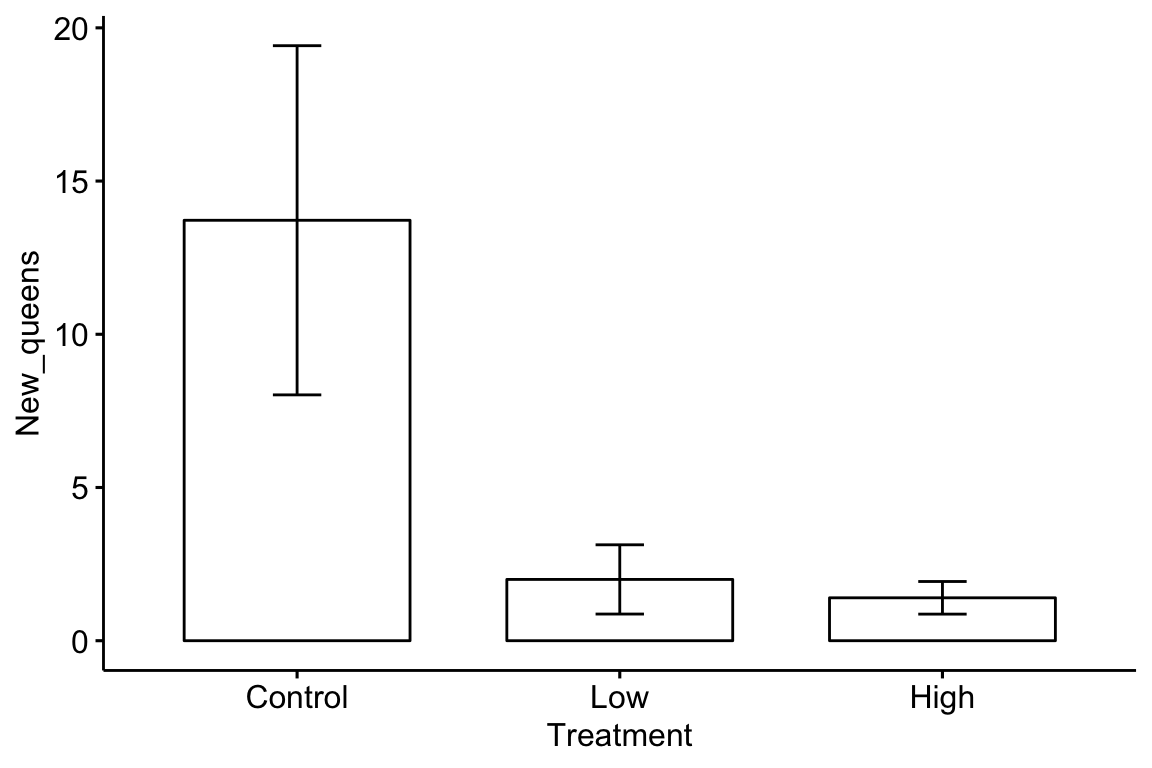
\includegraphics{Walker-elementary-statistical-modeling-draft_files/figure-latex/plot-bee-fig-2-1.pdf}

The plot suggests immediately some problems with the plot itself and the
associated analysis. First, the y-axis is counts, which means that
negative values are impossible. But the standard error bars look like
they use standard errors computed from a model that allows infinetly
large negative values, and the illustrated standard error bars imply
that negative values exist. So these error bars are misleading. Second,
it is good practice, especially if sample sizes are modest or small, to
``show the data'', which means, show the individual data points and not
just a summary of the distribution.

Here are three alternative plots for exploratory purposes. The first
simply ``shows the data'' but still uses the misleading standard error
bars. The second uses a box plot. The last plots the means and 95\%
confidence intervals modeled with a GLM (generalized linear model) to
account for the count data (the model used could be improved). Notice
that the bar length above the mean is longer than the bar length below
the mean (that is the interval is asymmetric about the mean). In order
to stay focussed on importing data, I leave explanation of these plots
and analysis to later chapters.

\begin{Shaded}
\begin{Highlighting}[]
\KeywordTok{ggbarplot}\NormalTok{(}\DataTypeTok{data=}\NormalTok{bee, }\DataTypeTok{x=}\StringTok{"Treatment"}\NormalTok{, }\DataTypeTok{y=}\StringTok{"New_queens"}\NormalTok{, }\DataTypeTok{add =} \KeywordTok{c}\NormalTok{(}\StringTok{"mean_se"}\NormalTok{, }\StringTok{"point"}\NormalTok{))}
\end{Highlighting}
\end{Shaded}

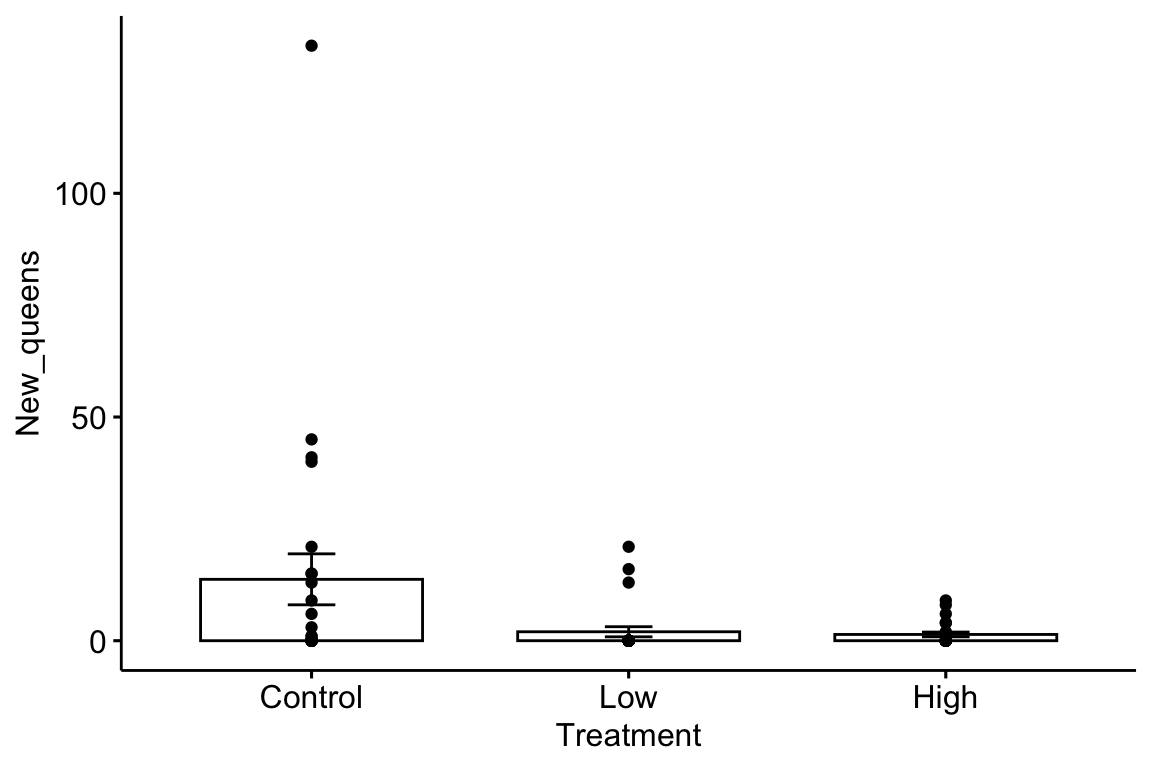
\includegraphics{Walker-elementary-statistical-modeling-draft_files/figure-latex/alternative-plots-1.pdf}

\begin{Shaded}
\begin{Highlighting}[]
\KeywordTok{ggboxplot}\NormalTok{(}\DataTypeTok{data=}\NormalTok{bee, }\DataTypeTok{x=}\StringTok{"Treatment"}\NormalTok{, }\DataTypeTok{y=}\StringTok{"New_queens"}\NormalTok{)}
\end{Highlighting}
\end{Shaded}

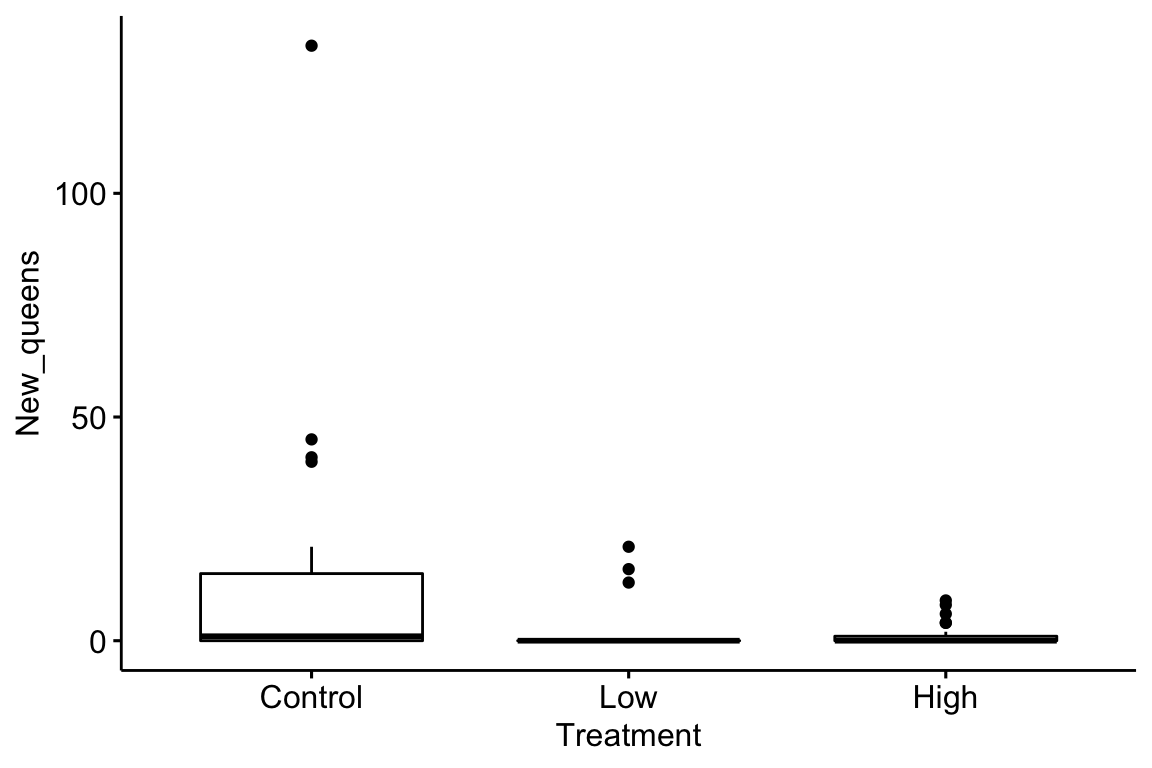
\includegraphics{Walker-elementary-statistical-modeling-draft_files/figure-latex/alternative-plots-2.pdf}

\begin{Shaded}
\begin{Highlighting}[]
\NormalTok{fit.glm <-}\StringTok{ }\KeywordTok{glm}\NormalTok{(New_queens }\OperatorTok{~}\StringTok{ }\NormalTok{Treatment, }\DataTypeTok{data=}\NormalTok{bee, }\DataTypeTok{family=}\KeywordTok{poisson}\NormalTok{())}
\NormalTok{means.glm <-}\StringTok{ }\KeywordTok{emmeans}\NormalTok{(fit.glm, }\DataTypeTok{specs=}\StringTok{"Treatment"}\NormalTok{, }\DataTypeTok{type =} \StringTok{"response"}\NormalTok{)}
\NormalTok{gg <-}\StringTok{ }\KeywordTok{ggplot}\NormalTok{(}\DataTypeTok{data=}\KeywordTok{data.frame}\NormalTok{(means.glm), }\KeywordTok{aes}\NormalTok{(}\DataTypeTok{x=}\NormalTok{Treatment, }\DataTypeTok{y=}\NormalTok{rate)) }\OperatorTok{+}
\StringTok{  }\KeywordTok{geom_col}\NormalTok{(}\DataTypeTok{fill=}\StringTok{"gray"}\NormalTok{) }\OperatorTok{+}\StringTok{ }
\StringTok{  }\KeywordTok{geom_errorbar}\NormalTok{(}\KeywordTok{aes}\NormalTok{(}\DataTypeTok{x=}\NormalTok{Treatment, }\DataTypeTok{ymin=}\NormalTok{asymp.LCL, }\DataTypeTok{ymax=}\NormalTok{asymp.UCL), }\DataTypeTok{width=}\FloatTok{0.3}\NormalTok{) }\OperatorTok{+}
\StringTok{  }\KeywordTok{ylab}\NormalTok{(}\StringTok{"New queens"}\NormalTok{) }\OperatorTok{+}
\StringTok{  }\OtherTok{NULL}
\NormalTok{gg}
\end{Highlighting}
\end{Shaded}

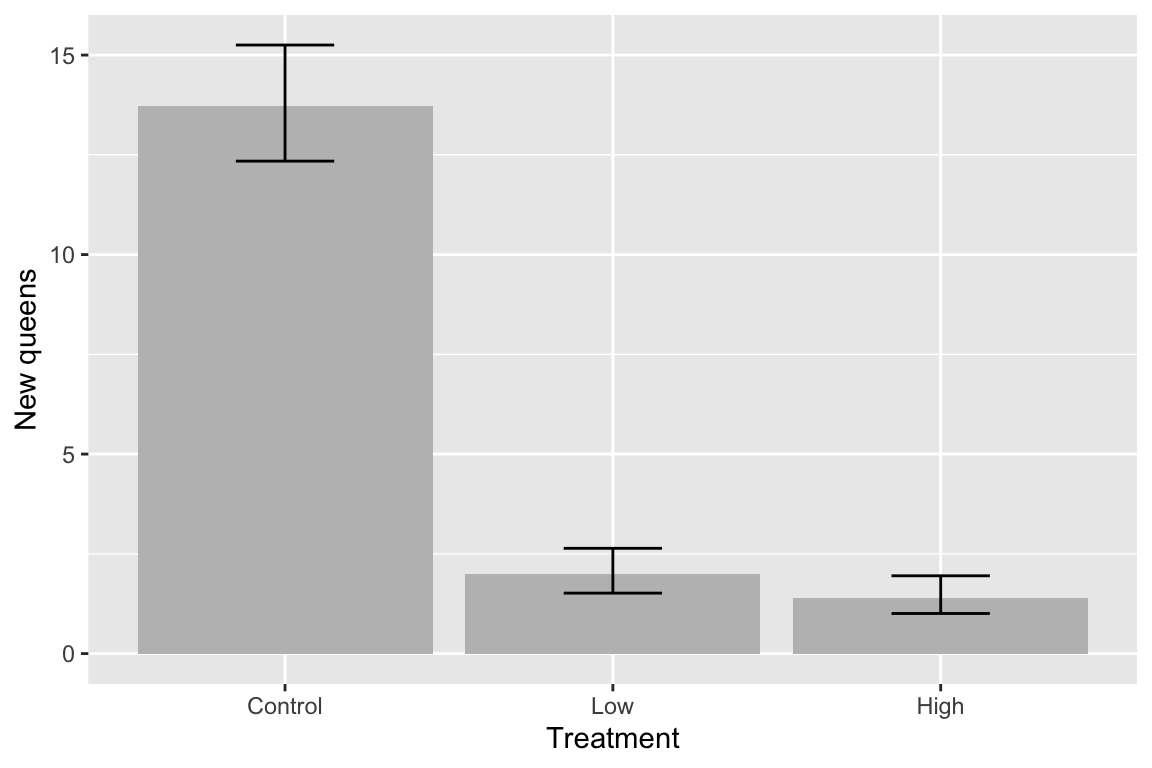
\includegraphics{Walker-elementary-statistical-modeling-draft_files/figure-latex/alternative-plots-3.pdf}

\section{Saving Data}\label{saving-data}

For many projects, it is uncommon to save data. I might save simulated
data if it takes a long time (hours or days) to generate these and I
simply want to work with the simulated data in the future (and not have
to regenerate it). Or I might save processed data if it takes a long
time to process it and I want to analyze the processed data in the
future and not have to re-process it.

Here, we will create a small, simulated data set and save it to the
``output'' folder. You should have an ``output'' folder directly
(one-level) inside the project folder. Create a folder within the output
folder names ``chapter\_02''. Make sure that you have the script
assigning the path to the output folder code in the setup chunk.

\begin{Shaded}
\begin{Highlighting}[]
\KeywordTok{set.seed}\NormalTok{(}\DecValTok{1}\NormalTok{)}
\NormalTok{n <-}\StringTok{ }\DecValTok{10}
\NormalTok{beta_}\DecValTok{0}\NormalTok{ <-}\StringTok{ }\FloatTok{10.3}
\NormalTok{beta_}\DecValTok{1}\NormalTok{ <-}\StringTok{ }\FloatTok{1.1}
\NormalTok{sigma <-}\StringTok{ }\FloatTok{1.5}
\NormalTok{fake_data <-}\StringTok{ }\KeywordTok{data.table}\NormalTok{(}\DataTypeTok{treatment=}\KeywordTok{rep}\NormalTok{(}\KeywordTok{c}\NormalTok{(}\StringTok{"Cn"}\NormalTok{,}\StringTok{"Tr"}\NormalTok{), }\DataTypeTok{each=}\NormalTok{n),}
                        \DataTypeTok{weight=}\KeywordTok{c}\NormalTok{(}\KeywordTok{rnorm}\NormalTok{(n, }\DataTypeTok{mean=}\NormalTok{beta_}\DecValTok{0}\NormalTok{, }\DataTypeTok{sd=}\NormalTok{sigma), }
                                 \KeywordTok{rnorm}\NormalTok{(n, }\DataTypeTok{mean=}\NormalTok{beta_}\DecValTok{0} \OperatorTok{+}\StringTok{ }\NormalTok{beta_}\DecValTok{1}\NormalTok{, }\DataTypeTok{sd=}\NormalTok{sigma)))}
\KeywordTok{ggstripchart}\NormalTok{(}\DataTypeTok{data=}\NormalTok{fake_data, }\DataTypeTok{x=}\StringTok{"treatment"}\NormalTok{, }\DataTypeTok{y=}\StringTok{"weight"}\NormalTok{, }\DataTypeTok{add=}\StringTok{"mean_ci"}\NormalTok{)}
\end{Highlighting}
\end{Shaded}

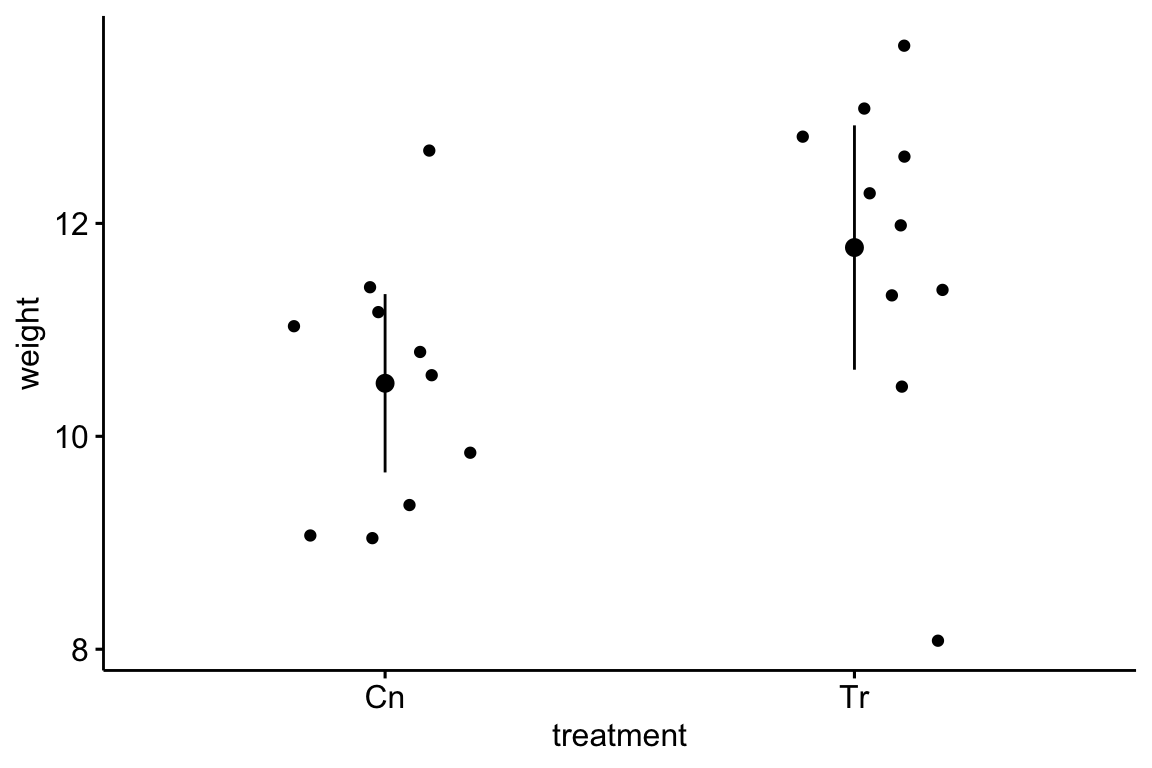
\includegraphics{Walker-elementary-statistical-modeling-draft_files/figure-latex/data-fake-data-1.pdf}

\begin{Shaded}
\begin{Highlighting}[]
\NormalTok{save_data_folder <-}\StringTok{ "chapter_02"}
\NormalTok{save_filename <-}\StringTok{ "my_first_fake_data.txt"}
\NormalTok{save_file_path <-}\StringTok{ }\KeywordTok{paste}\NormalTok{(output_path, save_data_folder, save_filename, }\DataTypeTok{sep=}\StringTok{"/"}\NormalTok{)}
\KeywordTok{write.table}\NormalTok{(fake_data, save_file_path, }\DataTypeTok{sep=}\StringTok{"}\CharTok{\textbackslash{}t}\StringTok{"}\NormalTok{, }\DataTypeTok{quote=}\OtherTok{FALSE}\NormalTok{)}
\end{Highlighting}
\end{Shaded}

Look at your project directory to make sure the file is where it should
be! We used \texttt{write.table()} to create a tab-delimited text file
using \texttt{sep="\textbackslash{}t"} to specify tabs to separate the
row elements. ``\t'' is the standard character string for a tab. Check
in your Fake\_Data folder and open the file in a text editor.

\section{Problems}\label{problems}

\begin{enumerate}
\def\labelenumi{\arabic{enumi}.}
\item
  Download the dataset ``data-Lodjak.et.al-2016-FuncEcol.xlsx'' from the
  Dryad repository at
  \url{https://datadryad.org/resource/doi:10.5061/dryad.rd01s}. The
  .xlsx file presents the data cleanly but the trade-off is that the 1)
  multiple header rows, and 2) spaces in the header labels, 3)
  parentheses in the header labels make it more complex to import in a
  usable way. Import the data and plot Body Mass against Age (that is
  make Body Mass the ``Y'' variable and Age the ``X'' variable) using
  the qplot function. You should recode the column labels to remove
  spaces and parentheses using the setnames function.
\item
  Download the dataset ``Results2015.txt'' from the Dryad repository at
  \url{https://datadryad.org//resource/doi:10.5061/dryad.65vk4}. Try to
  reproduce Fig. 1. It's not easy. I've inserted the figure below.
\item
  (grad students only) Download and plot data from a Dryad Repository
  dataset of your choice.
\item
  (grad students only) Create fake experimental data with three
  treatment levels (control, lo\_temp, high\_temp). This will require
  three parameters: an intercept (beta\_0), an effect of lo\_temp
  (beta\_1), and an effect of high\_temp (beta\_2). You should be able
  to plug and play from the script above even if you don't underdstand
  at this point what any of it is! Plot it as a strip chart, as above.
\end{enumerate}

\begin{figure}
\centering
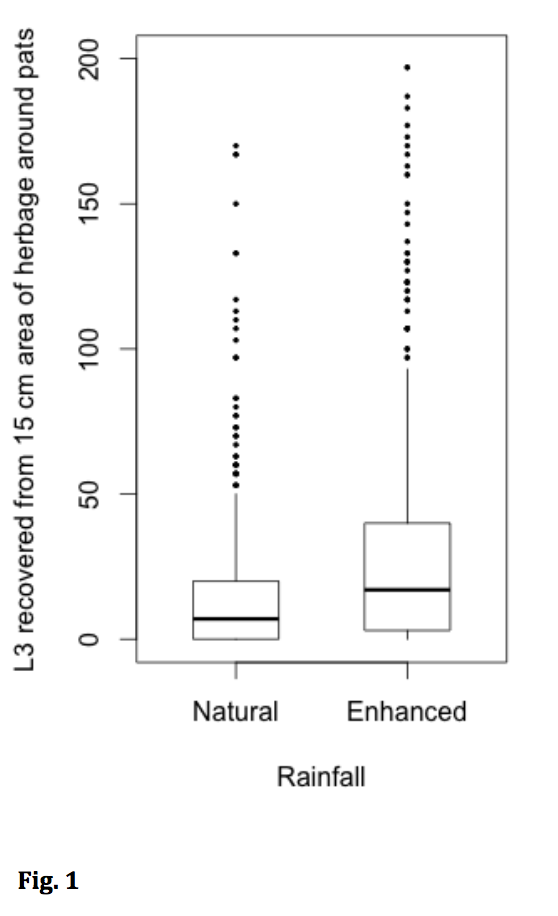
\includegraphics[width=0.50000\textwidth]{images/Dung_beetles_reduce_livestock-fig_1.png}
\caption{Fig. 1 from ``Dung beetles reduce livestock\ldots{}''}
\end{figure}

\chapter*{Part II: Some Fundamentals of Statistical
Modeling}\label{part-ii-some-fundamentals-of-statistical-modeling}
\addcontentsline{toc}{chapter}{Part II: Some Fundamentals of Statistical
Modeling}

\chapter{An Introduction to Statistical
Modeling}\label{an-introduction-to-statistical-modeling}

This chapter introduces statistical modeling using the \textbf{linear
model}. All students are familiar with the idea of a linear model from
learning the equation of a line, which is

\begin{equation}
Y = mX + b
\label{eq:line}
\end{equation}

where \(m\) is the slope of the line and \(b\) is the \(Y\)-intercept.
It is useful to think of equation \eqref{eq:line} as a function that maps
values of \(X\) to values of \(Y\). Using this function, if we input
some value of \(X\), we always get the same value of Y as the output.

A linear model is a function, like that in equation \eqref{eq:line}, that
is fit to a set of data, often to model a process that generated the
data or something like the data. The line in Figure \ref{fig:line}A is
just that, a line, but the line in Figure \ref{fig:line}B is a linear
model fit to the data in Figure \ref{fig:line}B.

\begin{figure}
\centering
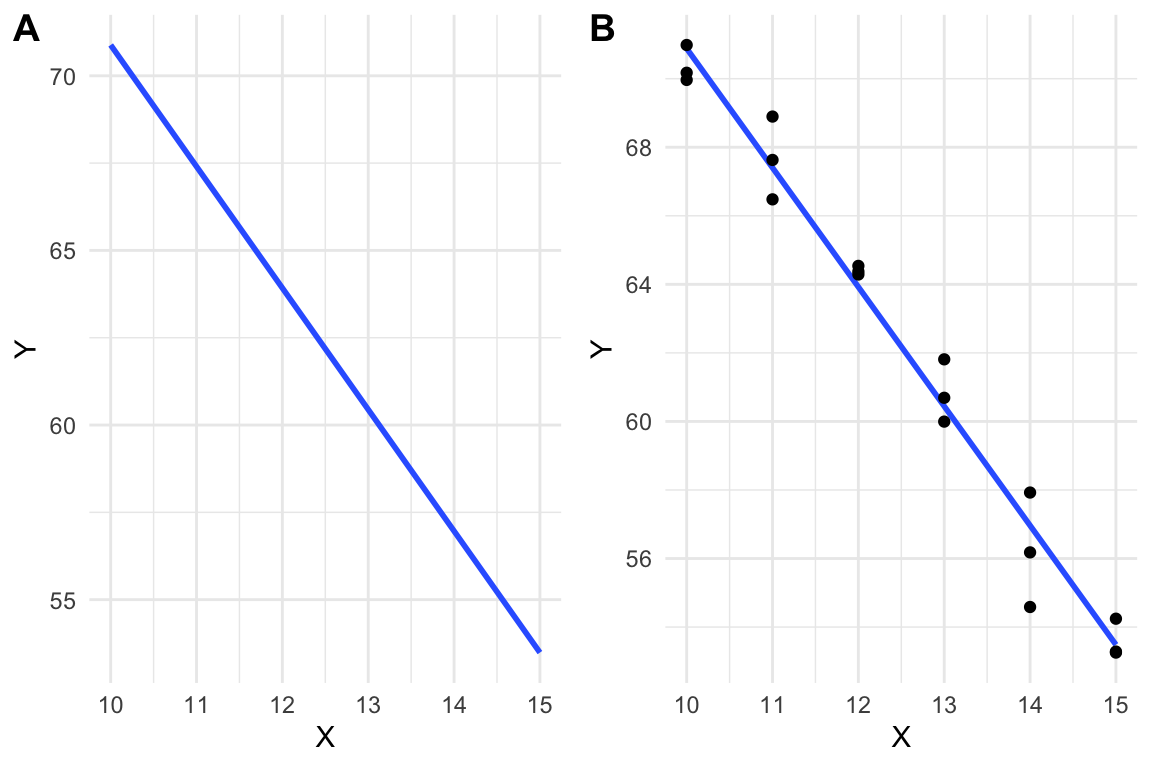
\includegraphics{Walker-elementary-statistical-modeling-draft_files/figure-latex/line-1.pdf}
\caption{\label{fig:line}A line vs.~a linear model. (A) the line
\(y=-3.48X + 105.7\) is drawn. (B) A linear model fit to the data. The
model coefficients are numerically equal to the slope and intercept of
the line in A.}
\end{figure}

\section{Two specifications of a linear
model}\label{two-specifications-of-a-linear-model}

\subsection{\texorpdfstring{The ``error draw''
specification}{The error draw specification}}\label{the-error-draw-specification}

A linear model is commonly specified using

\begin{align}
Y &= \beta_0 + \beta_1 X + \varepsilon\\
\label{eq:lm}
\end{align}

This specification of a linear model has two parts: the \textbf{linear
predictor} \(Y = \beta_0 + \beta_1 X\) and the \textbf{error}
\(\varepsilon\). The linear predictor part looks like the equation for a
line except that 1) \(\beta_0\) is used for the intercept and
\(\beta_1\) for the slope and 2) the intercept term precedes the slope
term. This re-labeling and re-arrangement make the notation for a linear
model more flexible for more complicated linear models. For example
\(Y = \beta_0 + \beta_1 X_1 + \beta_2 X_2 + \varepsilon\) is a model
where \(Y\) is a function of two \(X\) variables.

As with the equation for a line, the linear predictor part of a linear
model is a function that maps a specific value of \(X\) to a value of
\(Y\). This mapped value is the \textbf{expected value} given a specific
input value of \(X\). This is often written as \(\mathrm{E}[Y|X]\),
which is read as ``the expected value of \(Y\) given \(X\)'', where
``given X'' means a specific value of X. Importantly,
\(\mathrm{E}[Y|X]\) is the \textbf{conditional mean}, which is the
\emph{modeled} value of \(Y\) for all observations in which \(X\) takes
some specific value \(x\).

Introductory textbooks almost always introduce linear models using
equation \eqref{eq:lm} above. The key part of the model that is missing
from the specification above is a second line

\begin{equation}
\varepsilon \sim N(0, \sigma^2)
\end{equation}

which is read as ``epsilon is distributed as Normal with mean zero and
variance sigma squared''. This line explicitly specifies the
distribution of the error part. The error part of a linear model is a
random ``draw'' from a normal distribution with mean zero and variance
\(\sigma^2\). Think of this as adding some random value to the expected
value.

\subsection{\texorpdfstring{The ``conditional draw''
specification}{The conditional draw specification}}\label{the-conditional-draw-specification}

A second way of specifying a linear model is

\begin{align}
y_i &\sim N(\mu_i, \sigma^2)\\
\mathrm{E}(Y|X) &= \mu\\
\mu_i &= \beta_0 + \beta_1 x_i
\label{eq:lm-spec2}
\end{align}

The first line states that the response variable \(Y\) is a random
variable independently drawn from a normal distribution with mean
\(\mu\) and variance \(\sigma^2\). This first line is the
\textbf{stochastic} part of the statistical model. The second line
simply states that \(\mu\) (the greek letter ``mu'') from the first line
is the conditional mean or conditional expectation. The third line
states how \(\mu_i\) is generated given that \(X=x_i\). This is the
linear predictor, which is the \textbf{systematic} (or deterministic)
part of the statistical model. It is systematic because the same value
of \(x_i\) will always generate the same \(\mu_i\).

\subsection{Comparing the two ways of specifying the linear
model}\label{comparing-the-two-ways-of-specifying-the-linear-model}

These two ways of specifying the model encourage slightly different ways
of thinking about how the data (the response varible \(Y\)) were
generated. The error draw specification ``generates'' data by randomly
drawing some error \(\varepsilon_i\) from the specified distribution and
adding this to \(x_i\). The conditional draw specification ``generates''
data by constructing what \(y_i\) ``should be'' given \(x_i\) (the
conditional expection), and then drawing a random variable from a
distribution with this expectation. This random draw is \(y_i\) and not
the ``error''. For the error draw generation, we need only one hat of
random numbers, but for the conditional draw generation, we need a hat
for each value of \(x_i\).

The conditional draw specification explicitly defines all parameters,
including the parameters of the linear predictor (\(\beta_0\) and
\(\beta_1\)), the conditional mean \(\mu\) and the variance
\(\sigma^2\). The error draw specification only defines the parameters
of the linear predictor, and often these are referrred to as ``the
parameters'' in the sense that there are not other parameters. The error
draw specification is most useful for thinking about model checking a
fit linear model. The random draw specification is more generally useful
in that it is easily generalized to more complex models, including
hierarchical models, generalized linear models, and Bayesian models. In
fact, \emph{thinking about a model as a predictor plus error can lead to
the misconception that in a generalized linear models, the error has the
distribution (binomial, poisson, etc.) modeled}.

Although a linear model (or statistical model more generally) is a model
of a data-generating process, linear models are not typically used to
actually generate any data. Instead, when we use a linear model to
understand something about a real dataset, we think of our data as one
realization of a process that generates data like ours. A linear model
is a model of that process. That said, it is incredibly useful to use
linear models to create fake datasets for at least two reasons: to probe
our understanding of statistical modeling generally and, more
specifically, to check that a model actually creates data like that in
the real dataset that we are analyzing.

\section{\texorpdfstring{What do we call the \(X\) and \(Y\)
variables?}{What do we call the X and Y variables?}}\label{what-do-we-call-the-x-and-y-variables}

The inputs to a linear model (the \(X\) variables) have many names
including ``independent variables,'' ``predictor variables,'',
``explanatory variables,'' ``treatment variables,'' and ``covariates''.
The output of a linear model (the \(Y\) variable or variables if the
model is multivariate) is the ``dependent variable,'' ``response,'' or
``outcome.'' The \(\beta\) in the linear model are model
\textbf{parameters} and if a parameter is multiplied by an \(X\)
variable then it is also a \textbf{coefficient} (for example,
\(\beta_1\) in model \eqref{eq:lm} is a coefficient). The coefficients of
the \(X\) in a linear model (\(\beta_1\) in model \eqref{eq:lm}) are often
called ``the effects'' (so \(\beta_1\) is the effect of \(X_1\)).

\section{Statistical models are used for prediction, explanation, and
description}\label{statistical-models-are-used-for-prediction-explanation-and-description}

Researchers typically use statistical models to understand relationships
between one or more \(Y\) variables and one or more \(X\) variables.
These relationships include

\begin{enumerate}
\def\labelenumi{\arabic{enumi}.}
\item
  Descriptive modeling. Sometimes a researcher merely wants to describe
  the relationship between \(Y\) and a set of \(X\) variables, perhaps
  to discover patterns. For example, the arrival of a spring migrant
  bird (\(Y\)) as a function of sex (\(X_1\)) and age (\(X_2\)) might
  show that males and younger individuals arrive earlier. Importantly,
  if another \(X\) variable is added to the model (or one dropped), the
  coefficients, and therefore, the precise description, will change.
  That is, the interpretation of a coefficient as a descriptor is
  \emph{conditional} on the other covariates (\(X\) variables) in the
  model. In a descriptive model, there is no implication of causal
  effects and the goal is not prediction. Nevertheless, it is very hard
  for humans to discuss a descriptive model without using causal
  language, which probably means that it is hard for us to think of
  these models as \emph{mere description}. Like natural history,
  descriptive models are useful as patterns in want of an explanation,
  using more explicit causal models including experiments.
\item
  Predictive modeling. Predictive modeling is very common in applied
  research. For example, fisheries researchers might model the
  relationship between population density and habitat variables to
  predict which subset of ponds in a region are most suitable for brook
  trout (\emph{Salvelinus fontinalis}) reintroduction. The goal is to
  build a model with minimal prediction error, which is the error
  between predicted and actual values for a future sample. In predictive
  modeling, the \(X\) (``predictor'') variables are largely instrumental
  -- how these are related to \(Y\) is not a goal of the modeling,
  although sometimes an investigator may be interested in the relative
  importance among the \(X\) for predicting \(Y\) (for example,
  collecting the data may be time consuming, or expensive, or
  enviromentally destructive, so know which subset of \(X\) are most
  important for predicting \(Y\) is a useful strategy).
\item
  Explanatory (causal) modeling. Very often, researchers are explicitly
  interested in \emph{how} the \(X\) variables are causally related to
  \(Y\). The fisheries researchers that want to reintroduce trout may
  want to develop and manage a set of ponds to maintain healthy trout
  populations. This active management requires intervention to change
  habitat traits in a direction, and with a magnitude, to cause the
  desired response. This model is predictive -- a specific change in
  \(X\) predicts a specific response in \(Y\) -- because the
  coefficients of the model provide knowledge on how the system
  functions -- how changes in the inputs \emph{cause} change in the
  output. Causal interpretation of model coefficients requires a set of
  strong assumptions about the \(X\) variables in the model. These
  assumptions are typically met in \textbf{experimental designs} but not
  \textbf{observational designs}.
\end{enumerate}

With observational designs, biologists are often not very explicit about
which of these is the goal of the modeling and use a combination of
descriptive, predictive, and causal language to describe and discuss
results. Many papers read as if the researchers intend explanatory
inference but because of norms within the biology community, mask this
intention with ``predictive'' language. Here, I advocate embracing
explicit, explanatory modeling by being very transparent about the
model's goal and assumptions.

\section{Modeling strategy}\label{modeling-strategy}

\begin{enumerate}
\def\labelenumi{\arabic{enumi}.}
\item
  \textbf{choose a model}. Statistical modeling includes a diverse array
  of models, yet almost all methods used by researchers in biology, and
  all models in this book, are generalizations of the linear model
  specified in \ref{eq:}.
\item
  \textbf{fit the model}, in order to estimate the model parameters and
  the uncertainty in these estimates.
\item
  \textbf{check the model}, which means to use a series of diagnostic
  plots and computations of model output to check that the data
  reasonably approximate the chosen model.
\item
  \textbf{inference from the model}, which means to use the fit
  parameters to learn, with uncertainty, about the system, or to predict
  future observations, with uncertainty.
\item
  \textbf{plot the model}, which means to plot the estimated parameters
  (or other results dervived from the estimates) with their uncertainty.
\end{enumerate}

In order to use a statistical model to describe, predict, or explain, we
need to fit a model to data in order to estimate the parameters. A
linear model fit to some data is

\begin{align}
\hat{y}_i &= b_0 + b_1 x_i + e_i\\
\label{eq:yhat}
\end{align}

\(\hat{y}_i\) (``y hat'') is the \textbf{predicted value} of individual
\(i\), \(b_0\) and \(b_1\) are the coefficients of the model fit (though
technically \(b_0\) is not a coefficient), and \(e_i\) is the residual.
Sometimes \(\hat{y}_i\) is simply called ``the prediction''.

If our goal is inference -- to infer something about the ``population''
from the sample using the fit model, then \(\hat{y}_i\) is the
\textbf{point estimate} of the parameter \(\mu_i\), the coefficients
\(b_0\) and \(b_1\) are point estimates of the parameters \(\beta_0\)
and \(\beta_1\), and the standard deviation of the \(e_i\) is an
estimate of \(\sigma\). ``Population'' is in quotes because it is a very
abstract concept. Throughout this book, Greek letters refer to a
theoretical parameter and Roman letters refer to point estimates.

Throughout this text, I recommend reporting and interpreting
\textbf{interval estimates} of the point estimate. A \textbf{confidence
interval} is a type of interval estimate. A confidence interval of a
parameter is a measure of the uncertainty in the estimate. A 95\%
confidence interval has a 95\% probability (in the sense of long-run
frequency) of containing the parameter This probability is a property of
the population of intervals that could be computed using the same
sampling and measuring procedure. It is not correct, without further
assumptions, to state that there is a 95\% probability that the
parameter lies within the interval. Perhaps a more useful interpretation
is that the interval is a \textbf{compatability interval} in that it
contains the range of estimates that are compatible with the data, in
the sense that a \(t\)-test would not reject the null hypothesis of a
difference between the estimate and any value within the interval (this
interpretation does not imply anything about the true value).

\begin{figure}
\centering
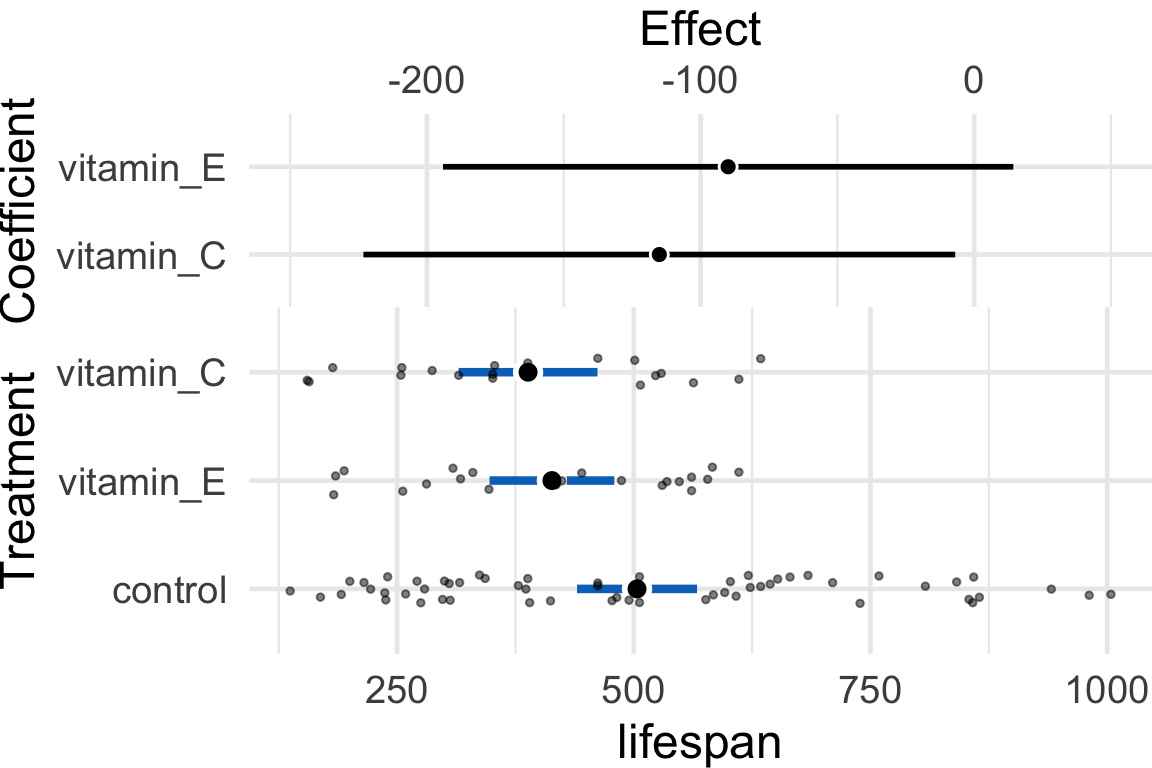
\includegraphics{Walker-elementary-statistical-modeling-draft_files/figure-latex/coldVoles-1.pdf}
\caption{\label{fig:coldVoles}HarrellPlot of vole data.}
\end{figure}

For the model fit to the data in Figure \ref{fig:line}B, the coefficient
of \(X\) is the slope of the line. Perhaps surprisingly, we can fit a
model like equation \eqref{eq:lm} to data in which the \(X\) variable is
categorical. A simple example is the experiment of antioxidants
(vitamins C and E) on lifespan in Voles (Fig. \ref{fig:coldVoles}). In
this experiment, the \(X\) variable is categorical, with three
\textbf{levels}: ``Control'', ``Vitamin\_E'' and ``Vitamin\_C''.
Categorical \(X\) variables are often called \textbf{factors}. The trick
to using a statistical model with categorical \(X\) is to recode the
factor levels into numbers -- how this is done is explained in Chapter
xxx. When the \(X\) variable is categorical, the coefficients of the
\(X\) are \emph{differences in group means}. The linear model fit to the
vole data has two coefficients, one for Vitamin E and one for vitamin C.
The estimate and uncertainty of the these two coefficients are shown in
the top part of Figure \ref{fig:coldVoles}. The bottom part shows the
raw data, as well as the group (factor level) means and the uncertainty
in the estimate of these means.

\section{A mean is the simplest
model}\label{a-mean-is-the-simplest-model}

The simplest possible model that can be fit to the data is

\begin{equation}
\mathrm{E}[Y] = b_0
\label{eq:unconditional}
\end{equation}

which is simply the mean of \(Y\), or, more specifically, the
\textbf{unconditional mean} of \(Y\), since its value is not conditional
on any value of \(X\).

\section{Assumptions for inference with a statistical
model}\label{assumptions-for-inference-with-a-statistical-model}

\textbf{Inference} refers to using the fit model to generalize from the
sample to the population, which assumes that the response is drawn from
some specified probability distribution (Normal, or Poisson, or
Bernouli, etc.). Throughout this text, I emphasize reporting and
interpreting point estimates and confidence intervals. Another kind of
inference is a \textbf{significance test}, which is the computation of
the probability of ``seeing the data'' or something more extreme than
the data, given a specified null hypothesis. A significance test results
in a \textbf{p-value}, which can be reported with the point estimate and
confidence interval. Somewhat related to a significance test is a
hypothesis test, or what is now often perjoratively called a
\textbf{Null-Hypothesis Signficance Test} (NHST), in which the
\(p\)-value from a significance test is compared to a pre-specified
error rate called \(\alpha\). NHST may be useful for some very limited
kinds of science but, in general, is not useful for most biological
research and, instead, leads to large misconceptions. A general rule of
thumb is, do not compare a reported \(p\)-value to \(\alpha\).

\begin{enumerate}
\def\labelenumi{\arabic{enumi}.}
\tightlist
\item
  The data were generated by a process that is ``linear in the
  parameters'', which means that the different components of the model
  are added together. This additive part of the model containing the
  parameters is the linear predictor in specifications \eqref{eq:lm} and
  \eqref{eq:lm-spec2} above. For example, a cubic polynomial model
\end{enumerate}

\begin{equation}
\mathrm{E}(Y|X) = \beta_0 + \beta_1 X + \beta_2 X^2 + \beta_3 X^3
\end{equation}

is a linear model, even though the function is non-linear, because the
different components are added. Because a linear predictor is additive,
it can be compactly defined using matrix algebra

\begin{equation}
\mathrm{E}(Y|X) = \mathbf{X}\boldsymbol{\beta}
\end{equation}

where \(mathbf{X}\) is the \textbf{model matrix} and
\(\boldsymbol{\beta}\) is the vector of parameters. We discuss these
more in chapter xxx.

A \textbf{Generalized Linear Model} (GLM) has the form
\(g(\mu_i) = \eta_i\) where \(\eta\) (the Greek letter ``eta'') is the
linear predictor

\begin{equation}
\eta = \mathbf{X}\boldsymbol{\beta} 
\end{equation}

GLMs are extensions of linear models. There are non-linear models that
are not linear in the parameters, that is, the predictor is not a simple
dot product of the model matrix and a vector of parameters. For example,
the Michaelis-Menten model is a non-linear model

\begin{equation}
\mathrm{E}(Y|X)  = \frac{\beta_1 X}{\beta_2 + X}
\end{equation}

that is non-linear in the parameters because the parts are not added
together. This text covers linear models and generalized linear models,
but not non-linear models that are also non-linear in the parameters.

\begin{enumerate}
\def\labelenumi{\arabic{enumi}.}
\setcounter{enumi}{1}
\tightlist
\item
  The draws from the probability distribution are \textbf{independent}.
  Independence implies \textbf{uncorrelated} observations (the \(Y\)),
  that is, for any two observations with the same value of \(X\), we
  cannot predict the value of one given the value of the other. For
  example, in the vole data above, uncorrelated implies that we cannot
  predict the lifespan of one vole within the Vitamin E treatment given
  the lifespan of another vole in the Vitamin E treatment. For linear
  models, this assumption is often stated as ``independent errors'' (the
  \(\varepsilon\) in model \eqref{eq:lm}) instead of independent
  observations.
\end{enumerate}

There are lots of reasons that observations might be correlated. In the
vole example, perhaps the voles were housed in batches of 5 individuals,
and slight differences in the environment among the housing containers,
caused all the voles in some containers to have shorter lifespans than
expected given their treatment assigment and all voles in other
containers to have longer lifespans than expected given their treatment
assigment. More generally, if there are measures both within and among
experimental units (field sites or humans or rats) then we'd expect the
measures within the same unit to err from the model in the same
direction. Multiple measures within experimental units (a site or
individual) creates ``clustered'' observations. Lack of independence or
clustered observations can be modeled using models with \textbf{random
effects}. These models go by many names including linear mixed models
(common in Ecology), hierarchical models, multilevel models, and random
effects models. A linear mixed model is a variation of model
\eqref{eq:lm}. This text introduces linear mixed models in chapter xxx.

Measures that are taken from sites that are closer together or measures
taken closer in time or measures from more closely related biological
species will tend to have more similar values than measures taken from
sites that are further apart or from times that are further apart or
from species that are less closely related. Space and time and phylogeny
create \textbf{spatial and temporal and phylogenetic autocorrelation}.
Correlated error due to space or time or phylogeny can be modeled with
\textbf{Generalized Least Squares} (GLS) models. A GLS model is a
variation of model \eqref{eq:lm}.

\section{Specific assumptions for inference with a linear
model}\label{specific-assumptions-for-inference-with-a-linear-model}

\begin{enumerate}
\def\labelenumi{\arabic{enumi}.}
\tightlist
\item
  \textbf{Constant variance} or \textbf{homoskedasticity}. The most
  common way of thinking about this is the error term \(\varepsilon\)
  has constant variance, which is a short way of saying that random
  draws of \(\varepsilon\) in model \eqref{eq:lm} are all from the same
  (or \textbf{identical}) distribution. This is explicitly stated in the
  second line of model specification \eqref{eq:lm}. If we were to think
  about this using model specification \eqref{eq:lm-spec2}, then
  homoskedasticity means that \(\sigma\) in \(N(\mu, \sigma)\) is
  constant for all observations (or that the \emph{conditional}
  probability distributions are identical, where \emph{conditional}
  would mean adjusted for \(\mu\))
\end{enumerate}

Many biological processes generate data in which the error is a function
of the mean. For example, measures of biological variables that grow,
such as lengths of body parts or population size, have variances that
``grow'' with the mean. Or, measures of counts, such as the number of
cells damaged by toxin, the number of eggs in a nest, or the number of
mRNA transcripts per cell have variances that are a function of the
mean. Heteroskedastic error can be modeled with \textbf{Generalized
Least Squares}, a generalization of the linear model, and with
\textbf{Generalized Linear Models} (GLM), which are ``extensions'' of
the classical linear model.

\begin{enumerate}
\def\labelenumi{\arabic{enumi}.}
\setcounter{enumi}{1}
\tightlist
\item
  Normal or \textbf{Gaussian} probability distribution. As above, the
  most common way of thinking about this is the error term
  \(\varepsilon\) is Normal. Using model specification
  \eqref{eq:lm-spec2}, we'd say the conditional probablity distribution of
  the response is normal. A normal probability distribution implies that
  1) the response is continuous and 2) the conditional probability is
  symmetric around \(mu_i\). If the conditional probability distribution
  has a long left or right tail it is \textbf{skewed} left or right.
  Counts (number of cells, number of eggs, number of mRNA transcripts)
  and binary responses (sucessful escape or sucessful infestation of
  host) are not continuous and often often have asymmetric probablity
  distributions that are skewed to the right and while sometimes both
  can be reasonably modeled using a linear model they are more often
  modeled using generalized linear models, which, again, is an extension
  of the linear model in equation \eqref{eq:lm-lm-spec2}.
\end{enumerate}

A common misconception is that inference from a linear model assumes
that the \emph{response} (\(Y\)) is normally distributed. Both the
``linear model'' and ``statistical model'' ways of specifying the model
show precisely why this conception is wrong. Model \eqref{eq:lm} states
explicitly that it is the error that has the normal distribution -- the
distribution of \(Y\) is a mix of the distribution of \(X\) and the
error. Model \eqref{eq:lm-spec2} states that the conditional outcome has a
normal distribution, that is, the distribution after adjusting for
variation in \(X\).

\section{\texorpdfstring{``Statistical model'' or ``regression
model''?}{Statistical model or regression model?}}\label{statistical-model-or-regression-model}

Statistical modeling terminology can be confusing. The \(X\) variables
in a statistical model may be quantitative (continuous or integers) or
categorical (names or qualitative amounts) or some mix of the two.
Linear models with all quantitative independent variables are often
called ``regression models.'' Linear models with all categorical
independent variables are often called ``ANOVA models.'' Linear models
with a mix of quantitative and categorical variables are often called
``ANCOVA models'' if the focus is on one of the categorical \(X\) or
``regression models'' if there tend to be many independent variables.
Other patterns occur. For example ``ANCOVA models'' often include
interaction effects but ``regression models'' rarely do. To avoid
thinking of statistical analysis as ``regression vs.~ANOVA'' (the type
of thinking encouraged by many textbooks in biostatistics), I will most
often use the term ``statistical model'' for general usage, and use a
more specific term only to emphasize something about the model in that
particluar context.

\section{GLM vs.~GLM vs.~GLS}\label{glm-vs.glm-vs.gls}

Linear models are sometimes called ``general linear models'' with the
abbreviation GLM. This is unfortunate because the abbreviation GLM
usually refers to \textbf{generalized linear models}. Regardless, don't
confuse either version of GLM with GLS, which is the abbreviation of
\textbf{generalized least squares}. GLS generalizes the linear model to
allow for heteroskedastic and/or correlated error (using the ``linear
model'' way of thinking about model specification)

\chapter{Variability and Uncertainty (Standard Deviations, Standard
Errors, Confidence
Intervals)}\label{variability-and-uncertainty-standard-deviations-standard-errors-confidence-intervals}

\textbf{Uncertainty} is the stuff of science. A major goal of statistics
is measuring uncertainty. What do we mean by uncertainty? Uncertainty is
the error in estimating a parameter, such as the mean of a sample, or
the difference in means between two experimental treatments, or the
predicted response given a certain change in conditions. Uncertainty is
measured with a \textbf{variance} or its square root, which is a
\textbf{standard deviation}. The standard deviation of a statistic is
also (and more commonly) called a \textbf{standard error}.

Uncertainty emerges because of variability. In any introductory
statistics class, students are introduced to two measures of
variability, the ``standard deviation'' and the ``standard error.''
These terms are absolutely fundamental to statistics -- they are the
start of everything else. Yet, many biology researchers confuse these
terms and certainly, introductory students do too.

When a research biologist uses the term ``standard deviation,'' they are
probably referring to the sample standard deviation which is a measure
of the variability of a sample. When a research biologist uses the term
``standard error,'' they are probably referring to the standard error of
a mean, but it could be the standard error of another statistics, such
as a difference between means or a regression slope. An important point
to remember and understand is that all standard errors \emph{are}
standard deviations. This will make more sense soon.

\section{The sample standard deviation vs.~the standard error of the
mean}\label{the-sample-standard-deviation-vs.the-standard-error-of-the-mean}

\subsection{Sample standard deviation}\label{sample-standard-deviation}

The sample standard deviation is a measure of the variability of a
sample. For example, were we to look at a histological section of
skeletal muscle we would see that the diameter of the fibers (the muscle
cells) is variable. We could use imaging software to measure the
diameter of a sample of 100 cells and get a \textbf{distribution} like
this

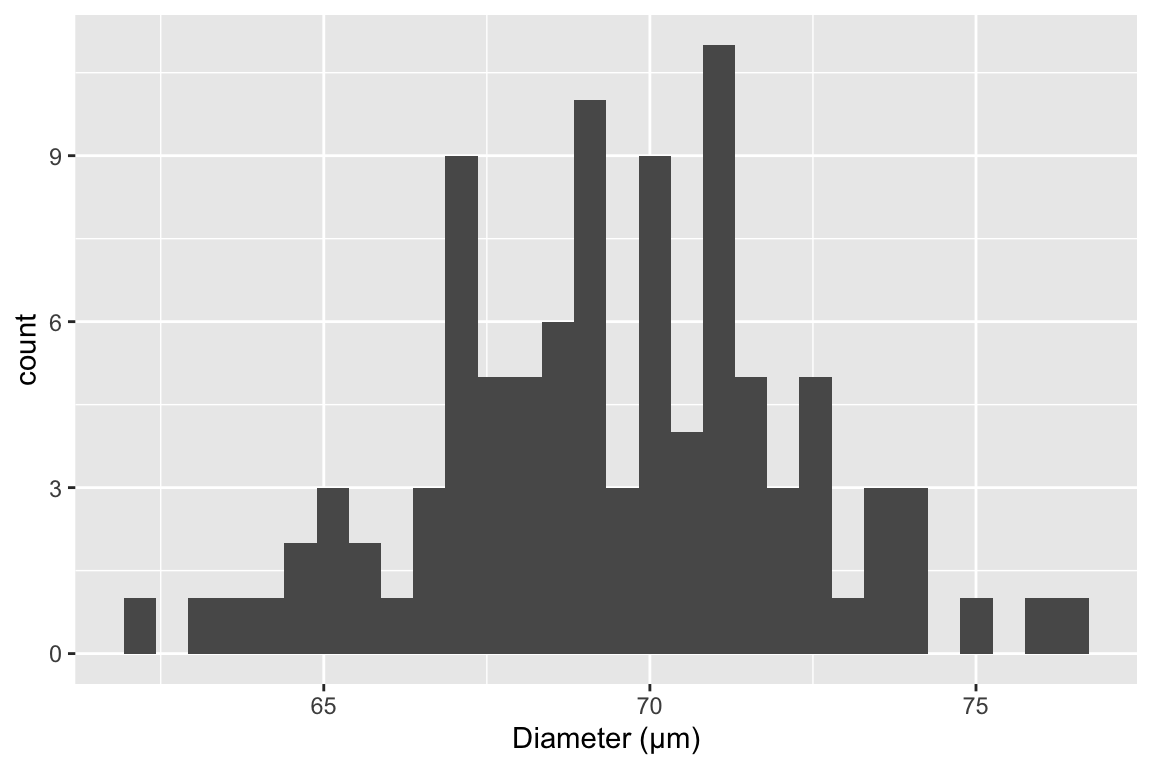
\includegraphics{Walker-elementary-statistical-modeling-draft_files/figure-latex/histogram-1.pdf}

The mean of this sample is 69.4 and the standard deviation is 2.8. The
standard deviation is the square root of the variance, and so computed
by

\begin{equation}
s_y = \sqrt{\frac{\sum_{i=1}^n{(y_i - \overline{y})^2}}{n-1}}
\label{eq:variance}
\end{equation}

Memorize this equation. To understand the logic of this measure of
variability, note that \(y_i - \overline{y}\) is the \textbf{deviation}
of the \(i\)th value from the sample mean, so the numerator is the sum
of squared deviations. The numerator is a sum over \(n\) items and the
denominator is \(n-1\) so the variance is (almost!) an averaged squared
deviation. More variable samples will have bigger deviations and,
therefore, bigger average squared deviations. Since the standard
deviation is the square root of the variance, a standard deviation is
the square root of an average squared deviation. This makes it similar
in value to the averaged deviation (or average of the absolute values of
the deviations since the average deviation is, by definition of a mean,
zero).

Notes on the variance and standard deviation

\begin{enumerate}
\def\labelenumi{\arabic{enumi}.}
\tightlist
\item
  Variances are additive but standard deviations are not. This means
  that the variance of the sum of two independent (uncorrelated) random
  variables is simply the sum of the variances of each of the variables.
  This is important for many statistical analyses.
\item
  The units of variance are the square of the original units, which is
  awkward for interpretation. The units of a standard deviation is the
  same as that of the original variable, and so is much easier to
  interpet.
\item
  For variables that are approximately normally distributed, we can map
  the standard deviation to the quantiles of the distribution. For
  example, 68\% of the values are within one standard deviation of the
  mean, 95\% of the values are within two standard deviations, and 99\%
  of the values are within three standard deviations.
\end{enumerate}

\subsection{Standard error of the
mean}\label{standard-error-of-the-mean}

A standard error of a statistic is a measure of the precision of the
statistic. The standard error of the mean is a measure of the precision
of the estimate of the mean. The smaller the standard error, the more
precise the estimate. The standard error of the mean (SEM) is computed
as

\begin{equation}
SEM = \frac{s_y}{\sqrt{n}}
\label{eq:se}
\end{equation}

The SEM is often denoted \(s_{\bar{y}}\) to indicate that it is a
standard deviation of the mean (\(\bar{y}\)). In what sense is a
standard error a measure of variability? This is kinda weird. If we
sample 100 cells in the slide of muscle tissue and compute the mean
diameter, how can the mean have a standard deviation? There is only one
value! To understand how the SEM is a standard deviation, imagine 1)
resampling 100 cells and 2) recomputing a mean from the re-sampled data,
then repeating this resampling and recomputation an infinite number of
times and each time, you write down the newly computed mean. The true
standard error of the mean is the standard deviation of this infinitely
long column of means. This means that a standard error of the mean,
computed from a single sample using equation \eqref{eq:se} is itself a
sample statistic.

Notes on standard errors

\begin{enumerate}
\def\labelenumi{\arabic{enumi}.}
\tightlist
\item
  The SEM is only one kind of standard error. A standard deviation can
  be computed for any statistic -- these are all standard errors. For
  some statistics, such as the mean, the standard error can be computed
  directly using an equation, such as that for the SEM (equation
  \eqref{eq:se}. For other statistics, a computer intensive method such as
  the \textbf{bootstrap} is necessary to compute a standard error. We
  will return to the bootstrap at the end of this chapter.
\item
  The units of a standard error are the units of the measured variable.
\item
  A standard error is proportional to sample variability (the sample
  standard deviation, \(s_y\)) and inversely proportional to sample size
  (\(n\)). Sample variability is a function of both natural variation
  (there really is variation in diameter among fibers in the quadriceps
  muscle) and measurement error (imaging software with higher resolution
  can measure a diameter with less error). Since the SEM is a measure of
  the precision of estimating a mean, this means this precision will
  increase (or the SEM will decrease) if 1) an investigator uses methods
  that reduce measurement error and 2) an investigator computes the mean
  from a larger sample.
\item
  This last point (the SEM decreases with sample size) seems obvious
  when looking at equation \eqref{eq:se}, since \(n\) is in the
  denominator. Of course \(n\) is also in the denominator of equation
  \eqref{eq:variance} for the sample standard deviation but the standard
  deviation does not decrease as sample size increases. First this
  wouldn't make any sense -- variability is variability. A sample of
  10,000 cell diameters should be no more variable than a sample of 100
  cell diameters (think about if you agree with this or not). Second,
  this should also be obvious from equation \eqref{eq:variance}. The
  standard deviation is the square root of an average and averages don't
  increase with the number of things summed since both the the numerator
  (a sum) and denominator increase with \(n\).
\end{enumerate}

\section{Using Google Sheets to generate fake data to explore
uncertainty}\label{using-google-sheets-to-generate-fake-data-to-explore-uncertainty}

In statistics we are interested in estimated parameters of a
\textbf{population} using measures from a \textbf{sample}. The goal in
this section is to use Google Sheets (or Microsoft Excel) to use fake
data to discover the behavior of sampling and to gain some intuition
about uncertainty using standard errors.

\subsection{Steps}\label{steps}

\begin{enumerate}
\def\labelenumi{\arabic{enumi}.}
\tightlist
\item
  Open Google Sheets
\item
  In cell A1 type ``mu''. mu is the greek letter \(\mu\) and is very
  common notation for the poplation value (the TRUE value!) of the mean
  of some hypothetical measure. In cell B1, insert some number as the
  value of \(\mu\). Any number! It can be negative or positive.
\item
  In cell A2 type ``sigma''. sigma is the greek letter \(\sigma\).
  \(\sigma^2\) is very common (universal!) notation for the population
  (TRUE) variance of some measure or parameter. Notice that the true
  (population) values of the mean and variance are greek letters. This
  is pretty standard in statistics. In cell B2, insert some positive
  number (standard deviations are the positive square roots of the
  variance).
\item
  In cell A8 type the number 1
\item
  In cell A9 insert the equation ``=A8 + 1''. What is this equation
  doing? It is adding the number 1 to to the value in the cell above, so
  the resulting value should be 2.
\item
  In Cell B8, insert the equation ``=normsinv(rand())*\$B\$2 + \$B\$1``.
  The first part of the equation creates a random normal variable with
  mean 0 and standard deviation 1. multiplication and addition transform
  this to a random normal variable with mean \(\mu\) and standard
  deviation \(\sigma\) (the values you set in cells B1 and B2).
\item
  copy cell B8 and paste into cell B9. Now Higlight cells A9:B9 and copy
  the equations down to row 107. You now have 100 random variables
  sampled from a infinite population with mean \(\mu\) and standard
  deviation \(\sigma\).
\item
  In cell A4 write ``mean 10''. In cell B4 insert the equation
  ``=average(B8:B17)''. The resulting value is the \textbf{sample mean}
  of the first 10 random variables you created. Is the mean close to
  \(\mu\)?
\item
  In cell A5 write ``sd 10''. In cell B5 insert the equation
  ``stdev(B8:B17)''. The result is the \textbf{sample standard
  deviation} of the first 10 random variables. Is this close to
  \(\sigma\)?
\item
  In cell A6 write ``mean 100''. In cell B6 insert the equation
  ``=average(B8:B107)''. The resulting value is the \textbf{sample mean}
  of the all 100 random variables you created. Is this mean closer to
  \(\mu\) than mean 10?
\item
  In cell A7 write ``sd 100''. In cell B7 insert the equation
  ``=stdev(B8:B107)''. The resulting value is the \textbf{sample
  standard deviation} of the all 100 random variables you created. Is
  this SD closer to \(\sigma\) than sd 10?
\end{enumerate}

The sample standard deviation is a measure of the variability of the
sample. The more spread out the sample (the further each value is from
the mean), the bigger the sample standard deviation. The sample standard
deviation is most often simply known as ``The'' standard deviation,
which is a bit misleading since there are many kinds of standard
deviations!

Remember that your computed mean and standard deviations are estimates
computed from a sample. They are estimates of the true values \(\mu\)
and \(\sigma\). Explore the behavior of the sample mean and standard
deviation by re-calculating the spreadsheet. In Excel, a spreadsheet is
re-calculated by simultaneously pressing the command and equal key. In
Google, command-R recalculates but is painfully slow. Instead, if using
Google Sheets, just type the number 1 into a blank cell, and the sheet
recalculates quickly. Do it again. And again.

Each time you re-calculate, a new set of random numbers are generated
and the new means and standard deviations are computed. Compare mean 10
and mean 100 each re-calculation. Notice that these estimates are
variable. They change with each re-calculation. How variable is mean 10
compared to mean 100? The variability of the estimate of the mean is a
measure of \textbf{uncertainty} in the estimate. Are we more uncertain
with mean 10 or with mean 100? This variability is measured by a
standard deviation. This \textbf{standard deviation of the mean} is also
called the \textbf{standard error of the mean}. Many researchers are
loose with terms and use ``The'' standard error to mean the standard
error of the mean, even though there are many kinds of standard errors.
In general, ``standard error''" is abbreviated as ``SE.'' Sometimes
``standard error of the mean'' is specifically abbreviated to ``SEM.''

The standard error of the mean is a measure of the precision in
estimating the mean. The smaller the value the more precise the
estimate. The standard error of the mean \emph{is} a standard deviation
of the mean. This is kinda weird. If we sample a population one time and
compute a mean, how can the mean have a standard deviation? There is
only one value! And we compute this value using the sample standard
deviation: \(SEM = \frac{SD}{\sqrt{N}}\). To understand how the SEM is a
standard deviation, Imagine recalculating the spread sheet an infinite
number of times and each time, you write down the newly computed mean.
The standard error of the mean is the standard deviation of this
infinitely long column of means.

\section{Using R to generate fake data to explore
uncertainty}\label{using-r-to-generate-fake-data-to-explore-uncertainty}

note that I use ``standard deviation'' to refer to the sample standard
deviation and ``standard error'' to refer to the standard error of the
mean (again, we can compute standard errors as a standard deviation of
any kind of estimate)

\subsection{part I}\label{part-i}

In the exercise above, you used Google Sheets to generate \(p\) columns
of fake data. Each column had \(n\) elements, so the matrix of fake data
was \(n \times m\) (it is standard in most fields to specify a matrix as
rows by columns). This is \emph{much} easier to do in R and how much
grows exponentially as the size of the matrix grows.

To start, we just generate a \(n \times p\) matrix of normal random
numbers.

\begin{Shaded}
\begin{Highlighting}[]
\CommentTok{# R script to gain some intuition about standard deviation (sd) and standard error (se)}
\CommentTok{# you will probably need to install ggplot2 using library(ggplot2) }
\NormalTok{n <-}\StringTok{ }\DecValTok{6} \CommentTok{# sample size}
\NormalTok{p <-}\StringTok{ }\DecValTok{100} \CommentTok{# number of columns of fake data to generate}
\NormalTok{fake_data <-}\StringTok{ }\KeywordTok{matrix}\NormalTok{(}\KeywordTok{rnorm}\NormalTok{(n}\OperatorTok{*}\NormalTok{p, }\DataTypeTok{mean=}\DecValTok{0}\NormalTok{, }\DataTypeTok{sd=}\DecValTok{1}\NormalTok{), }\DataTypeTok{nrow=}\NormalTok{n, }\DataTypeTok{ncol=}\NormalTok{p) }\CommentTok{# create a matrix}
\end{Highlighting}
\end{Shaded}

the 3rd line is the cool thing about R. In one line I'm creating a
dataset with \(n\) rows and \(p\) columns. Each column is a sample of
the standard normal distribution which by definition has mean zero and
standard deviation of 1. But, and this is important, any sample from
this distribution will not have exactly mean zero and standard deviation
of 1, because it's a sample, the mean and standard deviation will have
some small errror from the truth. The line has two parts to it: first
I'm using the function ``rnorm'' (for random normal) to create a vector
of n*m random, normal deviates (draws from the random normal
distribution) and then I'm organizing these into a matrix (using the
function ``matrix'')

To compute the vector of means, standard deviations, and standard errors
for each column of \texttt{fake\_data}, use the \texttt{apply()}
function.

\begin{Shaded}
\begin{Highlighting}[]
\NormalTok{means <-}\StringTok{ }\KeywordTok{apply}\NormalTok{(fake_data,}\DecValTok{2}\NormalTok{,mean) }\CommentTok{# the apply function is super useful}
\NormalTok{sds <-}\StringTok{ }\KeywordTok{apply}\NormalTok{(fake_data,}\DecValTok{2}\NormalTok{,sd)}
\NormalTok{sems <-}\StringTok{ }\NormalTok{sds}\OperatorTok{/}\KeywordTok{sqrt}\NormalTok{(n)}
\end{Highlighting}
\end{Shaded}

\texttt{apply()} is a workhorse in many R scripts. Learn it. Know it.
Live it.

The SEM is the standard deviation of the mean, so let's see if the
standard deviation of the means is close to the true standard error. We
sampled from a normal distribution with SD=1 so the true standard is

\begin{Shaded}
\begin{Highlighting}[]
\DecValTok{1}\OperatorTok{/}\KeywordTok{sqrt}\NormalTok{(n)}
\end{Highlighting}
\end{Shaded}

\begin{verbatim}
## [1] 0.4082483
\end{verbatim}

and the standard deviation of the \(p\) means is

\begin{Shaded}
\begin{Highlighting}[]
\KeywordTok{sd}\NormalTok{(means)}
\end{Highlighting}
\end{Shaded}

\begin{verbatim}
## [1] 0.3731974
\end{verbatim}

Questions

\begin{enumerate}
\def\labelenumi{\arabic{enumi}.}
\tightlist
\item
  how close is \texttt{sd(means)} to the true SE?
\item
  change p above to 1000. Now how close is sd(means) to the true SE?
\item
  change p above to 10,000. Now how close is sd(means) to the true SE?
\end{enumerate}

\subsection{part II - means}\label{part-ii---means}

This is a visualization of the spread, or variability, of the sampled
means

\begin{Shaded}
\begin{Highlighting}[]
\KeywordTok{qplot}\NormalTok{(means)}
\end{Highlighting}
\end{Shaded}

\begin{verbatim}
## `stat_bin()` using `bins = 30`. Pick better value with `binwidth`.
\end{verbatim}

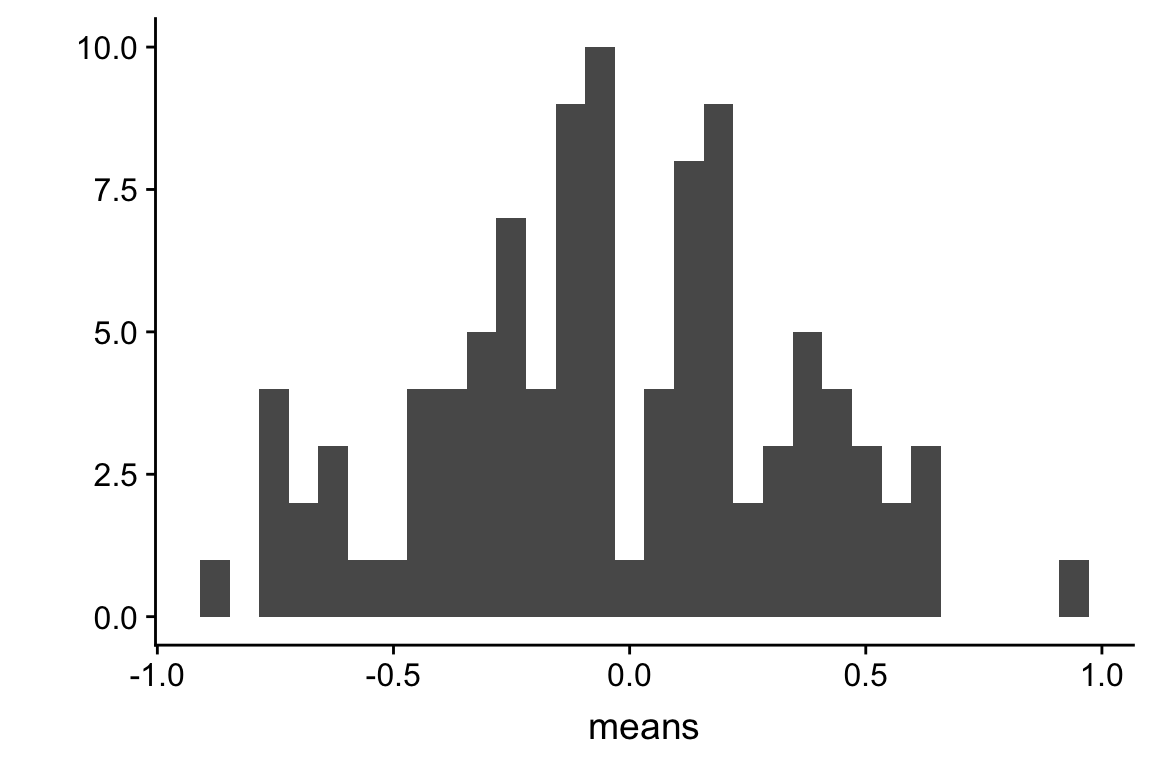
\includegraphics{Walker-elementary-statistical-modeling-draft_files/figure-latex/unnamed-chunk-6-1.pdf}

Compute the mean of the means

\begin{Shaded}
\begin{Highlighting}[]
\KeywordTok{mean}\NormalTok{(means)}
\end{Highlighting}
\end{Shaded}

\begin{verbatim}
## [1] -0.039961
\end{verbatim}

Questions

\begin{enumerate}
\def\labelenumi{\arabic{enumi}.}
\tightlist
\item
  Remember that the true mean is zero. How close, in general, are the
  sampled means to the true mean. How variable are the means? How is
  this quantified?
\item
  change n to 100, then replot. Are the means, in general, closer to the
  true mean? How variable are the means now?
\item
  Is the mean estimated with \(n=100\) closer to the truth, in general,
  then the mean estimated with \(n=6\)?
\item
  Redo with \(n=10000\)
\end{enumerate}

\subsection{part III - how do SD and SE change as sample size (n)
increases?}\label{part-iii---how-do-sd-and-se-change-as-sample-size-n-increases}

\begin{Shaded}
\begin{Highlighting}[]
\KeywordTok{mean}\NormalTok{(sds)}
\end{Highlighting}
\end{Shaded}

\begin{verbatim}
## [1] 1.017144
\end{verbatim}

Questions

\begin{enumerate}
\def\labelenumi{\arabic{enumi}.}
\tightlist
\item
  what is the mean of the standard deviations when n=6 (set p=1000)
\item
  what is the mean of the standard deviations when n=100 (set p=1000)
\item
  when n = 1000? (set p=1000)
\item
  when n = 10000? (set p=1000)
\item
  how does the mean of the standard deviations change as n increases
  (does it get smaller? or stay about the same size)
\item
  repeat the above with SEM
\end{enumerate}

\begin{Shaded}
\begin{Highlighting}[]
\KeywordTok{mean}\NormalTok{(sems)}
\end{Highlighting}
\end{Shaded}

\begin{verbatim}
## [1] 0.4152472
\end{verbatim}

Congratulations, you have just done a Monte Carlo simulation!

\subsection{\texorpdfstring{Part IV -- Generating fake data with ``for
loops''}{Part IV -- Generating fake data with for loops}}\label{part-iv-generating-fake-data-with-for-loops}

\begin{Shaded}
\begin{Highlighting}[]
\NormalTok{n <-}\StringTok{ }\DecValTok{6} \CommentTok{# sample size}
\NormalTok{n_iter <-}\StringTok{ }\DecValTok{10}\OperatorTok{^}\DecValTok{5} \CommentTok{# number of iterations of loop (equivalent to p)}
\NormalTok{means <-}\StringTok{ }\KeywordTok{numeric}\NormalTok{(n_iter)}
\NormalTok{sds <-}\StringTok{ }\KeywordTok{numeric}\NormalTok{(n_iter)}
\NormalTok{sems <-}\StringTok{ }\KeywordTok{numeric}\NormalTok{(n_iter)}
\ControlFlowTok{for}\NormalTok{(i }\ControlFlowTok{in} \DecValTok{1}\OperatorTok{:}\NormalTok{n_iter)\{}
\NormalTok{  y <-}\StringTok{ }\KeywordTok{rnorm}\NormalTok{(n) }\CommentTok{# mean=0 and sd=1 are default so not necessary to specify}
\NormalTok{  means[i] <-}\StringTok{ }\KeywordTok{mean}\NormalTok{(y)}
\NormalTok{  sds[i] <-}\StringTok{ }\KeywordTok{sd}\NormalTok{(y)}
\NormalTok{  sems[i] <-}\StringTok{ }\KeywordTok{sd}\NormalTok{(y)}\OperatorTok{/}\KeywordTok{sqrt}\NormalTok{(n)}
\NormalTok{\}}
\KeywordTok{sd}\NormalTok{(means)}
\end{Highlighting}
\end{Shaded}

\begin{verbatim}
## [1] 0.4090702
\end{verbatim}

\begin{Shaded}
\begin{Highlighting}[]
\KeywordTok{mean}\NormalTok{(sems)}
\end{Highlighting}
\end{Shaded}

\begin{verbatim}
## [1] 0.3883867
\end{verbatim}

Questions

\begin{enumerate}
\def\labelenumi{\arabic{enumi}.}
\tightlist
\item
  What do \texttt{sd(means)} and \texttt{mean(sems)} converge to as
  \texttt{n\_iter} is increased from 100 to 1000 to 10,000?
\item
  Do they converge to the same number?
\item
  Should they?
\item
  What is the correct number?
\end{enumerate}

Question number 4 is asking what is E(SEM), the ``expected standard
error of the mean''. There is a very easy formula to compute this. What
is it?

\section{Bootstrapped standard
errors}\label{bootstrapped-standard-errors}

The bootstrap is the best invention since duct tape. Really.

A standard error is the standard deviation of an infinite number of
hypothetically re-sampled means. A bootstrap standard error of a
statistic is the standard deviation of the statistic from a finite
number of resamples of the data! Wait what?

Let's download some data to explore this concept. The data are archived
at Dryad Repository.

\begin{enumerate}
\def\labelenumi{\arabic{enumi}.}
\tightlist
\item
  URL: \url{https://datadryad.org//resource/doi:10.5061/dryad.31cc4}
\item
  file: RSBL-2013-0432 vole data.xlsx
\item
  sheet: COLD VOLES LIFESPAN
\end{enumerate}

The data are the measured lifespans of the short-tailed field vole
(\emph{Microtus agrestis}) under three different experimental
treatments: vitamin E supplementation, vitamin C supplementation, and
control (no vitamin supplementation). Vitamins C and E are antioxidants,
which are thought to be protective of basic cell function since they
bind to the cell-damaging reactive oxygen species that result from cell
metabolism.

I've read in the file using read\_excel and converted to a data.table
named \texttt{vole}. I used \texttt{setnames} to rename the columns to
lifespan, control, vitamin\_E, and vitamin\_C. The data are in a
\textbf{wide format} -- that is instead of a single ``treatment''
column, there are three columns (``control'', ``vitamin C'', ``vitamin
E'') with value = 1, if that row (or lifespan) was assigned the
treatment of the column label and zero otherwise. In general, we want
data.tables to be in long format. Wide formats can be useful for some
computations but not really for these data.

Compute the standard error of the mean of the lifespan for the control
group using equation \eqref{eq:se}. One simple way to do this for the
control group is to extract the subset of the data satisfying the
condition control = 1 (the value in the column ``control'' equals 1). In
R, these conditional querries use \texttt{==}.

\begin{Shaded}
\begin{Highlighting}[]
\NormalTok{y <-}\StringTok{ }\KeywordTok{na.omit}\NormalTok{(vole[control}\OperatorTok{==}\DecValTok{1}\NormalTok{, lifespan]) }\CommentTok{# subset of data satisfying condition and omitting missing data, if these exist}
\NormalTok{n <-}\StringTok{ }\KeywordTok{length}\NormalTok{(y) }\CommentTok{# the sample size}
\NormalTok{se <-}\StringTok{ }\KeywordTok{sd}\NormalTok{(y)}\OperatorTok{/}\KeywordTok{sqrt}\NormalTok{(n}\OperatorTok{-}\DecValTok{1}\NormalTok{) }\CommentTok{# standard error of the mean}
\end{Highlighting}
\end{Shaded}

Okay, the SEM using equation \eqref{eq:se} is 31.9. Let's compare this
with a bootstrap estimate of the SEM.

\begin{Shaded}
\begin{Highlighting}[]
\NormalTok{n_iter <-}\StringTok{ }\DecValTok{2000} \CommentTok{# number of bootstrap iterations}
\NormalTok{means <-}\StringTok{ }\KeywordTok{numeric}\NormalTok{(n_iter) }\CommentTok{# we will save the means each iteration to this}
\NormalTok{inc <-}\StringTok{ }\DecValTok{1}\OperatorTok{:}\NormalTok{n }\CommentTok{# the first sample is the actual sample}
\ControlFlowTok{for}\NormalTok{(iter }\ControlFlowTok{in} \DecValTok{1}\OperatorTok{:}\NormalTok{n_iter)\{ }\CommentTok{# the for loop}
\NormalTok{  means[iter] <-}\StringTok{ }\KeywordTok{mean}\NormalTok{(y[inc])}
\NormalTok{  inc <-}\StringTok{ }\KeywordTok{sample}\NormalTok{(}\DecValTok{1}\OperatorTok{:}\NormalTok{n, }\DataTypeTok{replace=}\OtherTok{TRUE}\NormalTok{) }\CommentTok{# re-sample for the next iteration}
\NormalTok{\}}
\NormalTok{se_boot <-}\StringTok{ }\KeywordTok{sd}\NormalTok{(means)}

\CommentTok{#compare}
\NormalTok{se}
\end{Highlighting}
\end{Shaded}

\begin{verbatim}
## [1] 31.89536
\end{verbatim}

\begin{Shaded}
\begin{Highlighting}[]
\NormalTok{se_boot}
\end{Highlighting}
\end{Shaded}

\begin{verbatim}
## [1] 30.93843
\end{verbatim}

dayum!

\chapter{Covariance and Correlation}\label{covariance-and-correlation}

Variance is one of two major concepts in statistical modeling. The
second is \textbf{covariance}, which arises when two variables measured
on the same unit vary together. ``Vary together'' means that if we
measured leg length and arm length on each individual in a sample of
humans, we'd expect individuals with long arms to also have long legs
while those with short arms to have short legs. ``Measured on the same
unit'' means that we measure both leg length and arm length in each
individual of a sample -- we cannot compute a covariance if we measure
legs in one sample and arms in a second. Covariance can be positive or
negative. It is positive when the tendency is for both values to be
large or both values to be small. It is negative when the tendency is
for one value to be small when the other is large. Positive and negative
covariance are easily visualized with a scatterplot
\ref{fig:covariance-scatterplot}.

\begin{figure}
\centering
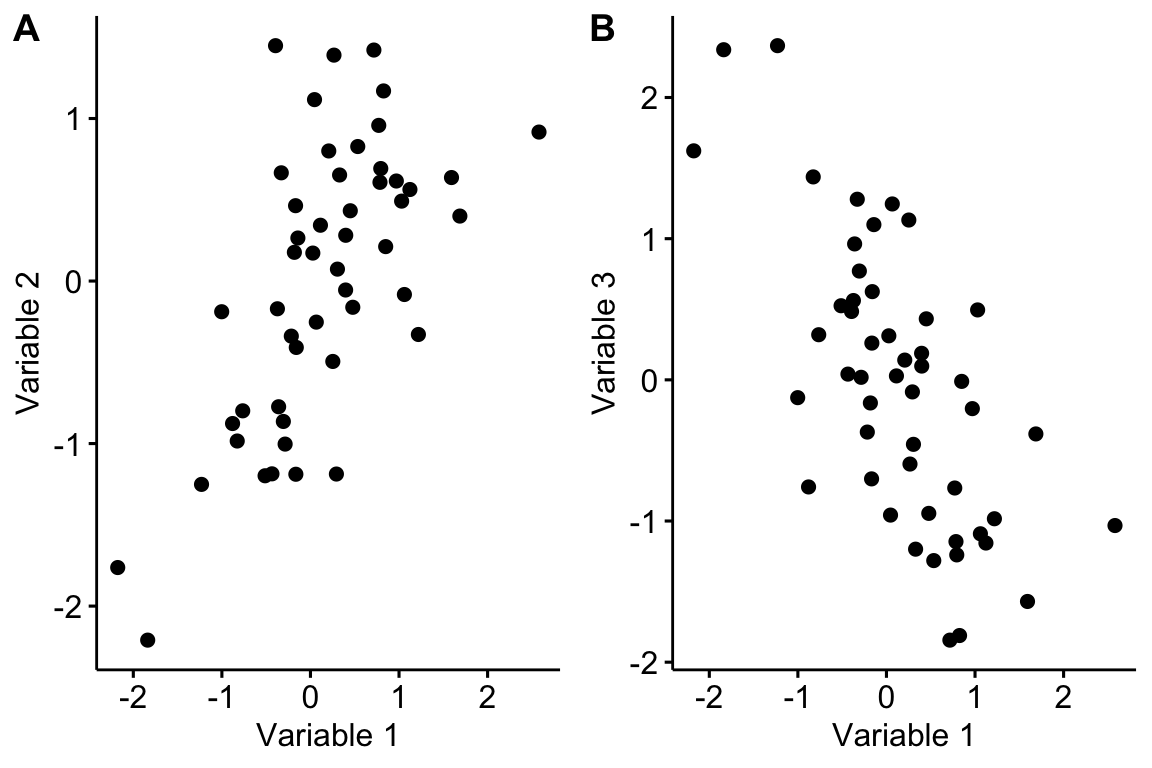
\includegraphics{Walker-elementary-statistical-modeling-draft_files/figure-latex/covariance-scatterplot-1.pdf}
\caption{\label{fig:covariance-scatterplot}Scatterplot illustrating two
variables with (A) positive covariance and (B) negative covariance}
\end{figure}

\section{}\label{section}

\begin{enumerate}
\def\labelenumi{\arabic{enumi}.}
\tightlist
\item
  Covariance
\end{enumerate}

\begin{equation}
\mathrm{COV}[X, Y] = \sum_{i=1}^n{\frac{(x_i - \bar{x})(y_i - \bar{y})}{n-1}}
\label{eq:cov}
\end{equation}

Compare this to the equation for the variance. In \eqref{eq:cov}, the
numerator in the sum is the product of two different deviations (one for
each variable) instead of the product of a deviation with itself.

\begin{enumerate}
\def\labelenumi{\arabic{enumi}.}
\setcounter{enumi}{1}
\item
  Correlation
\item
  Regression
\end{enumerate}

\chapter{P-values}\label{p-values}

\section{\texorpdfstring{\(p\)-values}{p-values}}\label{p-values}

\begin{tabular}{l|r|r|r|r|r|r|r}
\hline
contrast & estimate & SE & df & lower.CL & upper.CL & t.ratio & p.value\\
\hline
vitamin\_E - control & -89.9 & 52 & 93 & -194.1 & 14.3 & -1.7 & 0.090\\
\hline
vitamin\_C - control & -115.1 & 54 & 93 & -223.2 & -6.9 & -2.1 & 0.037\\
\hline
vitamin\_C - vitamin\_E & -25.2 & 65 & 93 & -154.1 & 103.8 & -0.4 & 0.699\\
\hline
\end{tabular}

Let's use the vole data to introduce the \(p\)-value. The table above
gives a SE, \(t\) and \(p\)-value for each pairwise contrast among the
three treatment levels. A typical report (one with several
misconceptions) might read

``We found a significant effect of Vitamin C (\(t=\) -2.1, \(p=\) 0.037)
on lifespan, but no effect of vitamin E (\(t=\) -1.7, \(p=\) 0.09) on
lifespan.''

A \(p\) value \emph{is a continuous measure of evidence against the
null}. As long as the data approximate the assumptions of the null
hypothesis pretty well, a very small \(p\)-value, such as 0.002 or
0.0005, is pretty good evidence against the null hypothesis -- but does
not mean ``an effect exists''. To show an effect exists, we should have
small \(p\)-values in multiple replicates \emph{and} we should
rigorously probe the hypothesis with different experiments that
challenge the hypothesis in different ways. A small \(p\) is evidence
for a research program to move forward with replication and probing. A
big \(p\)-value, say 0.22 or 0.76, is pretty weak evidence against the
null, but does not mean ``there is no effect.'' If an experiment is well
designed, a big \(p\) could suggest abandoning any hypotheses that
predict biologically consequential effects. Unfortunately, a big \(p\)
could also reflect a weak experimental design. Between small and big
\(p\) values, such as 0.009 or 0.011, problems arise. These intermediate
\(p\)-values beg for replication. A major problem of inference using
\(p\) values is that there is no sharp boundaries between these three
regions. Instead biologists typically use the \(p < 0.05\) as a sharp
boundary to declare that an effect exists or not.

Okay. so what \emph{is} a \(p\)-value? When we do a \(t\)-test, we get a
\(p\)-value. There are several ways to think about this probability. The
most compact way is \(P(data | null)\), which is literally read as the
probability of the data given the null (or ``conditional'' on the null),
but is really short for \emph{the probability of the data, or something
more extreme than the data, given that the null hypothesis is true}. The
``probability of the data'' is kinda vague. More specifically, we mean
the probability of some statistic about the data such as the difference
in means between group A and group B or the \(t\)-value associated with
this difference. So, a bit more formally, the probability returned in a
\(t\)-test is \(\mathrm{prob}(t \ge t_{obs} | H_0)\). This is the long
run frequency of observing a \(t\)-value as big or bigger than the
observed \(t\)-value (the one you actually got with your data) if the
null is true. Let's parse this into ``long run frequency of observing a
\(t\)-value as big or bigger than the observed \(t\)-value'' and ``null
is true''.

A thought experiment: You open a google sheet and insert 12 standard,
normal random deviates (so the true mean is zero and the true variance
is one) in Column A, rows 1-12. You arbitrarily assign the first six
values (rows 1-6) to treatment A and the second six values (rows 7-12)
to treatment B. You use the space immediately below these data to
compute the mean of treatment A, the mean of treatment B, the difference
in means (A - B), and a \(t\)-value. Unfortunately, google sheets
doesn't have a \(t\)-value function so you'd have to compute this
yourself. Or not, since this is a thought experiment. Now ``fill right''
or copy and paste these functions into 999 new columns. You now have
1000 \(t\) tests. The expected value of the difference in means is zero
(why?) but the actual values will form a normal distribution about zero.
Most will be close to zero (either in the negative or positive
direction) but some will be further from zero. The expected \(t\)-value
will also be zero (why?) and the distribution of these 1000 \(t\) values
will look normal but the tails are a little fuller. This row of \(t\)
values is a null distribution, because in generating the data we used
the exact same formula for the values assigned to A and the values
assigned to B. Now think of a \(t\)-value in your head, say 0.72
(remember that \(t\) values will largely range from about -3 to +3
although the theoretical range is \(-\infty\) to \(+\infty\). What is
the probability of observing a \(t\) of 0.72 \emph{or bigger} if the
null is true? Look at the row of \(t\)-values! Count the number of
\(t \ge 0.72\) and then divide by the total number of \(t\)-values in
the row (1000) and you have a probability computed as a frequency. But
remember the frequentist definition is the long run frequency, or the
expected frequency at the limit (when you've generated not 1000 or even
1,000,000 but an infinite number of columns and \(t\)-values).

Some asides to the thought experiment: First, why ``as big or bigger''
and not just the probability of the value itself? The reason is that the
probability of finding the exact \(t\) is 1/infinity, which doesn't do
us much good. So instead we compute the probability of finding \(t\) as
big, or bigger, than our observed \(t\). Second, the \(t\)-test
probability described above is a ``one-tail probability''. Because a
difference can be both in the positive direction and the negative
direction, we usually want to count all the \(t \ge 0.72\) and the
\(t \le -0.72\) and then add these two counts to compute the frequency
of \emph{as extreme or more extreme} values. This is called a
``two-tailed probability'' because we find extremes at both tails of the
distribution. Third, we don't really count \(t \ge 0.72\) but take
advantage of the beautiful mathematical properties of the theoretical
\(t\) distribution, which allows us to compute the frequentist
probability (expected long range frequency) given the \(t\)-value and
the degrees of freedom using the \(t\)-distribution.

Now what do I mean with the phrase ``null is true''? Most people equate
``null is true'' with ``no difference in means'' but the phrase entails
much more than this. Effectively, the phrase means that the \(p\)-value
is based on modeling the real data with a theoretical sample in which
all the points were randomly sampled from the same distribution and that
the assignment of the individual points to treatment was random. This
model means the theoretical sample has three properties: First, random
assignment to treatment after sampling from the same distribution means
that the expected means are the same, or put differently, the expected
difference in means between the assigned groups is zero. Second, random
assignment to treatment after sampling from the same distribution
\emph{also} means that the expected variances of the two groups are
equal. And third, random sampling means that the values of each point
are independent -- we cannot predict the value of one point knowing
information about any other point. \textbf{Here is what is super
important about this}: if we get a really low \(p\)-value, any one of
these consequences may be untrue about our data, for example it could be
that the true means of the two treatment groups really are different, or
it could mean it is the variances that differ between the two groups, or
it could mean that the data (or technically, the errors) are not
independent of each other. This is why we need certain assumptions to
make a \(p\)-value meaningful for empirical data. By assuming
independent error and homogenous (equal) variances in our two samples, a
low \(p\) value is evidence of unequal means.

\section{Creating a null
distribution.}\label{creating-a-null-distribution.}

Let's repeat: A pretty good definition of a \(p\)-value is: the long-run
frequency of observing a test-statistic as large or larger than the
observed statistic, if the null were true. A more succinct way to state
this is

\begin{equation}
p = \mathrm{prob}(t \ge t_o | H_o)
\end{equation}

where \(t\) is a hypothetically sampled \(t\)-value from a null
distribution, \(t_o\) is the observed \(t\)-value, and \(H_o\) is the
null hypothesis. Part of the null hypothesis is the expected value of
the parameter estimated is usually (but not always) zero -- this can be
called the nil null. For example, if there is no vitamin E effect on
lifespan, then the expected difference between the means of the control
and vitamin E treatment levels is zero. Or,

\begin{equation}
\mathrm{E}(\bar{vitamin_E} - \bar{control} | H_o) = 0.0
\end{equation}

let's plot the data and look at the group means. Below is a strip chart
of the vole data with superimposed treatment level means, using the
function \texttt{ggstripchart} from the ggpubr package (can you make
this?). I'm going to refer to this kind of chart as a ``dot plot'',
which is what most biology researchers call this type of chart.

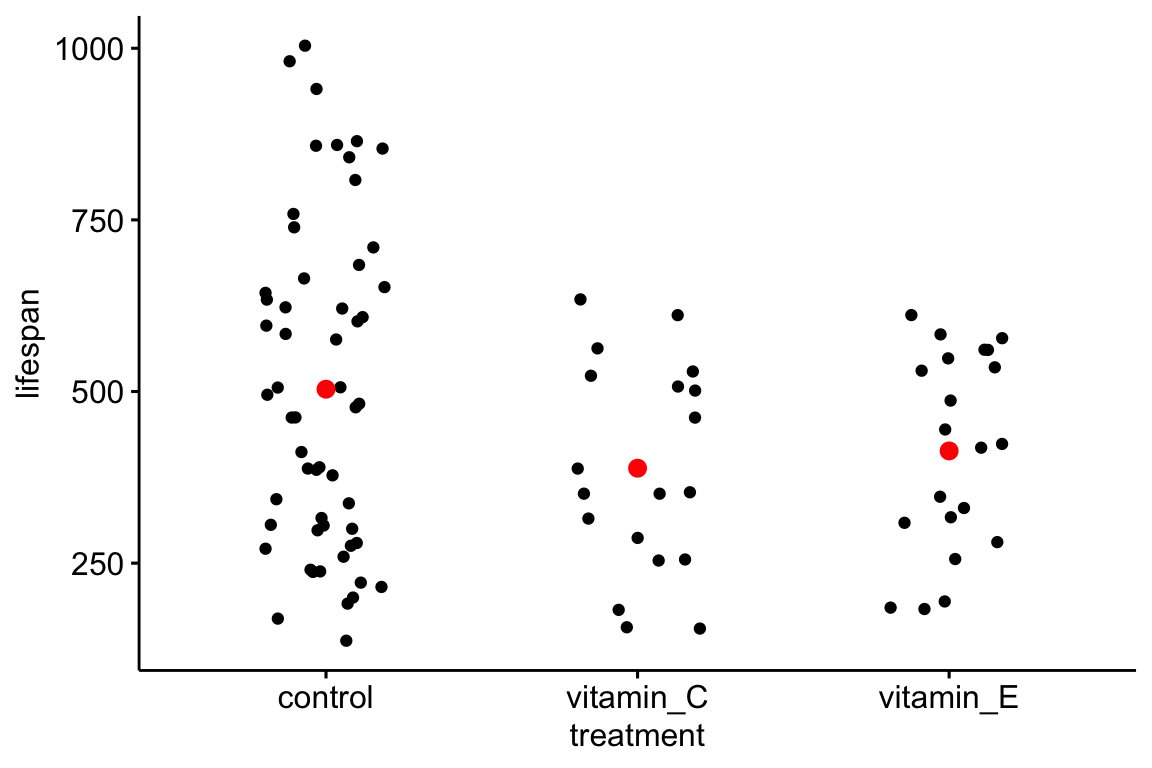
\includegraphics{Walker-elementary-statistical-modeling-draft_files/figure-latex/inference-strip-chart-1.pdf}

\subsection{the Null Distribution}\label{the-null-distribution}

The mean lifespan in the vitamin\_E treatment is -89.9 days shorter than
the mean lifespan in the control treatment. And, the mean lifespan in
the vitamin\_E treatment is -115.1 days shorter than the mean lifespan
in the control treatment. These are the measured effects, or the
\textbf{observed differences in means}. How confident are we in these
effects? Certainly, if the researchers did the experiment with
\emph{two} control treatment groups, they would measure some difference
in their means simply because of finite sampling (more specifically, the
many, many random effects that contribute to lifespan will differ
between the two control groups). So let's reframe the question: are the
observed differences unusually large compared to a distribution of
differences that would occur if there were no effect? That is, if the
``null were true''. To answer this, we compare our observed difference
to this \textbf{null distribution}. This comparison gives the
probability (a long-run frequency) of ``sampling'' a random difference
from the null distribution of differences that is as large, or larger,
than the observed difference.

What is a null distribution? It is the distribution of a statistic (such
as a difference in means, or better, a \(t\)-value) if the null were
true. Here, I am generating a null distribution that is relevant to the
cold vole data. See if you can understand the script before reading the
explanation below.

\begin{Shaded}
\begin{Highlighting}[]
\NormalTok{seed <-}\StringTok{ }\DecValTok{1}
\NormalTok{n_iter <-}\StringTok{ }\DecValTok{10}\OperatorTok{^}\DecValTok{5} \CommentTok{# number of iterations}
\NormalTok{mu <-}\StringTok{ }\KeywordTok{mean}\NormalTok{(vole[treatment}\OperatorTok{==}\StringTok{'control'}\NormalTok{, lifespan]) }
\NormalTok{sigma <-}\StringTok{ }\KeywordTok{sd}\NormalTok{(vole[treatment}\OperatorTok{==}\StringTok{'control'}\NormalTok{, lifespan])}
\NormalTok{n <-}\StringTok{ }\KeywordTok{nrow}\NormalTok{((vole[treatment}\OperatorTok{==}\StringTok{'control'}\NormalTok{,]))}
\NormalTok{sample1 <-}\StringTok{ }\KeywordTok{matrix}\NormalTok{(}\KeywordTok{rnorm}\NormalTok{(n}\OperatorTok{*}\NormalTok{n_iter, }\DataTypeTok{mean=}\NormalTok{mu, }\DataTypeTok{sd=}\NormalTok{sigma), }\DataTypeTok{nrow=}\NormalTok{n) }\CommentTok{# 100,000 samples (each size n)}
\NormalTok{sample2 <-}\StringTok{ }\KeywordTok{matrix}\NormalTok{(}\KeywordTok{rnorm}\NormalTok{(n}\OperatorTok{*}\NormalTok{n_iter, }\DataTypeTok{mean=}\NormalTok{mu, }\DataTypeTok{sd=}\NormalTok{sigma), }\DataTypeTok{nrow=}\NormalTok{n) }\CommentTok{# 100,000 samples}
\NormalTok{null_dis <-}\StringTok{ }\KeywordTok{apply}\NormalTok{(sample2, }\DecValTok{2}\NormalTok{, mean) }\OperatorTok{-}\StringTok{ }\KeywordTok{apply}\NormalTok{(sample1, }\DecValTok{2}\NormalTok{, mean)}
\KeywordTok{qplot}\NormalTok{(null_dis)}
\end{Highlighting}
\end{Shaded}

\begin{figure}
\centering
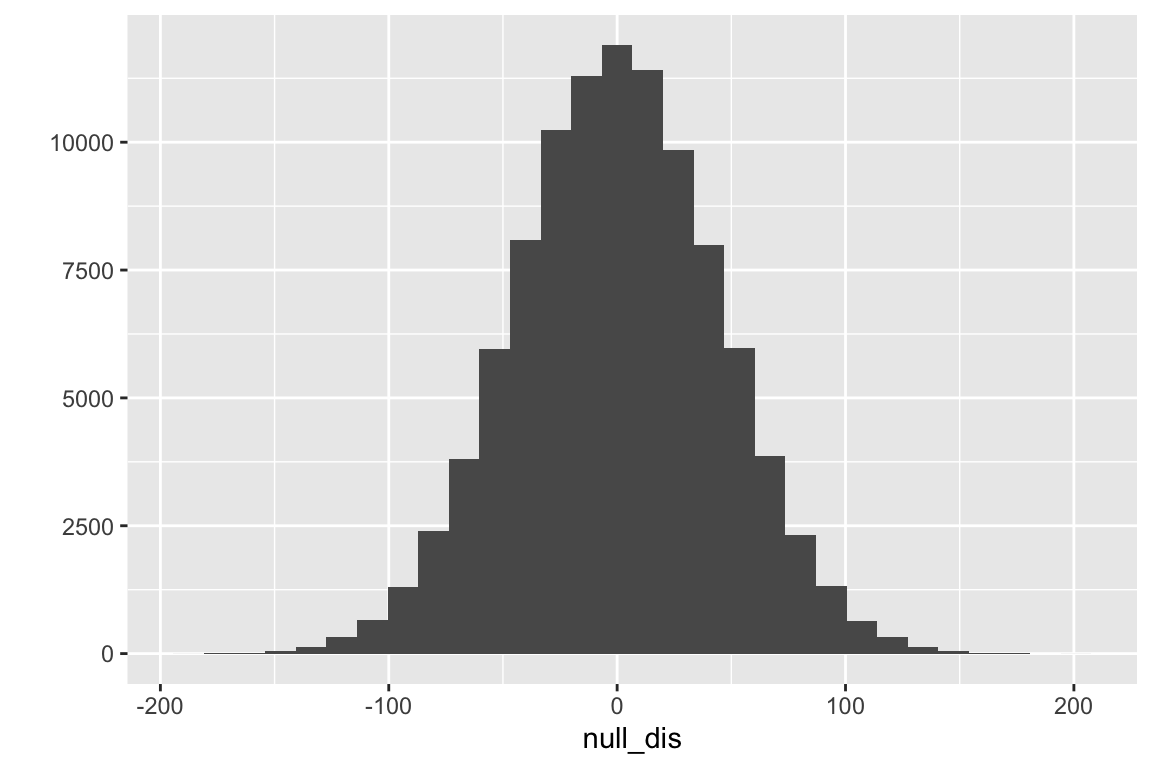
\includegraphics{Walker-elementary-statistical-modeling-draft_files/figure-latex/null-distribution-1.pdf}
\caption{\label{fig:null-distribution}Null distribution for an infinitely
large data set that looks curiously like the lifespans of the cold-rear
voles from the control treatment.}
\end{figure}

What have we done above? We've simulated an infinitely large population
of voles that have a distribution of lifespans similar to that of the
cold-reared voles assigned to the control group. The mean \(\mu\) and
standard deviation \(\sigma\) of the simulated lifespan are equal to the
observed mean and standard deviation of the lifespans of the control
voles. Then, the script:

\begin{enumerate}
\def\labelenumi{\arabic{enumi}.}
\tightlist
\item
  randomly sample 56 values from this population of simulated lifespans
  and assign to sample1. We sample 56 values because that is the sample
  size of our control in the experiment.
\item
  randomly sample 56 values from this population of simulated lifespans
  and assign to sample2.
\item
  compute the difference \(\bar{Y}_{sample2} - \bar{Y}_{sample1}\).
\item
  repeat 1-3 100,000 times, each time saving the difference in means.
\item
  plot the distribution of the 100,000 differences using a histogram
\end{enumerate}

The distribution of the differences is a null distribution. Notice that
the mode of the null distribution is at zero, and the mean (-0.11584) is
close to zero (if we had set \(n\) to infinity, the mean would be
precisely zero). \emph{The expected difference between the means of two
random samples from the same population is, of course, zero}. Don't
gloss over this statement if that is not obvious. The tails extend out
to a little more than +100 and -100. What this means is that it would be
rare to randomly sample two sets of data from the same population with
mean \(\mu\) and standard deviation \(\sigma\) and find a difference of,
say, -257. In fact, in the 100,000 runs, there were no difference as
large as \textbar{}-257\textbar{} (the absolute value of -257). The
minimum and maximum differences sampled over the 100,000 iterations was
-187 days and 201 days.

How do our observed differences compare? Let's focus on vitamin E. The
vitamin\_E effect is -89.9 days. There are 2110 sampled differences less
than the observed value and 2126 greater than the absolute value of the
observed value. Together this is 4236 so the frequency of differences
from the simulated null distribution that as larger or larger than the
observed difference is 0.042 (this compuation includes the observed
value in both the numerator and denominator).

\subsection{\texorpdfstring{\(t\)-tests}{t-tests}}\label{t-tests}

A \(t\)-test is a test of differences between two values. These could be

\begin{enumerate}
\def\labelenumi{\arabic{enumi}.}
\tightlist
\item
  the difference between the means of two samples (a ``two-sample''
  \(t\)-test)
\item
  the difference between a mean of a sample and some pre-specified value
  (a ``one-sample'' \(t\)-test)
\item
  the difference between a coefficient from a linear model and a value
  (often zero)
\end{enumerate}

A \(t\)-test compares an observed \(t\)-value to a \(t\)-distribution.
The null distribution introduced above was a distribution of mean
differences. This isn't generally useful, since the distribution of
expected mean differences is a function of sample variability (standard
deviations) in addition to sample size and, therefore, a mean-difference
null distribution will be unique to every study. A \(t\)-distribution is
a distribution of \(t\)-values under the null (statistical jargon for
``given the null is true''), where a \(t\)-value is a difference
standardized by its standard error. Standardizing by a standard
deviation (remember that a standard error is an estimate of the
statistic's standard deviation) removes the effect of sample variability
on the distribution. A \(t\)-distribution, then, is only a function of
sample size (or ``degrees of freedom''). As \(n\) increases a \(t\)
distribution becomes converges on the standard, normal distribution.

The difference between the mean of the vitamin\_E treatment and the
control treatment is -89.9. A two-sample \(t\)-test of this difference
is

\begin{verbatim}
## 
##  Two Sample t-test
## 
## data:  vole[treatment == "vitamin_E", lifespan] and vole[treatment == "control", lifespan]
## t = -1.6275, df = 75, p-value = 0.1078
## alternative hypothesis: true difference in means is not equal to 0
## 95 percent confidence interval:
##  -199.97362   20.14029
## sample estimates:
## mean of x mean of y 
##  413.4762  503.3929
\end{verbatim}

The \(p\)-value comes from comparing the observed \(t\) to a null \(t\)
distribution and ``counting'' the values that are bigger than the
observed \(t\). These are counted in both tails, because \(p\) is the
probability of a \(t\) more extreme than the observed value, and \(t\)
can be more extreme in the negative direction and in the positive
direction. We can simulate this with a finite, instead of infinite, null
distribution using the t-distribution instead of the distribution of
mean differences, as above. I hide the script, but its the same as
above, except that the \(t\)-value is computed for each simulated
experiment and not just the difference in means.

\begin{figure}
\centering
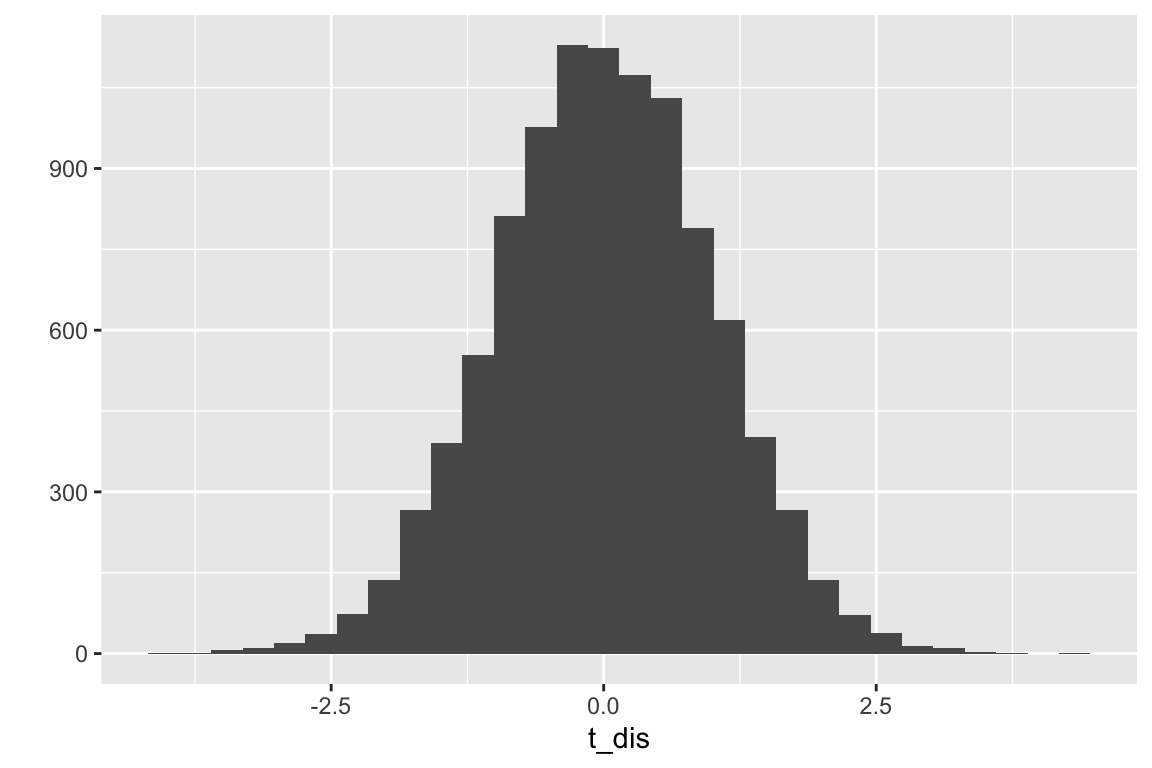
\includegraphics{Walker-elementary-statistical-modeling-draft_files/figure-latex/null-distribution-t-1.pdf}
\caption{\label{fig:null-distribution-t}Null distribution of t-values. The
simulation generated 100,000 t-tests with a true null.}
\end{figure}

Hey that looks pretty good! A \(p\) value can be computed by counting
the number of simulated \(t\)-values, \emph{including the observed
value}, that are more extreme (in either the positive or negative
direction) than the observed \(t\). Including the observed \(t\), there
are 10904 values that are more extreme than that observed. An
approximate measure of \(p\) is this count divided by 100,001 (why is 1
added to the denominator?), which is 0.1090389. This simulation-based
\(p\)-value is very (very!) close to that computed from the observed
\(t\)-test.

\subsection{P-values from the perspective of
permutation}\label{p-values-from-the-perspective-of-permutation}

A very intuitive way to think about \(p\)-values is with a permutation
test. Consider two of the treatment levels in the vole data, say vitamin
E and the vitamin C (I'm bored with the control!). Think about the
structure of the dataset: there are two columns, ``Treatment'', which
contains the assigned treatment, and ``Lifespan''. The values in the
Treatment column were randomly assigned prior to the start of the
experiment. If there is an effect of treatment on lifespan, then
assginment matters -- the values in the lifespan column for the vitamin
E rows will be more or less, on average, than the values in the lifepan
column for the vitamin C rows. Or, the lifespan values are what they are
\emph{because} of the values in the treatment column.

Now let's leave the values in the treatment column be, and just randomly
re-arrange or permute the lifespan values. What is the new expected
diference in lifespan between the two treatments? Zero, of course! That
is, because the lifespans were randomly re-arranged, they cannot be
caused by treatment assignment!

A permutation is a random re-arrangement of values in a column. Consider
the many thousands of permutations of the values in the lifespan column.
A difference in means can be computed from each of these permuations and
a distribution of differences can be generated. Is the observed
difference extreme relative to the other values in this distribution?
This is a permutation test -- it compares an observed statistic to a
distributin of the statistic computed over many thousands of
permutations.

\section{Statistical modeling instead of hypothesis
testing}\label{statistical-modeling-instead-of-hypothesis-testing}

This chapter is an introduction to a \(p\)-value by way of \(t\)-tests.
I advocate that you analyze \(t\)-test like questions using statistical
modeling instead of null hypothesis significance testing. The reason is
that we learn much more from an estimate of the effect and a CI than
from a \(t\) and \(p\)-value. But, it is also good to know that a \(t\)
test is a special case of a linear model, and you can get that \(t\) and
\(p\) using a statistical modeling approach should your boss want them
(and you cannot convince them otherwise). Let's explore this.

\begin{enumerate}
\def\labelenumi{\arabic{enumi}.}
\tightlist
\item
  Using the emmeans package, compute the effects (differences in means)
  of vitamin E and vitamin C on lifespan, relative to the control, with
  their 95\% CI and the \(t\) and \(p\) values for the cold-reared vole
  data.
\item
  Compute a separate \(t\)-test of vitamin-E vs.~control and vitamin C
  vs.~control.
\end{enumerate}

Are the \(t\) and \(p\) values the same? No! The reason is that the
statistical model had three groups and the SE of the difference was
computed from the sample standard deviation of all three groups. Each
t-test computes the SE of the difference from only the two groups being
compared. In general, the SE computed from all three groups is better
because it uses more information. This is one reason to prefer the
linear model instead of the separate t-tests.

\begin{enumerate}
\def\labelenumi{\arabic{enumi}.}
\setcounter{enumi}{2}
\item
  To convince yourself that a \(t\)-test is a special case as of a
  linear model, compute the effects of the vitamin E treatment (relative
  to control) \textbf{but exclude the vitamin C data from the model
  fit}. Now compare the \(t\) and \(p\) values with the \(t\)-test.
  These should be the same.
\item
  Now use the default t.test function by deleting ``var.equal=TRUE''
  from the function. Are \(t\) and \(p\) still equal to those from the
  statistical model? No! the reason is because the default t.test
  function uses a modification of the t-test called ``Welsch's t-test''.
  This test allows for heterogenity of variances. Several sources argue
  that one should always uses Welsch's test since it simplifies to the
  classical t-test when the sample variances are equal. This is true,
  but only relevant if you're into \(t\)-tests. And, we can model
  heterogenous variances using a statistical model. We'll do this in a
  later chapter.
\item
  Use the function \texttt{pairwise.t.test} to compute all pairwise
  t.tests among the three treatment levels. Is the \(p\)-value for the
  vitamin\_E - control contrast the same as that if using t.test (with
  var.equal=TRUE) or the statistical model with vitamin\_C data
  excluded? No! The reason is that pairwise.t.test adjusts the p-values
  for multiple testing as a default.
\end{enumerate}

Pro tip: Before you use a new R function like t.test or pairwise.t.test,
it is really advisable to read the help page and look at the defaults
for the parameters! Researchers publish errors because they failed to
look closely at what the R function was doing and they think the
function is doing something else. Ooops!

\section{frequentist probability and the interpretation of
p-values}\label{frequentist-probability-and-the-interpretation-of-p-values}

\subsection{Background}\label{background}

There are at least three different meanings of \textbf{probability}.

\begin{enumerate}
\def\labelenumi{\arabic{enumi}.}
\item
  \textbf{subjective probability} is the probability that an individual
  assigns to an event based on prior knowledge and the kinds of
  information considered reliable evidence. For example, if I asked a
  sample of students, what is the probability that a 30c homeopathic
  medicine could clear a \emph{Streptococcus} infection from your
  respiratory system, their answers would differ because of variation in
  their knowledge of basic science, including chemistry and physics,
  their knowledge of what homeopathic medicines are, and how they weight
  different kinds of evidence.
\item
  \textbf{classical probability} is simply one divided by the number of
  possible unique events. For example, with a six-sided die, there are
  six possible unique events. The probability of rolling a 2 is
  \(\frac{1}{6}\) and the probability of rolling an odd number is
  \(\frac{1}{2}\).
\item
  \textbf{frequentist probability} is based on the concept of
  \textit{long run frequency}. If I roll a die 10 times, the frequency
  of rolling a 2 will be approximately \(\frac{1}{6}\). If I roll the
  die 100 times, the frequency of rolling a two will be closer, but to
  \(\frac{1}{6}\). If I roll the die 1000 times, the frequency of
  rolling the die will be even closer to \(\frac{1}{6}\). So the
  frequentist definition is the expected frequency given an infinite
  number of rolls. For events with continous outcomes, a frequentist
  probability is the long run frquency of \emph{observing the outcome or
  one more extreme}.
\end{enumerate}

\subsection{\texorpdfstring{This book covers frequentist approaches to
statistical modeling and when a probability arises, such as the
\(p\)-value of a test statistic, this will be a frequentist
probability.}{This book covers frequentist approaches to statistical modeling and when a probability arises, such as the p-value of a test statistic, this will be a frequentist probability.}}\label{this-book-covers-frequentist-approaches-to-statistical-modeling-and-when-a-probability-arises-such-as-the-p-value-of-a-test-statistic-this-will-be-a-frequentist-probability.}

When we do a \(t\)-test, we get a \(p\)-value. There are several ways to
think about this probability. The most compact way is
\(P(data | null)\), which is literally read as the probability of the
data given the null (or ``conditional'' on the null), but is really
short for \emph{the probability of the data, or something more extreme
than the data, given that the null hypothesis is true}. The
``probability of the data'' is kinda vague. More specifically, we mean
the probability of some statistic about the data such as the difference
in means between group A and group B or the \(t\)-value associated with
this difference. So, a bit more formally, the probability returned in a
\(t\)-test is \(\mathrm{prob}(t \ge t_{obs} | H_0)\). This is the long
run frequency of observing a \(t\)-value as big or bigger than the
observed \(t\)-value (the one you actually got with your data) if the
null is true. Let's parse this into ``long run frequency of observing a
\(t\)-value as big or bigger than the observed \(t\)-value'' and ``null
is true''.

A thought experiment: You open a google sheet and insert 12 standard,
normal random deviates (so the true mean is zero and the true variance
is one) in Column A, rows 1-12. You arbitrarily assign the first six
values (rows 1-6) to treatment A and the second six values (rows 7-12)
to treatment B. You use the space immediately below these data to
compute the mean of treatment A, the mean of treatment B, the difference
in means (A - B), and a \(t\)-value. Unfortunately, google sheets
doesn't have a \(t\)-value function so you'd have to compute this
yourself. Or not, since this is a thought experiment. Now ``fill right''
or copy and paste these functions into 999 new columns. You now have
1000 \(t\) tests. The expected value of the difference in means is zero
(why?) but the actual values will form a normal distribution about zero.
Most will be close to zero (either in the negative or positive
direction) but some will be further from zero. The expected \(t\)-value
will also be zero (why?) and the distribution of these 1000 \(t\) values
will look normal but the tails are a little fuller. This row of \(t\)
values is a null distribution, because in generating the data we used
the exact same formula for the values assigned to A and the values
assigned to B. Now think of a \(t\)-value in your head, say 0.72
(remember that \(t\) values will largely range from about -3 to +3
although the theoretical range is \(-\infty\) to \(+\infty\). What is
the probability of observing a \(t\) of 0.72 \emph{or bigger} if the
null is true? Look at the row of \(t\)-values! Count the number of
\(t \ge 0.72\) and then divide by the total number of \(t\)-values in
the row (1000) and you have a probability computed as a frequency. But
remember the frequentist definition is the long run frequency, or the
expected frequency at the limit (when you've generated not 1000 or even
1,000,000 but an infinite number of columns and \(t\)-values).

Some asides to the thought experiment: First, why ``as big or bigger''
and not just the probability of the value itself? The reason is that the
probability of finding the exact \(t\) is 1/infinity, which doesn't do
us much good. So instead we compute the probability of finding \(t\) as
big, or bigger, than our observed \(t\). Second, the \(t\)-test
probability described above is a ``one-tail probability''. Because a
difference can be both in the positive direction and the negative
direction, we usually want to count all the \(t \ge 0.72\) and the
\(t \le -0.72\) and then add these two counts to compute the frequency
of \emph{as extreme or more extreme} values. This is called a
``two-tailed probability'' because we find extremes at both tails of the
distribution. Third, we don't really count \(t \ge 0.72\) but take
advantage of the beautiful mathematical properties of the theoretical
\(t\) distribution, which allows us to compute the frequentist
probability (expected long range frequency) given the \(t\)-value and
the degrees of freedom using the \(t\)-distribution.

Now what do I mean with the phrase ``null is true''? Most people equate
``null is true'' with ``no difference in means'' but the phrase entails
much more than this. Effectively, the phrase means that the \(p\)-value
is based on modeling the real data with a theoretical sample in which
all the points were randomly sampled from the same distribution and that
the assignment of the individual points to treatment was random. This
model means the theoretical sample has three properties: First, random
assignment to treatment after sampling from the same distribution means
that the expected means are the same, or put differently, the expected
difference in means between the assigned groups is zero. Second, random
assignment to treatment after sampling from the same distribution
\emph{also} means that the expected variances of the two groups are
equal. And third, random sampling means that the values of each point
are independent -- we cannot predict the value of one point knowing
information about any other point. \textbf{Here is what is super
important about this}: if we get a really low \(p\)-value, any one of
these consequences may be untrue about our data, for example it could be
that the true means of the two treatment groups really are different, or
it could mean it is the variances that differ between the two groups, or
it could mean that the data (or technically, the errors) are not
independent of each other. This is why we need certain assumptions to
make a \(p\)-value meaningful for empirical data. By assuming
independent error and homogenous (equal) variances in our two samples, a
low \(p\) value is evidence of unequal means.

\subsection{\texorpdfstring{Two interpretations of the
\(p\)-value}{Two interpretations of the p-value}}\label{two-interpretations-of-the-p-value}

Since we want to be working scientists who want to use \(p\)-values as a
tool, we need to know how to interpret (or use) the \(p\)-value to make
reasonable inferences and how to avoid mis-interpreting the \(p\)-value
and making unreasonable or even incorrect inferences. Ronald Fisher, the
inventor of frequentist statistics, developed an interpretation of the
\(p\)-value that is probably most useful for academic and applied
research programs. Neyman and Pearson (Neyman-Pearson) gave the
\(p\)-value a different interpretation, one that is probably most useful
for industrial quality control. Today's biology researchers use an
interpretation that is an odd hybrid of the two, which often leads to
silly inference. Regardless, understanding the distinction between
Fisher and Neyman-Pearson will inform how we write up our results in a
manuscript. I'll describe these in the context of the two-sample
\(t\)-test.

\subsubsection{Fisher's interpretation}\label{fishers-interpretation}

Fisher was working in the context of an agricultural field station, the
goal of which is to discover better agricultural practices. Does this
new fertilizer work better than our old fertilizer? This is the context
of much of modern biosciences and clinical medicine. Fisher thought of
\(p\) as evidence against the null; the smaller the \(p\) the better the
evidence that the means differ, which, in an experimental context,
implies a treatment effect. If an experiment results in a large
\(p\)-value, we can move on and test other fertilizers. If an experiment
results in a small \(p\)-value, we want to pursue this new fertilizer
more. Do more experiments! Fisher never thought of a single experiment
as definitive. The decision to move on or pursue is only partly informed
by the \(p\)-value and Fisher offered no rule about what \(p\)-value
lies on the threshold of this decision. When pressed, Fisher might say
that \(p=0.05\) is a reasonable threshold.

\subsubsection{Neyman-Pearson
interpretation}\label{neyman-pearson-interpretation}

Neyman-Pearson thought of \(p\) as the necessary and sufficient
information to make a decision between accepting the null (or at least
not rejecting the null) or rejecting the null and accepting an
alternative hypothesis. This decision balances two sorts of errors: Type
I (false positives), which they called \(\alpha\), and Type II (false
negatives), which they called \(\beta\). A false positive means the null
was rejected but there really is no effect. A false negative means that
the null was not rejected but there actually is an effect. \(\alpha\) is
set by the experimenter and is the long-term frequency (or ``rate'') of
false positives \textbf{when the null is true} that the experimenters
are willing to accept. This is easily understood in the context of
manufacturing. I've just made a batch of beer that I now need to ship. I
sample 10 cans and test the quality against a norm. If \(p < \alpha\),
we reject the null in favor of the alternative -- something may be wrong
with the batch, it differs from the norm. We throw the beer away. If
\(p > \alpha\), we do not reject the null, nor the beer! We ship it.

After setting \(\alpha\), the experimenter designs the experiment to
achieve an acceptable rate of \(\beta\). Since \(\beta\) is the false
negative rate then \(1-\beta\) is the rate of not making a false
negative error, that is, the rate of rejecting the null when there
really is an effect. This is called the \textbf{power} of the
experiment. An experiment with high power will have a low probability of
a Type II error. An experiment with low power will have a high
probability of a Type II error. Power is partly determined by sample
size, the bigger the sample the smaller the \(p\)-value, all other
things equal (think about why in the context of the formula for the
\(t\)-value). Power is also a function of \(\alpha\). If we set a low
\(\alpha\) (say, \(\alpha=0.01\)), the test is conservative. We are more
likely to fail to reject the null even if the null is false. This is the
balance. We want to make sure that we test our batch of beer using
enough cans to find a bad batch if it exists, but we don't want to test
too many cans because this is a waste of money. An experimenter sets
\(\alpha\), computes the sample size needed to achieve a certain level
of power (\(1-\beta\)), and then does the experiment.

In Fisher's interpretation, there is no \(\alpha\), no \(\beta\), no
alternative hypothesis, and no sharp decision rule. Instead, in Fisher,
\(p\) is a continuous measure of evidence against the null and its value
is interpreted subjectively by an informed and knowledgeable expert
using additional information to make decisions. Neyman-Pearson rejected
Fisher's conception of \(p\) as evidence against the null and used \(p\)
as a tool to make a decision that maintains long-term type I error rates
at alpha given a certain power. In Neyman-Pearson, \(p\) is compared to
a threshold, \(\alpha\) and this alone makes the decision. In
Neyman-Pearson, \(p\) is not treated as continuous information.
\(p=0.00000001\) is no more evidence to use to reject the null than
\(p=0.049\).

\subsection{NHST}\label{nhst}

Modern researchers interpret \(p\) using a combination of Fisher and
Neyman-Pearson concepts in what has become known as Null Hypothesis
Significance Testing (NHST). Similar to Neyman-Pearson, a \(p\)-value is
compared to \(\alpha\) but similar to Fisher, many researchers, and many
textbooks and statistics software (including base R) trichtomize a
statistically significant \(p\) into ``significance levels'' (three
asterisks for \(p < 0.001\), two asterisks for \(0.001 < p < 0.01\), and
one asterisk for \(0.01 < p < 0.05\)) but many researchers also
casuallly partition non-significant \(p\) values into ``marginally
signifiant'' (or similar) and ``not significant''.

\subsection{\texorpdfstring{Some major misconceptions of the
\(p\)-value}{Some major misconceptions of the p-value}}\label{some-major-misconceptions-of-the-p-value}

Setting the type I error rate \(\alpha\) to 0.05 is so pervasive that
I'm going to simply use ``0.05'' instead of ``alpha'' in discussing
misconceptions.

\subsubsection{\texorpdfstring{Misconception: \(p\) is the probability
that the null is true \emph{and} \(1-p\) is probability that the
alternative is
true}{Misconception: p is the probability that the null is true and 1-p is probability that the alternative is true}}\label{misconception-p-is-the-probability-that-the-null-is-true-and-1-p-is-probability-that-the-alternative-is-true}

Many researchers believe that if \(p > 0.05\) then ``there is no
effect.'' A frequentist hypothesis test cannot show that an effect
doesn't exist, only that the null has a low probablity of producing a
test statistic as extreme or more extreme than the observed effect.

Many researchers believe that if \(p < 0.05\) then ``there is an
effect.'' Again, a frequentist hypothesis test cannot show that an
effect exists, only that the null has a low probablity of producing a
test statistic as extreme or more extreme than the observed effect.

\begin{enumerate}
\def\labelenumi{\arabic{enumi}.}
\tightlist
\item
  The statement ``There is no effect of predators on feeding behavior''
  is not a valid conclusion of a frequentist hypothesis test.
\item
  The statement ``We found no effect of predators on feeding behavior''
  is misleading because a frequentist hypothesis test can neither find
  an effect nor find no effect.
\end{enumerate}

The two errors above are gross misconceptions that are pervasive in the
biology literature. A more subtle issue is the belief that a low
\(p\)-value shows that the researcher's explanatory hypothesis is
correct. For example, researchers believe the result ``the prey fish fed
14.2 (95\% CI: 9.2, 19.2) minutes shorter in the presence of the
predator fish'' confirms their hypothesis that prey modulate feeding
duration as a function of their ability to assess the risk of predation.
Some alternative explanations:

\begin{enumerate}
\def\labelenumi{\arabic{enumi}.}
\tightlist
\item
  The predator fish also competes with the prey fish for the prey fish's
  food and with less food the prey fish spends less time feeding because
  it gives up when food density drops below some amount.
\item
  The predator fish is introduced to the prey tank by hand and odorant
  molecules from the researcher's hands are detected by the prey and the
  prey reduces feeding duration because of these odorants.
\end{enumerate}

Importantly, no single experiment confirms an explanatory hypothesis.
Instead, alternative explanations require multiple experiments with
different controls to ``rigrously probe'' the preferred hypothesis.

\subsubsection{\texorpdfstring{Misconception: a \(p\)-value is
repeatable}{Misconception: a p-value is repeatable}}\label{misconception-a-p-value-is-repeatable}

Many researchers believe that a \(p\)-value is a precise measure -- that
if the experiment were replicated, a similar \(p\) would result. This
belief requires at least two misconceptions. First, if the null were
true, then \emph{any} \(p\)-value is equally likely. \(p=0.00137\) is
just as likely as \(p=0.492\). In other words, if the null were true,
the \(p\)-value is not replicable at all! Second, the \(p\) value is
highly dependent on the sample, and can be highly variable among
replications, but there is no true \(p\)-value, so there can be no
estimate or standard error. Let's explore these.

\textbf{What is the distribution of \(p\)-values under the null?} I
often ask students, ``if the null were true, what is the most likely
\(p\)-value?'' or ``if the null were true, what kind of \(p\)-values
would we expect, that is what is the expected distribution''. A common
answer is \(p=0.5\) is the most likely value and something like a normal
curve, except the tails abruptly stop at 0 and 1, is the expected
distribution.

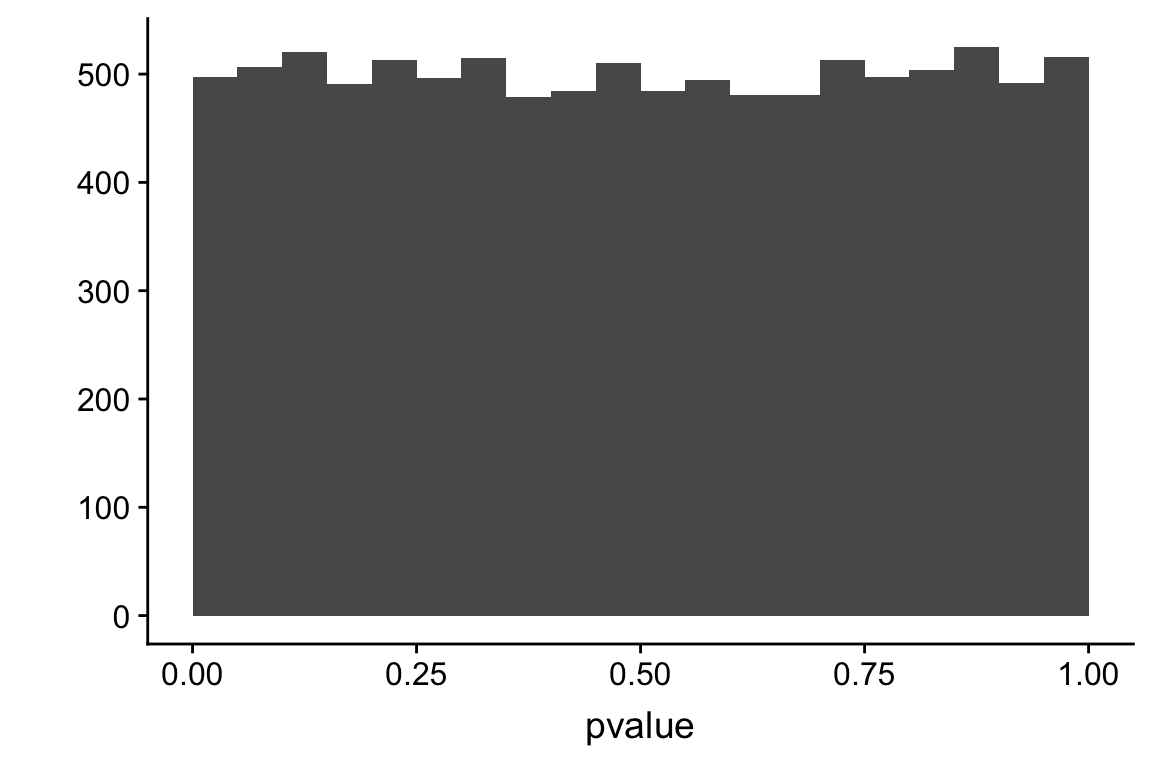
\includegraphics{Walker-elementary-statistical-modeling-draft_files/figure-latex/uniform-1.pdf}

\textbf{The incredible inconsistency of the \(p\)-value}

How replicable is the conclusion of an experiment if the \(p\)-value for
a \(t\)-test is 0.03? If our conclusion is based on \(p < 0.05\), then
the conclusion is not very replicable. The simulation below shows the
results of 15 replicates of an experiment with true power of 40\%. There
are five ``significant'' results (one less than expected) but several
replicates have very high \(p\)-values.

\begin{figure}
\centering
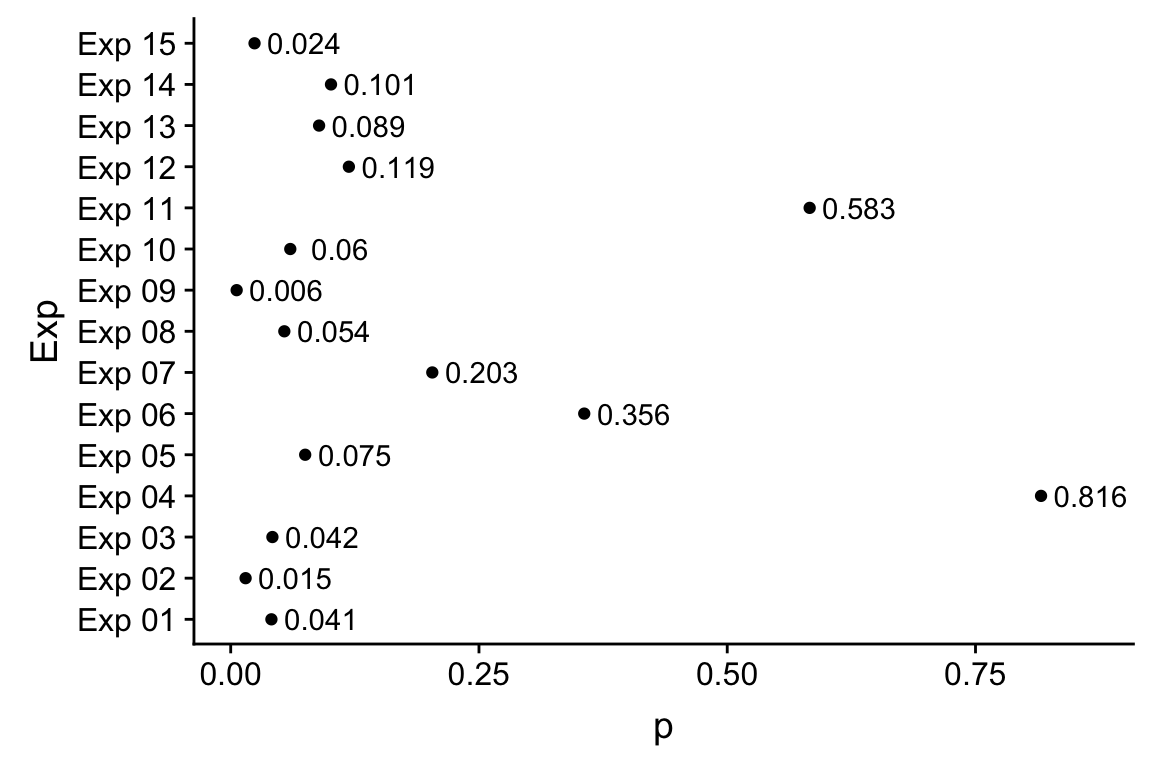
\includegraphics{Walker-elementary-statistical-modeling-draft_files/figure-latex/dance-fig-1.pdf}
\caption{\label{fig:dance-fig}Variability of \(p\)-values when the power is
0.4}
\end{figure}

\subsubsection{Misconception: 0.05 is the lifetime rate of false
discoveries}\label{misconception-0.05-is-the-lifetime-rate-of-false-discoveries}

An important and widespread misconception is that if a researcher
consistently uses \(\alpha=0.05\), then the frequency of incorrectly
concluding an effect exists, or ``discovering'' an effect, over the
lifetime of the researcher, will be 5\%. This is incorrect. This ``false
discovery rate'' is the frequency of false positives divided by the
frequency of positives (the sum of false and true positives). This
differs from the the Type I error rate, which is the frequency of false
positives divided by the frequency of tests \emph{in which the null is
true}.

Imagine we test

\begin{enumerate}
\def\labelenumi{\arabic{enumi}.}
\tightlist
\item
  1000 null hypotheses over a lifetime
\item
  60\% are true nulls, this means there are 600 true nulls and 400 true
  effects
\item
  alpha is 5\%. This means we expect to find \(p \le 0.05\) 30 times
  (\(0.05 \times 600\)) when the null is true
\item
  power is 25\%. This means we expect to find \(p \le 0.05\) 100 times
  (\(0.25 \times 400\)) when the null is false
\item
  We have made \(30 + 100=130\) ``discoveries'' (all experiments with
  \(p \le 0.05\)), but
\item
  30 of the 130, or 23\%, are ``false discoveries''.
\end{enumerate}

That is 11.7\% is the ``false discovery rate''.

Think about this. If the null is never true, you cannot have a false
discovery--every \(p \le 0.05\) is a true discovery (the false discovery
rate is 0\%). And if the null is always true, every \(p < 0.05\) is a
false discovery (the false discovery rate is 100\%).

\subsubsection{\texorpdfstring{Misconception: a low \(p\)-value
indicates an important
effect}{Misconception: a low p-value indicates an important effect}}\label{misconception-a-low-p-value-indicates-an-important-effect}

Many researchers write results as if they believe that a small
\(p\)-value means the effect is big or important. This may misconception
may arise because of the ubiquitous use of ``significant'' to indicate a
small p-value and ``very'' or ``extremely'' or ``wicked'' significant to
indicate a really small p-value. Regardless, this is a misconception. A
small p-value will usually result when there is high power (but can
occur even if power is low) and power is a function of effect size,
variability (the standard deviation), and sample size. A small \(p\)
could result from a large effect size but can also result with a small
effect size if the sample size is big enough.

This is easy to simulate (see script below). Let's model the effect of
the genotype of a gene on height

\begin{Shaded}
\begin{Highlighting}[]
\KeywordTok{set.seed}\NormalTok{(}\DecValTok{1}\NormalTok{)}
\NormalTok{rho <-}\StringTok{ }\FloatTok{0.5}
\NormalTok{n <-}\StringTok{ }\DecValTok{10}\OperatorTok{^}\DecValTok{4}
\NormalTok{genotype <-}\StringTok{ }\KeywordTok{c}\NormalTok{(}\StringTok{"+/+"}\NormalTok{, }\StringTok{"+/-"}\NormalTok{, }\StringTok{"-/-"}\NormalTok{)}
\NormalTok{Sigma <-}\StringTok{ }\KeywordTok{diag}\NormalTok{(}\DecValTok{2}\NormalTok{)}
\NormalTok{Sigma[}\DecValTok{1}\NormalTok{,}\DecValTok{2}\NormalTok{] <-}\StringTok{ }\NormalTok{Sigma[}\DecValTok{2}\NormalTok{,}\DecValTok{1}\NormalTok{] <-}\StringTok{ }\NormalTok{rho}
\NormalTok{X <-}\StringTok{ }\KeywordTok{rmvnorm}\NormalTok{(n, }\DataTypeTok{mean=}\KeywordTok{c}\NormalTok{(}\DecValTok{0}\NormalTok{,}\DecValTok{0}\NormalTok{), }\DataTypeTok{sigma=}\NormalTok{Sigma)}
\KeywordTok{colnames}\NormalTok{(X) <-}\StringTok{ }\KeywordTok{c}\NormalTok{(}\StringTok{"X1"}\NormalTok{, }\StringTok{"X2"}\NormalTok{)}
\NormalTok{beta <-}\StringTok{ }\KeywordTok{c}\NormalTok{(}\FloatTok{0.05}\NormalTok{, }\FloatTok{0.05}\NormalTok{)}
\NormalTok{y <-}\StringTok{ }\NormalTok{X}\OperatorTok\NormalTok{beta }\OperatorTok{+}\StringTok{ }\KeywordTok{rnorm}\NormalTok{(n)}
\NormalTok{fit <-}\StringTok{ }\KeywordTok{lm}\NormalTok{(y }\OperatorTok{~}\StringTok{ }\NormalTok{X)}
\KeywordTok{coefficients}\NormalTok{(}\KeywordTok{summary}\NormalTok{(fit))}
\end{Highlighting}
\end{Shaded}

\begin{verbatim}
##                Estimate Std. Error   t value     Pr(>|t|)
## (Intercept) 0.007472959 0.01007946 0.7414046 4.584656e-01
## XX1         0.044304824 0.01154709 3.8368830 1.253725e-04
## XX2         0.048228101 0.01170855 4.1190490 3.835033e-05
\end{verbatim}

\subsubsection{\texorpdfstring{Misconception: a low \(p\)-value
indicates high model fit or high predictive
capacity}{Misconception: a low p-value indicates high model fit or high predictive capacity}}\label{misconception-a-low-p-value-indicates-high-model-fit-or-high-predictive-capacity}

On page 606, of Lock et al ``Statistics: Unlocking the Power of Data'',
the authors state in item D ``The p-value from the ANOVA table is 0.000
so the model as a whole is effective at predicting grade point
averages.'' This is incorrect. A p-value is not a measure of the
predictive capacity of a model because the p-value is a function of 1)
signal, 2) noise (unmodeled error), and 3) sample size while predictive
capacity is a function of the signal:noise ratio. If the signal:noise
ratio is tiny, the predictive capacity is small but the p-value can be
tiny if the sample size is large. This is easy to simulate (see script
below). The whole-model p-value is exceptionally small (0.00001002) but
the relative predictive ability, measured by the \(R^2\), is near zero
(0.002).

\begin{Shaded}
\begin{Highlighting}[]
\KeywordTok{set.seed}\NormalTok{(}\DecValTok{1}\NormalTok{)}
\NormalTok{rho <-}\StringTok{ }\FloatTok{0.5}
\NormalTok{n <-}\StringTok{ }\DecValTok{10}\OperatorTok{^}\DecValTok{4}
\NormalTok{Sigma <-}\StringTok{ }\KeywordTok{diag}\NormalTok{(}\DecValTok{2}\NormalTok{)}
\NormalTok{Sigma[}\DecValTok{1}\NormalTok{,}\DecValTok{2}\NormalTok{] <-}\StringTok{ }\NormalTok{Sigma[}\DecValTok{2}\NormalTok{,}\DecValTok{1}\NormalTok{] <-}\StringTok{ }\NormalTok{rho}
\NormalTok{X <-}\StringTok{ }\KeywordTok{rmvnorm}\NormalTok{(n, }\DataTypeTok{mean=}\KeywordTok{c}\NormalTok{(}\DecValTok{0}\NormalTok{,}\DecValTok{0}\NormalTok{), }\DataTypeTok{sigma=}\NormalTok{Sigma)}
\KeywordTok{colnames}\NormalTok{(X) <-}\StringTok{ }\KeywordTok{c}\NormalTok{(}\StringTok{"X1"}\NormalTok{, }\StringTok{"X2"}\NormalTok{)}
\NormalTok{beta <-}\StringTok{ }\KeywordTok{c}\NormalTok{(}\FloatTok{0.05}\NormalTok{, }\OperatorTok{-}\FloatTok{0.05}\NormalTok{)}
\NormalTok{y <-}\StringTok{ }\NormalTok{X}\OperatorTok\NormalTok{beta }\OperatorTok{+}\StringTok{ }\KeywordTok{rnorm}\NormalTok{(n)}
\NormalTok{fit <-}\StringTok{ }\KeywordTok{lm}\NormalTok{(y }\OperatorTok{~}\StringTok{ }\NormalTok{X)}
\KeywordTok{summary}\NormalTok{(fit)}
\end{Highlighting}
\end{Shaded}

\begin{verbatim}
## 
## Call:
## lm(formula = y ~ X)
## 
## Residuals:
##     Min      1Q  Median      3Q     Max 
## -3.6449 -0.6857  0.0148  0.6756  3.6510 
## 
## Coefficients:
##              Estimate Std. Error t value Pr(>|t|)    
## (Intercept)  0.007473   0.010079   0.741 0.458466    
## XX1          0.044305   0.011547   3.837 0.000125 ***
## XX2         -0.051772   0.011709  -4.422  9.9e-06 ***
## ---
## Signif. codes:  0 '***' 0.001 '**' 0.01 '*' 0.05 '.' 0.1 ' ' 1
## 
## Residual standard error: 1.008 on 9997 degrees of freedom
## Multiple R-squared:  0.0023, Adjusted R-squared:  0.002101 
## F-statistic: 11.52 on 2 and 9997 DF,  p-value: 1.002e-05
\end{verbatim}

\paragraph{\texorpdfstring{What the \(p\)-value does not
mean}{What the p-value does not mean}}\label{what-the-p-value-does-not-mean}

\begin{enumerate}
\def\labelenumi{\arabic{enumi}.}
\tightlist
\item
  \(p\) is not the probability of the null being true. More formally,
  this probability is \(P(null | data)\) but our \(p\)-value is
  \(P(data | null)\). These are not the same. \(P(null | data)\) is the
  probability of the null being true given the data. \(P(data | null)\)
  is the probability of our data, or something more extreme than our
  data, conditional on a true null.
\item
  \(1-p\) is not the probability of the alternative
\item
  \(p\) is not a measure of effect size.
\item
  \(p\) in one experiment is not the same level of evidence against the
  null as in another experiment
\item
  \(p\) is not a great indicator of which is more likely, H0 or H1.
\item
  If one treatment level has \(p < 0.05\) and another treatment level
  has \(p > 0.05\), this is not evidence that the treatment levels have
  different effects on the outcome.
\end{enumerate}

\subsection{Recommendations}\label{recommendations}

\textbf{If you are working on basic science research} simply report the
exact \(p\)-value, along with a CI. If \(p < 0.05\) (or some other
\(\alpha\)) do not report this as ``significant'' -- in fact, avoid the
word ``significant''. In the english language, ``significant'' implies
big or important. Small \(p\)-values can result even with trivially
small effects if \(n\) is big or sample variation is small. If \(p\) is
smaller than say 0.001, then this is pretty good evidence that the data
is not a fluke of sampling. But if \(p\) is closer to 0.01 or 0.05, this
is only weak evidence of a fluke because of the sampling variability of
\(p\).

\textbf{If you are working on quality control} then a \(p\) value is a
useful tool, but is only relevant compared to a decision rule with
well-reasoned values of \(\alpha\) and \(\beta\) -- exact values of
\(p\) are not very meaningful.

\section{Problems}\label{problems-1}

Problem 1 -- simulate the distribution of \(p\) under the null. There
are many ways to do this but a straightforard approach is to

\begin{enumerate}
\def\labelenumi{\arabic{enumi}.}
\tightlist
\item
  Create a \(2n \times m\) matrix of random normal deviates with mean 0
  and sd 1
\item
  Do a \(t\)-test on each column, with the first \(n\) values assigned
  to one group and the remaining \(n\) values assigned to the second
  group. Save the \(p\)-value from each.
\item
  Plot a histogram of the \(p\)-values.
\item
  What is the distribution? What is the most likely value of \(p\)?
\end{enumerate}

Problem 2 -- simulate power. Again, many ways to do this but following
up on Problem 1. 1. Create a \(2n \times m\) matrix of random normal
deviates with mean 0 and sd 1 2. Add an effect to the first \(n\) values
of each column. Things to think about a. what is a good effect size to
add? The effect/sd ratio, known as Cohen's d, is a relative (or
standardized) measure of effect size. Cohen suggest 0.2, 0.5, and 0.8 as
small, medium, and large standardized effects. b. should the same effect
be added to each individual? Yes! It is the random component that
captures the individual variation in the response. 3. Do a \(t\)-test on
each column of the matrix, using the first \(n\) values in group 1 and
the remaining \(n\) values in group 2. Save the p-values for each. 4.
Compute the power, the relative frequency \(p \le 0.05\). 5. Repeat with
different values of \(n\), effect size, and sd, but only vary one at a
time. How does power vary with these three parameters?

Problem 3 -- write a script for a permutation test of the vitamin E and
vitamin C levels of the vole data. Compare this to the \(t\)-test.

Problem 4 -- grad students only. Simulate the false discovery rate.
Explore the parameters: the frequency of true nulls and the power.

\chapter{Creating Fake Data}\label{creating-fake-data}

Fake data are generated by sampling from one of R's random sampling
functions. These functions sample from different distributions including

\begin{enumerate}
\def\labelenumi{\arabic{enumi}.}
\tightlist
\item
  uniform -- function \texttt{runif(n,\ min=0,\ max=1)}, which samples n
  continous values between \texttt{min} and \texttt{max}.
\item
  normal (Gaussian) -- function \texttt{rnorm(n,\ mean=0,\ sd=1)}, which
  samples n continous values from a distribution with the specified mean
  and standard deviation. The default is the ``standard'' normal
  distribution.
\item
  poisson -- function \texttt{rpois(n,\ lambda)}, which samples
  \texttt{n} counts from a distribution with mean and variance equal to
  \texttt{lambda}.
\item
  negative binomial -- \texttt{rnegbin(n,\ mu=n,\ theta)}, which samples
  \texttt{n} counts with mean \texttt{mu} and variance
  \texttt{mu\ +\ mu\^{}2/theta}.
\end{enumerate}

\subsection{Continuous X (fake observational
data)}\label{continuous-x-fake-observational-data}

A very simple simulation of observational design (the \(X\) are not at
``controlled'' levels)

\begin{Shaded}
\begin{Highlighting}[]
\NormalTok{n <-}\StringTok{ }\DecValTok{25}
\CommentTok{# the paramters}
\NormalTok{beta_}\DecValTok{0}\NormalTok{ <-}\StringTok{ }\DecValTok{25} \CommentTok{# the true intercept}
\NormalTok{beta_}\DecValTok{1}\NormalTok{ <-}\StringTok{ }\FloatTok{3.4} \CommentTok{# the true slope}
\NormalTok{sigma <-}\StringTok{ }\DecValTok{2} \CommentTok{# the true standard deviation}

\NormalTok{x <-}\StringTok{ }\KeywordTok{rnorm}\NormalTok{(n)}
\NormalTok{y <-}\StringTok{ }\NormalTok{beta_}\DecValTok{0} \OperatorTok{+}\StringTok{ }\NormalTok{beta_}\DecValTok{1}\OperatorTok{*}\NormalTok{x }\OperatorTok{+}\StringTok{ }\KeywordTok{rnorm}\NormalTok{(n, }\DataTypeTok{sd=}\NormalTok{sigma)}
\KeywordTok{qplot}\NormalTok{(x, y)}
\end{Highlighting}
\end{Shaded}

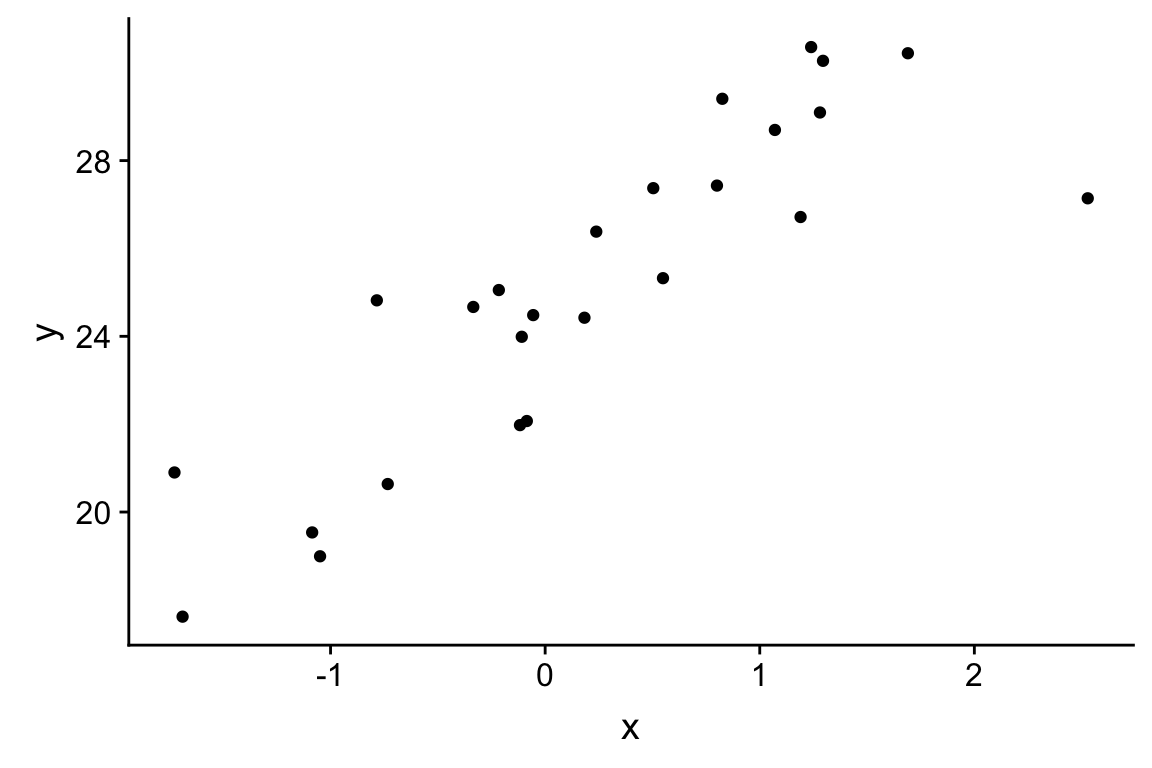
\includegraphics{Walker-elementary-statistical-modeling-draft_files/figure-latex/continuous-X-1.pdf}

How well does a model fit to the data recover the true parameters?

\begin{Shaded}
\begin{Highlighting}[]
\NormalTok{fit <-}\StringTok{ }\KeywordTok{lm}\NormalTok{(y }\OperatorTok{~}\StringTok{ }\NormalTok{x)}
\NormalTok{knitr}\OperatorTok{::}\KeywordTok{kable}\NormalTok{(}\KeywordTok{coefficients}\NormalTok{(}\KeywordTok{summary}\NormalTok{(fit)), }\DataTypeTok{digits=}\KeywordTok{c}\NormalTok{(}\DecValTok{1}\NormalTok{, }\DecValTok{2}\NormalTok{, }\DecValTok{1}\NormalTok{, }\DecValTok{4}\NormalTok{))}
\end{Highlighting}
\end{Shaded}

\begin{tabular}{l|r|r|r|r}
\hline
  & Estimate & Std. Error & t value & Pr(>|t|)\\
\hline
(Intercept) & 25.8 & 0.34 & 75.8 & 0\\
\hline
x & 4.2 & 0.40 & 10.4 & 0\\
\hline
\end{tabular}

The coefficient of \(x\) is the ``Estimate''. How close is the estimate?
Run the simulation several times to look at the variation in the
estimate -- this will give you a sense of the uncertainty. Increase
\(n\) and explore this uncertainty. Increase all the way up to
\(n=10^5\). Commenting out the qplot line will make this exploration
easier.

\subsection{Categorical X (fake experimental
data)}\label{categorical-x-fake-experimental-data}

Similar to above but the \(X\) are at controlled levels and so this
simulates an experimental design

\begin{Shaded}
\begin{Highlighting}[]
\NormalTok{n <-}\StringTok{ }\DecValTok{5} \CommentTok{# the sample size per treatment level}

\NormalTok{fake_data <-}\StringTok{ }\KeywordTok{data.table}\NormalTok{(}\DataTypeTok{Treatment=}\KeywordTok{rep}\NormalTok{(}\KeywordTok{c}\NormalTok{(}\StringTok{"control"}\NormalTok{, }\StringTok{"treated"}\NormalTok{), }\DataTypeTok{each=}\NormalTok{n))}
\NormalTok{beta_}\DecValTok{0}\NormalTok{ <-}\StringTok{ }\FloatTok{10.5} \CommentTok{# mean of untreated}
\NormalTok{beta_}\DecValTok{1}\NormalTok{ <-}\StringTok{ }\FloatTok{2.1} \CommentTok{# difference in means (treated - untreated)}
\NormalTok{sigma <-}\StringTok{ }\DecValTok{3} \CommentTok{# the error standard deviation}
\CommentTok{# the Y variable ("Response") is a function of treatment. We use some matrix}
\CommentTok{# algebra to get this done.}
\CommentTok{# Turn the Treatment assignment into a model matrix. Take a peak at X!}
\NormalTok{X <-}\StringTok{ }\KeywordTok{model.matrix}\NormalTok{(}\OperatorTok{~}\StringTok{ }\NormalTok{Treatment, fake_data)}
\CommentTok{# to make the math easier the coefficients are collected into a vector}
\NormalTok{beta <-}\StringTok{ }\KeywordTok{c}\NormalTok{(beta_}\DecValTok{0}\NormalTok{, beta_}\DecValTok{1}\NormalTok{)}
\CommentTok{# you will see the formula Y=Xb many times. Here it is coded in R}
\NormalTok{fake_data[, Response}\OperatorTok{:}\ErrorTok{=}\NormalTok{X}\OperatorTok\NormalTok{beta }\OperatorTok{+}\StringTok{ }\KeywordTok{rnorm}\NormalTok{(n, }\DataTypeTok{sd=}\NormalTok{sigma)]}
\CommentTok{# plot it with a strip chart (often called a "dot plot")}
\KeywordTok{ggstripchart}\NormalTok{(}\DataTypeTok{data=}\NormalTok{fake_data, }\DataTypeTok{x=}\StringTok{"Treatment"}\NormalTok{, }\DataTypeTok{y=}\StringTok{"Response"}\NormalTok{, }\DataTypeTok{add =} \KeywordTok{c}\NormalTok{(}\StringTok{"mean_se"}\NormalTok{))}
\end{Highlighting}
\end{Shaded}

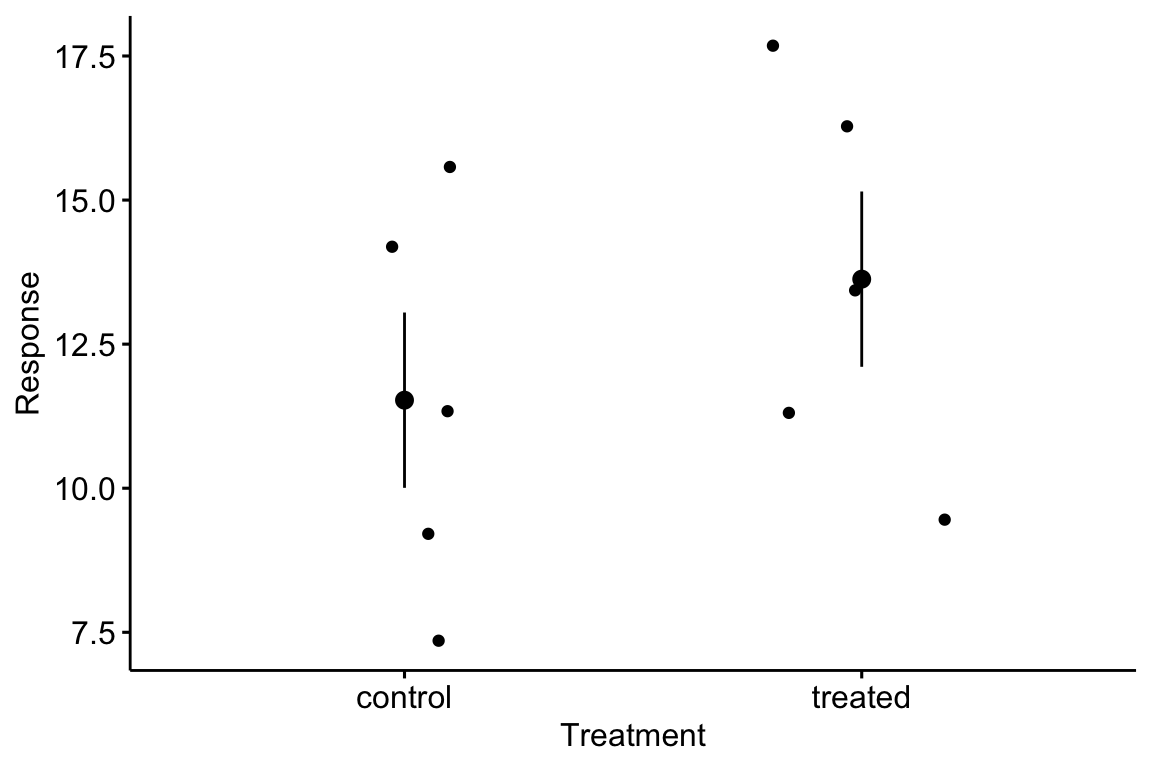
\includegraphics{Walker-elementary-statistical-modeling-draft_files/figure-latex/categorical-X-1.pdf}

\begin{Shaded}
\begin{Highlighting}[]
\CommentTok{# fit using base R linear model function}
\NormalTok{fit <-}\StringTok{ }\KeywordTok{lm}\NormalTok{(Response }\OperatorTok{~}\StringTok{ }\NormalTok{Treatment, }\DataTypeTok{data=}\NormalTok{fake_data)}
\CommentTok{# display a pretty table of the coefficients}
\NormalTok{knitr}\OperatorTok{::}\KeywordTok{kable}\NormalTok{(}\KeywordTok{coefficients}\NormalTok{(}\KeywordTok{summary}\NormalTok{(fit)), }\DataTypeTok{digits=}\DecValTok{3}\NormalTok{)}
\end{Highlighting}
\end{Shaded}

\begin{tabular}{l|r|r|r|r}
\hline
  & Estimate & Std. Error & t value & Pr(>|t|)\\
\hline
(Intercept) & 11.626 & 1.097 & 10.601 & 0.000\\
\hline
Treatmenttreated & 2.100 & 1.551 & 1.354 & 0.213\\
\hline
\end{tabular}

Check that the intercept is close to beta\_0 and the coefficient for
Treatment is close to beta\_1. This coefficient is the difference in
means between the treatment levels. It is the simulated effect. Again,
change \(n\). Good values are \(n=20\) and \(n=100\). Again, comment out
the plot line to make exploration more efficient.

\subsection{Correlated X (fake observational
data)}\label{correlated-x-fake-observational-data}

\subsubsection{Generating correlated X
variables}\label{generating-correlated-x-variables}

It's useful to think about how correlated data are generated because
often we want to generate fake\_data with an expected correlation. Let's
say we want to generate two X variables that have an expected
correlation of 0.6. To generate this, we take advantage of the fact that
two variables, X1 and X2, are correlated if they share a ``common
cause'' -- a variable Z that effects (or ``causes'') both X1 and X2. If
the expected variances of X1, X2, and Z are all 1, then the expected
correlation between X1 and X2 is the product of the causal effect from Z
to each X. The easiest way to implement this is to simply make the
effect from Z to both X equal to \(\sqrt(0.6)\).

\begin{Shaded}
\begin{Highlighting}[]
\NormalTok{n <-}\StringTok{ }\DecValTok{10}\OperatorTok{^}\DecValTok{3}
\NormalTok{z <-}\StringTok{ }\KeywordTok{rnorm}\NormalTok{(n) }\CommentTok{# the common cause, with sigma = 1}
\NormalTok{rho <-}\StringTok{ }\FloatTok{0.6} \CommentTok{# the true correlation between X1 and X2}
\NormalTok{beta_z <-}\StringTok{ }\KeywordTok{sqrt}\NormalTok{(rho) }\CommentTok{# the easiest way to get effects of z on X1 and X2 that generates rho}
\NormalTok{sigma_x <-}\StringTok{ }\KeywordTok{sqrt}\NormalTok{(}\DecValTok{1} \OperatorTok{-}\StringTok{ }\NormalTok{rho) }\CommentTok{# we will make the variance of X1 and X2 = 1, so the "explained" variance in X is beta_z^2 = rho so this is the sqrt of the unexplained variance}
\NormalTok{x1 <-}\StringTok{ }\NormalTok{beta_z}\OperatorTok{*}\NormalTok{z }\OperatorTok{+}\StringTok{ }\KeywordTok{rnorm}\NormalTok{(n, }\DataTypeTok{sd=}\NormalTok{sigma_x)}
\NormalTok{x2 <-}\StringTok{ }\NormalTok{beta_z}\OperatorTok{*}\NormalTok{z }\OperatorTok{+}\StringTok{ }\KeywordTok{rnorm}\NormalTok{(n, }\DataTypeTok{sd=}\NormalTok{sigma_x)}
\CommentTok{# check}
\KeywordTok{cov}\NormalTok{(}\KeywordTok{data.frame}\NormalTok{(}\DataTypeTok{X1=}\NormalTok{x1, }\DataTypeTok{X2=}\NormalTok{x2)) }\CommentTok{# is the diagonal close to 1, 1?}
\end{Highlighting}
\end{Shaded}

\begin{verbatim}
##           X1        X2
## X1 1.0523598 0.5978408
## X2 0.5978408 0.9713292
\end{verbatim}

\begin{Shaded}
\begin{Highlighting}[]
\KeywordTok{cor}\NormalTok{(x1, x2) }\CommentTok{# is the value close to rho?}
\end{Highlighting}
\end{Shaded}

\begin{verbatim}
## [1] 0.5913168
\end{verbatim}

\begin{Shaded}
\begin{Highlighting}[]
\KeywordTok{qplot}\NormalTok{(x1, x2)}
\end{Highlighting}
\end{Shaded}

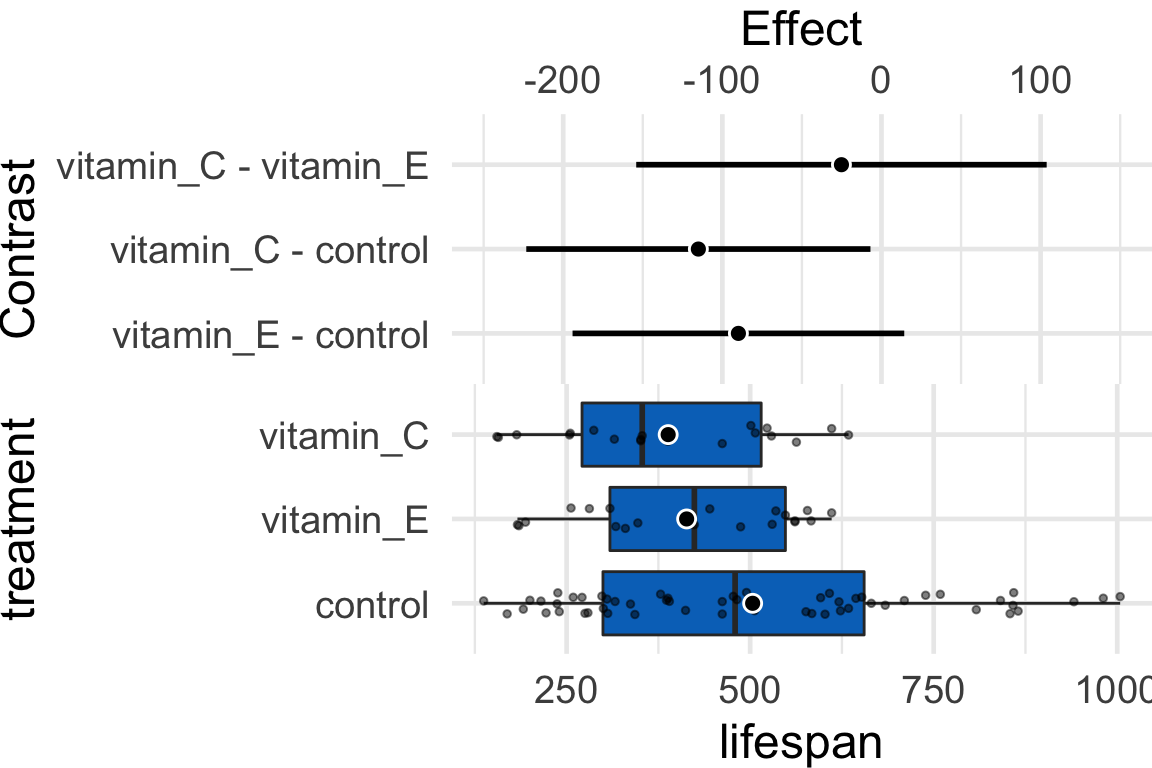
\includegraphics{Walker-elementary-statistical-modeling-draft_files/figure-latex/unnamed-chunk-13-1.pdf}

Now create fake \(Y\) that is a function of both \(X_1\) and \(X_2\).
Create ``standardized'' fake data, where \(\sigma_Y = 1\).

\begin{Shaded}
\begin{Highlighting}[]
\NormalTok{beta_}\DecValTok{0}\NormalTok{ <-}\StringTok{ }\FloatTok{3.2}
\NormalTok{beta_}\DecValTok{1}\NormalTok{ <-}\StringTok{ }\FloatTok{0.7}
\NormalTok{beta_}\DecValTok{2}\NormalTok{ <-}\StringTok{ }\OperatorTok{-}\FloatTok{0.3}
\NormalTok{explained_sigma <-}\StringTok{ }\NormalTok{beta_}\DecValTok{1}\OperatorTok{^}\DecValTok{2} \OperatorTok{+}\StringTok{ }\NormalTok{beta_}\DecValTok{2}\OperatorTok{^}\DecValTok{2} \OperatorTok{+}\StringTok{ }\DecValTok{2}\OperatorTok{*}\NormalTok{beta_}\DecValTok{1}\OperatorTok{*}\NormalTok{beta_}\DecValTok{2}\OperatorTok{*}\NormalTok{rho }\CommentTok{# Wright's rules! Compare to Trig!}
\NormalTok{sigma_Y.X <-}\StringTok{ }\KeywordTok{sqrt}\NormalTok{(}\DecValTok{1} \OperatorTok{-}\StringTok{ }\NormalTok{explained_sigma) }\CommentTok{# sqrt unexplained variance}
\NormalTok{y <-}\StringTok{ }\NormalTok{beta_}\DecValTok{0} \OperatorTok{+}\StringTok{ }\NormalTok{beta_}\DecValTok{1}\OperatorTok{*}\NormalTok{x1 }\OperatorTok{+}\StringTok{ }\NormalTok{beta_}\DecValTok{2}\OperatorTok{*}\NormalTok{x2 }\OperatorTok{+}\StringTok{ }\KeywordTok{rnorm}\NormalTok{(n, }\DataTypeTok{sd=}\NormalTok{sigma_Y.X)}

\CommentTok{# check}
\KeywordTok{var}\NormalTok{(y) }\CommentTok{# should be close to 1 as n gets bigger}
\end{Highlighting}
\end{Shaded}

\begin{verbatim}
## [1] 0.9791502
\end{verbatim}

\begin{Shaded}
\begin{Highlighting}[]
\CommentTok{# check parameters}
\KeywordTok{coef}\NormalTok{(}\KeywordTok{summary}\NormalTok{(}\KeywordTok{lm}\NormalTok{(y }\OperatorTok{~}\StringTok{ }\NormalTok{x1 }\OperatorTok{+}\StringTok{ }\NormalTok{x2))) }\CommentTok{# should be near parameters as n gets bigger}
\end{Highlighting}
\end{Shaded}

\begin{verbatim}
##               Estimate Std. Error    t value     Pr(>|t|)
## (Intercept)  3.1887712 0.02536483 125.716255 0.000000e+00
## x1           0.6885565 0.03064195  22.471043 8.422461e-91
## x2          -0.3037457 0.03189446  -9.523465 1.223898e-20
\end{verbatim}

Note that the variance of \(Y\) is the variance of the explained part
due to X1 and X2 and the unexplained part and if the expected variance
of \(Y=1\) then this sets an upper limit for the explained part. This
means that

\begin{equation}
\beta_1^2 + \beta_2^2 + 2 \beta_1 \beta_2 \rho < 1
\end{equation}

which means the magnitude of \(\beta_1\) and \(\beta_2\) should
generally be less than 1.

\subsubsection{Creating mulitple X variables using the package
mvtnorm}\label{creating-mulitple-x-variables-using-the-package-mvtnorm}

The package mvtnorm provides a function to generate multivariate data
(multiple columns) with a specified vector of means (the means of each
column) and covariance matrix among the means.

\begin{Shaded}
\begin{Highlighting}[]
\NormalTok{rcov1 <-}\StringTok{ }\ControlFlowTok{function}\NormalTok{(p)\{}
  \CommentTok{# p is the number of columns or number of variables}
\NormalTok{  pp <-}\StringTok{ }\NormalTok{p}\OperatorTok{*}\NormalTok{(p}\OperatorTok{-}\DecValTok{1}\NormalTok{)}\OperatorTok{/}\DecValTok{2} \CommentTok{# number of elements in lower tri}
\NormalTok{  max_r <-}\StringTok{ }\FloatTok{0.7}
\NormalTok{  r <-}\StringTok{ }\KeywordTok{rexp}\NormalTok{(pp)}
\NormalTok{  r <-}\StringTok{ }\NormalTok{r}\OperatorTok{*}\NormalTok{max_r}\OperatorTok{/}\KeywordTok{max}\NormalTok{(r)}
  
  \CommentTok{# create correlation matrix}
\NormalTok{  R <-}\StringTok{ }\KeywordTok{matrix}\NormalTok{(}\DecValTok{1}\NormalTok{, }\DataTypeTok{nrow=}\NormalTok{p, }\DataTypeTok{ncol=}\NormalTok{p)}
\NormalTok{  R[}\KeywordTok{lower.tri}\NormalTok{(R, }\DataTypeTok{diag=}\OtherTok{FALSE}\NormalTok{)] <-}\StringTok{ }\NormalTok{r}
\NormalTok{  R <-}\StringTok{ }\KeywordTok{t}\NormalTok{(R)}
\NormalTok{  R[}\KeywordTok{lower.tri}\NormalTok{(R, }\DataTypeTok{diag=}\OtherTok{FALSE}\NormalTok{)] <-}\StringTok{ }\NormalTok{r}
  
  \CommentTok{# convert to covariance matrix}
\NormalTok{  L <-}\StringTok{ }\KeywordTok{diag}\NormalTok{(}\KeywordTok{sqrt}\NormalTok{(}\KeywordTok{rexp}\NormalTok{(p))) }\CommentTok{# standard deviations}
\NormalTok{  S <-}\StringTok{ }\NormalTok{L}\OperatorTok\NormalTok{R}\OperatorTok\NormalTok{L}
  
  \CommentTok{# check -- these should be the same}
  \CommentTok{# R}
  \CommentTok{# cov2cor(S)}
  \KeywordTok{return}\NormalTok{(S)}
\NormalTok{\}}
\end{Highlighting}
\end{Shaded}

Now let's use mvtnorm to generate fake correlated X

\begin{Shaded}
\begin{Highlighting}[]
\NormalTok{p <-}\StringTok{ }\DecValTok{5} \CommentTok{# number of X variables}
\NormalTok{S <-}\StringTok{ }\KeywordTok{rcov1}\NormalTok{(p)}

\CommentTok{# make the fake X}
\NormalTok{n <-}\StringTok{ }\DecValTok{10}\OperatorTok{^}\DecValTok{5}
\NormalTok{mu <-}\StringTok{ }\KeywordTok{runif}\NormalTok{(p, }\DataTypeTok{min=}\DecValTok{10}\NormalTok{, }\DataTypeTok{max=}\DecValTok{100}\NormalTok{) }\CommentTok{# vecctor of p means}
\NormalTok{X <-}\StringTok{ }\KeywordTok{rmvnorm}\NormalTok{(n, }\DataTypeTok{mean=}\NormalTok{mu, }\DataTypeTok{sigma=}\NormalTok{S)}

\CommentTok{# how close? (check the cor as this is easier to scan)}
\KeywordTok{cov2cor}\NormalTok{(S)}
\end{Highlighting}
\end{Shaded}

\begin{verbatim}
##           [,1]       [,2]       [,3]       [,4]       [,5]
## [1,] 1.0000000 0.15511020 0.11863165 0.48788949 0.14545246
## [2,] 0.1551102 1.00000000 0.70000000 0.03514487 0.04345391
## [3,] 0.1186317 0.70000000 1.00000000 0.05346376 0.54083807
## [4,] 0.4878895 0.03514487 0.05346376 1.00000000 0.44504979
## [5,] 0.1454525 0.04345391 0.54083807 0.44504979 1.00000000
\end{verbatim}

\begin{Shaded}
\begin{Highlighting}[]
\KeywordTok{cor}\NormalTok{(X)}
\end{Highlighting}
\end{Shaded}

\begin{verbatim}
##           [,1]       [,2]       [,3]       [,4]       [,5]
## [1,] 1.0000000 0.15618693 0.12146387 0.48987841 0.14569745
## [2,] 0.1561869 1.00000000 0.69709529 0.03879653 0.03961509
## [3,] 0.1214639 0.69709529 1.00000000 0.05598629 0.54138395
## [4,] 0.4898784 0.03879653 0.05598629 1.00000000 0.44214983
## [5,] 0.1456974 0.03961509 0.54138395 0.44214983 1.00000000
\end{verbatim}

\subsubsection{The rcov1 algorithm is
naive}\label{the-rcov1-algorithm-is-naive}

A problem with generating a fake covariance matrix as above is that it
is likely to be \textbf{singular} as \(p\) get's bigger. A singular
covariance matrix is one where there are fewer orthogonal axes of
variation then there are variables. Imagine a multidimensional
scatterplot of a data set with the fake covariance matrix. If we zoom
around this multidimensional space, we will come across a ``view'' in
which all the points are compressed along a single line -- that is there
is no variation on the axis orthogonal to this line of points. This is
bad, as it means we cannot fit a linear model using least squares
(because the inverse of the covariance matrix doesn't exist).

Let's explore this. If the a covariance matrix is singular, then at
least one eigenvalue of the matrix is negative (eigenvalues is a
multivariate term beyond the scope of this text but, effectively, these
are the variances of the orthogonal axes referred to above). Here I
compute the frequency of covariance matrices with at least one negative
eigenvalue as \(p\) increases

\begin{Shaded}
\begin{Highlighting}[]
\NormalTok{niter <-}\StringTok{ }\DecValTok{1000}
\NormalTok{p_vec <-}\StringTok{ }\DecValTok{3}\OperatorTok{:}\DecValTok{10}
\NormalTok{counts <-}\StringTok{ }\KeywordTok{numeric}\NormalTok{(}\KeywordTok{length}\NormalTok{(p_vec))}
\NormalTok{i <-}\StringTok{ }\DecValTok{0}
\ControlFlowTok{for}\NormalTok{(p }\ControlFlowTok{in} \DecValTok{3}\OperatorTok{:}\DecValTok{10}\NormalTok{)\{}
\NormalTok{  i <-}\StringTok{ }\NormalTok{i}\OperatorTok{+}\DecValTok{1}
  \ControlFlowTok{for}\NormalTok{(iter }\ControlFlowTok{in} \DecValTok{1}\OperatorTok{:}\NormalTok{niter)\{}
\NormalTok{    counts[i] <-}\StringTok{ }\KeywordTok{ifelse}\NormalTok{(}\KeywordTok{eigen}\NormalTok{(}\KeywordTok{rcov1}\NormalTok{(p))}\OperatorTok{$}\NormalTok{values[p] }\OperatorTok{<}\StringTok{ }\DecValTok{0}\NormalTok{, counts[i]}\OperatorTok{+}\DecValTok{1}\NormalTok{, counts[i])}
\NormalTok{  \}}
\NormalTok{\}}
\KeywordTok{data.table}\NormalTok{(}\DataTypeTok{p=}\NormalTok{p_vec, }\DataTypeTok{freq=}\NormalTok{counts}\OperatorTok{/}\NormalTok{niter)}
\end{Highlighting}
\end{Shaded}

\begin{verbatim}
##     p  freq
## 1:  3 0.000
## 2:  4 0.025
## 3:  5 0.066
## 4:  6 0.135
## 5:  7 0.190
## 6:  8 0.225
## 7:  9 0.275
## 8: 10 0.368
\end{verbatim}

\subsubsection{Generating multiple columns of X variables with a
non-singular covariance
matrix}\label{generating-multiple-columns-of-x-variables-with-a-non-singular-covariance-matrix}

This section uses some ideas from matrix algebra. The goal is to create
a \(n \times p\) matrix of \(X\) variables that have some random
covariance structure that is full-rank (not singular, or no negative
eigenvalues). The algorithm starts with a \(p \times p\) random
eigenvector matrix \(\mathbf{E}\) and a \(p \times p\) random eigenvalue
matrix \(\mathbf{L}\) and then computes the random covariance matrix
using \(\mathbf{E}\mathbf{L}\mathbf{E}^\top\)

\begin{enumerate}
\def\labelenumi{\arabic{enumi}.}
\tightlist
\item
  Generate a random \(p \times p\) random eigenvector matrix from a
  covariance matrix of \(p \times p\) matrix of random normal variables.
\end{enumerate}

\begin{Shaded}
\begin{Highlighting}[]
\NormalTok{fake.eigenvectors <-}\StringTok{ }\ControlFlowTok{function}\NormalTok{(p)\{}
\NormalTok{    a <-}\StringTok{ }\KeywordTok{matrix}\NormalTok{(}\KeywordTok{rnorm}\NormalTok{(p}\OperatorTok{*}\NormalTok{p), p, p) }\CommentTok{# only orthogonal if p is infinity so need to orthogonalize it}
\NormalTok{    a <-}\StringTok{ }\KeywordTok{t}\NormalTok{(a)}\OperatorTok\NormalTok{a }\CommentTok{# this is the sum-of-squares-and-cross-product-matrix}
\NormalTok{    E <-}\StringTok{ }\KeywordTok{eigen}\NormalTok{(a)}\OperatorTok{$}\NormalTok{vectors }\CommentTok{# decompose to truly orthogonal columns}
    \KeywordTok{return}\NormalTok{(E)}
\NormalTok{\}}
\end{Highlighting}
\end{Shaded}

\begin{enumerate}
\def\labelenumi{\arabic{enumi}.}
\setcounter{enumi}{1}
\tightlist
\item
  Generate \(p\) random eigenvalues in descending order and that sum to
  1. There are several ways to create this sequence. Here are two:
\end{enumerate}

\begin{Shaded}
\begin{Highlighting}[]
\CommentTok{# force the eigenvalues to descend at a constant rate}
\NormalTok{fake.eigenvalues <-}\StringTok{ }\ControlFlowTok{function}\NormalTok{(p, }\DataTypeTok{m=}\NormalTok{p, }\DataTypeTok{start=}\DecValTok{1}\NormalTok{, }\DataTypeTok{rate=}\DecValTok{1}\NormalTok{)\{}
  \CommentTok{# m is the number of positive eigenvalues}
  \CommentTok{# start and rate control the decline in the eigenvalue}
\NormalTok{  s <-}\StringTok{ }\NormalTok{start}\OperatorTok{/}\KeywordTok{seq}\NormalTok{(}\DecValTok{1}\OperatorTok{:}\NormalTok{m)}\OperatorTok{^}\NormalTok{rate}
\NormalTok{  s <-}\StringTok{ }\KeywordTok{c}\NormalTok{(s, }\KeywordTok{rep}\NormalTok{(}\DecValTok{0}\NormalTok{, p}\OperatorTok{-}\NormalTok{m)) }\CommentTok{# add zero eigenvalues}
\NormalTok{  L <-}\StringTok{ }\KeywordTok{diag}\NormalTok{(s}\OperatorTok{/}\KeywordTok{sum}\NormalTok{(s)}\OperatorTok{*}\NormalTok{m) }\CommentTok{# rescale so that sum(s)=m and put into matrix,}
  \CommentTok{# which would occur if all the traits are variance standardized}
  \KeywordTok{return}\NormalTok{(L)}
\NormalTok{\}}

\CommentTok{# random descent}
\NormalTok{fake.eigenvalues.exp <-}\StringTok{ }\ControlFlowTok{function}\NormalTok{(p, }\DataTypeTok{m=}\NormalTok{p, }\DataTypeTok{rate=}\DecValTok{1}\NormalTok{)\{}
  \CommentTok{# exponential distribution of eigenvalues}
  \CommentTok{# m is the number of positive eigenvalues}
  \CommentTok{# start and rate control the decline in the eigenvalue}
\NormalTok{  s <-}\StringTok{ }\KeywordTok{rexp}\NormalTok{(m, rate)}
\NormalTok{  s <-}\StringTok{ }\NormalTok{s[}\KeywordTok{order}\NormalTok{(s, }\DataTypeTok{decreasing=}\OtherTok{TRUE}\NormalTok{)] }\CommentTok{# re-order into descending order}
\NormalTok{  s <-}\StringTok{ }\KeywordTok{c}\NormalTok{(s, }\KeywordTok{rep}\NormalTok{(}\DecValTok{0}\NormalTok{, p}\OperatorTok{-}\NormalTok{m)) }\CommentTok{# add zero eigenvalues}
\NormalTok{  L <-}\StringTok{ }\KeywordTok{diag}\NormalTok{(s}\OperatorTok{/}\KeywordTok{sum}\NormalTok{(s)}\OperatorTok{*}\NormalTok{m) }\CommentTok{# rescale so that sum(s)=m and put into matrix,}
  \CommentTok{# which would occur if all the traits are variance standardized}
  \KeywordTok{return}\NormalTok{(L)}
\NormalTok{\}}
\end{Highlighting}
\end{Shaded}

\begin{enumerate}
\def\labelenumi{\arabic{enumi}.}
\setcounter{enumi}{2}
\tightlist
\item
  Generate the random covariance matrix
\end{enumerate}

\begin{Shaded}
\begin{Highlighting}[]
\NormalTok{fake.cov.matrix <-}\StringTok{ }\ControlFlowTok{function}\NormalTok{(p)\{}
    \CommentTok{# p is the size of the matrix (number of cols and rows)}
\NormalTok{    E <-}\StringTok{ }\KeywordTok{fake.eigenvectors}\NormalTok{(p)}
\NormalTok{    L <-}\StringTok{ }\KeywordTok{diag}\NormalTok{(}\KeywordTok{fake.eigenvalues}\NormalTok{(p))}
\NormalTok{    S <-}\StringTok{ }\NormalTok{E}\OperatorTok\NormalTok{L}\OperatorTok\KeywordTok{t}\NormalTok{(E)}
    \KeywordTok{return}\NormalTok{(S)}
\NormalTok{\}}
\end{Highlighting}
\end{Shaded}

\begin{enumerate}
\def\labelenumi{\arabic{enumi}.}
\setcounter{enumi}{3}
\tightlist
\item
  Generate the random \(X\) variables using
  \(\mathbf{X} = \mathbf{X}' (\mathbf{E}\sqrt{\mathbf{L}})^\top\)
\end{enumerate}

\begin{Shaded}
\begin{Highlighting}[]
\CommentTok{# two functions to compute the random data}
\NormalTok{fake.X <-}\StringTok{ }\ControlFlowTok{function}\NormalTok{(n,p,E,L)\{}
  \CommentTok{# n is number of observations}
  \CommentTok{# p is number of variables}
\NormalTok{  X <-}\StringTok{ }\KeywordTok{matrix}\NormalTok{(}\KeywordTok{rnorm}\NormalTok{(n}\OperatorTok{*}\NormalTok{p),}\DataTypeTok{nrow=}\NormalTok{n,}\DataTypeTok{ncol=}\NormalTok{p) }\OperatorTok\StringTok{ }\KeywordTok{t}\NormalTok{(E}\OperatorTok\KeywordTok{sqrt}\NormalTok{(L))}
    \KeywordTok{return}\NormalTok{(X)}
\NormalTok{\}}
\end{Highlighting}
\end{Shaded}

An example

\begin{Shaded}
\begin{Highlighting}[]
\NormalTok{n <-}\StringTok{ }\DecValTok{10}\OperatorTok{^}\DecValTok{5}
\NormalTok{p <-}\StringTok{ }\DecValTok{5}
\NormalTok{E <-}\StringTok{ }\KeywordTok{fake.eigenvectors}\NormalTok{(p)}
\NormalTok{L <-}\StringTok{ }\KeywordTok{fake.eigenvalues}\NormalTok{(p, }\DataTypeTok{start=}\DecValTok{1}\NormalTok{, }\DataTypeTok{rate=}\DecValTok{1}\NormalTok{)}
\NormalTok{X <-}\StringTok{ }\KeywordTok{fake.X}\NormalTok{(n, p, E, L)}
\KeywordTok{colnames}\NormalTok{(X) <-}\StringTok{ }\KeywordTok{paste0}\NormalTok{(}\StringTok{"X"}\NormalTok{, }\DecValTok{1}\OperatorTok{:}\NormalTok{p)}
\NormalTok{E}
\end{Highlighting}
\end{Shaded}

\begin{verbatim}
##            [,1]        [,2]        [,3]        [,4]        [,5]
## [1,]  0.4762049  0.76679336  0.02189702 -0.37886958 -0.20306443
## [2,] -0.3226816  0.26514622 -0.21147219  0.50680583 -0.72387940
## [3,]  0.6343127 -0.07414265  0.40381446  0.65434666  0.03024185
## [4,]  0.2450305 -0.53523178  0.22900376 -0.40906173 -0.65856872
## [5,] -0.4546568  0.22305882  0.85982044 -0.06406746 -0.01166667
\end{verbatim}

\begin{Shaded}
\begin{Highlighting}[]
\NormalTok{E <-}\StringTok{ }\KeywordTok{eigen}\NormalTok{(}\KeywordTok{cov}\NormalTok{(X))}\OperatorTok{$}\NormalTok{vectors}
\NormalTok{scores <-}\StringTok{ }\NormalTok{X}\OperatorTok\NormalTok{E}
\KeywordTok{colnames}\NormalTok{(scores) <-}\StringTok{ }\KeywordTok{paste0}\NormalTok{(}\StringTok{"pc"}\NormalTok{, }\DecValTok{1}\OperatorTok{:}\NormalTok{p)}
\KeywordTok{cor}\NormalTok{(}\KeywordTok{cbind}\NormalTok{(X, scores))[}\DecValTok{1}\OperatorTok{:}\NormalTok{p, (p}\OperatorTok{+}\DecValTok{1}\NormalTok{)}\OperatorTok{:}\NormalTok{(p}\OperatorTok{*}\DecValTok{2}\NormalTok{)]}
\end{Highlighting}
\end{Shaded}

\begin{verbatim}
##           pc1         pc2          pc3        pc4          pc5
## X1  0.6381822  0.71536319  0.009665104  0.2581645 -0.119317350
## X2 -0.5701649  0.32632936 -0.213505507 -0.4289443 -0.582102493
## X3  0.8417769 -0.06005797  0.312645510 -0.4358132  0.011149679
## X4  0.4130194 -0.64271492  0.232581875  0.3517727 -0.488358607
## X5 -0.6579685  0.23893819  0.712352851  0.0501983 -0.004418134
\end{verbatim}

\chapter*{Part III: Introduction to Linear
Models}\label{part-iii-introduction-to-linear-models}
\addcontentsline{toc}{chapter}{Part III: Introduction to Linear Models}

\chapter{\texorpdfstring{A linear model with a single, continuous
\emph{X}}{A linear model with a single, continuous X}}\label{a-linear-model-with-a-single-continuous-x}

\section{\texorpdfstring{A linear model with a single, continuous
\emph{X} is classical
``regression''}{A linear model with a single, continuous X is classical regression}}\label{a-linear-model-with-a-single-continuous-x-is-classical-regression}

To introduce modeling with a single continuous \(X\) variable, I'll use
data from

\begin{enumerate}
\def\labelenumi{\arabic{enumi}.}
\tightlist
\item
  Source: Dryad Digital Repository.
  \url{https://doi.org/10.5061/dryad.b3h4q}
\item
  File: ``FCM data dryad.csv''
\end{enumerate}

The data are from \citet{Dantzer_xxx}, who showed that North American
red squirrel (\emph{Tamiasciurus hudsonicus}) mothers from Yukon, Alaska
produce faster growing pups in years with increased squirrel density.
Remarkably, they even showed that perceived (but not actual) density
results in faster growing pups. To begin to investigate how pregnant
mothers control the future growth rate of pups, the researchers measured
the relationship between local squirrel density and the amount of fecal
cortisol metabolites from pregnant mothers. Cortisol is a hormone that
is secreted as part of stress response. The researchers were interested
in cortisol because it had previously been shownt that, in mammals,
blood cortisol levels in pregnant mothers have numerous effects on
offspring long past birth. If increased squirrel density causes
increased blood cortisol levels then we would expect to find a positive
relationship between \(Density\) and

\begin{figure}
\centering
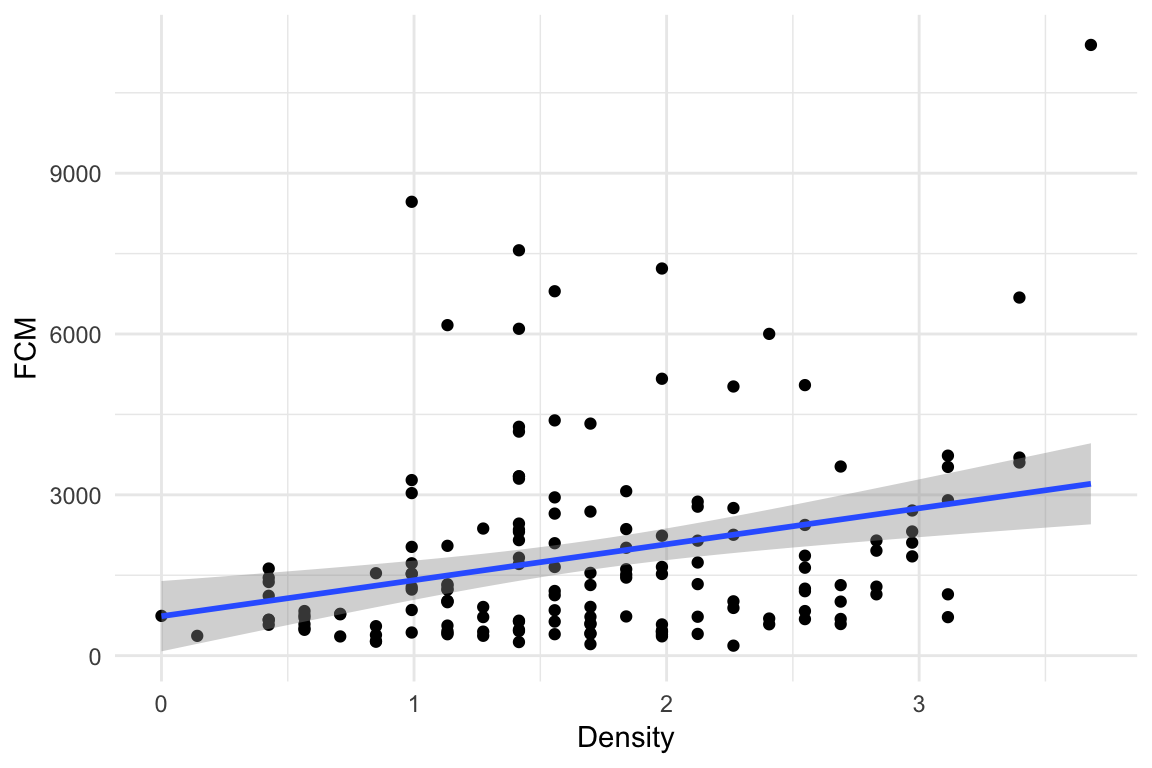
\includegraphics{Walker-elementary-statistical-modeling-draft_files/figure-latex/squirrel-1.pdf}
\caption{\label{fig:squirrel}A scatterplot of Fecal cortisol matabolites and
squirrel density.}
\end{figure}

Figure \ref{fig:squirrel} is a \textbf{scatterplot} of the data with the
amount of cortisol metabolites in the feces on the \(Y\) axis and local
squirrel density on the \(X\) axis. The line through the data is a
graphical representation of a linear model fit to the data and the gray
cloud around the line is a graphical representation of the uncertainty
in the model. The researchers wanted to model the ``effect'' of squirrel
density on the amount of cortisol metabolites in the feces of the
pregnant mothers. Graphically, this effect is the slope of the line in
Figure \ref{fig:squirrel}.

The model fit to the data is

\begin{equation}
FCM_i = \beta_0 + \beta_1 Density_i + \varepsilon_i
\label{eq:fcm-model}
\end{equation}

which contains both the linear predictor and the error. For inference,
for example, computing standard errors of the coefficients, We need to
model the error. Here, we use the simplest model of error which is ``IID
\(N(0, \sigma)\)''. This means, the modeled error is

\begin{enumerate}
\def\labelenumi{\arabic{enumi}.}
\tightlist
\item
  Independent -- individual error values are independent of other
  values.
\item
  Identical -- individual error can be thought of as a sample from a
  single \textbf{random distribution} (the same for each individual
  value). For this model, this distribution is
\item
  \(N(0, \sigma)\) -- the modeled distribution is ``Normal'' or
  ``Gaussian'', with a mean of zero and a standard deviation of
  \(\sigma\).
\end{enumerate}

The predictor part of the model is

\begin{equation}
\textrm{E}[FCM|Density] = \beta_0 + \beta_1 Density
\label{eq:regression}
\end{equation}

In words, model \eqref{eq:regression} reads ``the expected value of
\(FCM\) conditional on density is beta-knot plus beta-one times
density''. An \textbf{expected value} is a long run average -- if we
were to sample lots and lots of red squirrel populations with
\(Density=x\) (where \(x\) is a specific value), we'd expect the average
\(FCM\) across these samples to be \(\beta_0 + \beta_1 x\).

\begin{quote}
Let's unpack this. \(\textrm{E}[Y]\) is the \textbf{expectation} or
\textbf{expected value} of \(Y\). An expection is the long-run average
of \(Y\) if we were to run an experiment or re-sample a population many
times. The sample mean of \(Y\) is an estimate of \(\textrm{E}[Y]\).
\(\textrm{E}[Y|X]\) is a conditional expectation of \(Y\) -- it is the
expectation given additional conditions. Using the red squirrel example,
these conditions are a specific value of \(Density\). If \(FCM\) is
linearly related to \(Density\) (the right-hand side of equation
\eqref{eq:regression}) then the expected value of \(FCM\) given a local
density of 2.8 squirrels differs from the expected value of \(FCM\)
given a local density of 1.4 squirrels (the units of \(Density\) are
squirrels per 150 meter radius of the individual female's midden).
\end{quote}

In model \eqref{eq:regression}, there is a single \(X\) variable
(\(FCM\)). While the \(X\) variables are often called the ``dependent''
variables, in this model \(FCM\) does not ``depend'' on the independent
variable \(Density\) in any causal sense -- meaning if I were to
intervene and set \(Density\) to some value \(x\), I would expect
\(FCM\) to equal \(\beta_0 + \beta_1 x\). Rather, \(FCM\) only
``depends'' on \(Density\) in a probablistic sense -- if \(Density = x\)
then the most probable value of \(FCM\) is \(\beta_0 + \beta_1 x\). With
some strong assumptions model \eqref{eq:regression} can be turned into a
model of causal dependency, which is the focus of chapter xxx.

\(\beta_0\) and \(\beta_1\) are the \textbf{parameters} of model
\eqref{eq:regression}. Specifically \(\beta_0\) is the model
\textbf{intercept} and \(\beta_1\) is the modeled \textbf{effect} of
\(Density\). Again, the effect (\(\beta_1\)) has a probabilistic, and
not causal, interpretation. This interpretation is

\begin{equation}
\beta_1 = \textrm{E}[FCM|Density=x+1] - \textrm{E}[FCM|Density=x] 
\label{eq:beta1}
\end{equation}

Or, in words, ``beta-1 is the expected value of FCM when density equals
x + 1 minus the expected value of FCM when the density equals x.''
\(\beta_1\) is simply the difference in expected values given a one unit
difference in \(Density\). A very short way to state this is
``\(\beta_1\) is a difference in conditional means''.

\subsection{Using a linear model to estimate explanatory
effects}\label{using-a-linear-model-to-estimate-explanatory-effects}

The goal of the statistical model here is to estimate \(\beta_1\) -- the
probabalistic effect of \(Density\) on \(FCM\). This estimate, and a
measure of the uncertainty of this estimate, are in the table of
coefficients of the fit model

\begin{tabular}{l|r|r|r|r}
\hline
  & Estimate & Std. Error & t value & Pr(>|t|)\\
\hline
(Intercept) & 736.0 & 331.9 & 2.2 & 0.0281\\
\hline
Density & 671.1 & 178.9 & 3.8 & 0.0002\\
\hline
\end{tabular}

where the entries in the column ``Estimate'' are estimates of the
parameters \(\beta_0\) and \(\beta_1\) in model \eqref{eq:regression}. The
entries in the column ``Std. Error'' are the standard errors (SE) of the
estimates, which are measures of the uncertainty of the estimates.

The parameter estimates in the table above are the coefficients of the
fitted model

\begin{equation}
FCM_i = b_0 + b_1 Density_i + e_i
\label{eq:fcmi}
\end{equation}

where the subscript \emph{i} refers to the \emph{i}th individual. The
coefficients \(b_0\) and \(b_1\) are the y-intercept and the slope of
the line in Figure \ref{fig:squirrel}. The coefficient for \(Density\)
(\(b_1\)) is 671.1, and (given the definition of the parameter
\(\beta_1\) in equation \eqref{eq:beta1}) we expect squirrel mothers with
a local density of 2 squirrels within a 150 m radius of her midden to
average 671.1 more units of FCM (ng of fecal cortical metabolites per
gram dry food) than mother squirrels with a local density of only 1
squirrel within a 150 m radius of her midden.

\subsubsection{Probabilistic vs.~causal
conditioning}\label{probabilistic-vs.causal-conditioning}

Remember that this coefficient is estimating a probabilistic parameter.
Consequently, the coefficient \(b_1\) is simply a descriptor of a
pattern of relationship between local density and fecal cortisol
metabolites - no causal effect is implied. With the strong assumptions
explained in chapter xxx, however, \(b_1\) can estimate a causal effect.

\subsection{Using a linear model for
prediction}\label{using-a-linear-model-for-prediction}

Model \eqref{eq:fcmi} gives the measured value of \emph{FCM} for each
squirrel. The equation includes the linear predictor
(\(b_0 + b_1 Density_i\)) and the \textbf{residual} from the predictor
(\(e_i\)). The predictor part is called ``predictor'' because it is the
equation for predicting the value of an individual's \(FCM\) given that
individual's value of \(Density\):

\begin{equation}
\widehat{FCM} = b_0 + b_1 Density
\label{eq:fcmhat}
\end{equation}

where \(\widehat{FCM}\) is read as ``FCM hat'' and is the
\textbf{predicted value} or simply ``prediction''. Very often, we use
the predictor part (equation \eqref{eq:fcmhat}) to predict unknown or
future values given different modeled inputs (the \(X\)).

\subsection{Reporting results}\label{reporting-results}

The authors of the squirrel fcm data published a figure and table
similar to fig. xxx and table above but used a slightly more complex
linear model. Here is how the author's reported the results:

\begin{quote}
Across 6 years (2006 to 2011), we found a positive relationship between
local density and concentrations of fecal cortisol metabolites {[}FCM;
t\(_155\) = 3.63, P = 0.0002 (table S4 and Fig. 3A){]}.
\end{quote}

I would advocate reporting the estimate and a confidence interval
instead of \(t\) and \(p\). For example ``Across 6 years (2006 to 2011),
the probabilistic effect of local density on fecal cortisol metabolites
is 671.1 (95\% CI: 317.7, 1024.5). If a \(p\)-value is report \emph{in
addition} to the effect and CI, always report the exact \emph{p}-value,
which emphasizes the continuous nature of evidence against the null, and
not something like''\(p < 0.05\)``, which artificially dichotomizes the
evidence against the null.

\section{Working in R}\label{working-in-r}

\subsection{\texorpdfstring{Exploring the bivariate relationship between
\emph{Y} and
\emph{X}}{Exploring the bivariate relationship between Y and X}}\label{exploring-the-bivariate-relationship-between-y-and-x}

Questions

\begin{enumerate}
\def\labelenumi{\arabic{enumi}.}
\tightlist
\item
  Import the ``FCM data dryad.csv'' data from the Dryad repository as
  the data.table \texttt{fcm}
\item
  How are different words in the column labels demarcated? Is this good
  practice?
\end{enumerate}

Here we want to fit a model of \texttt{FCM.ng.g.dry} as a function of
\texttt{Raw.Squirrel.Density}. The authors used prior knowledge to
expect a positive relationship between these two variables. Use qplot to
generate a scatterplot of \(FCM\) against \(Density\)

Questions

\begin{enumerate}
\def\labelenumi{\arabic{enumi}.}
\setcounter{enumi}{2}
\tightlist
\item
  Is there a trend? If so, does the trend look linear or non-linear?
\item
  Does the residual variation (the deviation from the trend on the \(Y\)
  axis) look homogenous along the \(X\)-axis?
\item
  Are there any obvious outliers?
\end{enumerate}

\subsection{Fitting the linear model}\label{fitting-the-linear-model}

We will fit a linear model to the data using the \texttt{lm} function,
which is very general and will be our workhorse throughout the class.
The minimal input to the function is a model formula and the name of the
data.frame (remember, a data.table is a data.frame). A formula is of the
form \texttt{Y\ \textasciitilde{}\ X}. All of the output we assign to
the object \texttt{fit}.

Let's fit the linear model to the data using density as the predictor

\begin{Shaded}
\begin{Highlighting}[]
\NormalTok{  fit <-}\StringTok{ }\KeywordTok{lm}\NormalTok{(FCM.ng.g.dry }\OperatorTok{~}\StringTok{ }\NormalTok{Raw.Squirrel.Density, }\DataTypeTok{data=}\NormalTok{fcm)}
\end{Highlighting}
\end{Shaded}

R will look for the specified \(Y\) and \(X\) variables in the column
names of \texttt{fcm}. If these are not found, R will return an error,
for example

\begin{Shaded}
\begin{Highlighting}[]
\NormalTok{  fit <-}\StringTok{ }\KeywordTok{lm}\NormalTok{(FCM_ng_g_dry }\OperatorTok{~}\StringTok{ }\NormalTok{Raw_Squirrel_Density, }\DataTypeTok{data=}\NormalTok{fcm)}
\end{Highlighting}
\end{Shaded}

will return the error ``Error in eval(predvars, data, env) : object
`FCM\_ng\_g\_dry' not found''. This means your spelling and
capitalization have to be exact!

\subsection{\texorpdfstring{Getting to know the linear model: the
\texttt{summary}
function}{Getting to know the linear model: the summary function}}\label{getting-to-know-the-linear-model-the-summary-function}

The \texttt{lm} function returns an \texttt{lm} object, which we've
assigned to the name \texttt{fit}. \texttt{fit} contains lots of
information about our fit of the linear model to the data. Most of the
information that we want for most purposes can be retrieved with the
\texttt{summary} function, which is a general-purpose R command the
works with many R objects.

\begin{Shaded}
\begin{Highlighting}[]
\KeywordTok{summary}\NormalTok{(fit)}
\end{Highlighting}
\end{Shaded}

\begin{verbatim}
## 
## Call:
## lm(formula = FCM.ng.g.dry ~ Raw.Squirrel.Density, data = fcm)
## 
## Residuals:
##     Min      1Q  Median      3Q     Max 
## -2107.5 -1108.3  -434.9   511.8  8186.8 
## 
## Coefficients:
##                      Estimate Std. Error t value Pr(>|t|)    
## (Intercept)             736.0      331.9   2.217 0.028078 *  
## Raw.Squirrel.Density    671.1      178.9   3.752 0.000248 ***
## ---
## Signif. codes:  0 '***' 0.001 '**' 0.01 '*' 0.05 '.' 0.1 ' ' 1
## 
## Residual standard error: 1732 on 154 degrees of freedom
##   (7 observations deleted due to missingness)
## Multiple R-squared:  0.08374,    Adjusted R-squared:  0.07779 
## F-statistic: 14.07 on 1 and 154 DF,  p-value: 0.0002484
\end{verbatim}

What is here:

\textbf{Call}. This is the model that was fit

\textbf{Residuals}. This is a summary of the distribution of the
residuals. From this one can get a sense of the distribution (for
inference, the model assumes a normal distribution with mean zero). More
useful ways to examine this distribution will be introduced later in
this chapter.

\textbf{Coefficients table}. This contains the linear model coefficients
and their standard error and associated \(t\) and \(p\) values.

\begin{enumerate}
\def\labelenumi{\arabic{enumi}.}
\tightlist
\item
  The column of values under ``Estimate'' are the coefficients of the
  fitted model (equation \eqref{eq:fcmi}). Here, 735.9604344 is the
  intercept (\(b_0\)) and 671.1379749 is the effect of \(Density\)
  (\(b_1\)).
\item
  The column of values under ``Std. Error'' are the standard errors of
  the coefficients.
\item
  The column of values under ``t value'' are the \emph{t-statistics} for
  each coefficient. A \(t\)-value is a \textbf{signal to noise ratio}.
  The coefficient \(b_1\) is the ``signal'' and the SE is the noise. Get
  used to thinking about this ratio. Any \(t\) less than 2 is indicative
  of too much noise to say much about the signal. A \(t\) between 2 and
  3 means the noise is large enough to suggest an effect. A \(t\)
  greater than 3 is pretty good evidence of an effect.
\item
  The column of values under ``Pr(\textgreater{}\textbar{}t\textbar{})''
  is the \(p\)-value, which is the exact probability associated with a
  particular \(t\). What is the \(p\)-value a test of? The \(p\)-value
  tests the hypothesis ``how probable are the data if the coefficient is
  zero?''. Formally \(P = \mathrm{freq(t' \ge t|H_o)}\), where \(t'\) is
  the hypothetical t-value, t is the observed \(t\)-value, and \(H_o\)
  is the null hypothesis. We will return to \(p\)-values in Chapter xxx.
\end{enumerate}

\textbf{Signif. codes}. I am surprised that base R returns this. These
are useless because the concept of ``levels of significance'' is
muddled, as will be discussed in Chapter xxx.

Beneath the Signif. codes are some model statistics which are useful

\textbf{Residual standard error} This is \(\sqrt{\sum{e_i^2}/(n-2)}\),
where \(e_i\) are the residuals in the fitted model. ``degrees of
freedom'' is the number of \(e_i\) that are ``allowed to vary'' after
fitting the parameters, so is the total sample size (\(n\)) minus the
number of parameters fit. The fit model has two fit parameters (\(b_0\)
and \(b_1\) so the df is \(n-2\). Note that this is the denominator in
the residual standard error equation.

\textbf{Multiple R-squared}. This is an important but imperfect summary
measure of the whole model that effectively measures how much of the
total variance in the response variable ``is explained by'' the model.
Its value lies between zero and 1. \textbf{It's a good measure to report
in a manuscript}.

\textbf{F-statistic and p-value}. These are statistics for the whole
model (not the individual coefficients) and I just don't find these very
useful.

Note that the \(p\)-value for the coefficient for Raw.Squirrel.Density
is very small and we could conclude that the data are not consistant
with a model of no slope. But did we need a formal hypothesis test for
this? We haven't learned much if we have only learned that the slope is
``not likely to be exactly zero''. What we want to know is not \emph{if}
there is a relationship between \(FCM\) and \(Density\), which is
imperfectly answered with a \(p\)-value, but \emph{the sign and
magnitude} of the relationship and the uncertainty in this estimate. For
this, we don't need the \(p\)-value. Instead, we want to interpret the
coefficient to its SE directly (for a quick-and-dirty interpretation) or
the confidence interval of the effect (for a more formal
interpretation). Please read this paragraph again. We will come back to
it over and over.

\subsection{display: An alternative to
summary}\label{display-an-alternative-to-summary}

Much of what we want to know about a model fit is returned by the
\texttt{display} function from the \texttt{arm} package.

\begin{Shaded}
\begin{Highlighting}[]
\KeywordTok{display}\NormalTok{(fit)}
\end{Highlighting}
\end{Shaded}

\begin{verbatim}
## lm(formula = FCM.ng.g.dry ~ Raw.Squirrel.Density, data = fcm)
##                      coef.est coef.se
## (Intercept)          735.96   331.94 
## Raw.Squirrel.Density 671.14   178.90 
## ---
## n = 156, k = 2
## residual sd = 1732.02, R-Squared = 0.08
\end{verbatim}

The \texttt{display} function does not give a \(t\)-value or a
\(p\)-value of the coefficients because the authors of the arm package
do not think \(p\)-values are very valuable. We don't need a \(t\)
because one can mentally compute the approximate ratio of the
coefficient to its SE and get a sense of the signal to noise, and that's
all the authors of the display function think we need.

\subsection{Confidence intervals}\label{confidence-intervals}

Confidence intervals for the coefficients of the model are obtained by

\begin{Shaded}
\begin{Highlighting}[]
\KeywordTok{confint}\NormalTok{(fit)}
\end{Highlighting}
\end{Shaded}

\begin{verbatim}
##                          2.5 %   97.5 %
## (Intercept)           80.21785 1391.703
## Raw.Squirrel.Density 317.73057 1024.545
\end{verbatim}

\texttt{confint} returns by default the 95\% confidence interval (CI) of
all parameters. The most useful way of thinking about the meaning of a
CI is

\textbf{A confidence interval contains the range of parameter values
that are consistent with the data, in the sense that a \(t\)-test would
not reject the null hypothesis of a difference between the estimate and
any value within the interval}

A more textbook way of defining a CI is: A 95\% CI of a parameter has a
95\% probability of including the true value of the parameter. It does
not mean that there is a 95\% probability that the true value lies in
the interval. This is a subtle but important difference. Here is a way
of thinking about the proper meaning of the textbook definition: we
don't know the true value of \(\beta_1\) but we can 1) repeat the
experiment or sampling, 2) re-estimate \(\beta_1\), and 3) re-compute a
95\% CI. If we do 1-3 many times, 95\% of the CIs will include
\(\beta_1\) within the interval.

Confidence intervals are often interpreted like \(p\)-values. That is,
the researcher looks to see if the CI overlaps with zero and if it does,
concludes there is ``no effect''. First, this conclusion is not correct
-- \textbf{the inability to find sufficient evidence for an effect does
not mean there is no effect, it simply means there is insufficient
evidence to conclude there is an effect}!

Second, what we want to use the CI for is to guide us about how big or
small the effect might reasonably be, given the data. Again, A CI is a
measure of parameter values that are ``consistent'' with the data. If
our biological interpretations at the small-end and at the big-end of
the interval's range radically differ, then we don't have enough
\emph{precision} in our analysis to reach an unambiguous conclusion.
Remember this.

\subsection{How good is our model?}\label{how-good-is-our-model}

How well does variation in \(Density\) ``explain'' variation in \(FCM\)?
The answer to this is in the \(R^2\) value, which is given in
\texttt{display(fit)} and in \texttt{summary(fit)} and accessed directly
with

\begin{Shaded}
\begin{Highlighting}[]
\KeywordTok{summary}\NormalTok{(fit)}\OperatorTok{$}\NormalTok{r.squared}
\end{Highlighting}
\end{Shaded}

\begin{verbatim}
## [1] 0.08373756
\end{verbatim}

\(R^2\) is the fraction of the total variance of \(Y\) explained by the
model, or more specifically, the linear predictor. It will vary from
zero (the model explains nothing) to one (the model explains
everything). If \(R^2=0\) the response is completely unpredictable by
the predictors. We can think of the values of the response as white
noise or all error. This doesn't mean that the values are ``not caused''
or ``random'' or not predicted by some other variable. It only means the
values are random with respect to the \(X\) variable(s) in the model. If
\(R^2=1\) we can \emph{exactly} predict the response from the \(X\)
variables in the model. So the bigger the \(R^2\), the better the model
in the sense that the response is more predicatable. \textbf{Super
importantly}, ``explains'' is in a probabilistic and not causal sense.
We will explore this concept much more in future worksheets.

\subsection{Model checking}

\texttt{plot} is a very useful base R function for ``model checking'' or
``model diagnostics'' to see if our model fit is acceptable.

\begin{Shaded}
\begin{Highlighting}[]
\KeywordTok{plot}\NormalTok{(fit)}
\end{Highlighting}
\end{Shaded}

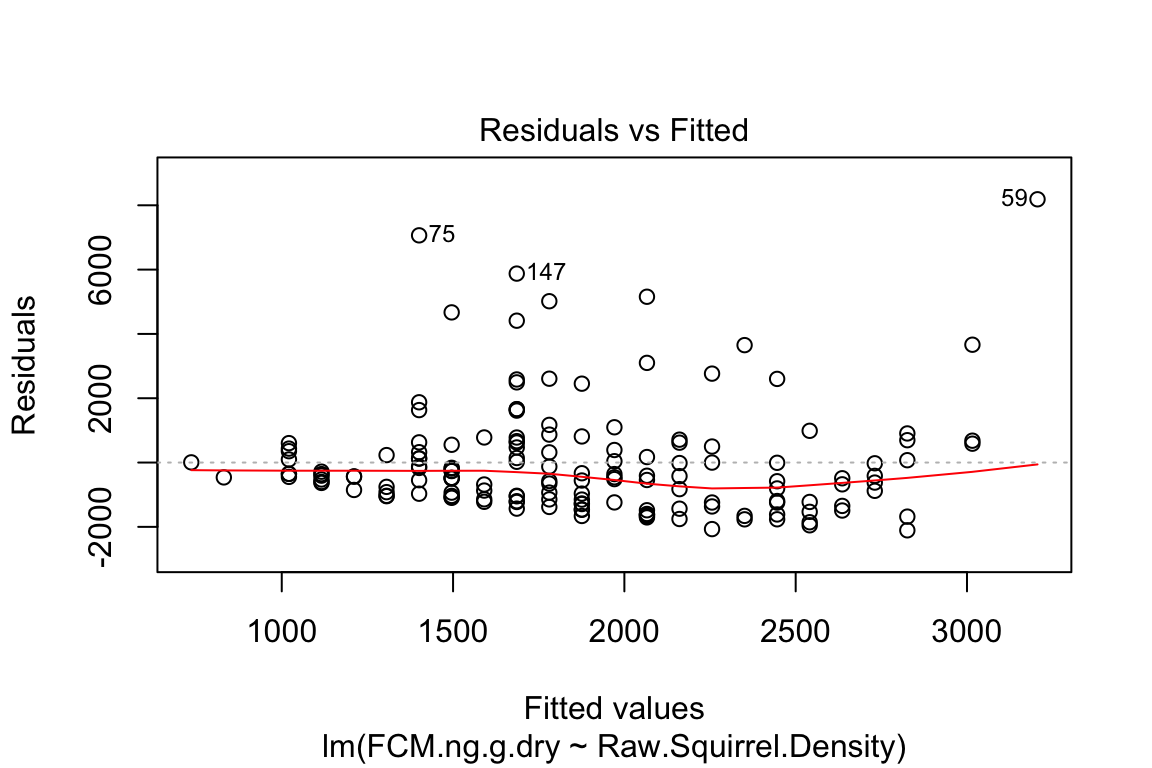
\includegraphics{Walker-elementary-statistical-modeling-draft_files/figure-latex/fit-diagnostics-1.pdf}
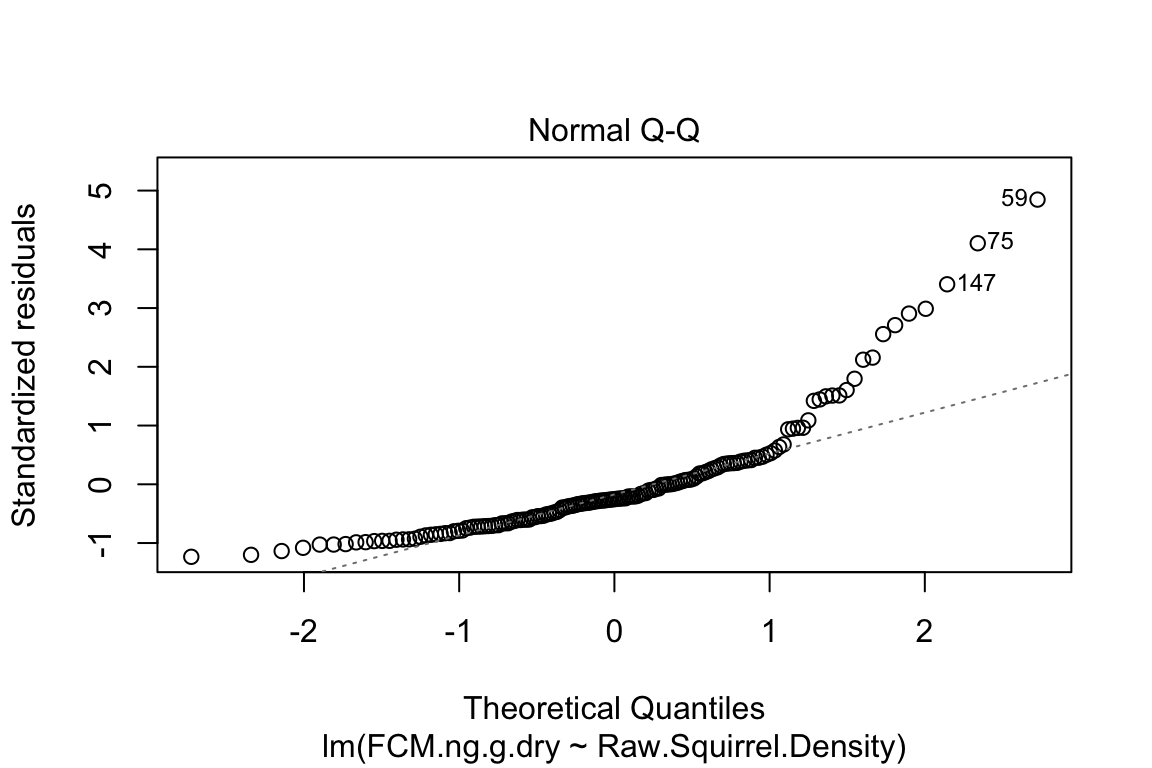
\includegraphics{Walker-elementary-statistical-modeling-draft_files/figure-latex/fit-diagnostics-2.pdf}
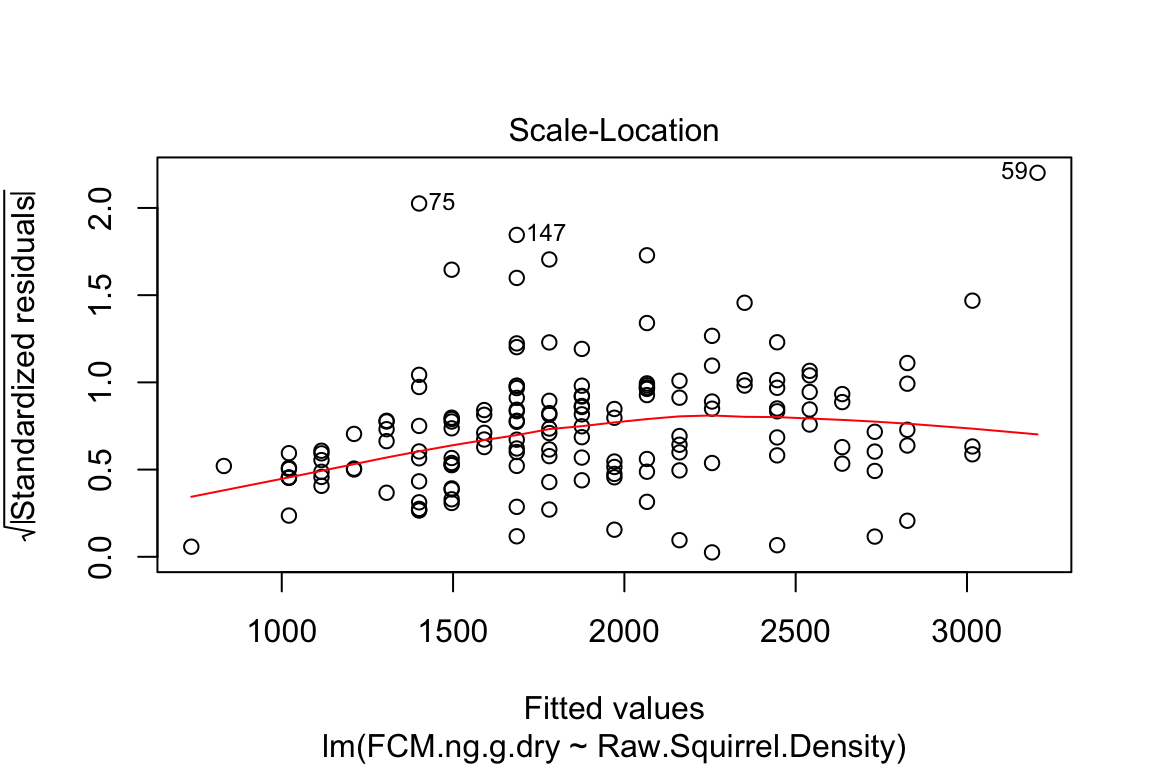
\includegraphics{Walker-elementary-statistical-modeling-draft_files/figure-latex/fit-diagnostics-3.pdf}
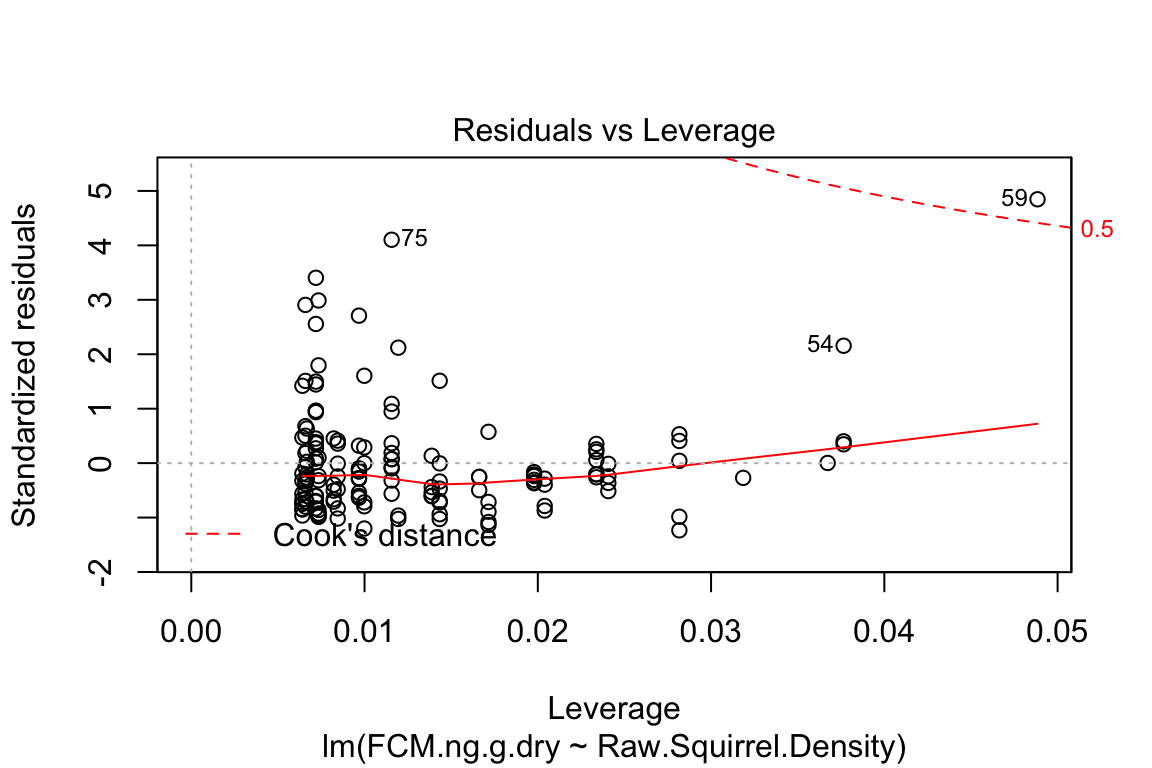
\includegraphics{Walker-elementary-statistical-modeling-draft_files/figure-latex/fit-diagnostics-4.pdf}

Compare the four diagnostic plots using the guidelines from here
\url{http://data.library.virginia.edu/diagnostic-plots/}

Questions

\begin{enumerate}
\def\labelenumi{\arabic{enumi}.}
\setcounter{enumi}{5}
\tightlist
\item
  Look at the plots you just made. What is a residual? What is a fitted
  value?
\end{enumerate}

\subsection{exploring a lm object}\label{exploring-a-lm-object}

\texttt{fit} contains much information but simply typing \texttt{fit}
into the console gives us only the model and the coefficients.
\texttt{names} is a super important R function. It gives us the names of
all the parts of some R object. \texttt{fit} is an lm object.
\texttt{names(fit)} gives us all the parts contained in an lm object.

\begin{Shaded}
\begin{Highlighting}[]
\KeywordTok{names}\NormalTok{(fit)}
\end{Highlighting}
\end{Shaded}

\begin{verbatim}
##  [1] "coefficients"  "residuals"     "effects"       "rank"         
##  [5] "fitted.values" "assign"        "qr"            "df.residual"  
##  [9] "na.action"     "xlevels"       "call"          "terms"        
## [13] "model"
\end{verbatim}

You can see any of these parts using the dollar sign

Questions

\begin{enumerate}
\def\labelenumi{\arabic{enumi}.}
\setcounter{enumi}{6}
\item
  What does \texttt{fit\$residuals} return? Answer using equation
  \eqref{eq:fcmi}
\item
  What does \texttt{fit\$fitted.values} return? Answer using equation
  @ref(eq:fcmi
\end{enumerate}

You can use qplot to make a plot similar to the first plot of
\texttt{plot(fit)}

\begin{Shaded}
\begin{Highlighting}[]
\KeywordTok{qplot}\NormalTok{(fit}\OperatorTok{$}\NormalTok{fitted.values, fit}\OperatorTok{$}\NormalTok{residuals, }\DataTypeTok{geom=}\KeywordTok{c}\NormalTok{(}\StringTok{'point'}\NormalTok{, }\StringTok{'smooth'}\NormalTok{))}
\end{Highlighting}
\end{Shaded}

\begin{verbatim}
## `geom_smooth()` using method = 'loess' and formula 'y ~ x'
\end{verbatim}

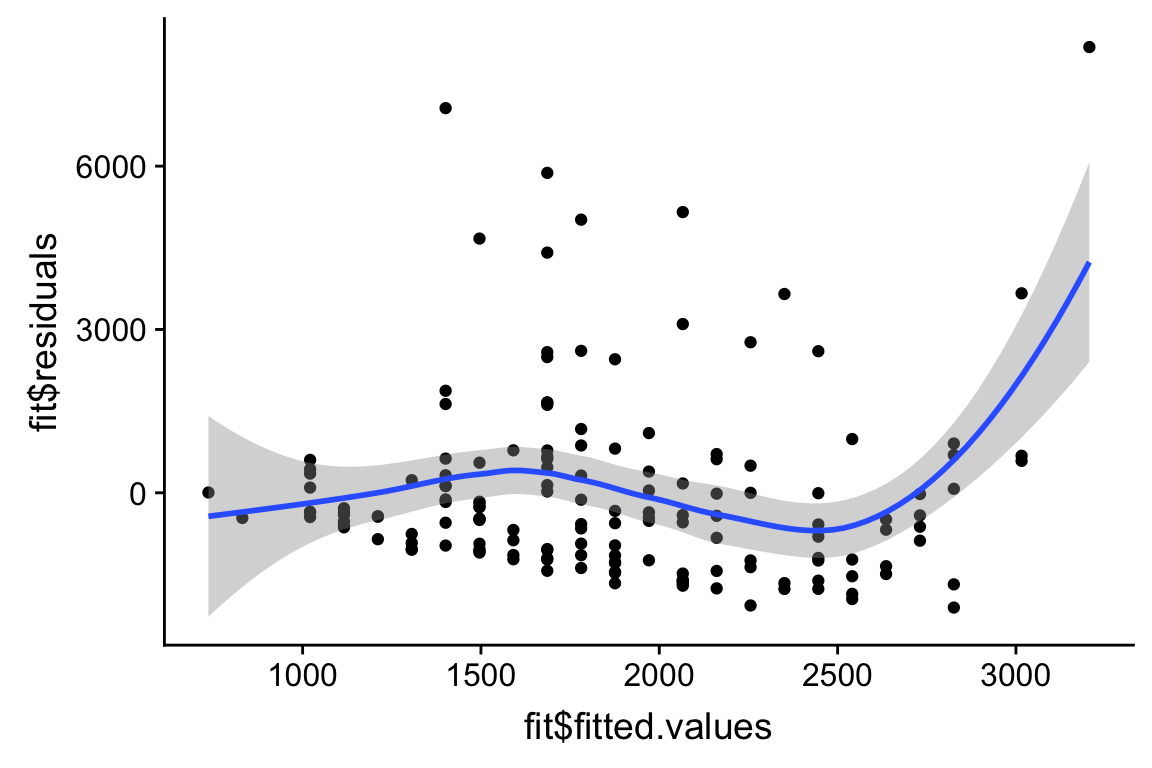
\includegraphics{Walker-elementary-statistical-modeling-draft_files/figure-latex/fit-fitted-1.pdf}

\section{Problems}\label{problems-2}

\begin{enumerate}
\def\labelenumi{\arabic{enumi}.}
\tightlist
\item
  Using the chick data from Chapter 3. Compare the effects of
  nest\_temperature\_above\_ambient on day13\_mass by fitting two
  separate linear models 1) one using only the control group and one
  using the treated group. The grouping variable is playback\_treatment.
  These models were plotted in Chapter 3 so \texttt{lm} will return the
  linear model behind these plots.
\end{enumerate}

Report the results using the two effect estimates and a 95\% confidence
interval (we will learn in a later chapter a more sophisticated way of
comparing the effects between the groups)

\textbf{file name}: ``allDatasetsMarietteBuchanan2016.xls''

\textbf{source}: \url{https://datadryad.org//handle/10255/dryad.122315}

\begin{enumerate}
\def\labelenumi{\arabic{enumi}.}
\setcounter{enumi}{1}
\tightlist
\item
  (Grad students only) -- find a dataset using Dryad that has data that
  can be fit by a simple linear model with a single continuous \(X\)
  (its okay if the authors fit the data with a more complex model). Fit
  the data and report the results with a plot and text.
\end{enumerate}

\chapter{\texorpdfstring{A linear model with a single, categorical
\emph{X}}{A linear model with a single, categorical X}}\label{a-linear-model-with-a-single-categorical-x}

\section{\texorpdfstring{A linear model with a single, categorical
\emph{X} is the engine behind a single factor (one-way) ANOVA and a
t-test is a special case of this
model.}{A linear model with a single, categorical X is the engine behind a single factor (one-way) ANOVA and a t-test is a special case of this model.}}\label{a-linear-model-with-a-single-categorical-x-is-the-engine-behind-a-single-factor-one-way-anova-and-a-t-test-is-a-special-case-of-this-model.}

To introduce modeling with a single, categorical \(X\) variable, I'll
use the vole data from

\begin{enumerate}
\def\labelenumi{\arabic{enumi}.}
\tightlist
\item
  Source: Dryad Digital Repository.
  \url{https://doi.org/10.5061/dryad.31cc4/1}
\item
  File: ``RSBL-2013-0432 vole data.xlsx''
\item
  Sheet: ``COLD VOLES LIFESPAN''
\end{enumerate}

Normal cellular metabolism creates reactive oxygen species (ROS) that
can disrupt cell function and potentially cause cell damage.
Anti-oxidants are molecules that bind ROS, inhibiting their ability to
disrupt cell activity. A working hypothesis for many years is that
supplemental anti-oxidants should improve cell function and, scaling up,
whole-animal function (such as lifespan). The vole data explores this
with supplemental Vitamins C and E, which are anti-oxidants, in the diet
of the short-tailed field vole (\emph{Microtus agrestis}).

The goal of the study is to measure the effect of anti-oxidants on
lifespan. The researchers randomly assigned the voles to one of thre
treatment levels: ``control'', ``vitamin E'', and ``vitamin C''. The
variable \(treatment\), is a single, categorical \(X\) variable.
Categorical variables are often called \textbf{factors} and the
treatment levels are often called \textbf{factor levels}. There are no
units to a categorical \(X\) variable (even though a certain amount of
each anti-oxidant was supplemented). The response (\(Y\)) is
\(lifespan\) measured in days.

The linear model with a categorical \(X\) variable with three levels is
not immediately obvious, and so I don't present the model until after
showing the table of model coefficients

\subsection{Table of model
coefficients}\label{table-of-model-coefficients}

Here is the table of coefficients from the linear model fit

\begin{tabular}{l|r|r|r|r}
\hline
  & Estimate & Std. Error & t value & Pr(>|t|)\\
\hline
(Intercept) & 503.4 & 27.4 & 18.4 & 0.000\\
\hline
treatmentvitamin\_E & -89.9 & 52.5 & -1.7 & 0.090\\
\hline
treatmentvitamin\_C & -115.1 & 54.5 & -2.1 & 0.037\\
\hline
\end{tabular}

The table has estimates for three parameters. The first estimate (the
intercept) is the mean response in the reference level. Here the
reference level is the ``control'' group. The additional estimates are
the differences in the mean between each of the other treatment levels
and the reference level. These are the ``effects'' in the model. So
typically with categorical \(X\), when we speak of an \emph{effect} we
mean a difference in means. These estimates and their meaning are
illustrated in Figure \ref{fig:vole-mean-plot}.

(note. The default in R is to set the level that is first alphabetically
as the reference level. In the vole data, ``control'' comes before
``vitamin\_E'' and ``vitamin\_C'' alphabetically, and so by default, it
is the reference level. This makes sense for these data -- we want to
compare the lifespan of the vitamins E and C groups to that of the
control group. The reference level can be changed of course.)

\begin{figure}
\centering
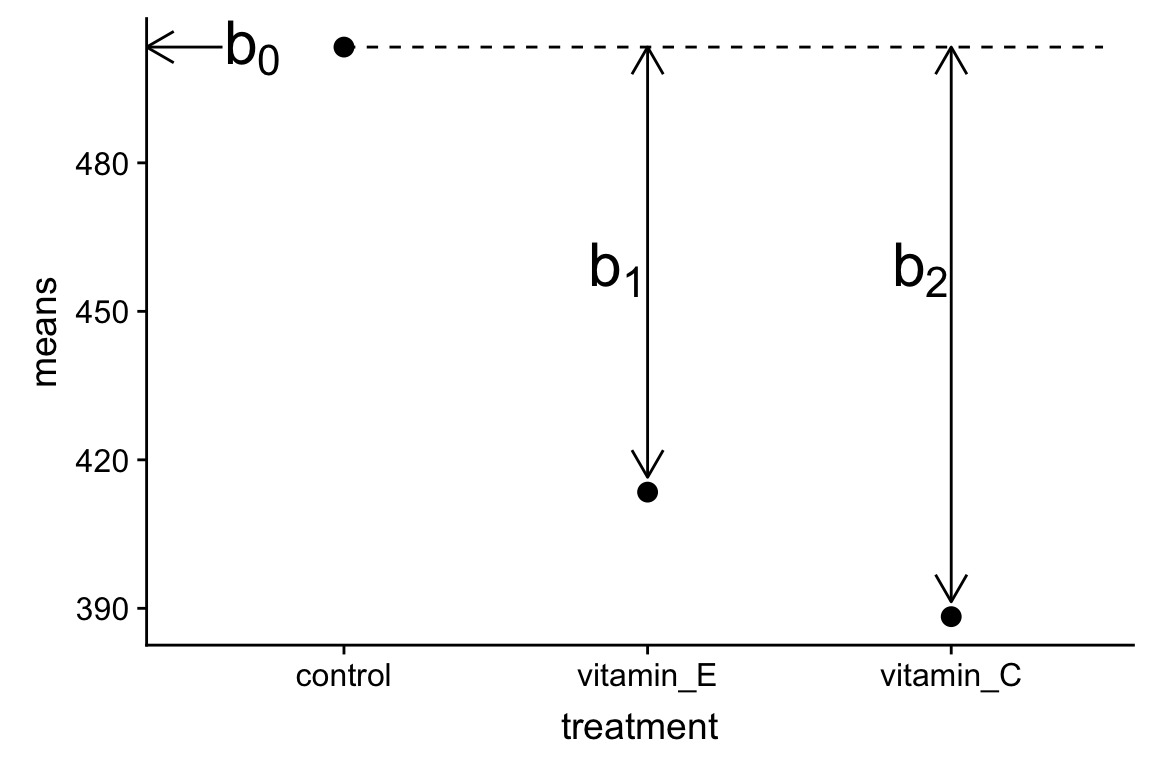
\includegraphics{Walker-elementary-statistical-modeling-draft_files/figure-latex/vole-mean-plot-1.pdf}
\caption{\label{fig:vole-mean-plot}What the coefficients of a linear model
with a single categorical X mean. The means of the three treatment
levels for the vole data are shown with the filled circles. The length
of the double-headed arrows are differences in means. The intercept
(\(b_0\)) is the mean of the reference treatment level. The coefficients
(\(b_1\) and \(b_2\)) are the differences between the treatment level's
mean and the reference mean. As with a linear model with a continuous X,
the coefficients are effects.}
\end{figure}

\subsection{The linear model}\label{the-linear-model}

We can see an immediate difference between the coefficient table for a
linear model fit to a single, categorical \(X\) and that for a single,
continuous \(X\). For the latter, there is a single coefficient for
\(X\). For the former, there is a coefficient for each level of the
categorical \(X\) \emph{except} the ``reference'' level.

The linear model for a single, continuous \(X\) with three factor levels
is

\begin{equation}
lifespan = \beta_0 + \beta_1 vitamin\_E + \beta_2 vitamin\_C + \varepsilon
\end{equation}

and the estimates in the coefficient table are the coefficients of the
fit model

\begin{equation}
lifespan_i = b_0 + b_1 vitamin\_E + b_2 vitamin\_C + e_i
\label{eq:model-cat-x}
\end{equation}

Remember, \(b_0\) is the mean of the control group, \(b_1\) is the
difference in means between the vitamin E and control groups, and
\(b_2\) is the difference in means between the vitamin C and control
groups (Figure \ref{fig:vole-mean-plot}).

In this model, \(vitamin\_E\) and \(vitamin\_C\) are \textbf{dummy
variables} that contain a one, if the data is from that treatment level,
and zero otherwise. This is called dummy coding or treatment coding. The
\texttt{lm} function creates these dummy variables under the table, in
something called the \textbf{model matrix}, which we'll cover in the
next chapter. You won't see these columns in your data. But if you did,
it would look something like this

\begin{tabular}{r|l|r|r}
\hline
lifespan & treatment & vitamin\_E & vitamin\_C\\
\hline
621 & control & 0 & 0\\
\hline
865 & control & 0 & 0\\
\hline
583 & vitamin\_E & 1 & 0\\
\hline
561 & vitamin\_E & 1 & 0\\
\hline
315 & vitamin\_C & 0 & 1\\
\hline
157 & vitamin\_C & 0 & 1\\
\hline
\end{tabular}

There are alternative coding methods. Dummy coding is the default in R.
Note that the method of coding can make a difference in an ANOVA table,
and many published papers using R have published incorrect
interpretations of ANOVA table outputs. This is both getting ahead of
ourselves and somewhat moot, because I don't advocate publishing ANOVA
tables.

\subsubsection{\texorpdfstring{Some math to convince you that the
intercept of a linear model with a categorical \(X\) is the mean of the
reference group \emph{and} the intercept of a line. And some math to
convince you that the coefficient of a dummy variable in a linear model
with a categorial \(X\) is a difference in means \emph{and} a
slope.}{Some math to convince you that the intercept of a linear model with a categorical X is the mean of the reference group and the intercept of a line. And some math to convince you that the coefficient of a dummy variable in a linear model with a categorial X is a difference in means and a slope.}}\label{some-math-to-convince-you-that-the-intercept-of-a-linear-model-with-a-categorical-x-is-the-mean-of-the-reference-group-and-the-intercept-of-a-line.-and-some-math-to-convince-you-that-the-coefficient-of-a-dummy-variable-in-a-linear-model-with-a-categorial-x-is-a-difference-in-means-and-a-slope.}

The interecept of a model is the value of the model when all
\(X\)-variables are set to zero. The \(X\) variables in the model
(Equation \eqref{eq:model-cat-x}) are the dummy variables \(vitamin\_E\)
and \(vitamin\_C\). If we set vitamin\_E\$ and \(vitamin\_C\) in
Equation \eqref{eq:model-cat-x} to zero, the modeled (or expected) value
reduces to

\begin{equation}
\mathrm{E}(lifespan|X_1=0, X_2=0) = b_0
\end{equation}

\% Since both dummy variables are set to zero, we have modeled the
expected value or mean of the control group.

The slope of a model is the difference in the modeled value given a one
unit increase in \(X\). If we increase the dummy variable \(vitamin\_E\)
from zero to one (that is, if we are modeling the expected value of the
vitamin E group), we get

\begin{equation}
\mathrm{E}(lifespan|X_1=1, X_2=0) = b_0 + b_1
\end{equation}

which can be re-arranged to

\begin{equation}
b_1 = \mathrm{E}(lifespan|X_1=1, X_2=0) - b_0
\end{equation}

and since \(\mathrm{E}(lifespan|X_1=0, X_2=0) = b_0\) then

\begin{equation}
b_1 = \mathrm{E}(lifespan|X_1=1, X_2=0) - \mathrm{E}(lifespan|X_1=0, X_2=0)
\end{equation}

or, the coefficient of vitamin E is the difference in means between the
vitamin E and control groups, which is also a slope since this is the
expected difference given a one unit increase in \(vitamin\_E\).

\subsection{Reporting results}\label{reporting-results-1}

What should be reported for the analyis of effects of anti-oxidant
supplements on vole lifespan? Best practice includes reporting the raw
data with a summary distribution and treatment effects with CIs. ``Raw
data'' means the individual lifespans as a function of treatment level.

\subsubsection{Harrell Plot of the data}\label{harrell-plot-of-the-data}

\begin{figure}
\centering
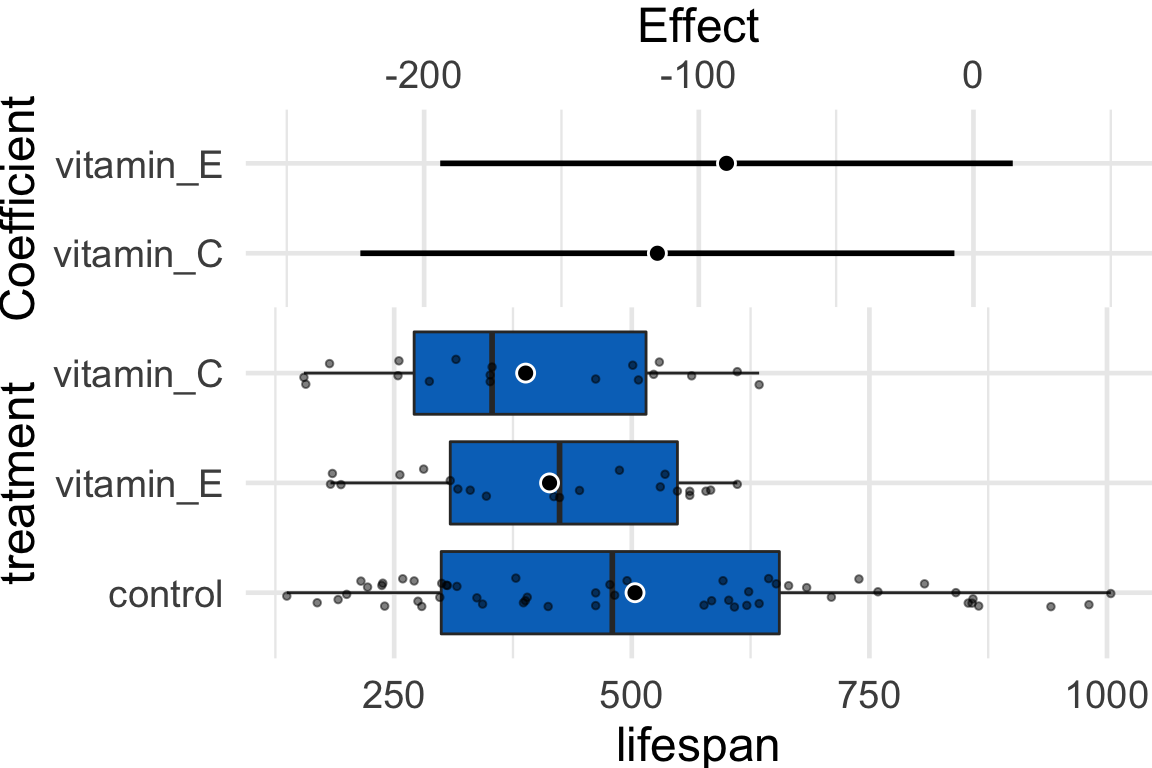
\includegraphics{Walker-elementary-statistical-modeling-draft_files/figure-latex/harrellplot-1.pdf}
\caption{\label{fig:harrellplot}HarrellPlot of the raw data, distribution,
and effects of the vole lifespan data.}
\end{figure}

The raw data, the distributions within treatment level, and the effects
(difference in means) of treatment can be combined into a single plot
that I call a Harrell plot (Figure \ref{fig:voles}). Notice that the
\emph{x}-axis and \emph{y} axes are flipped so that \(lifespan\) is on
the \emph{x}-axis. It is still the ``response'' or ``Y'' variable! The
Harrell plot contains two parts

\begin{enumerate}
\def\labelenumi{\arabic{enumi}.}
\tightlist
\item
  The bottom contains a \textbf{strip chart} (often called a ``dot
  plot'') of the raw response measures grouped by factor level.
  Superimposed over the strip chart is a \textbf{box plot} summarizing
  the distribution of each factor level. The line in the center of a box
  is the median \(lifespan\) for that group, the left and right edges of
  the box are the 25\% and 75\% quantiles of \(lifespan\) for that grop,
  and the lines extending to the left and right of the box are the
  ``whiskers'', which are the smallest and largest value within
  \(1.5 IQR\) (inter-quartile range, which is the interval bounded by
  box).
\item
  The top is a \textbf{forest plot} of the effects and the 95\% CI of
  the effects. For categorical \(X\), the effects could be model
  coefficients or treatment \textbf{contrasts}, which are differences in
  means between treatment levels. Model coefficients are a subset of
  possible treatment contrasts.
\end{enumerate}

The Harrell plot above shows the effects as model coefficients, which
(again!) are differences between the mean of the response in a specific
treatment level and the mean of the response in a reference level. Here
the reference level is the control group.

\subsubsection{In-text reporting}\label{in-text-reporting}

``The mean lifespan of cold-reared voles supplmented with vitamin E was
-89.9 days shorter than the mean lifespan for the control group (95\%
CI: -194.1, 14.3). The mean lifespan of cold-reared voles supplmented
with vitamin C was -115.1 days shorter than the mean lifespan for the
control group (95\% CI: -223.2, -6.9).

\subsubsection{Correct interpretation of the Confidence Interval is
key}\label{correct-interpretation-of-the-confidence-interval-is-key}

Remember, that the CI contains the range of parameter values that are
consistent with the data (in the sense that a t-test wouldn't reject the
hypothesis test). This means that a true value at the low end or the
high end of the CI is consistent with the data. Your technical
report/manuscript should discuss the consequences of this. For example,
A small, increase in lifespan is consistant with the Vitamin E but not
Vitamin C supplementation, if we use the 95\% CI as a pretty good range
for inferring ``consistent with''. Both a 223 day and a 7 day decrease
in lifespan are consistant with the Vitamin C effect. 223 days seems
like a huge effect, especially for a short lived vole. 7 days is
certainly a much smaller effect, but this doesn't mean that it doesn't
have important ecological, behavioral, or fitness consequences.

\section{Working in R}\label{working-in-r-1}

\subsection{\texorpdfstring{Exploring the relationship between \emph{Y}
and
\emph{X}}{Exploring the relationship between Y and X}}\label{exploring-the-relationship-between-y-and-x}

Questions

\begin{enumerate}
\def\labelenumi{\arabic{enumi}.}
\tightlist
\item
  Import the vole data from the Dryad repository as the data.table
  \texttt{vole\_wide}. Replace the spaces in the column labels with the
  underscore ``\_``.
\end{enumerate}

The data are in ``wide'' format. A pretty good script for for converting
these to long format is

\begin{Shaded}
\begin{Highlighting}[]
\NormalTok{vole_long <-}\StringTok{ }\KeywordTok{melt}\NormalTok{(vole_wide, }\DataTypeTok{measure.vars=}\KeywordTok{c}\NormalTok{(}\StringTok{"control"}\NormalTok{, }\StringTok{"vitamin_E"}\NormalTok{, }\StringTok{"vitamin_C"}\NormalTok{), }\DataTypeTok{variable.name=}\StringTok{"treatment"}\NormalTok{)}
\NormalTok{vole <-}\StringTok{ }\KeywordTok{na.omit}\NormalTok{(vole_long)}
\CommentTok{# melt is from reshape2 package and is a workhorse in R}
\CommentTok{# the resulting data frame has 3 stacked copies of the same rows}
\CommentTok{# na.omit removes the superfluous two extra sets of rows created by melt}
\CommentTok{# the more compact way to do this is combine the steps:}
\CommentTok{# vole <- na.omit(melt(vole_wide, measure.vars=c("control", "vitamin_E", "vitamin_C"))}
\CommentTok{# but I suggest two steps so you can see what melt does. This isn't the best example of using melt.}
\end{Highlighting}
\end{Shaded}

Use the ggpubr package to create a box plot, grouped by treatment, with
superimposed strip chart (``dots'')

Questions

\begin{enumerate}
\def\labelenumi{\arabic{enumi}.}
\setcounter{enumi}{1}
\tightlist
\item
  Do the response as a function of group look fairly normally
  distributed or are there red flags such as skewness, outliers, bimodal
  clusters, etc.
\item
  Is the direction of the effect consistent with the expected direction?
\end{enumerate}

\subsection{Fitting the model}\label{fitting-the-model}

As with a single, continuous \(X\), we fit the model using the
\texttt{lm} function and with the model formula of the form
\texttt{y\ \textasciitilde{}\ x}. Note that the R formula can use the
single categorical variable \(treatment\). The code underneath lm will
note that \(treatment\) is a factor with three levels and will
automatically create the two dummy variables noted above in the linear
model.

\begin{Shaded}
\begin{Highlighting}[]
\NormalTok{fit <-}\StringTok{ }\KeywordTok{lm}\NormalTok{(lifespan }\OperatorTok{~}\StringTok{ }\NormalTok{treatment, }\DataTypeTok{data=}\NormalTok{vole)}
\end{Highlighting}
\end{Shaded}

All of the same scripts to access the information in \texttt{fit} that
we used with the continuous \(X\) analysis are the same. For example,
the base R \texttt{summary} function gives the same information as in
the continuous \(X\) example.

Questions

\begin{enumerate}
\def\labelenumi{\arabic{enumi}.}
\setcounter{enumi}{3}
\tightlist
\item
  Review different output in the \texttt{summary} function and list
  which are useful and which are not so useful and why.
\end{enumerate}

Other useful functions on the lm object (``fit'') are
\texttt{coefficients(summary())}, \texttt{coef()} or
\texttt{coefficients()} and \texttt{confint}. Assigning the output of
these functions to an R object allows you to increase reproducibility.
For example, if I assign the coefficients to \texttt{b}

\begin{Shaded}
\begin{Highlighting}[]
\NormalTok{b <-}\StringTok{ }\KeywordTok{coef}\NormalTok{(fit)}
\end{Highlighting}
\end{Shaded}

then I can report these in R markdown text by embedding r code directly
in the text. For example, if I embed ``r
round(b{[}``treatmentvitamin\_E''{]}, 1)'' between a pair of single
accent characters, then r markdown inserts -89.9 into the rendered text.

\subsection{An introduction to
contrasts}\label{an-introduction-to-contrasts}

We often want to compare more than just the non-reference levels to the
reference level. For example, we might want to compare the effects of
the vitamin E supplementation to vitamin C supplementation. Or, we might
want to combine (or ``pool'') vitamin C and vitamin E levels effects
into a single ``anti-oxidant'' level and compare to the control. These
comparisons of means are called linear \textbf{contrasts}. The emmeans
package is a good package for obtaining contrasts for both simple linear
models computed with \texttt{lm} and for more complicated statistical
models. If you haven't already, download the emmeans package.

\begin{Shaded}
\begin{Highlighting}[]
\NormalTok{fit.em <-}\StringTok{ }\KeywordTok{emmeans}\NormalTok{(fit, }\DataTypeTok{spec=}\StringTok{"treatment"}\NormalTok{)}
\NormalTok{fit.em}
\end{Highlighting}
\end{Shaded}

\begin{verbatim}
##  treatment emmean   SE df lower.CL upper.CL
##  control      503 27.4 93      449      558
##  vitamin_E    413 44.8 93      325      502
##  vitamin_C    388 47.1 93      295      482
## 
## Confidence level used: 0.95
\end{verbatim}

The \texttt{emmeans()} function returns various estimated means,
depending on what is specified with the \texttt{spec=} parameter. Here
the grouping variable ``treatment'' is specified, so the means returned
are estimates of \(\mathrm{E}(lifespan | treatment)\), the modeled means
for each level of treatment. For this simple analysis, the modeled means
are simply the group means. Note that the default value returned is a
table with the standard error and 95\% confidence limits of the
estimates.

Let's use the emmeans object to get the contrasts for all combinations
of treatment levels.

\begin{Shaded}
\begin{Highlighting}[]
\KeywordTok{summary}\NormalTok{(}\KeywordTok{contrast}\NormalTok{(fit.em, }\DataTypeTok{method=}\StringTok{"revpairwise"}\NormalTok{, }\DataTypeTok{adjust=}\StringTok{"none"}\NormalTok{), }\DataTypeTok{infer=}\KeywordTok{c}\NormalTok{(}\OtherTok{TRUE}\NormalTok{, }\OtherTok{TRUE}\NormalTok{))}
\end{Highlighting}
\end{Shaded}

\begin{verbatim}
##  contrast              estimate   SE df lower.CL upper.CL t.ratio p.value
##  vitamin_E - control      -89.9 52.5 93     -194    14.31 -1.713  0.0900 
##  vitamin_C - control     -115.1 54.5 93     -223    -6.93 -2.113  0.0373 
##  vitamin_C - vitamin_E    -25.2 64.9 93     -154   103.81 -0.387  0.6993 
## 
## Confidence level used: 0.95
\end{verbatim}

I've sent to parameters to the contrast function and one to the summary
function

\begin{enumerate}
\def\labelenumi{\arabic{enumi}.}
\tightlist
\item
  method=``revpairwise''. \texttt{contrast} can create different
  combinations of differences between means. Here I've specified all
  pairwise differences (the ``rev'' reverses the order of the
  subtraction). Notice that the statistics (estimate, SE, etc) are equal
  to the same statistics for \(b_1\) and \(b_2\) of the linear model. I
  said earlier that these coefficients are contrasts!
\item
  adjust=``none''. In classical frequentist hypothesis testing, the
  p-value of a contrast in what are called ``post-hoc tests'' is
  adjusted to reflect ``multiple testing'' (more than one p-value is
  being computed). This adjustment is almost standard in biology, but
  the practice is hugely controversial. The concept of multiple testing
  is important, and we will return to this in a future chapter, but here
  I have chosen to show the unadjusted p-value. The reason is that I
  want the unadjusted confidence interval and the adjustment would
  adjust these as well. If deleted \texttt{adjust="none"} from the
  script, the contrast function would default to the \textbf{Tukey HSD}
  (Honestly Significant Difference) test. There are literally dozens and
  dozens of post-hoc tests, which largely reflects the misplaced
  emphasis on ``better'' \(p\)-values rather than parameter estimates
  and their uncertainty.
\item
  infer=c(TRUE, TRUE). This parameter controls what kind of inference to
  put in the table. The first value specifies the inclusion of the CI
  (emmeans uses ``CL'' for confidence limit), the second value specifies
  the inclusion of \(t\) and \(p\)-values.
\end{enumerate}

\subsection{Harrell plot}\label{harrell-plot}

\subsubsection{Installing the harrellplot
package}\label{installing-the-harrellplot-package}

The harrellplot package is available on github but not a cran repository
and, therefore, takes a little more work to install. To install a
package from a github repository, 1. load library(devtools) -- this may
need to be installed first using the R Studio Tools \textgreater{}
Install Packages\ldots{} tool 2. install harrellplot from github. In the
console, type

\texttt{install\_github("middleprofessor/harrellplot")}

\begin{enumerate}
\def\labelenumi{\arabic{enumi}.}
\setcounter{enumi}{2}
\tightlist
\item
  load the harrellplot package
\item
  harrellplot requires other packages including broom, Hmisc, car, lme4,
  and lmerTest. If you haven't installed these do. load these with the
  library() function at the start of your notebook.
\end{enumerate}

\subsubsection{Using harrellplot to make a nice, publishable plot of
treatment
effects}\label{using-harrellplot-to-make-a-nice-publishable-plot-of-treatment-effects}

In the console type `?harrellplot to see the many parameters. Unlike
ggplot2, variable names need to be specified with quotes in the
harrellplot function. The harrellplot function is a list with several
elements.

Here is the default plot

\begin{Shaded}
\begin{Highlighting}[]
\NormalTok{vole.harrellplot <-}\StringTok{ }\KeywordTok{harrellplot}\NormalTok{(}\DataTypeTok{x=}\StringTok{"treatment"}\NormalTok{, }\DataTypeTok{y=}\StringTok{"lifespan"}\NormalTok{, }\DataTypeTok{data=}\NormalTok{vole)}
\NormalTok{vole.harrellplot}\OperatorTok{$}\NormalTok{gg }\CommentTok{# gg is the plot object}
\end{Highlighting}
\end{Shaded}

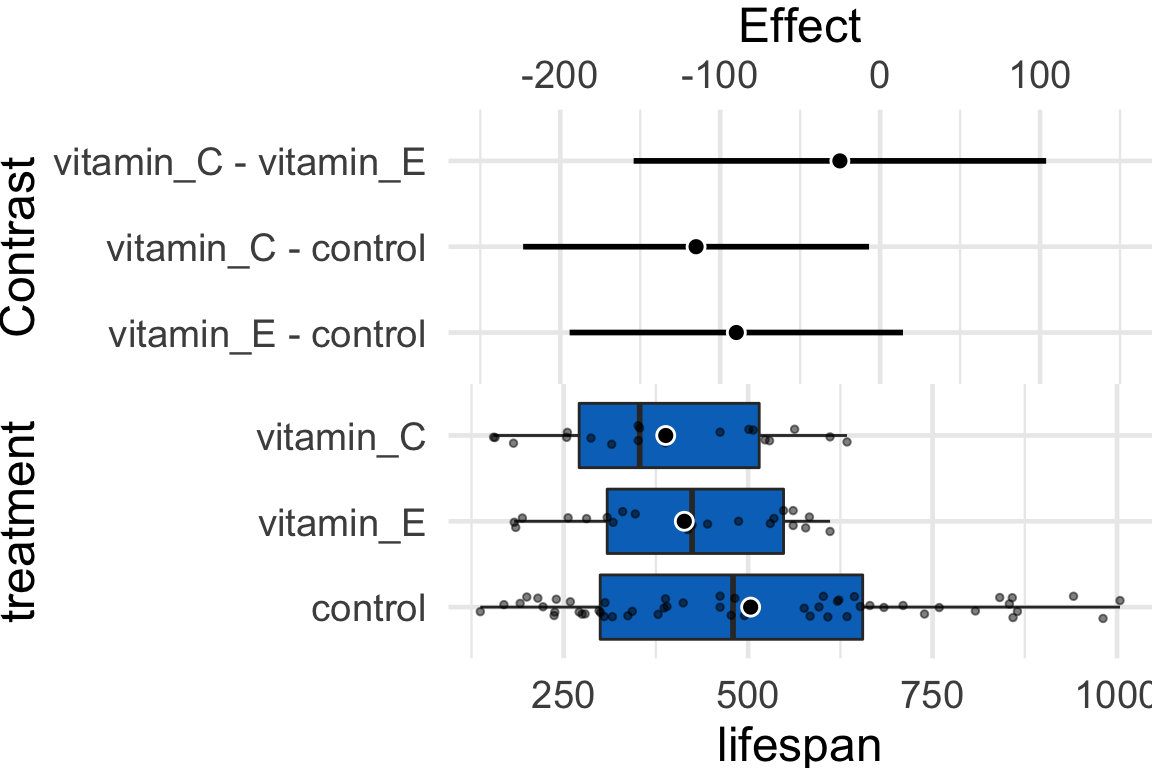
\includegraphics{Walker-elementary-statistical-modeling-draft_files/figure-latex/unnamed-chunk-21-1.pdf}

\chapter{Model Checking}\label{model-checking-1}

\begin{Shaded}
\begin{Highlighting}[]
\CommentTok{# a function to transform a vector into quantiles}
\CommentTok{# not if the data are 1:n then the output is "rankits"}
\NormalTok{quantilize_}\DecValTok{1}\NormalTok{ <-}\StringTok{ }\ControlFlowTok{function}\NormalTok{(x)\{}
  \CommentTok{# this is the ppoints(x) function}
\NormalTok{  m <-}\StringTok{ }\KeywordTok{length}\NormalTok{(x)}
\NormalTok{  s <-}\StringTok{ }\KeywordTok{trunc}\NormalTok{(}\KeywordTok{rank}\NormalTok{(x))}
\NormalTok{  a <-}\StringTok{ }\KeywordTok{ifelse}\NormalTok{(m }\OperatorTok{<=}\StringTok{ }\DecValTok{10}\NormalTok{, }\DecValTok{3}\OperatorTok{/}\DecValTok{8}\NormalTok{, }\DecValTok{1}\OperatorTok{/}\DecValTok{2}\NormalTok{)}
\NormalTok{  q <-}\StringTok{ }\NormalTok{(s}\OperatorTok{-}\NormalTok{a)}\OperatorTok{/}\NormalTok{(m }\OperatorTok{+}\StringTok{ }\NormalTok{(}\DecValTok{1}\OperatorTok{-}\NormalTok{a) }\OperatorTok{-}\StringTok{ }\NormalTok{a)}
  \KeywordTok{return}\NormalTok{(q)}
\NormalTok{\}}
\end{Highlighting}
\end{Shaded}

\section{Do coefficients make numeric
sense?}\label{do-coefficients-make-numeric-sense}

\section{All statistical analyses should be followed by model
checking}\label{all-statistical-analyses-should-be-followed-by-model-checking}

We us a linear model (or statistical model more generally) to infer
effects or predict future outcomes. Our inference is uncertain. Given
some modeling assumptions, we can quantify this uncertainty with
standard errors, and from these standard errors we can compute
confidence intervals and \emph{p}-values. It is good practice to use a
series of \textbf{diagnostic plots}, diagnostic statistics, and
simulation to check how well the data approximate the fit model and
model assumptions. \textbf{Model checking} is used to both check our
subjective confidence in the modeled estimates and uncertainty and to
provide empirical evidence for subjective decision making in the
analysis workflow.

\textbf{NHST blues} -- Researchers are often encouraged by textbooks,
colleagues, or the literature to test the assumptions of a \emph{t}-test
or ANOVA with formal hypothesis tests of distributions such as a
Shaprio-Wilks test of normality or a Levine test of homogeneity. In this
strategy, an alternative to the \emph{t}-test/ANOVA is used if the
distribution test's p-value is less than some cut-off (such as 0.05).
Common alternatives include 1) transformations of the response to either
make it more normal or the variances more homogenous, 2) implementation
of alternative tests such as a Mann-Whitney-Wilcoxon (MWW) test for
non-normal data or a Welch \emph{t}-test/ANOVA for heterogenous
variances. The logic of a test of normality or homogeneity before a
\emph{t}-test/ANOVA isn't consistent with frequentist thinking because
the failure to reject a null hypothesis does not mean the null
hypothesis is true. We shouldn't conclude that a sample is ``normal'' or
that the variances are ``homogenous'' because a distributional test's
\emph{p}-value \textgreater{} 0.05. But, maybe we should of the
distributional pre-test as an ``objective'' model check? The logic of
this objective decision rule suffers from several issues.
\textbf{First}, the subsequent \emph{p}-value of the \emph{t}test/ANOVA
test is not valid because this \emph{p}-value is the long-run frequency
of a test-statistic as large or larger than the observed statistic
conditional on the null -- not conditional on the subset of nulls with
\(p > 0.05\) in the distribution test. \textbf{Second}, real data are
only approximately normal; with small \(n\), it will be hard to reject
the null of a normal distribution because of low power, but, as \(n\)
increses, a normality test will reject any real dataset. \textbf{Third},
and most importantly, our analysis should follow the logic of our goals.
If our goal is the estimation of effects, we cannot get meaningful
estimates from a non-parametric test (with a few exceptions) or a
transformed response, as these methods are entirely about computing a
``correct'' \emph{p}-value. Good alternatives to classic non-parametric
tests and transformations are bootstrap estimates of confidence limits,
permutation tests, and generalized linear models.

\section{Linear model assumptions}\label{linear-model-assumptions}

Assumptions of a linear model concern the distribution of the ``random
draw'' in the underlying statistical model. Again, in the random error
specification of a linear model

\begin{align}
Y &= \beta_0 + \beta_1 X + \varepsilon\\
\varepsilon &\sim N(0, \sigma)
\label{eq:model-checking-spec1}
\end{align}

the random draw (the ``error'') is from a normal distribution with mean
zero and standard deviation \(\sigma\). In the random conditional
response specification

\begin{align}
y_i &\sim N(\mu_i, \sigma)\\
\mathrm{E}(Y|X) &= \mu\\
\mu_i &= \beta_0 + \beta_1 x_i
\label{eq:model-checking-spec2}
\end{align}

the random draw is a value drawn from a normal distribution with mean
\(\mu_i = \beta_0 + \beta_1 x_i\) and variance \(\sigma^2\). Any
inference about the parameter \(\beta_1\) (such as confidence intervals
or hypothesis tests) assumes that the these distributions are IID Normal
where IID is \textbf{independent and identically distributed} and Normal
refers to the Normal (or Gaussian) distribution.

\begin{enumerate}
\def\labelenumi{\arabic{enumi}.}
\tightlist
\item
  Independent means that the error for one case cannot be predicted from
  the error of any other case. This lack of independence creates
  \emph{correlated error}. There are lots or reasons that errors might
  be correlated. If individuals are measured both within and among
  cages, or tanks, or plots, or field sites, then we'd expect the
  measures within the same unit (cage, tank, plot, site) to err from the
  model in the same direction because of environmental features shared
  by individuals within the unit but not by individuals in other units.
  Multiple measures within experimental units create ``clusters'' of
  error. Lack of independence or clustered error can be modeled using
  models with \textbf{random effects}. These models go by many names
  including linear mixed models (common in Ecology), hierarchical
  models, multilevel models, and random effects models. A linear mixed
  model is a variation of model \eqref{eq:model-checking-spec1}.
\end{enumerate}

\textbf{tl;dr} -- Measures taken within the same individual over time
(\emph{repeated measures}) are correlated and are common in all areas of
biology. In ecology and evolutionary studies, measures that are taken
from sites that are closer together or measures taken closer in time or
measures from more closely related biological species will tend to have
more similar error than measures taken from sites that are further apart
or from times that are further apart or from species that are less
closely related. Space and time and phylogeny create \textbf{spatial,
temporal, and phylogenetic autocorrelation}. Correlated error due to
space or time or phylogeny can be modeled with \textbf{Generalized Least
Squares} (GLS) models. A GLS model is a variation of model
\eqref{eq:model-checking-spec1}.

\begin{enumerate}
\def\labelenumi{\arabic{enumi}.}
\setcounter{enumi}{1}
\item
  Identical means that the errors are ``drawn'' from the same
  distribution. Since the model is a linear model, this distribution is
  a Normal distribution with mean zero and variance \(\sigma^2\). A
  consequence of ``identical'' is that the error variance is
  \textbf{homoskedastic}, or constant, or independent of \(X\). If the
  error variance differs among the \(X\) then the errors are
  \textbf{heteroskedastic}. Many biological processes generate data in
  which the error is a function of the mean. For example, measures of
  biological variables that grow, such as lengths of body parts or
  population size, have variances that ``grow'' with the mean. Or,
  measures of counts, such as the number of cells damaged by toxin, the
  number of eggs in a nest, or the number of mRNA transcripts per cell
  have variances that are a function of the mean. Both growth and count
  measures can sometimes be reasonably modeled using a linear model but
  more often, they are better modeled using a \textbf{generalized linear
  model} (GLM), which is an extension of a linear model. Heteroskedasitc
  error arising for other reasons, both biological and experimental, can
  be modeled with Generalized Least Squares (GLS) or with linear mixed
  models..
\item
  Normal (Gaussian) error means that 1) the response is continuous and
  2) the probability of sampling an individual measuring 0.5 units below
  the population mean is the same as the probability of sampling an
  individual measuring 0.5 units above the population mean. Counts
  (number of cells, number of eggs, number of mRNA transcripts) and
  binary responses (sucessful escape or sucessful infestation of host)
  are not continous and often often have asymmetric probablity
  distributions that are skewed to the right and while sometimes both
  can be reasonably modeled using a linear model they are more often
  modeled using a \textbf{generalized linear model} (GLM), which, again,
  is an extension of the linear model in equation
  \eqref{eq:model-checking-spec1}.
\end{enumerate}

\section{Diagnostic plots use the residuals from the model
fit}\label{diagnostic-plots-use-the-residuals-from-the-model-fit}

\subsection{Residuals}\label{residuals}

A residual of a statistical model is \(y_i - \hat{y}_i\). Remember that
\(\hat{y}_i\) is the predicted value of \(Y\) when \(X\) has the value
\(x_i\) (compaactly written as \(X=x_i\)). And remember that
\(\hat{y}_i\) is the estimate of \(\mu_i\). For linear models (but not
generalized linear models), the residuals of the fit model are estimates
of the \(\varepsilon\) in equation \eqref{eq:model-checking-spec1}. This
\emph{is not} true for generalized linear models because GLMs are not
specified using \eqref{eq:model-checking-spec1}.

\textbf{Alert} A common misconception is that inference from a linear
model assumes that the \emph{response} (the measured \(Y\)) is IID
Normal. This is wrong. Either specification of the linear model shows
precisely why this conception is wrong. Model
\eqref{eq:model-checking-spec1} explicitly shows that it is the error that
has the normal distribution -- the distribution of \(Y\) is a mix of the
distribution of \(X\) and that of the error. A more general way of
thinking about the assumed distribution uses the specification in model
\eqref{eq:model-checking-spec2}, which shows that it is the
\emph{conditional} response that is assumed to be IID normal. Remember,
a conditional response (\(y_i\)) is a random draw from the infinite set
of responses at a given value of \(X\).

Let's look at the distribution of residuals versus the response for a
hypothetical experiment with a single, categorical \(X\) variable (the
experimental factor) with two levels (``Cn'' for control and ``Tr'' for
treatment). The true parameters are \(\beta_0 = 10\) (the true mean for
the control group, or \(\mu_{0}\)), \(\beta_1=4\) (the difference
between the true mean for the treatment minus the true mean for the
control, or \(\mu_1 - \mu_0\)), and \(\sigma = 2\) (the error standard
deviation).

\begin{figure}
\centering
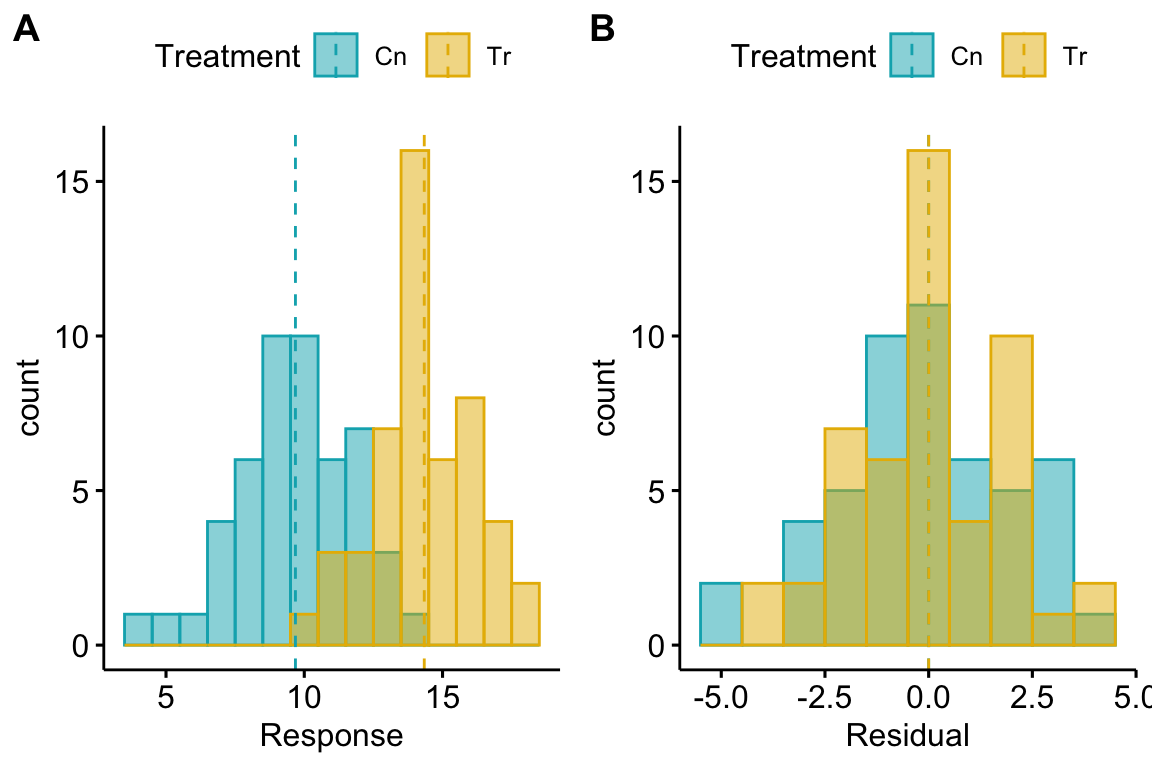
\includegraphics{Walker-elementary-statistical-modeling-draft_files/figure-latex/model-check-histogram, model-check-residuals1-1.pdf}
\caption{(\#fig:model-check-histogram, model-check-residuals1)Histogram
of the (A) response, showing with modes near the true means of each
group and (B) residuals, with a mode for both groups at zero.}
\end{figure}

The plot above shows a histogram of the response (A) and residuals (B).
In the plot of the response, the mode (the highest bar, or bin with the
most cases) includes true mean for each group. And, as expected given
\(\beta_1=4\), the modes of the two groups are 4 units apart. It should
be easy to see from this plot that the response does not have a normal
distribution. Instead, it is distincly bimodal. But the distribution of
the response \emph{within} each level looks like these are drawn from a
normal distribution -- and it should. In the plot of the residuals, the
values of both groups are shifted so that the mean of each group is at
zero. The consequence of the shift is that the combined set of residuals
does look like it is drawn from a Normal distribution.

The two plots suggest two different approaches for model checking.
First, we could examine the responses within each level of the
experimental factor. Or, second, we could examine the residuals of the
fit model, ignoring that the residuals come from multiple groups. The
first is inefficient because it requires as many checks as there are
levels in the factor. The second requires a single check.

\textbf{Alert} Some textbooks that recommend formal hypothesis tests of
normality recommend the inefficient, multiple testing on each group
separately. This isn't wrong, it's just more work than it needs to be
and also suffers from ``multiple testing''.

\subsection{A Normal Q-Q plot is used to check
normality}\label{a-normal-q-q-plot-is-used-to-check-normality}

A Normal Q-Q plot of the residuals can be used to check how closely the
residuals approximate a normal distribution. A Normal Q-Q plot is a
scatterplot of

\begin{enumerate}
\def\labelenumi{\arabic{enumi}.}
\tightlist
\item
  \textbf{sample quantiles} on the \emph{y} axis. The sample quantiles
  is the vector of \(N\) residuals in rank order, from smallest (most
  negative) to largest (most positive). Sometimes this vector is
  standardized (doing this makes not difference to the interpretation of
  the Q-Q plot).
\item
  \textbf{standard normal quantiles} on the \emph{x} axis. This is the
  vector of standard normal quantiles given \(N\) elements in the
  vector.
\end{enumerate}

\textbf{Stats 101} A quantile is the value of a distribution that is
greater than \(p\) percent of the values in the distribution. The 2.5\%
quantile of a uniform distribution from 0 to 1 is 0.025. The 2.5\%
quantile of a standard normal distribution is -1.96 (remember that 95\%
of the values in a standard normal distribution are between -1.96 and
1.96). The 50\% quantile of a uniform distribution is 0.5 and the 50\%
quantile of a standard normal distribution is 0.0 (this is the median of
the distribtion -- 50\% of the values are smaller and 50\% of the values
are larger).

\textbf{Stats 201} A Q-Q plot more generally is a scatter plot of two
vectors of quantiles either of which can come from a sample or a
theoretical distribution. In the GLM chapter, the text will introduce
Q-Q plots of residual quantiles transformed to have an expected uniform
distribution. These are plotted against theoretical uniform quantiles
from 0 to 1.

If the sampled distribution closely approximates a normal distribution,
the scatter should fall along a line from the bottom, left to the top,
right of the plot. The interpretation of a normal Q-Q plot is enhanced
with a line of ``expected values'' of the sample quantiles if the sample
residuals are drawn from a normal distribution. The closer the sample
quantiles are to the line, the more closely the residuals approximate a
normal distribution. Because of sampling, the sampled values always
deviate from the line, especially at the ends. If the sample was drawn
from a normal distribution, these deviations should be small if the
sample size is big, but can be more pronounced with a small sample size.
This makes it hard to have much confidence in the ``normality'' of a
small sample.

Let's have a look at a Normal Q-Q plot of the residuals of the fake data
generated above.

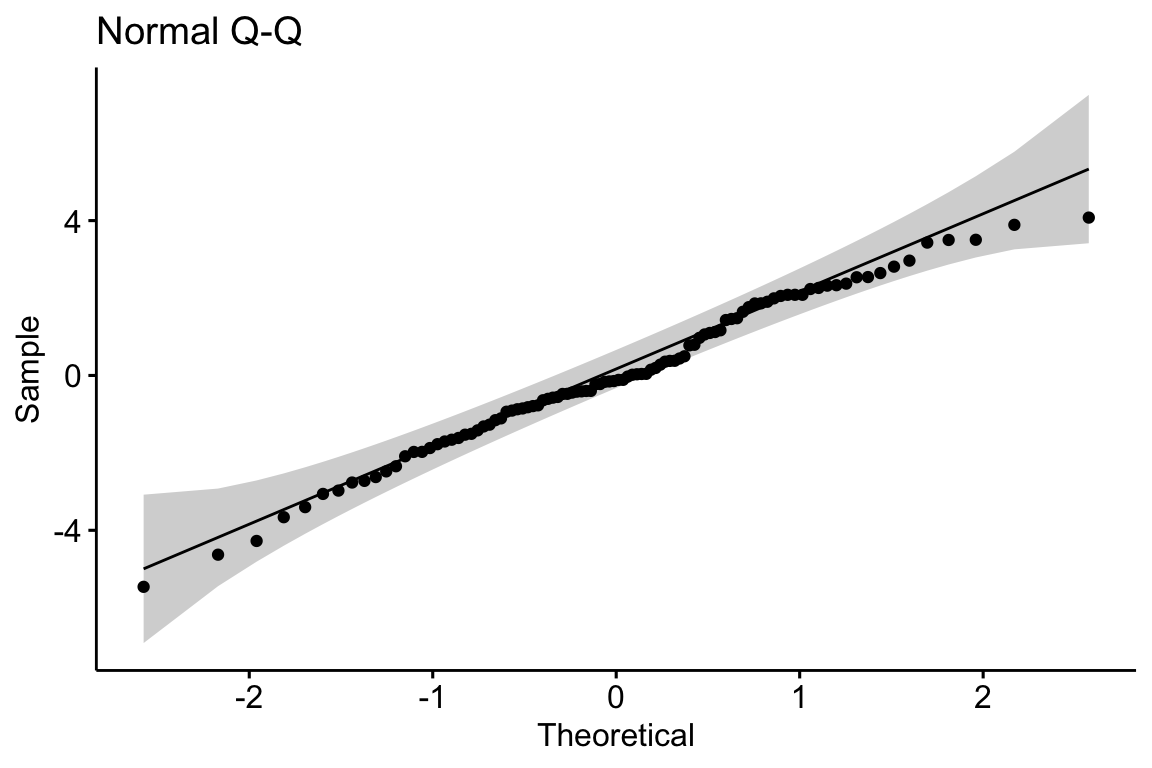
\includegraphics{Walker-elementary-statistical-modeling-draft_files/figure-latex/model-check-normal-qq-1.pdf}

Rules of a Q-Q plot

At the small end of the distribution (bottom-left), the sample values
are a bit more negative than expected, which means the left tail is a
bit extended. At the large end (upper-right), the sample values are, a
bit less positive than expected, which means the right tail is a bit
shortened. Should we fit a different model given these deviations? To
answer this, we look look at the shaded area, which represents the range
of expected deviations from expectation (the line) given the sample
size. Clearly the deviations are within this range.

Now let's look at simulated samples drawn from non-normal distributions
to identify their characteristic deviations.

\subsubsection{Right skewed}\label{right-skewed}

Many biological measures are from a distribution with long, right tails
(right skewed). Examples include many count variables (number of eggs in
a clutch, number of cells colonized by a parasite), and measures of
time, weight, or length. What is common to all of these is unconstrained
upper bounday but a constrained lower boundary at or above zero (A nest
might have zero but eggs. The weight of a fat depot must be greater than
zero but the weight of a specific species of fish in a trawl catch might
be zero).

A long right tail of conditional responses creates a characteristic
positive deviation of the largest quantiles in a Normal Q-Q plot of the
residuals from a linear model. Positive deviations at the upper end
indicate larger values than expected given a normal distribution. This
is the signature of the residuals of a linear model fit to right skewed
data.

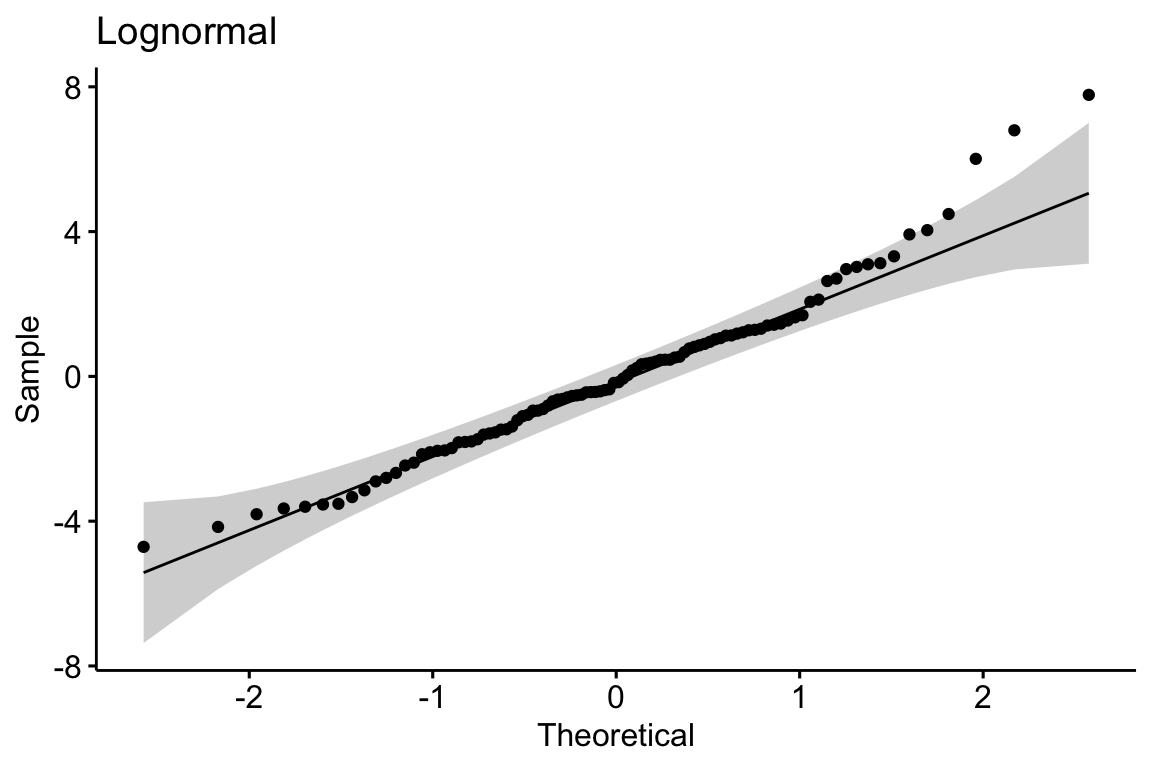
\includegraphics{Walker-elementary-statistical-modeling-draft_files/figure-latex/model-check-lognormal-1.pdf}

A continous response with a right skewed distribution can be modeled
with a generalized linear model using a lognormal or gamma distribution.
A count response can be modeled with a generalized linear model using a
Poisson, quasi-Poisson, or negative binomial distribution (Chapter xxx).

\subsubsection{Excess zeroes}\label{excess-zeroes}

Count data often have an excess of zeroes (for example a lake with no
nests or a host with no parasites), resulting in positive deviations
(closer to zero) at the lower end of the quantile range.

\begin{Shaded}
\begin{Highlighting}[]
\CommentTok{# zero inflated}
\NormalTok{mu_pois <-}\StringTok{ }\FloatTok{2.7}
\NormalTok{beta_pois <-}\StringTok{ }\DecValTok{2}
\NormalTok{p_zero <-}\StringTok{ }\FloatTok{0.3}

\NormalTok{fd.zipois <-}\StringTok{ }\KeywordTok{data.table}\NormalTok{(}
  \DataTypeTok{Treatment=}\KeywordTok{rep}\NormalTok{(}\KeywordTok{c}\NormalTok{(}\StringTok{"Cn"}\NormalTok{, }\StringTok{"Tr"}\NormalTok{), }\DataTypeTok{each=}\NormalTok{n),}
  \DataTypeTok{Response=}\KeywordTok{c}\NormalTok{(SpiecEasi}\OperatorTok{::}\KeywordTok{rzipois}\NormalTok{(n, }\DataTypeTok{lambda =}\NormalTok{ mu_pois, }\DataTypeTok{pstr0 =}\NormalTok{ p_zero), SpiecEasi}\OperatorTok{::}\KeywordTok{rzipois}\NormalTok{(n, }\DataTypeTok{lambda =}\NormalTok{ (mu_pois}\OperatorTok{+}\NormalTok{beta_pois), }\DataTypeTok{pstr0 =}\NormalTok{ p_zero))}
\NormalTok{)}
\NormalTok{m1 <-}\StringTok{ }\KeywordTok{lm}\NormalTok{(Response }\OperatorTok{~}\StringTok{ }\NormalTok{Treatment, }\DataTypeTok{data=}\NormalTok{fd.zipois)}
\NormalTok{fd.zipois[, Residual}\OperatorTok{:}\ErrorTok{=}\KeywordTok{residuals}\NormalTok{(m1)]}
\NormalTok{gg1.zipois <-}\StringTok{ }\KeywordTok{gghistogram}\NormalTok{(}\DataTypeTok{data=}\NormalTok{fd.zipois, }\DataTypeTok{x =} \StringTok{"Response"}\NormalTok{,}
                          \DataTypeTok{color=}\StringTok{"Treatment"}\NormalTok{, }\DataTypeTok{fill=}\StringTok{"Treatment"}\NormalTok{,}
                          \DataTypeTok{add =} \StringTok{"mean"}\NormalTok{, }\DataTypeTok{rug =} \OtherTok{FALSE}\NormalTok{,}
                          \DataTypeTok{bins=}\DecValTok{9}\NormalTok{,}
                          \DataTypeTok{palette =} \KeywordTok{c}\NormalTok{(}\StringTok{"#00AFBB"}\NormalTok{, }\StringTok{"#E7B800"}\NormalTok{)}
\NormalTok{)}

\NormalTok{gg3.zipois <-}\StringTok{ }\KeywordTok{ggqqplot}\NormalTok{(}\DataTypeTok{data=}\NormalTok{fd.zipois, }\DataTypeTok{x =} \StringTok{"Residual"}\NormalTok{, }\DataTypeTok{title=}\StringTok{"zero-inflated poisson"}\NormalTok{)}

\NormalTok{gg3.zipois}
\end{Highlighting}
\end{Shaded}

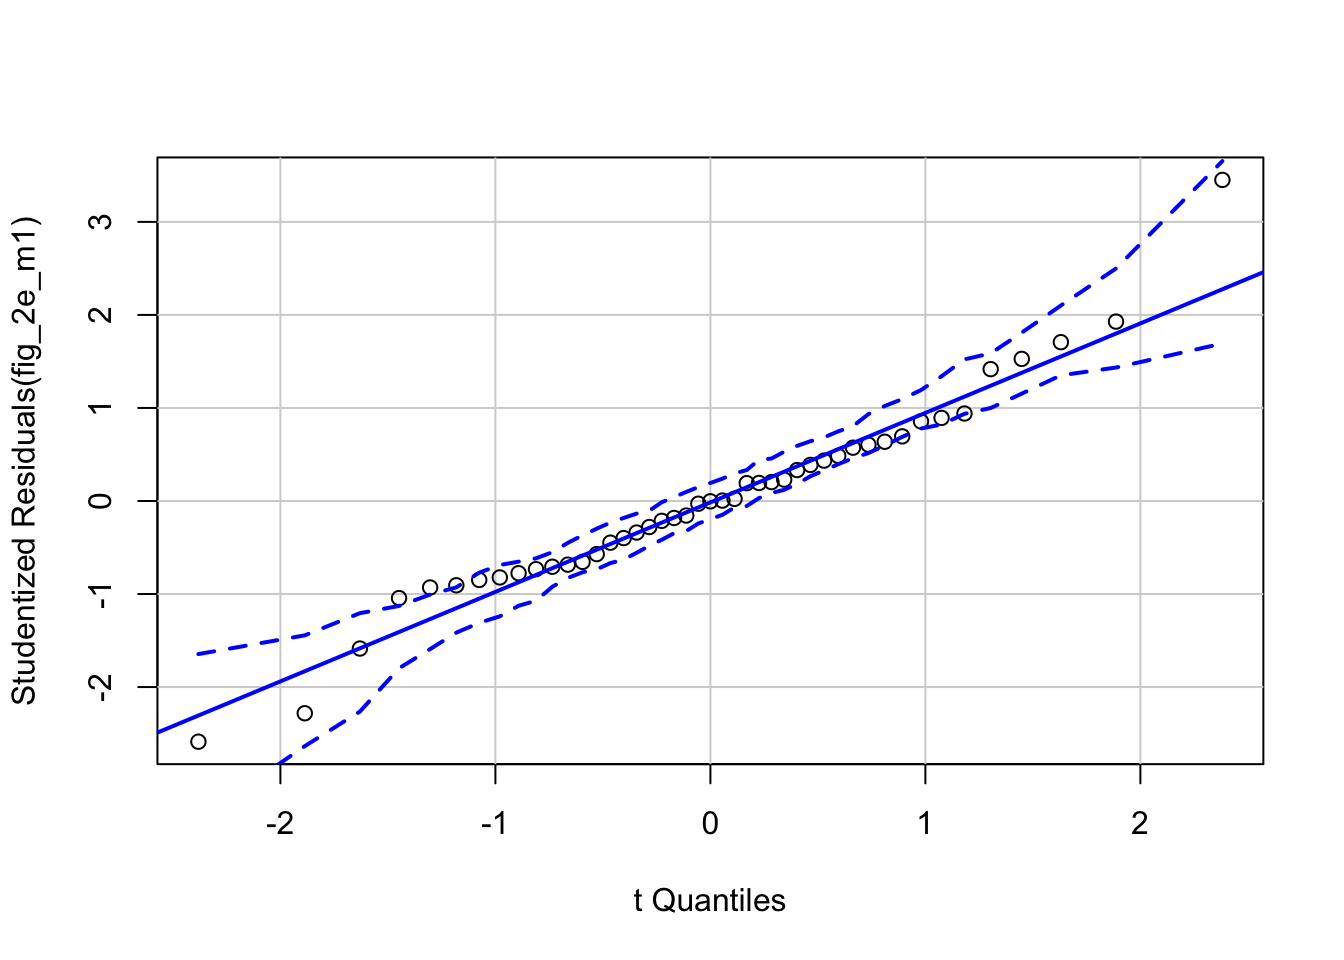
\includegraphics{Walker-elementary-statistical-modeling-draft_files/figure-latex/unnamed-chunk-22-1.pdf}

\subsubsection{Constrained lower and upper
bounds}\label{constrained-lower-and-upper-bounds}

Proportions are constrained to values between zero and one. A proportion
can have a distribution that approximates a normal distribution if the
mean is near 0.5 and the standard deviation is small. But, more
generally, proportions can have distributions with diverse shapes.

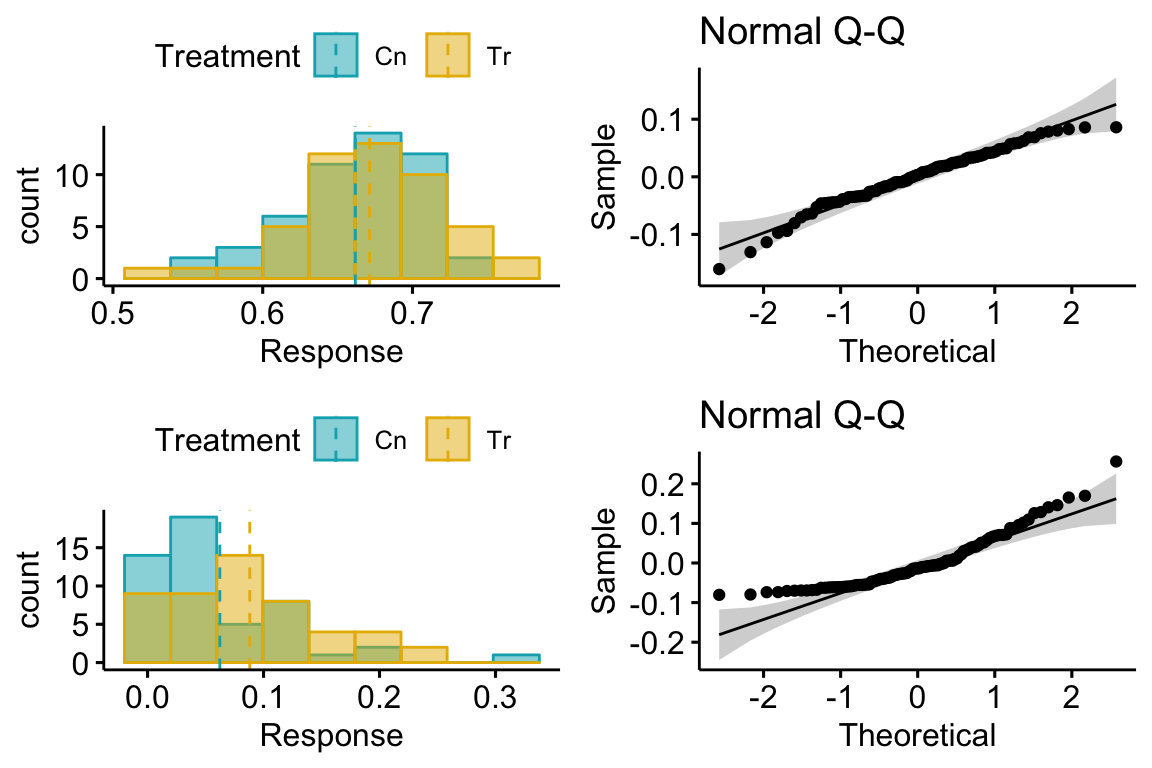
\includegraphics{Walker-elementary-statistical-modeling-draft_files/figure-latex/model-check-proportions-1.pdf}

\subsubsection{Binary responses}\label{binary-responses}

\subsection{Outliers - an outlier is a point that is highly unexpected
given the modeled
distribution.}\label{outliers---an-outlier-is-a-point-that-is-highly-unexpected-given-the-modeled-distribution.}

\section{Model checking
homoskedasticity}\label{model-checking-homoskedasticity}

\section{Model checking independence - hapiness adverse
example.}\label{model-checking-independence---hapiness-adverse-example.}

\section{Using R}\label{using-r}

\chapter{Model Fitting and Model Fit
(OLS)}\label{model-fitting-and-model-fit-ols}

\section{Least Squares Estimation and the Decomposition of
Variance}\label{least-squares-estimation-and-the-decomposition-of-variance}

The linear models in the last chapter and for much of this book are fit
to data using a method called ``ordinary least squares'' (OLS). This
chapter explores the meaning of OLS and related statistics, including
\(R^2\), as well as some alternative methods for bivariate regression.

\section{OLS regression}\label{ols-regression}

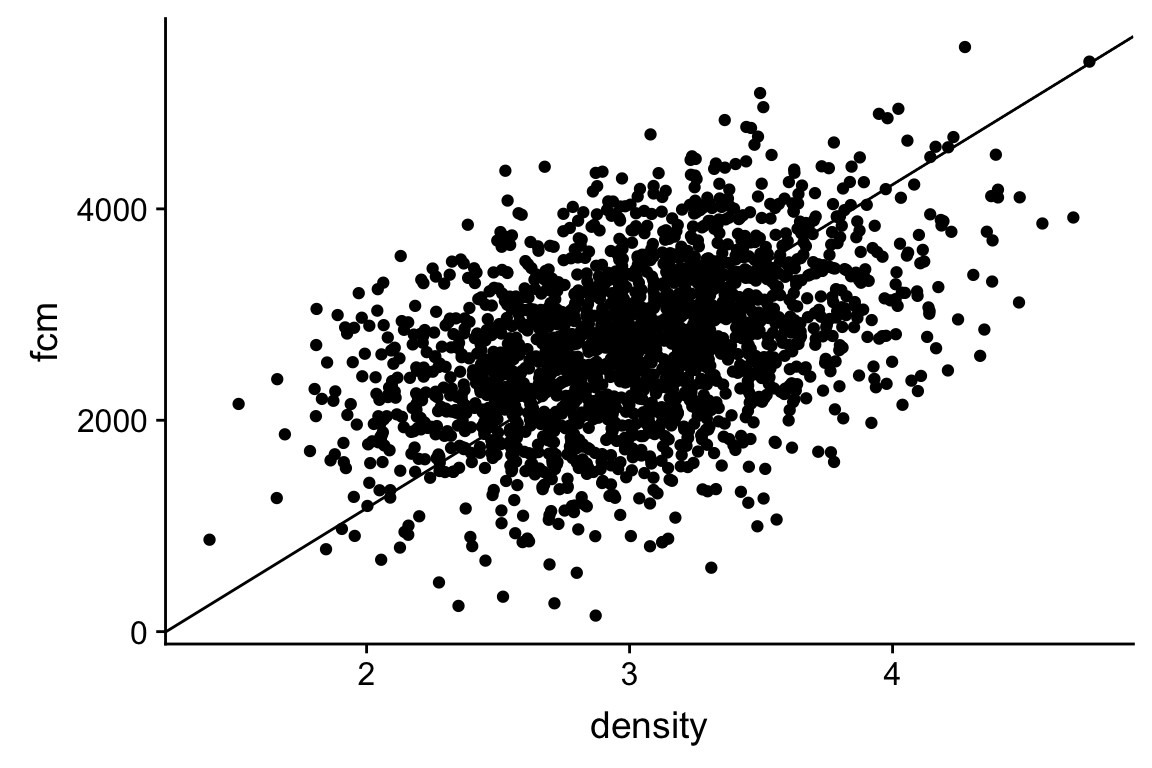
\includegraphics{Walker-elementary-statistical-modeling-draft_files/figure-latex/fake-data-ma-1.pdf}

The fake data illustrated in the scatterplot above (Figure
\ref{fig:fake-data-ma}) were modeled to look something like the squirrel
fecal cortisol metabolite data in the previous chapter. If a typical
student is asked to draw a regression line through the scatter, they
typically draw a line similar to that in Figure \ref{fig:fake-data-ma}.
This line is not the OLS regression line but the major axis of an elipse
that encloses the scatter of points--that students invariably draw this
line suggests that the brain interprets the major axis of an elliptical
scatter of points as a trend (This major axis line is an alternative
method for estimating a slope and is known as standard major-axis
regression. More about this at the end of this chapter.)

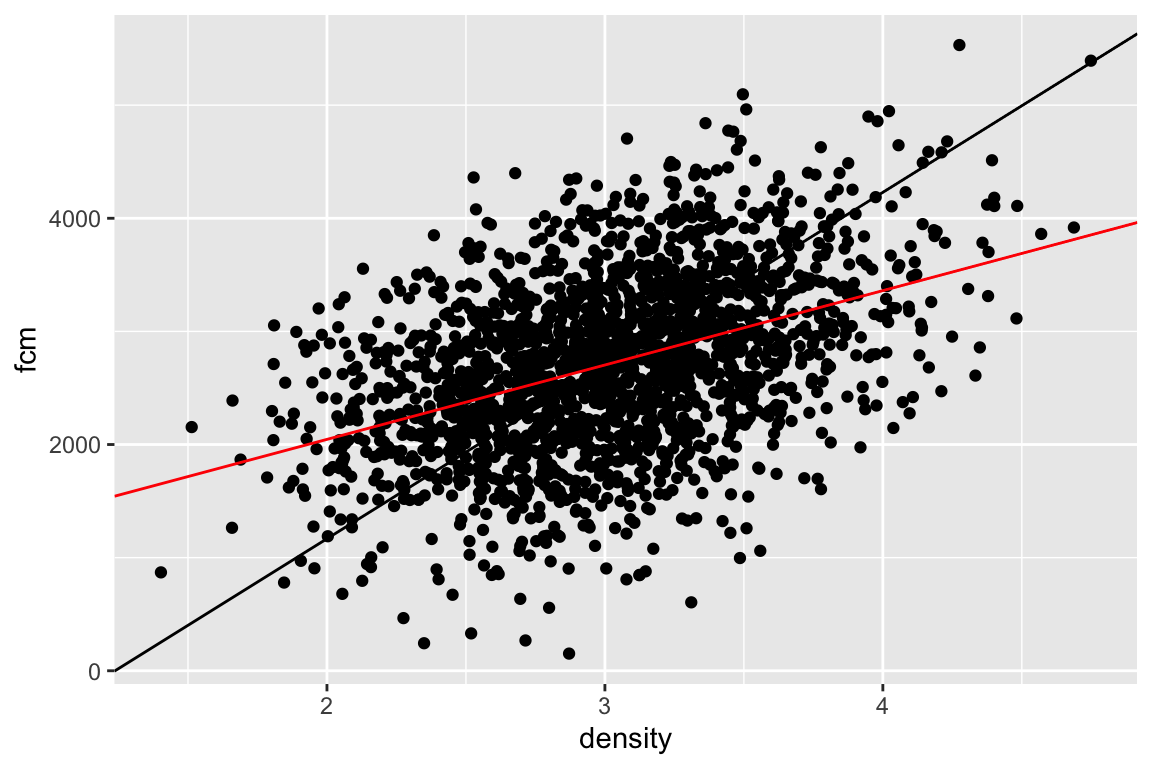
\includegraphics{Walker-elementary-statistical-modeling-draft_files/figure-latex/fake-data-ols-1.pdf}

The OLS regression line is the red line in Figure
\ref{fig:fake-data-ols} -- the standard major axis line is left for
comparison). The OLS regression line

\begin{enumerate}
\def\labelenumi{\arabic{enumi}.}
\tightlist
\item
  passes through the bivariate mean (\(\bar{x}\), \(\bar{y}\)) of the
  scatter, and
\item
  minimizes the sum of the squared deviations from each point to it's
  modeled value \(\sum{(y_i - \hat{y}_i)^2}\)
\end{enumerate}

There are an infinite number of lines that pass through the bivariate
mean (think of anchoring a line at the bivariate mean and spinning it).
The OLS line is the line that minimizes the squared (vertical)
deviations (``least squares'').

For a bivariate regression, the slope (coefficient \(b_1\) of \(X\)) of
the OLS model fit is computed by

\begin{equation}
b_1 = \frac{\mathrm{COV}(X, Y)}{\mathrm{VAR}(X)}
\end{equation}

This equation is worth memorizing. We will generalize this into a more
flexible equation in a few chapters.

\section{\texorpdfstring{How well does the model fit the data? \(R^2\)
and ``variance
explained''}{How well does the model fit the data? R\^{}2 and variance explained}}\label{how-well-does-the-model-fit-the-data-r2-and-variance-explained}

Let's switch to real data.

\begin{enumerate}
\def\labelenumi{\arabic{enumi}.}
\tightlist
\item
  Source: Dryad Digital Repository.
  \url{https://doi.org/10.5061/dryad.056r5}
\item
  File: ``Diet-shift data.xls''
\end{enumerate}

Fish require arachidonic acid (ARA) and other highyly unsaturated fatty
acids in their diet and embryo and yolk-stage larvae obtain these from
yolk. Fuiman and Faulk (xxx) designed an experiment to investigate if
red drum (\emph{Sciaenops ocellatus}) mothers provision the yolk with
ARA from recent dietary intake or from stored sources in somatic
tissues. The data below are from experiment 8. The \emph{x}-axis is the
days since a diet shift to more and less ARA (\(days\)) and the
\emph{y}-axis is the ARA content of the eggs (\(ARA\)).

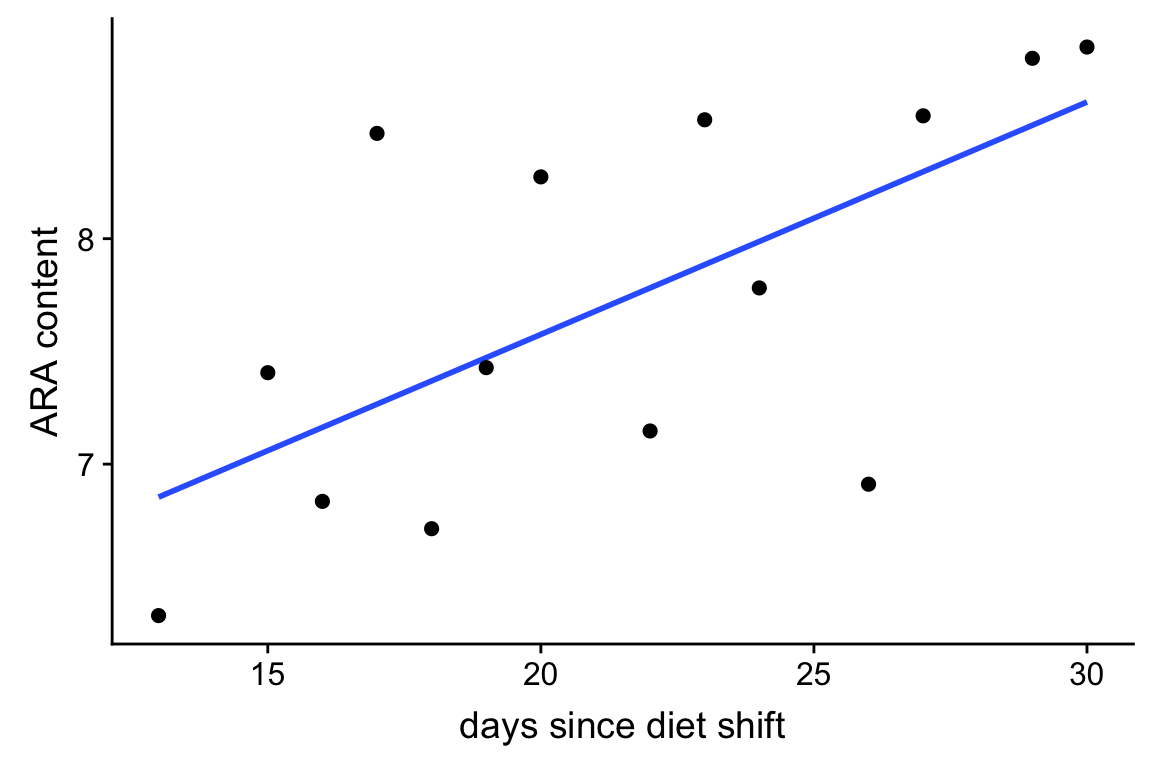
\includegraphics{Walker-elementary-statistical-modeling-draft_files/figure-latex/egg-data-1.pdf}

The statistic \(R^2\) is a measure of the fit of a model to data. The
\(R^2\) for the fit of the egg data is 0.42. \(R^2\) is the fraction of
two variances \(\frac{\mathrm{VAR}(Model)}{\mathrm{VAR}(Y)}\), or, the
fraction of the variance of \(Y\) ``explained by the model.'' The value
of \(R^2\) ranges from zero (the fit cannot be any worse) to one (the
fit is ``pefect'').

To understand \(R^2\), and its computation, a bit more, let's look at
three kinds of deviations.

\begin{figure}
\centering
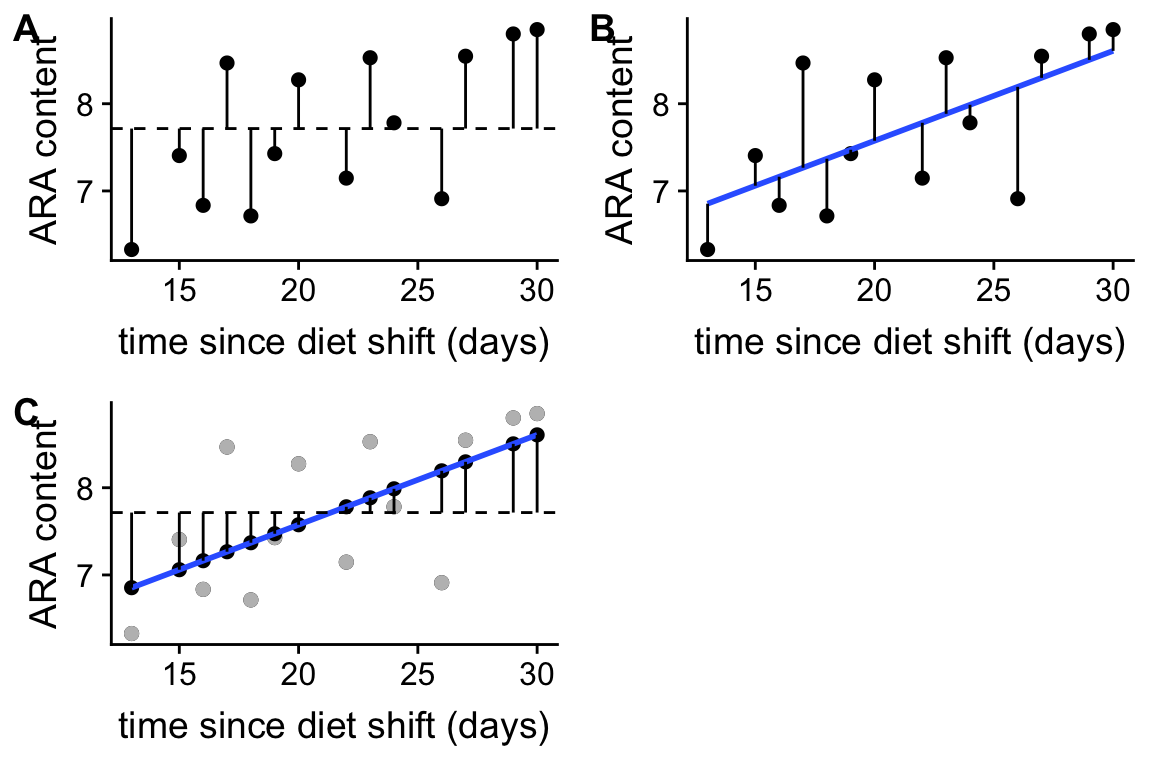
\includegraphics{Walker-elementary-statistical-modeling-draft_files/figure-latex/ols-deviations-1.pdf}
\caption{\label{fig:ols-deviations}Three kinds of deviations from a fit
model. A. Deviations of the measured values from the mean. These are in
the numerator of the equation of the sample variance. The dashed line is
the mean ARA content. B. Deviations of the measured values from the
modeled values. The sum of these deviations squared is what is minimized
in an OLS fit. C. Deviations of the modeled values from the mean ARA
content. The measured values are in gray, the modeled values in black}
\end{figure}

Figure \ref{fig:ols-deviations}A shows the deviations from the measured
values to the mean value (dashed line). These are the deviations in the
numerator of the equation to compute the variance of \(ARA_EGG_MG\).
Figure \ref{fig:ols-deviations}B shows the deviations of the measured
values from the modeled values. The sum of these deviations squared is
what is minimized by the OLS fit. The bigger these deviations are, the
worse the model fit. Figure \ref{fig:ols-deviations}C shows the
deviations of the modeled values to the mean value. The bigger these
deviations are, the better the model fit.

The sums of the squares of these deviations (or ``sums of squares'')
have names:

\begin{equation}
\mathrm{SS(total)} = \sum{(y_i - \bar{y})^2}
\end{equation}

\begin{equation}
\mathrm{SS(error)} = \sum{(y_i - \hat{y_i})^2}
\end{equation}

\begin{equation}
\mathrm{SS(model)} = \sum{(\hat{y_i} - \bar{y})^2}
\end{equation}

Again, \(\mathrm{SS(total)}\) is the numerator of the equation for the
sample variance. It is called ``s-s-total'' because
\(\mathrm{SS(total)} = \mathrm{SS(model)} + \mathrm{SS(error)}\). That
is, the total sums of squares can be \textbf{decomposed} into two
\textbf{components}: the modeled sums of squares and the error sums of
squares. Given these components, it's easy to understand \(R^2\)

\begin{equation}
R^2 = \frac{SS(model)}{SS(total)}
\end{equation}

\(R^2\) is the fraction of the total sums of squares that is due to (or
``explained by'') the model sums of squares. Above I said that \(R^2\)
is the fraction of \emph{variance} explained by the model. Equation xxx
is a ratio of variance, but the \((n-1)^{-1}\) in both the numerator and
the denominator cancel out. Finally, many sources give the equation for
\(R^2\) as

\begin{equation}
R^2 = 1- \frac{SS(error)}{SS(total)}
\end{equation}

which is an obvious alternative given the decomposition. I prefer the
former equation because it emphasizes the model fit instead of model
ill-fit.

\chapter{Plotting Models}\label{plotting-models}

\emph{So, along the lines of Sarah Susanka's ``Not So Big House,''
Kolbert asks the group, ``What would a Pretty Good House look like?''}
-- Michael Maines\footnote{``The Pretty Good House - Finding the right
  balance between construction cost and energy performance''.
  \url{https://www.greenbuildingadvisor.com/article/the-pretty-good-house}}

When it comes to plotting, many researchers mindlessly generate plots
that are easily generated by the software and look like the typical
plots published in the field. The resulting plot is comforting because
it is familiar, not because it effectively communicates what a good plot
should communicate -- the model results.

Plots should be the focus of both the reader and researcher. Instead of
mindless plotting, a researcher should ask a series of questions of
every plot

\begin{enumerate}
\def\labelenumi{\arabic{enumi}.}
\tightlist
\item
  What is the point of each element in a plot?
\item
  Are these the points that I most want to communicate?
\item
  Are there better practices for communicating these points?
\item
  Are the points that I want to communicate that are not covered by
  these elements?
\end{enumerate}

The answer to these questions should inform what is and what is not
plotted. The result is a pretty good plot. The idea of a pretty good
plot is borrowed from the ``pretty good house'' concept that grew out of
a collaborative group of builders and architects in Northern New
England. The ``pretty good house'' combines best practices for building
an earth friendly, high performance home at a reasonable cost. There is
no pretty good house governing body that awards certificates of
achievement but, instead, a set of metrics and a collection of building
practices that can achieve these.

A typical pretty good plot contains some combination of

\begin{enumerate}
\def\labelenumi{\arabic{enumi}.}
\tightlist
\item
  Modeled effects with confidence intervals. ``Effects'' are the
  coefficients of a model, or contrasts constructed from the model, such
  as all pairwise differences between the means of the levels of a
  factor. Inferences are typically made from the estimated effects
\item
  Modeled means and standard errors or confidence intervals.
\item
  Raw data points or a summary distribution of these.
\end{enumerate}

\section{Pretty good plots show the model and the
data}\label{pretty-good-plots-show-the-model-and-the-data}

The data to introduce best practices in plotting come from ``The enteric
nervous system promotes intestinal health by constraining microbiota
composition''\footnote{Rolig, A.S., Mittge, E.K., Ganz, J., Troll, J.V.,
  Melancon, E., Wiles, T.J., Alligood, K., Stephens, W.Z., Eisen, J.S.
  and Guillemin, K., 2017. The enteric nervous system promotes
  intestinal health by constraining microbiota composition. PLoS
  biology, 15(2), p.e2000689}. The researchers found that zebrafish with
a \emph{sox10} mutation lacked an enteric nervous system and developed a
microbiota-dependent inflammation. The paper includes several
experiments to probe the hypothesis that the ENS regulates microbial
community composition and, in turn, inflammatory status. The data here
are from Fig. 2 of the paper, which reports the results of one of a set
of experiments to test the hypothesis that microbiota from \emph{sox10}
mutants (that induce inflammation) are necessary and sufficient to
induce inflammation in wildtype guts. In this experiment, homogenized
intestines and their microbial community from four different donor
groups were added to the flasks housing the zebrafish. The response
variable is neutrophil count. Neutrophils are a white blood cell that
increase in number during inflammation. The four treatment levels are
the different donors of intestinal microbes: WT (wild type), GF (germ
free, so no microbes are transferred), iapMO (a control ``for the
possibility that nonbacterial factors such as host pro-inflammatory
cytokines rather than microbial derived factors cause transmissible
intestinal inflammation''), and sox10.

\subsection{Pretty good plot component 1: Modeled effects
plot}\label{pretty-good-plot-component-1-modeled-effects-plot}

Biologists infer the biological consequences of a treatment by
interpreting the magnitude and sign of treatment ``effects'', such as
the differences in means among treatment levels. Why then do we mostly
plot treatment level means, where effects can only be inferred
\emph{indirectly}, by mentally computing differences in means? Instead,
our primary plots should be effects plots, which \emph{directly}
communicate treatment effects, and the uncertainty in the estimates of
these effects.

\begin{figure}
\centering
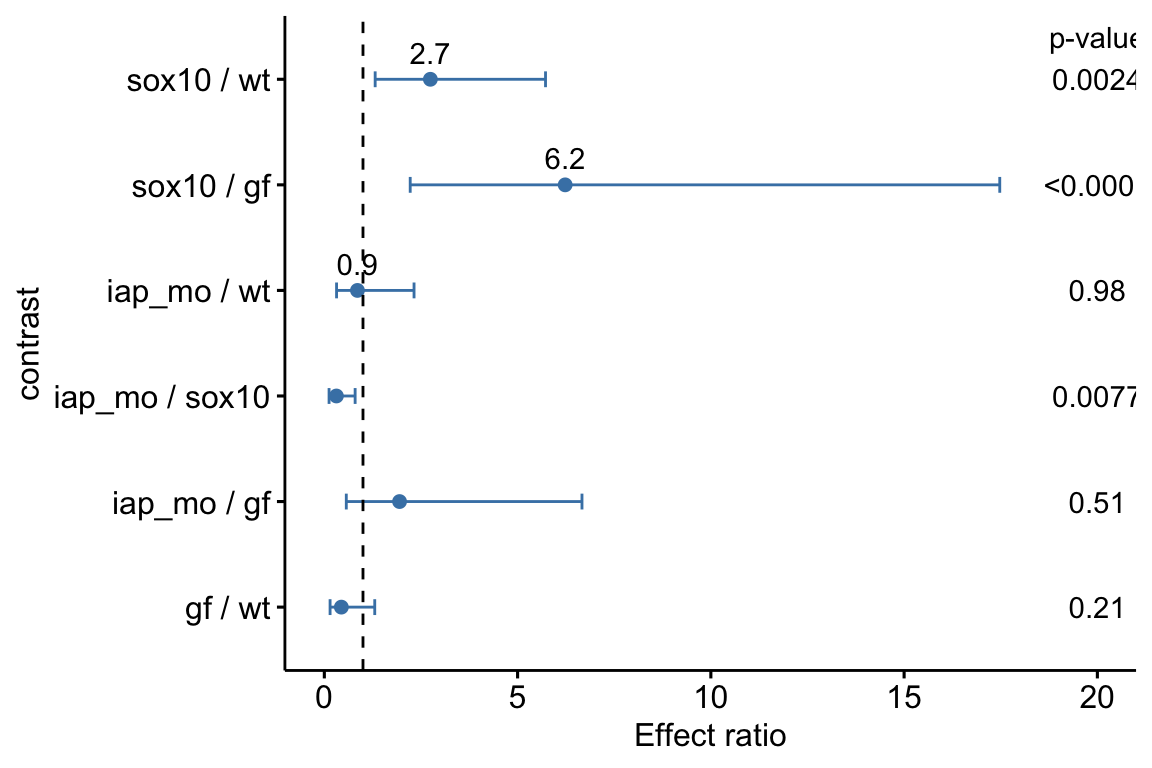
\includegraphics{Walker-elementary-statistical-modeling-draft_files/figure-latex/plots-effect-1.pdf}
\caption{\label{fig:plots-effect}Effects Plot}
\end{figure}

The y-axis contains each of the \emph{paired comparisons} among the four
treatment levels. The x-axis is the response, which is the ratio of the
means of the two groups in the comparison. For example, the top
comparison shows that guts in fish exposed to sox10 donors have 2.7X
more neutrophils per length of gut than guts in fish exposed to wild
type donors. The bars are 95\% confidence intervals, with is the range
of effects that are compatible with the observed data at the 95\% level
(confidence intervals are disscussed in depth in chapter xxx.). The
small end of the interval for the sox10/WT comparison is 1.31, meaning
that effects as small as 31\% increased neutrophil count are compatible
with the data. It is up to the research community to decide if 2.7X or
1.31X are physiologically meaningful effects. \emph{p}-values from the
hypothesis tests are included.

\subsection{Pretty good plot component 2: Modeled mean and CI plot with
jittered raw
data}\label{pretty-good-plot-component-2-modeled-mean-and-ci-plot-with-jittered-raw-data}

Often the means of the treatment levels are meaningful, for example, if
neutrophils per length of gut is a standard measure then researchers
working in this area will be familiar with usual and unusal values. The
data used in Fig \ref{fig:plots-effect} are used to plot means and
confidence intervals of the mean using a \textbf{bar chart}, which is a
pretty good chart type for measures such as counts in which negative
values are prohibited and zero is meaningful.

\begin{figure}
\centering
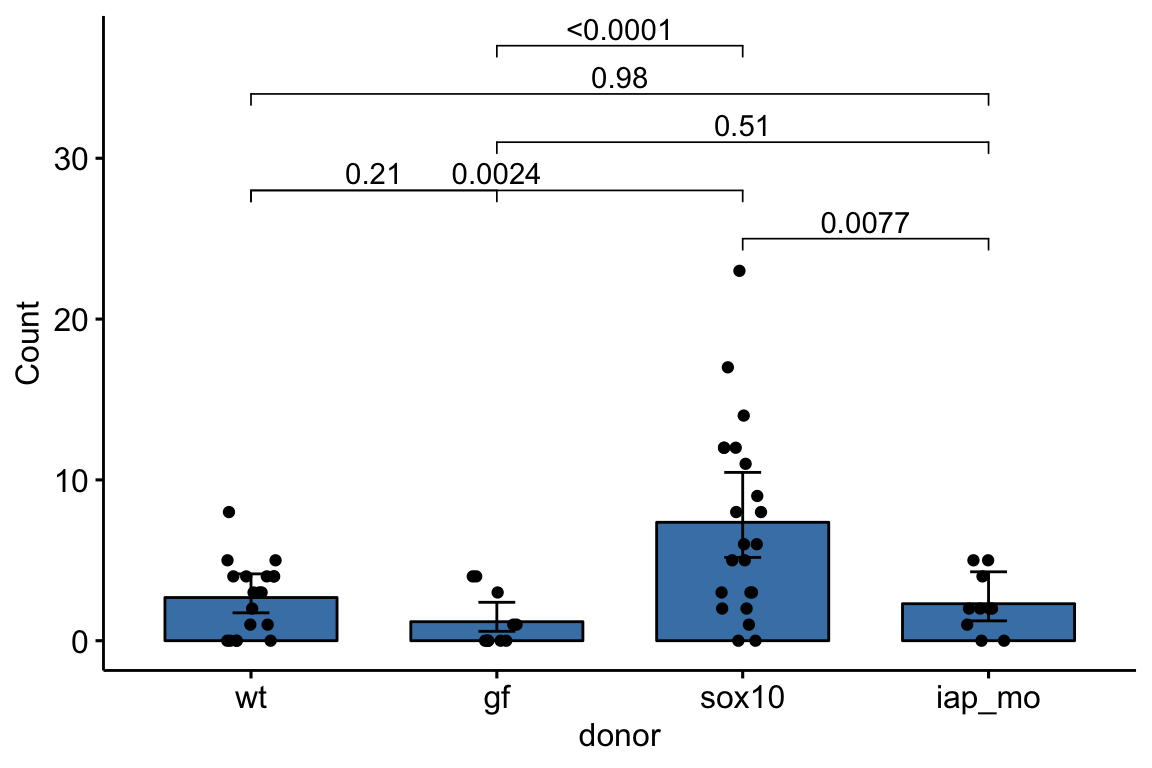
\includegraphics{Walker-elementary-statistical-modeling-draft_files/figure-latex/plots-means-1.pdf}
\caption{\label{fig:plots-means}Mean and error plot}
\end{figure}

Fig. \ref{fig:plots-means} plots the \emph{modeled} means, represented
by the tops of the bars, the modeled 95\% confidence intervals of each
mean, represented by the error bars, and the \emph{p}-values for all
pairwise comparisons. What do I mean by \emph{modeled} means and error
intervals?

\begin{enumerate}
\def\labelenumi{\arabic{enumi}.}
\tightlist
\item
  Modeled means and error intervals are estimated from the statistical
  model. Many published plots are of raw means and error intervals,
  meaning that the mean and error for each treatment level is computed
  only using the response measures in that treatment level.
\item
  A modeled mean will often be equal to the raw mean, but this will not
  always be the case, for example if there are covariates in the model,
  or the researchers are using a \emph{hierarchical model} (Chapter
  xxx).
\item
  Modeled error intervals are never the same as the raw error intervals,
  and are commonly conspicuously different. Almost always, we should
  plot modeled means and error intervals, since these represent the
  means that are relevant to inference.
\end{enumerate}

Fig. \ref{fig:plots-means} also plots the raw count data as ``jittered''
black dots. ``Showing the data'' is a pretty good feature of a plot
because it allows the reader to get a sense of the underlying sample
size and distribution including outliers, which can be used to mentally
model check the published statistical analysis. For example, the
jittered dots in Fig. \ref{fig:plots-means} suggest a
\textbf{heterogeneity} of variances; specifically, the treatment level
with the largest mean has a conspicuously higher variance. This pattern
violates the assumptions of a general linear model and should raise a
red flag to a reader if the researchers used a general linear model to
analyze the data.

What a mean-and-error plot fails to show, at least directly, are the
effects. To infer the effects from the plot, a reader must perform
mental math -- either compute the difference or the ratio between pairs
of means. This mental math is easy enough if the comparisons are between
individual treatment levels but much harder if the comparisons are
between pooled sets of treatment levels, for example in a factorial
experimental design. The mental math that is excessively difficult is
the reconstruction of some kind of error interval of the contrasts, for
example the 95\% confidence intervals in Fig. \ref{plots-effect} and it
is this interval that is necessary for a researcher to infer the range
of biological consequences that are compatible with the experiment. The
inclusion of the \emph{p}-values for all pairwise comparisons gives the
significance level of these contrasts, but of the kinds of summary
results that we could present (contrasts, error intervals,
\emph{p}-values), the \emph{p}-values are the least informative.

\subsection{Combining Effects and Modeled mean and CI plots -- an
Effects and response
plot.}\label{combining-effects-and-modeled-mean-and-ci-plots-an-effects-and-response-plot.}

If one wants to show both effects and the data, then these can be
combined.

\begin{figure}
\centering
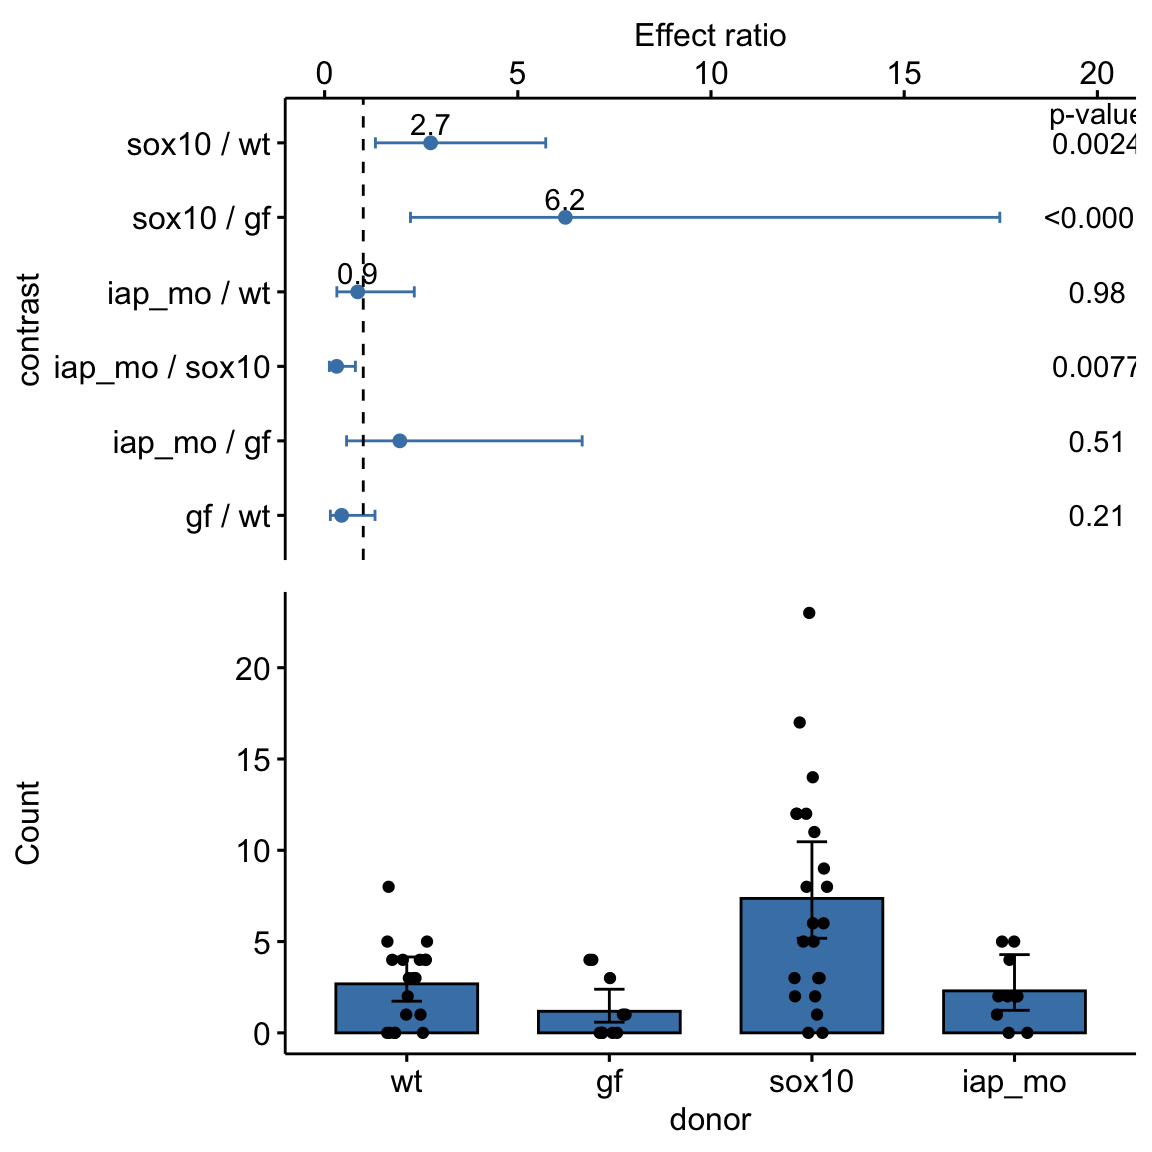
\includegraphics{Walker-elementary-statistical-modeling-draft_files/figure-latex/plots-harrellplot-1.pdf}
\caption{\label{fig:plots-harrellplot}A pretty good plot}
\end{figure}

If the means do not have any importance in understanding the results,
the effects plot can be combined with some kind of a plot summarizing
the distribution, such as a boxplot.

\begin{figure}
\centering
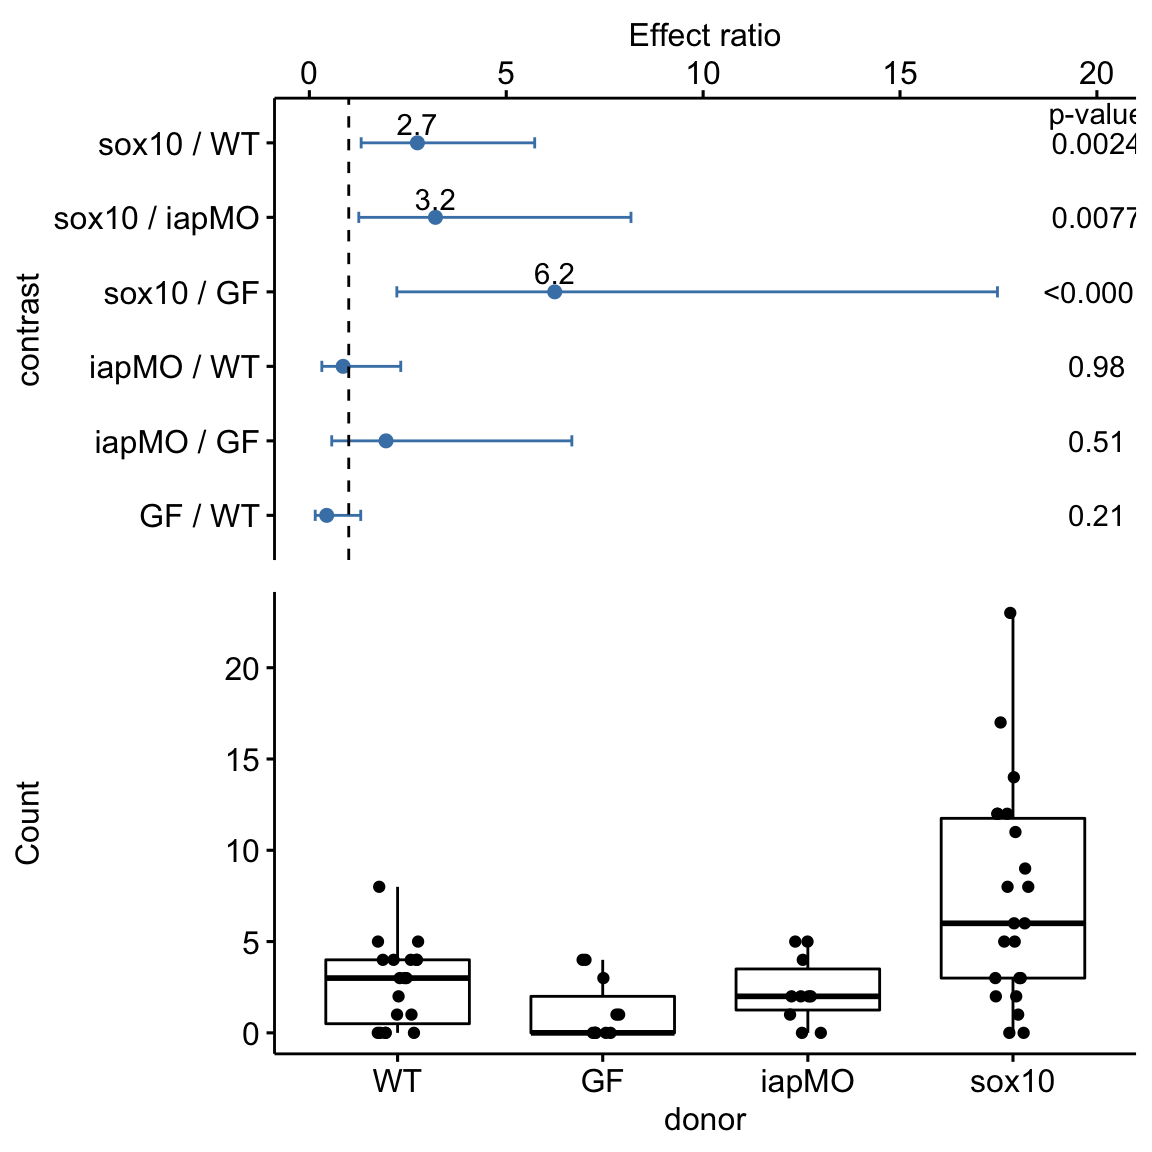
\includegraphics{Walker-elementary-statistical-modeling-draft_files/figure-latex/plots-harrelplot2-1.pdf}
\caption{\label{fig:plots-harrelplot2}Another pretty good plot}
\end{figure}

Regardless, the effects plot is the most important component as this is
the illustration of the story a researcher wants to tell.

\section{Some comments on plot
components}\label{some-comments-on-plot-components}

\begin{enumerate}
\def\labelenumi{\arabic{enumi}.}
\tightlist
\item
  \textbf{Alternatives to barplots make good plots for the supplement,
  not the main paper}. A prominent trend over the last few years has
  been the replacement of bar plots with plots that ``show the data'',
  such as jitter plots or dot plots, or that show summaries of the
  distribution, such as box plots or violin plots. These plot types were
  developed for exploratory data analysis, not to communicate the
  results of experiments. All of these plots fail to communicate the
  results of the statistical model and, because of this, are inferior to
  an effects plot, and even a mean-and-error plot, if the mean and error
  are the modeled values. Box/Violoin/Dot/Jitter plots are a useful
  supplement to an effects plot, either combined with the effects plot
  as above, or as a supplementary figure.
\item
  Standard error bars, computed from the raw data, can have absurd
  implications. For example, I sometimes see standard error bars cross
  \(y=0\) for a response that cannot be negative, such as a count. Even
  if the standard error bar doesn't cross zero, it is common to see
  standard error bars that imply (but do not explicitly show) 95\%
  confidence intervals that cross zero, again for responses that cannot
  be negative. A standard error bar or confidence interval that crosses
  zero implies that negative means are compatible with the data. This is
  an absurd implication for responses that cannot have negative values
  (or are ``bounded by'' zero). Explicit or implicit error bars that
  cross zero are especially common for count responses with small means.
  \emph{If} a researcher plots confidence intervals, these should be
  computed using a method that avoids absurd implications, such methods
  include the bootstrap and generalized linear models.
\item
  \textbf{Stars add minimal value}. Many researchers add star symbols to
  a plot indicating the level of significance of a particular paired
  comparison. An uncommon, but better, alternative would be to add the
  actual p-value (as above). Adding a p-value (or stars) does
  communicate model results, and so adds value to a mean-and-error or
  box/violin/jitter plot. However, much more value would be added by
  simply reporting an effects plot or a combined effects-and-response
  plot.
\end{enumerate}

\section{Working in R}\label{working-in-r-2}

A reasonable goal of any research project should be a script to generate
the final plots entirely within the R environment and not rely on
external drawing software to add finishing features. \texttt{ggplot2} is
one of the major plotting environments in R and the one that seems to
have the strongest following, especially among new R users.
\texttt{ggplot2} has the ability to generate extremely personalized and
finished plots. However, creating a plot with multiple layers (bars,
lines, error intervals, raw data points, p-values) can often require
many hours of googling.

\texttt{ggpubr} is an extension to \texttt{ggplot2} (it calls ggplot2
functions under the hood) and provides many canned functions for
producing the kinds of ggplots that are published in biological
journals. With one line of script, a researcher can generate a
publishable plot that is as good or better than many published plot.
That said, the means and error intervals used in \texttt{ggpubr} plots
are the raw and not modeled values, and, consequently, \texttt{ggpubr}
is not sufficient to generate pretty good plots. It is easy enough to
add custom error bars to a ggpubr plot.

\subsection{Adding modeled error
intervals}\label{adding-modeled-error-intervals}

\texttt{ggplot2} and \texttt{ggpubr} compute and plot unpooled error
intervals (standard error bars and confidence intervals). Plotting the
modeled error intervals ``shows the model''. \texttt{emmeans} is a
comprehensive and flexible package for computing modeled standard errors
and confidence intervals for all of the statistical models covered in
this text.

\begin{Shaded}
\begin{Highlighting}[]
\NormalTok{m1 <-}\StringTok{ }\KeywordTok{glm.nb}\NormalTok{(count }\OperatorTok{~}\StringTok{ }\NormalTok{donor, }\DataTypeTok{data=}\NormalTok{exp2d)}
\NormalTok{emm.m1 <-}\StringTok{ }\KeywordTok{emmeans}\NormalTok{(m1, }\DataTypeTok{specs=}\StringTok{"donor"}\NormalTok{, }\DataTypeTok{type=}\StringTok{"response"}\NormalTok{)}
\NormalTok{effects.m1 <-}\StringTok{ }\KeywordTok{summary}\NormalTok{(}\KeywordTok{contrast}\NormalTok{(emm.m1, }\DataTypeTok{method=}\StringTok{"revpairwise"}\NormalTok{), }\DataTypeTok{infer=}\KeywordTok{c}\NormalTok{(}\OtherTok{TRUE}\NormalTok{, }\OtherTok{TRUE}\NormalTok{))}

\CommentTok{# make emm.m1 a data.table}
\NormalTok{emm.m1 <-}\StringTok{ }\KeywordTok{data.table}\NormalTok{(}\KeywordTok{summary}\NormalTok{(emm.m1))}
\CommentTok{# the y column needs to have the same label as the plotted data}
\KeywordTok{setnames}\NormalTok{(emm.m1, }\DataTypeTok{old=}\StringTok{"response"}\NormalTok{, }\DataTypeTok{new=}\StringTok{"count"}\NormalTok{)}
\end{Highlighting}
\end{Shaded}

\subsubsection{Modeled error intervals of the
effect}\label{modeled-error-intervals-of-the-effect}

\begin{Shaded}
\begin{Highlighting}[]
\NormalTok{(gg1 <-}\StringTok{ }\KeywordTok{ggdotplot}\NormalTok{(}\DataTypeTok{x=}\StringTok{"contrast"}\NormalTok{, }
                 \DataTypeTok{y=}\StringTok{"ratio"}\NormalTok{, }
                 \DataTypeTok{data=}\NormalTok{effects.m1, }
                 \DataTypeTok{color =} \StringTok{"steelblue"}\NormalTok{,}
                 \DataTypeTok{fill =} \StringTok{"steelblue"}\NormalTok{,}
                 \DataTypeTok{size=}\FloatTok{0.5}\NormalTok{) }\OperatorTok{+}
\StringTok{   }
\StringTok{  }\CommentTok{# add either the SE or CI, contained in effects.m1}
\StringTok{  }\KeywordTok{geom_errorbar}\NormalTok{(}\KeywordTok{aes}\NormalTok{(}\DataTypeTok{x=}\NormalTok{contrast, }\DataTypeTok{ymin=}\NormalTok{asymp.LCL, }\DataTypeTok{ymax=}\NormalTok{asymp.UCL),}
                \DataTypeTok{width=}\FloatTok{0.15}\NormalTok{, }\DataTypeTok{color=}\StringTok{"steelblue"}\NormalTok{) }\OperatorTok{+}
\StringTok{  }\KeywordTok{ylab}\NormalTok{(}\StringTok{"Effect ratio"}\NormalTok{) }\OperatorTok{+}
\StringTok{  }\KeywordTok{geom_hline}\NormalTok{(}\DataTypeTok{yintercept=}\DecValTok{1}\NormalTok{, }\DataTypeTok{linetype =} \DecValTok{2}\NormalTok{) }\OperatorTok{+}
\StringTok{  }\KeywordTok{coord_flip}\NormalTok{() }\OperatorTok{+}\StringTok{ }
\StringTok{  }
\StringTok{  }\OtherTok{NULL}\NormalTok{)}
\end{Highlighting}
\end{Shaded}

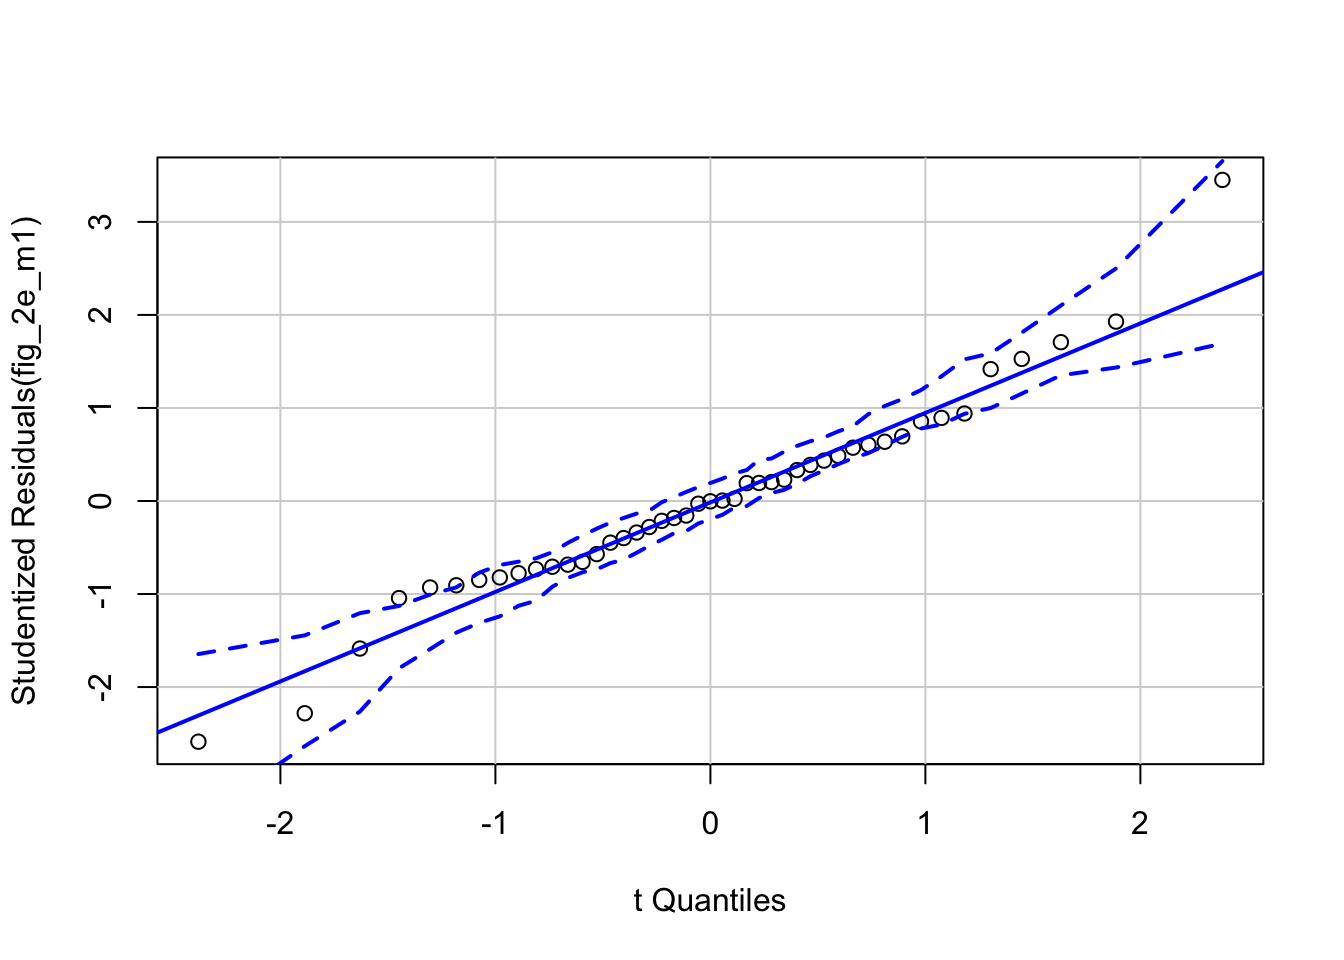
\includegraphics{Walker-elementary-statistical-modeling-draft_files/figure-latex/unnamed-chunk-24-1.pdf}

\subsubsection{Modeled error intervals of the
mean}\label{modeled-error-intervals-of-the-mean}

\begin{Shaded}
\begin{Highlighting}[]
\NormalTok{(gg2 <-}\StringTok{ }\KeywordTok{ggbarplot}\NormalTok{(}\DataTypeTok{x=}\StringTok{"donor"}\NormalTok{, }
          \DataTypeTok{y=}\StringTok{"count"}\NormalTok{, }
          \DataTypeTok{data=}\NormalTok{exp2d,}
          \DataTypeTok{add=}\KeywordTok{c}\NormalTok{(}\StringTok{"mean"}\NormalTok{, }\StringTok{"jitter"}\NormalTok{),}
          \DataTypeTok{color =} \StringTok{"darkgray"}\NormalTok{,}
          \DataTypeTok{fill =} \StringTok{"steelblue"}\NormalTok{,}
          \DataTypeTok{size=}\FloatTok{0.5}\NormalTok{) }\OperatorTok{+}
\StringTok{  }\KeywordTok{ylab}\NormalTok{(}\StringTok{"Neutrophil count"}\NormalTok{) }\OperatorTok{+}
\StringTok{  }
\StringTok{  }\CommentTok{# emm.m1 contains the SE and 95% CIs. Either could be plotted. Here I plot the CI}
\StringTok{  }\KeywordTok{geom_errorbar}\NormalTok{(}\DataTypeTok{data=}\NormalTok{emm.m1, }\KeywordTok{aes}\NormalTok{(}\DataTypeTok{ymin=}\NormalTok{asymp.LCL, }\DataTypeTok{ymax=}\NormalTok{asymp.UCL), }\DataTypeTok{width=}\FloatTok{0.1}\NormalTok{) }\OperatorTok{+}
\StringTok{  }\OtherTok{NULL}\NormalTok{)}
\end{Highlighting}
\end{Shaded}

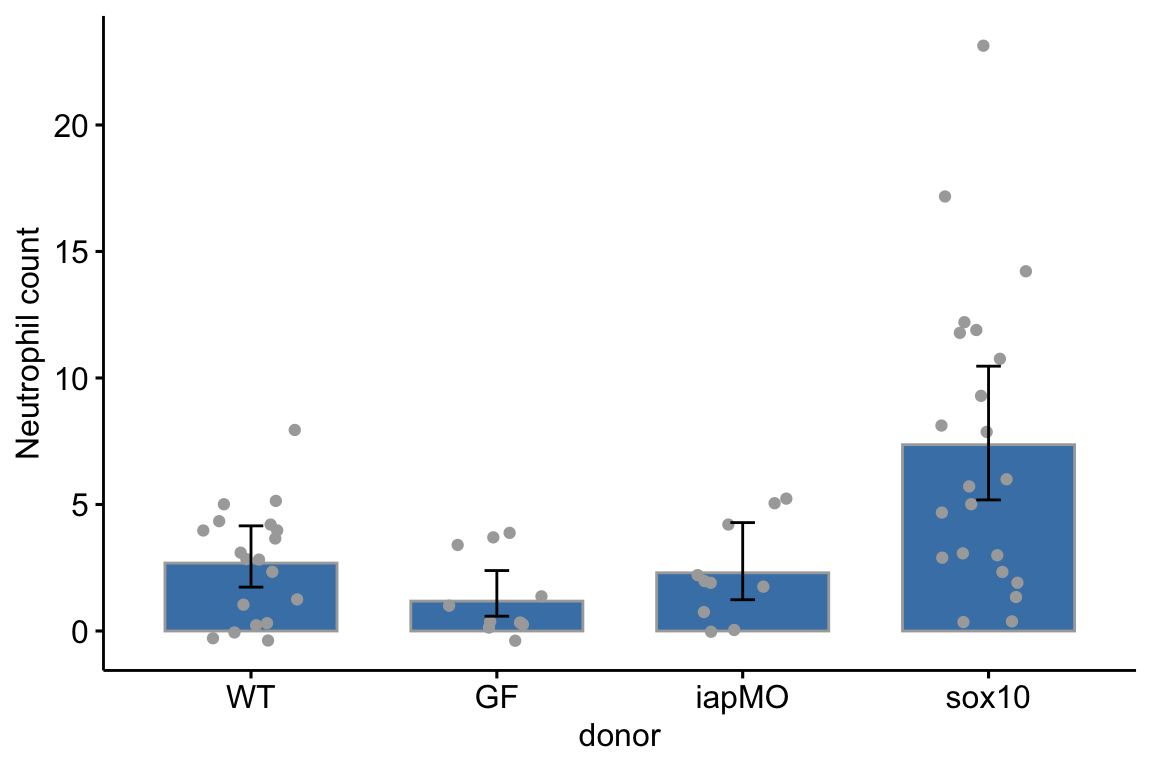
\includegraphics{Walker-elementary-statistical-modeling-draft_files/figure-latex/unnamed-chunk-25-1.pdf}

Note that the CIs are asymmetric about the mean (and these modeled CIs
will never include negative values for count data).

\subsubsection{Combining effects and response
plots}\label{combining-effects-and-response-plots}

The ggplots are combined using the package \texttt{cowplot}

\begin{Shaded}
\begin{Highlighting}[]
\NormalTok{gg_top <-}\StringTok{ }\NormalTok{gg1 }\OperatorTok{+}\StringTok{ }\KeywordTok{scale_y_continuous}\NormalTok{(}\DataTypeTok{position=}\StringTok{"right"}\NormalTok{)}
\KeywordTok{plot_grid}\NormalTok{(gg_top, gg2, }\DataTypeTok{nrow=}\DecValTok{2}\NormalTok{, }\DataTypeTok{align =} \StringTok{"v"}\NormalTok{, }\DataTypeTok{rel_heights =} \KeywordTok{c}\NormalTok{(}\DecValTok{1}\NormalTok{, }\DecValTok{1}\NormalTok{))}
\end{Highlighting}
\end{Shaded}

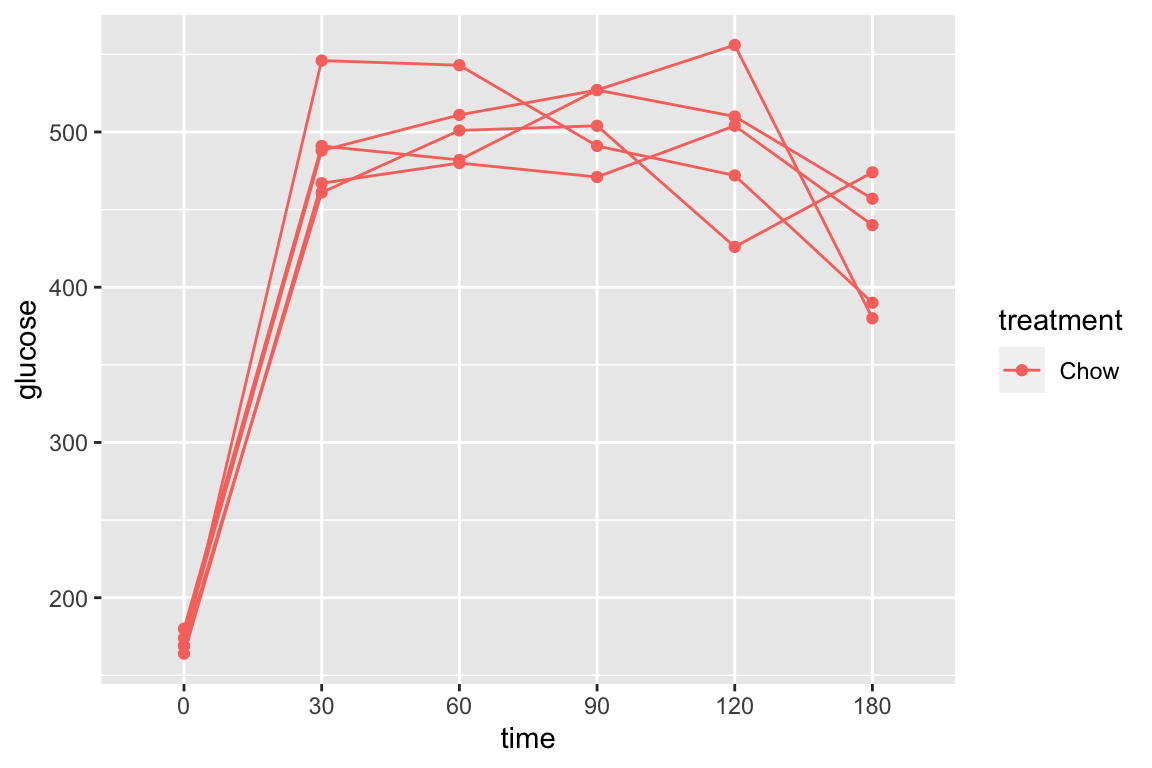
\includegraphics{Walker-elementary-statistical-modeling-draft_files/figure-latex/unnamed-chunk-26-1.pdf}

\subsection{Adding p-values}\label{adding-p-values}

p-values are added to the base ggpubr plot using
\texttt{stat\_compare\_means}. The pairs to compare are specified with
\texttt{comparison\ =}. The model to compute the p-values is ``t.test''.
\textbf{It is important to know what exactly is being computed when
analyzing data and reporting results} and ``t test'' is not sufficient
to know this. The t-test could be the classic t-test or a Welch test
(which adjusts the standard error to account for heterogenity in
variance between groups). In this example, there are multiple tests and
the standard error could be the pooled estimate estimated from the
linear model, or a pairwise estimate. And, given the multiple
comparisons, the p-values could be adjusted or not. These kinds of
questions can be checked with a function's help page.
\texttt{?stat\_compare\_means} doesn't answer these questions but
suggests \texttt{compare\_means}, which also doesn't answer these
questions. The script below has checks to see what p-values the function
is returning.

\begin{Shaded}
\begin{Highlighting}[]
\NormalTok{pairs_i <-}\StringTok{ }\KeywordTok{list}\NormalTok{(}\KeywordTok{c}\NormalTok{(}\StringTok{"sox10"}\NormalTok{, }\StringTok{"iapMO"}\NormalTok{), }\KeywordTok{c}\NormalTok{(}\StringTok{"sox10"}\NormalTok{, }\StringTok{"GF"}\NormalTok{), }\KeywordTok{c}\NormalTok{(}\StringTok{"sox10"}\NormalTok{, }\StringTok{"WT"}\NormalTok{))}
\KeywordTok{ggbarplot}\NormalTok{(}\DataTypeTok{x=}\StringTok{"donor"}\NormalTok{, }
          \DataTypeTok{y=}\StringTok{"count"}\NormalTok{, }
          \DataTypeTok{data=}\NormalTok{exp2d,}
          \DataTypeTok{add=}\KeywordTok{c}\NormalTok{(}\StringTok{"mean_se"}\NormalTok{, }\StringTok{"jitter"}\NormalTok{),}
          \DataTypeTok{color =} \StringTok{"black"}\NormalTok{,}
          \DataTypeTok{fill =} \StringTok{"steelblue"}\NormalTok{,}
          \DataTypeTok{size=}\FloatTok{0.5}\NormalTok{) }\OperatorTok{+}
\StringTok{  }\KeywordTok{stat_compare_means}\NormalTok{(}\DataTypeTok{method =} \StringTok{"t.test"}\NormalTok{, }\DataTypeTok{comparisons=}\NormalTok{pairs_i) }\OperatorTok{+}
\StringTok{  }\KeywordTok{ylab}\NormalTok{(}\StringTok{"Neutrophil count"}\NormalTok{) }\OperatorTok{+}
\StringTok{  }\OtherTok{NULL}
\end{Highlighting}
\end{Shaded}

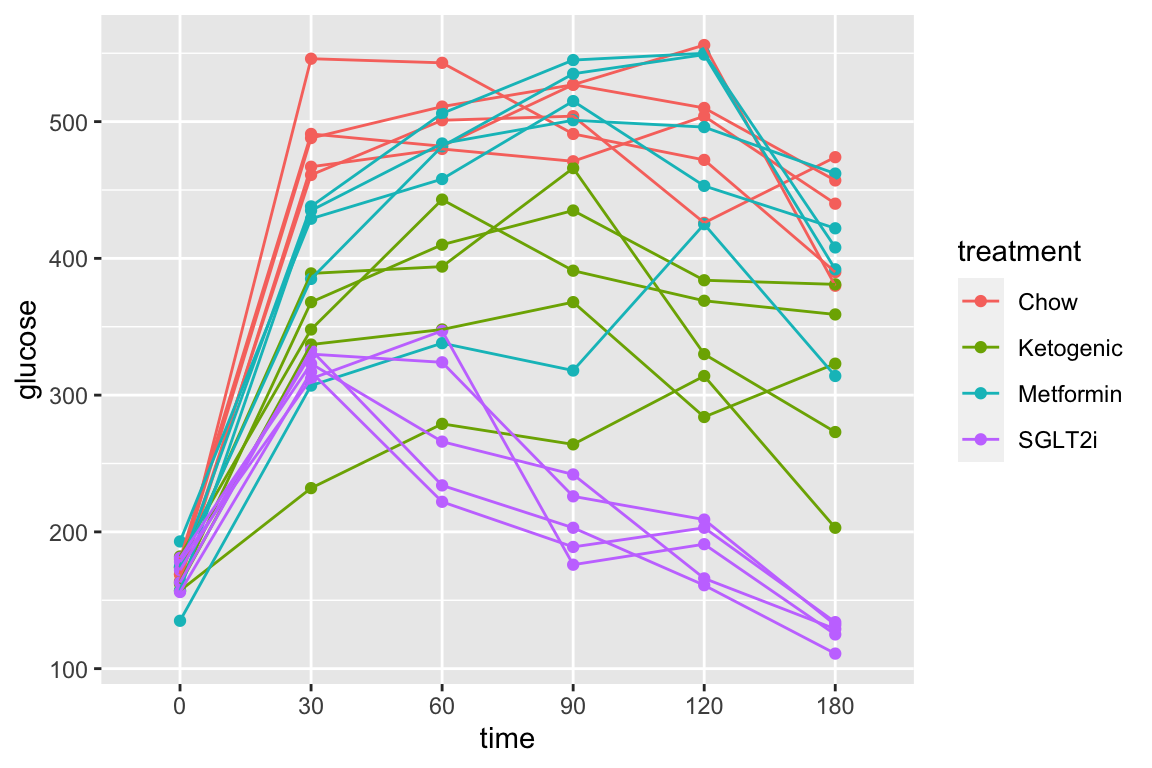
\includegraphics{Walker-elementary-statistical-modeling-draft_files/figure-latex/unnamed-chunk-27-1.pdf}

\begin{Shaded}
\begin{Highlighting}[]
\CommentTok{# checks on the p-value}
\CommentTok{# t-tests using SE pooled over all four groups}
\NormalTok{check_it <-}\StringTok{ }\OtherTok{FALSE}
\ControlFlowTok{if}\NormalTok{(check_it}\OperatorTok{==}\OtherTok{TRUE}\NormalTok{)\{}
\NormalTok{  m1 <-}\StringTok{ }\KeywordTok{lm}\NormalTok{(count}\OperatorTok{~}\NormalTok{donor, }\DataTypeTok{data=}\NormalTok{exp2d)}
\NormalTok{  m1.emm <-}\StringTok{ }\KeywordTok{emmeans}\NormalTok{(m1, }\DataTypeTok{specs=}\StringTok{"donor"}\NormalTok{)}
  \KeywordTok{contrast}\NormalTok{(m1.emm, }\DataTypeTok{method=}\StringTok{"trt.vs.ctrl"}\NormalTok{, }\DataTypeTok{ref=}\DecValTok{3}\NormalTok{, }\DataTypeTok{adjust=}\StringTok{"none"}\NormalTok{) }\CommentTok{# not pooled SE}
  
  \KeywordTok{pairwise.t.test}\NormalTok{(exp2d}\OperatorTok{$}\NormalTok{count, exp2d}\OperatorTok{$}\NormalTok{donor, }\DataTypeTok{p.adjust.method=}\StringTok{"none"}\NormalTok{, }\DataTypeTok{pool.sd=}\OtherTok{FALSE}\NormalTok{) }\CommentTok{# this matches}
  \CommentTok{# compare}
  \KeywordTok{t.test}\NormalTok{(count}\OperatorTok{~}\NormalTok{donor, }\DataTypeTok{data=}\NormalTok{exp2d[donor}\OperatorTok{==}\StringTok{"WT"} \OperatorTok{|}\StringTok{ }\NormalTok{donor}\OperatorTok{==}\StringTok{"sox10"}\NormalTok{]) }\CommentTok{# matches, this is Welch t}
  \KeywordTok{t.test}\NormalTok{(count}\OperatorTok{~}\NormalTok{donor, }\DataTypeTok{data=}\NormalTok{exp2d[donor}\OperatorTok{==}\StringTok{"WT"} \OperatorTok{|}\StringTok{ }\NormalTok{donor}\OperatorTok{==}\StringTok{"sox10"}\NormalTok{], }\DataTypeTok{var.equal=}\OtherTok{TRUE}\NormalTok{)}
\NormalTok{\}}
\end{Highlighting}
\end{Shaded}

So the p-values returned by
\texttt{stat\_compare\_means(method="t.test")} are computed from
independent Welch t-tests.

\subsection{Adding custom p-values}\label{adding-custom-p-values}

\subsection{Plotting two factors}\label{plotting-two-factors}

The data are from figure 6d. This solution requires computing either the
raw or modeled means and errors and adding these to a base ggpubr plot.
Many packages have summary statistics functions for means, standard
deviations, and standard errors. This is easily done by simply computing
the statistics using data.table functionality.

\begin{Shaded}
\begin{Highlighting}[]
\CommentTok{# compute raw statistics}
\CommentTok{# enclosing the line within parentheses prints the result to the console!}
\NormalTok{(exp6d.raw <-}\StringTok{ }\NormalTok{exp6d[}\OperatorTok{!}\KeywordTok{is.na}\NormalTok{(count), .(}\DataTypeTok{count=}\KeywordTok{mean}\NormalTok{(count),}
                       \DataTypeTok{se=}\KeywordTok{sd}\NormalTok{(count)}\OperatorTok{/}\KeywordTok{sqrt}\NormalTok{(.N)),}
                   \DataTypeTok{by=}\NormalTok{.(treatment, strain)]}
\NormalTok{)}
\end{Highlighting}
\end{Shaded}

\begin{verbatim}
##     treatment strain    count       se
## 1:    control     WT 13.08333 2.310904
## 2:    control  sox10 45.61538 6.259903
## 3: transplant     WT 16.35714 2.259552
## 4: transplant  sox10 18.33333 4.536274
\end{verbatim}

Modeled means, standard errors, and confidence limits are conveniently
computed using the \texttt{emmeans} (``estimated marginal means'')
function from the emmeans package.

\begin{Shaded}
\begin{Highlighting}[]
\CommentTok{# modeled statsistics}
\NormalTok{m1 <-}\StringTok{ }\KeywordTok{glm.nb}\NormalTok{(count }\OperatorTok{~}\StringTok{ }\NormalTok{treatment}\OperatorTok{*}\NormalTok{strain, }\DataTypeTok{data=}\NormalTok{exp6d)}
\NormalTok{(m1.emm <-}\StringTok{ }\KeywordTok{data.table}\NormalTok{(}\KeywordTok{summary}\NormalTok{(}\KeywordTok{emmeans}\NormalTok{(m1, }\DataTypeTok{specs=}\KeywordTok{c}\NormalTok{(}\StringTok{"treatment"}\NormalTok{, }\StringTok{"strain"}\NormalTok{), }\DataTypeTok{type=}\StringTok{"response"}\NormalTok{))))}
\end{Highlighting}
\end{Shaded}

\begin{verbatim}
##     treatment strain response       SE  df asymp.LCL asymp.UCL
## 1:    control     WT 13.08333 2.032161 Inf  9.649528  17.73907
## 2: transplant     WT 16.35714 2.289208 Inf 12.433129  21.51961
## 3:    control  sox10 45.61538 6.132974 Inf 35.048350  59.36837
## 4: transplant  sox10 18.33333 3.871911 Inf 12.119140  27.73391
\end{verbatim}

\begin{Shaded}
\begin{Highlighting}[]
\CommentTok{# change column "response" to "count" for the ggplot}
\KeywordTok{setnames}\NormalTok{(m1.emm, }\DataTypeTok{old=}\StringTok{"response"}\NormalTok{, }\DataTypeTok{new=}\StringTok{"count"}\NormalTok{)}
\end{Highlighting}
\end{Shaded}

\begin{Shaded}
\begin{Highlighting}[]
\CommentTok{#pairs_i <- list(c("sox10", "iapMO"), c("sox10", "GF"), c("sox10", "WT"))}
\NormalTok{pd =}\StringTok{ }\KeywordTok{position_dodge}\NormalTok{(}\FloatTok{0.7}\NormalTok{)}
\KeywordTok{ggbarplot}\NormalTok{(}\DataTypeTok{x=}\StringTok{"treatment"}\NormalTok{, }
          \DataTypeTok{y=}\StringTok{"count"}\NormalTok{,}
          \DataTypeTok{data=}\NormalTok{exp6d,}
          \DataTypeTok{add=}\KeywordTok{c}\NormalTok{(}\StringTok{"mean"}\NormalTok{),}
          \DataTypeTok{color =} \StringTok{"black"}\NormalTok{,}
          \DataTypeTok{fill =} \StringTok{"strain"}\NormalTok{,}
          \DataTypeTok{palette =} \StringTok{"jco"}\NormalTok{,}
          \DataTypeTok{position =}\NormalTok{ pd,}
          \DataTypeTok{size=}\FloatTok{0.5}\NormalTok{) }\OperatorTok{+}
\StringTok{  }\CommentTok{#stat_compare_means(method = "t.test", comparisons=pairs_i) +}
\StringTok{  }\KeywordTok{ylab}\NormalTok{(}\StringTok{"Neutrophil count"}\NormalTok{) }\OperatorTok{+}
\StringTok{  }\CommentTok{# geom_dotplot(aes(fill=strain),}
\StringTok{  }\CommentTok{#              binaxis='y', stackdir='center', position=pd, show.legend=FALSE,}
\StringTok{  }\CommentTok{#              color="grey") +}
\StringTok{  }\KeywordTok{geom_point}\NormalTok{(}\KeywordTok{aes}\NormalTok{(}\DataTypeTok{fill=}\NormalTok{strain), }\DataTypeTok{position=}\KeywordTok{position_jitterdodge}\NormalTok{(}\DataTypeTok{jitter.width=}\FloatTok{0.2}\NormalTok{), }\DataTypeTok{show.legend=}\OtherTok{FALSE}\NormalTok{, }\DataTypeTok{alpha=}\FloatTok{0.5}\NormalTok{) }\OperatorTok{+}
\StringTok{  }\KeywordTok{geom_errorbar}\NormalTok{(}\DataTypeTok{data=}\NormalTok{m1.emm, }\KeywordTok{aes}\NormalTok{(}\DataTypeTok{x=}\NormalTok{treatment, }\DataTypeTok{ymin=}\NormalTok{asymp.LCL, }\DataTypeTok{ymax=}\NormalTok{asymp.UCL, }\DataTypeTok{group=}\NormalTok{strain),}
                \DataTypeTok{position=}\NormalTok{pd, }\DataTypeTok{width=}\FloatTok{0.1}\NormalTok{) }\OperatorTok{+}
\StringTok{  }\OtherTok{NULL}
\end{Highlighting}
\end{Shaded}

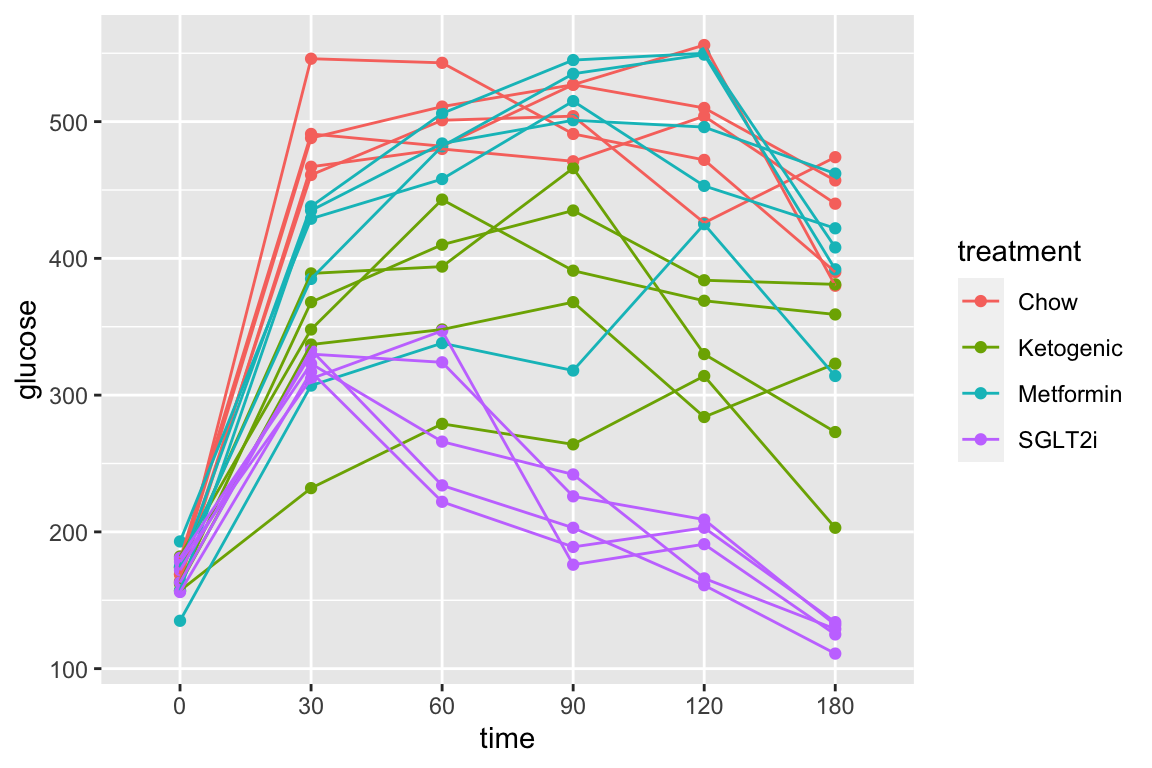
\includegraphics{Walker-elementary-statistical-modeling-draft_files/figure-latex/unnamed-chunk-30-1.pdf}

\subsubsection{Three factors}\label{three-factors}

\chapter*{\texorpdfstring{Part IV: More than one \(X\) -- Multivariable
Models}{Part IV: More than one X -- Multivariable Models}}\label{part-iv-more-than-one-x-multivariable-models}
\addcontentsline{toc}{chapter}{Part IV: More than one \(X\) --
Multivariable Models}

\chapter{Adding covariates to a linear
model}\label{adding-covariates-to-a-linear-model}

In its most general sense, \textbf{Covariates} are simply the \(X\)
variables in a statistical model. With data from experiments,
``covariates'' more typically refers to \(X\) variables that are added
to a model to increase precision of the treatment effects. In
observational designs, covariates might be added to a model to 1)
increase predictive ability, 2) because the researcher is interested in
specific conditional effects, or 3) to eliminate confounding. These are
discussed in later chapters.

\section{Adding covariates can increases the precision of the effect of
interest}\label{adding-covariates-can-increases-the-precision-of-the-effect-of-interest}

I use fake data to introduce the concept of \textbf{statistical
elimination} of a \textbf{covariate} in a statistical model. Here I am
modeling the effect of a new drug on blood LDL-C levels. LDL is a kind
of lipoprotein, which are particles in the blood that transport fats and
cholesterol to and from different tissues. LDL-C is cholesterol
associated with LDL particles. LDL-C is considered ``bad cholesterol''
because LDL is believed to transport cholesterol and other lipids to
arterial walls, which is the basis for atherosclerosis.

Twenty applied biostats students are recruited and are randomly assigned
to either the new or old drug. The response is blood LDL-C level and the
two treatment levels are ``old'' and ``new''. For the dummy variable
coding, I'll make ``old'' the reference level.

Let's model this with

\begin{equation}
ldlc = \beta_0 + \beta_1 drug + \varepsilon
\label{eq:ancova-1}
\end{equation}

where \(drug\) is the dummy variable with \(old=0\) and \(new=1\).

\begin{figure}
\centering
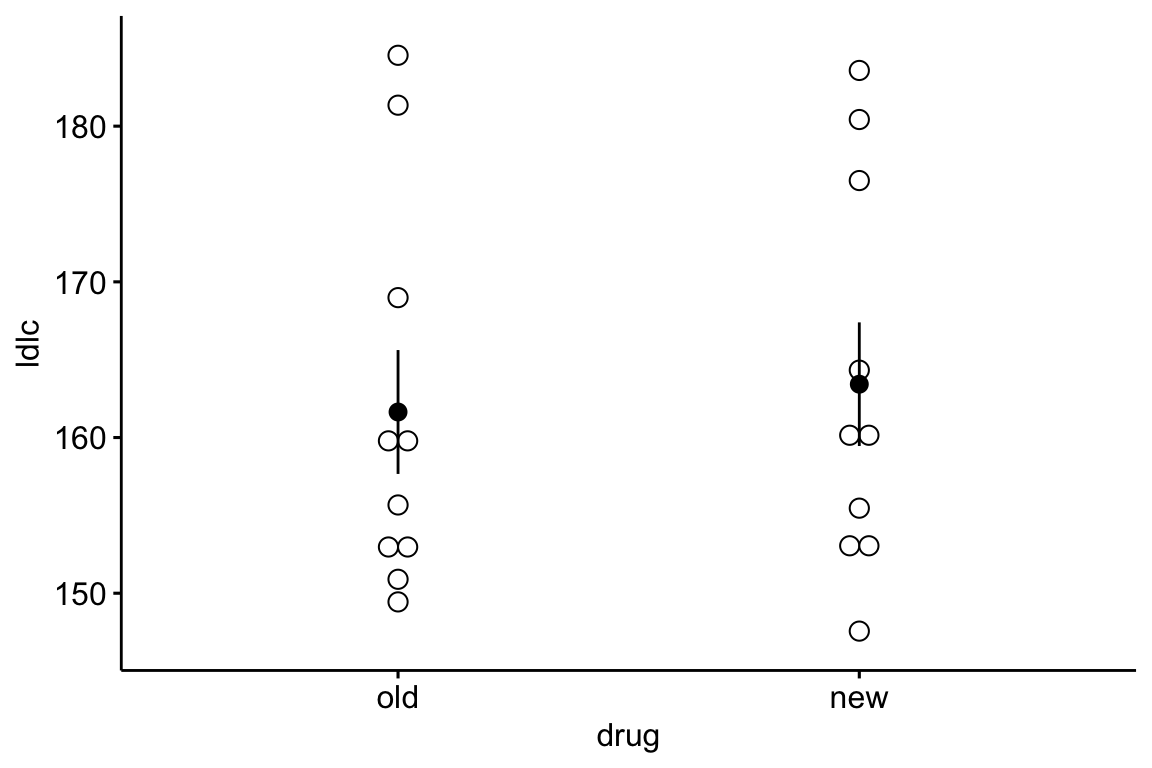
\includegraphics{Walker-elementary-statistical-modeling-draft_files/figure-latex/ancova-plot1-1.pdf}
\caption{\label{fig:ancova-plot1}The fake LDL-C experiment.}
\end{figure}

\begin{verbatim}
##               Estimate Std. Error    t value     Pr(>|t|)
## (Intercept) 161.640772   3.974506 40.6694043 3.620049e-19
## drugnew       1.785414   5.620800  0.3176442 7.544101e-01
\end{verbatim}

The plot shows large overlap in LDL-C and no obvious effect of the drug.
There ``is no effect of the drug (\(p = 0.754\))'' is of course an
incorrect interpretation of the hypothesis test of the estimate of
\(\beta_1\). A correct interpretation is, there is too much noise to say
much about any effect.

In addition to assigning treatment level randomly, I also had the 20
students count calories from fat over the course of the experiment. Here
is a plot of LDL-C vs.~percent calories from fat, with treatment
assignment color coded. Remember, these are the exact same values of
LDL-C as in the first figure.

\begin{figure}
\centering
\includegraphics{Walker-elementary-statistical-modeling-draft_files/figure-latex/ancova-plot2-1.pdf}
\caption{\label{fig:ancova-plot2}Linear regression of \(ldlc\) on dietary
\(fat\) fit to the fake LDL-C data. The points are color coded by
treatment.}
\end{figure}

The line is the bivariate regression fit to the data ignoring treatment
level so is the model

\begin{equation}
ldlc = \beta_0 + \beta_1 fat + \varepsilon
\label{eq:ancova-2}
\end{equation}

I've color coded the points by treatment level but \(drug\) is not in
the model. It is clear that most of the ``old'' data points are above
the line, or have positive residuals from the model, while the ``new''
data points are below the line, or have negative residuals from the
model. A better way to think about this pattern is that \textbf{at any
specific level of fat, the LDL-C for old is higher than the LDL-C for
new}.

What is happening? Dietary fat is contributing to the variance of LDL-C
and this added noise makes it harder to measure the effect of the new
drug relative to the old drug. If we could somehow measure the effect of
drug at a specific level of dietary fat, then we could get a more
precise estimate of the effect. But how to do this?

\begin{enumerate}
\def\labelenumi{\arabic{enumi}.}
\item
  We could just analyze a subset of the data, that is, only the cases in
  which the value of dietary fat is nearly equal. This throws away
  perfectly good data and, consequently, greatly reduces the sample size
  and thus precision to estimate the effect.
\item
  We could use the residuals of the fitted model \eqref{eq:ancova-2} to
  estimate the effect of drug treatment (this is what we did by eye in
  figure \ref{fig:ancova-plot2}). Here is the new model
\end{enumerate}

\begin{equation}
ldlc.r = \beta_0 + \beta_1 drug + \varepsilon
\label{eq:ancova-3}
\end{equation}

where \(ldlc.r\) are the residuals. The effect of the new drug on these
residuals is

\begin{verbatim}
## `stat_bindot()` using `bins = 30`. Pick better value with `binwidth`.
\end{verbatim}

\includegraphics{Walker-elementary-statistical-modeling-draft_files/figure-latex/unnamed-chunk-31-1.pdf}

\begin{verbatim}
##              Estimate Std. Error   t value     Pr(>|t|)
## (Intercept)  2.361321  0.6190269  3.814570 1.269495e-03
## drugnew     -4.722642  0.8754362 -5.394616 3.984159e-05
\end{verbatim}

In this two-stage analysis (stage 1: fit ldlc \textasciitilde{} fat to
get residuals, stage 2: fit residuals \textasciitilde{} drug), we have
\emph{eliminated the effect of dietary fat} on the variance of the
response and, as a consequence, the estimate of the effect of the drug
is much more precise. Now the estimate of the effect is -4.7 mg/dL blood
and the SE is only .9 (compare this to the values in the original
analysis). While the SE of the diference is correct, any confidence
interval or \(t\)-value is not because the df is wrong. In the two stage
analysis we fit two parameters -- the slope (coefficient \(b_1\)) in
stage 1 and the difference in means (coefficient \(b_1\)) in stage 2 --
but the \(t\) in the table assumes we only fit one parameter (that from
stage 2). Effectively, the stage 2 test is ignorant that the data
(\(ldlc.r\)) are the result of a previous model fit. We could manually
modify the computation of \(t\), but the more proper method is to
simply\ldots{}

\begin{enumerate}
\def\labelenumi{\arabic{enumi}.}
\setcounter{enumi}{2}
\tightlist
\item
  Add dietary fat into the original linear model.
\end{enumerate}

\begin{equation}
ldlc = \beta_0 + \beta_1 fat + \beta_2 drug + \varepsilon
\end{equation}

\begin{verbatim}
##               Estimate Std. Error  t value     Pr(>|t|)
## (Intercept)  99.449257  2.2812187 43.59479 6.880431e-19
## fat         203.773799  7.2192309 28.22652 1.009563e-15
## drugnew      -5.128034  0.8711147 -5.88675 1.794002e-05
\end{verbatim}

Here, the estimate is -5.1 and the SE is 0.9. Look back at the script
generating the fake data; the true effect (\(\beta_1\)) of the new drug
was set to -5.0 so this estimate is quite good.

\subsection{Interaction effects with
covariates}\label{interaction-effects-with-covariates}

\subsection{Add only covariates that were measured before peaking at the
data}\label{add-only-covariates-that-were-measured-before-peaking-at-the-data}

\section{Regression to the mean}\label{regression-to-the-mean}

It is common to measure the outcome variable (\(Y\)) both before and
after the experimental treatments are applied and then compare the
pre-post \emph{change} in \(Y\) in response to the treatment using a
\(t\)-test or ANOVA. Don't do this.

Instead, add the pre-treatment measure into the model as a covariate.

\begin{equation}
Y_{post} = \beta_0 + \beta_1 Y_{pre} + \beta_2 Treatment + \varepsilon
\label{eq:ancova-4}
\end{equation}

where \(Treatment\) is a dummy variable for a two-level factor. A
pre-treatment measure (\(Y_{pre}\)) is often called the \emph{baseline}
measure. The change in \(Y\) (\(\Delta Y = Y{post} - Y_{pre}\)) is
sometimes called a change score or gain score. \(\Delta Y\) can be
modeled as in equation \eqref{eq:ancova-4} and the \(p\)-value will be
precisely the same (the estimate and SE will differ of course because
the response variable is different).

\begin{equation}
\Delta Y = \beta_0 + \beta_1 Y_{pre} + \beta_2 Treatment + \varepsilon
\label{eq:ancova-5}
\end{equation}

The reason why a researcher should not model \(\Delta Y\) as a function
of \(Treatment\) without \(Y_{pre}\) as a covariate is that the
\textbf{regression to the mean}. To explain regression to the mean, I
use fake data simulated to model the results from an important study on
gut microbiomes. In this study, the authors (Turnbaugh et al. xxx)
showed that mice with feces from obese (genotype \emph{ob/ob}) donors
had higher weight gain than mice with feces from lean (genotype
\emph{+/+}) donors, presumably because of the differences in microbial
communities between the donor types (shown elsewhere in their paper). To
support the inference of a large difference in weight change, they
illustrated the percent change in each treatment level in their Fig 3C,
which is replicated here using simulated data generated to match the
original summary statistics (Figure \ref{fig:ancova-mouseplot1}).

\begin{figure}
\centering
\includegraphics{Walker-elementary-statistical-modeling-draft_files/figure-latex/ancova-mouseplot1-1.pdf}
\caption{\label{fig:ancova-mouseplot1}Figure 3c of Turnbaugh \emph{et al}
2006. This figure was generated with simulated data matching the summary
statistics given in Turnbaugh \emph{et al} 2006}
\end{figure}

That looks like a big difference, with the mice from the obese-donor
treatment level gaining much more fat than the mice from the lean-donor
treatment level. Turnbaugh et al. used a simple t-test of this percent
change to test the effect of the \emph{ob/ob} treatment. The linear
model underneath this \(t\)-test is

\begin{equation}
fat.gain = \beta_0 + \beta_1 obese + \varepsilon
\end{equation}

where \(fat.gain\) is the percent gain in fat from baseline and
\(obese\) is a dummy variable with \emph{ob/ob} \(= 1\). The model
coefficients are

\begin{verbatim}
##                Estimate Std. Error  t value     Pr(>|t|)
## (Intercept)    25.24015   5.627515 4.485134 0.0003259533
## treatmentob/ob 21.92156   8.176589 2.681016 0.0157879742
\end{verbatim}

\begin{verbatim}
##                    2.5 %   97.5 %
## (Intercept)    13.367137 37.11317
## treatmentob/ob  4.670468 39.17266
\end{verbatim}

Or, the increase in fat in the obese-treated mice was 21.9\% (95\%CI:
4.7, 39.2\%, \(p=0.016\)) greater than the increase in lean-treated
mice. This result, if generally verified with replication and rigorous
probing, would have spectacular implications for human health.

One might reasonably expect that if mice are randomized into two groups,
then the expected difference in percent change from baseline is zero.
This is unconditionally true but not conditionally true. That is, if we
ignore initial fat weight, the expected difference is zero. But, the
expected difference is also conditional on the initial difference in fat
weights. More specifically, the expected difference is opposite in sign
but proportional in magnitude to the initial difference. This
conditional expectation is a consequence of regression to the mean. If
the first measure of a random variable is extreme, the second measure
will tend to be less extreme. And, if a second measure is extreme, the
first measure will tend to be less extreme.

Despite random treatment assignment, the mean initial fat weight of the
\emph{ob/ob} group was 1.2SD less than the mean initial weight of the
\emph{+/+} group. By contrast, the mean final weight of the \emph{ob/ob}
group was 0.06SD larger than the mean final weight of the \emph{+/+}
group. This first difference is an extreme measure. The second is
extremely close to the expectation if there is no treatment effect.
Because the initial difference in weight is unusually negative, the
expected difference in percent change will be unusually positive.

This dependency between difference in percent change from baseline and
difference in initial weight is easy to simulate. Simply

\begin{enumerate}
\def\labelenumi{\arabic{enumi}.}
\tightlist
\item
  randomly sample a normal distribution as the ``initial weight'' and
  randomly assign to treatment class
\item
  let the final weight have some correlation (\(\rho\)) with the initial
  weight. Some correlation should make sense -- we expect a mouse that
  has more fat than average at the start of the experiment to also have
  more fat than average at the end of the experiment. Run the experiment
  at different values of this correlation to see how it effects
  regression to the mean.
\item
  Do not add a treatment effect. We want to explore the behavior of the
  nill null hypothesis.
\end{enumerate}

\begin{figure}
\centering
\includegraphics{Walker-elementary-statistical-modeling-draft_files/figure-latex/ancova-sim1-1.pdf}
\caption{\label{fig:ancova-sim1}Effect of initial difference in weight on
the difference in change score. Increased initial difference in weight
results in an increased differences in change score between treatment
and control. Four different values of \emph{rho} (the correlation
between initial and final weights) were simulated. Only when
\emph{rho}=1 is there no influence of initial difference, because
whatever differences occur at baseline will be perfectly preserved in
the final measure. The X gives the values in the original Turnbaugh
data}
\end{figure}

What's happening in Figure \ref{fig:ancova-sim1}? Each point is a result
for a single, simulated experiment. In total, there are 1000 simulated
experiments for each of four values of \(\rho\). The \emph{x}-axis is
the difference between the means of the two treatment levels at baseline
(\emph{Initial difference}). The \emph{y}-axis is the difference in mean
change score between the two treatment levels -- that is the difference
in the means of \(\Delta Y\) from equation \eqref{eq:ancova-5}. This
difference in \(\Delta Y\) is the effect of the treatment the
researchers are interested in. The \emph{unconditional} expectation of
this difference is zero

\begin{equation}
\mathrm{E}(\Delta Y_{ob/ob} - \Delta Y_{+/+}) = 0
\end{equation}

but the change conditional on baseline is not zero

\begin{equation}
\mathrm{E}(\Delta Y_{ob/ob} - \Delta Y_{+/+}) \ne 0
\end{equation}

Instead, the conditional expectation is a function of the difference at
baseline. If the initial difference in weight happens to be unusually
large and negative, the expected difference in change score is unusually
positive. This non-zero expectation means that the estimate of the
treatment effect is \textbf{conditionally biased} for any model that
does not include the baseline fat weight as a covariate. And, from a
frequentist perspective, the Type I error for a test of a difference in
\(\Delta Y\) is strongly dependent on the initial difference in weight.

The big X in the plot indicates the difference at baseline and
difference in \(\Delta Y\) for the original mice study. The difference
in \(Delta Y\) is unusually positive (about .6\% of the \(|\delta Y|\)
are larger) but very close to the expected value given the unusually
large, negative difference at baseline. In other words, the probability
of the data, or more extreme than the data, is not 0.006 but something
larger and perhaps, much larger (the computed value depends on the
observed \(\rho\). From, the plot, the X is very unusual if \(\rho=1\),
pretty unusual if \(\rho=0.66\), but pretty common if \(\rho=0.33\) or
if \(\rho=0\)).

\subsection{Do not use percent change, believing that percents account
for effects of initial
weights}\label{do-not-use-percent-change-believing-that-percents-account-for-effects-of-initial-weights}

Some researchers mistakenly believe that a \(t\)-test of percent change
automatically adjusts for effects in initial weight, since this initial
weight is in the denominator of the percent. This is wrong. The
dependency of the difference in change between treatments on the initial
difference between treatments is more severe if change is measured as a
percent, because the numerator (the change score) is expected to be
larger if the denominator is smaller (initial measure). Using the
simulated data from above, here is this dependency.

\begin{figure}
\centering
\includegraphics{Walker-elementary-statistical-modeling-draft_files/figure-latex/ancova-sim2-1.pdf}
\caption{\label{fig:ancova-sim2}Effect of initial difference in weight on
the difference in percent change. Increased initial difference in weight
results in an increased differences in Percent change between treatment
and control. Four different values of \emph{rho} (the correlation
between initial and final weights) were simulated. Note there is no
value of \emph{rho} where the difference in percent change is
independent of the initial difference. The X gives the values in the
original Turnbaugh data.}
\end{figure}

\subsection{\texorpdfstring{Do not ``test for balance'' of baseline
measures}{Do not test for balance of baseline measures}}\label{do-not-test-for-balance-of-baseline-measures}

Contrary to some advice and maybe to intuition, it makes no sense to
``test for balance'' at baseline with a \emph{t}-test of the difference
in initial measures of \(Y\). And, it makes no sense to use this test as
a decision rule for how to proceed: if \(p>0.05\) then use a simple
\(t\) test of the change scores, if \(p<0.05\) then use ANCOVA with
baseline measures in the model. First, a null-hypothesis significance
test cannot tell you that there is ``no difference'' -- this is not what
null-hypothesis tests do. Second, any \(p\)-value after the initial test
isn't strictly valid as it does not take into account this decision
step, but this is minor. Third, it doesn't matter; there will always be
some difference in the actual means of the initial measures and,
consequently, the conditional expectation of the final measures, or
change in measures, or percent change will be dependent on this initial
difference. So, if one has initial measures, one should use an linear
model that adjusts for baseline measures to estimate the treatment
effect in pre-post designs. And, if one isn't planning on taking an
initial measure, then maybe you should, because the initial measure used
in a linear model allows a better estimate of the treatment effect!

\chapter{\texorpdfstring{Two (or more) Categorical \(X\) -- Factorial
designs}{Two (or more) Categorical X -- Factorial designs}}\label{two-or-more-categorical-x-factorial-designs}

\section{Factorial experiments}\label{factorial-experiments}

A factorial experiment is one in which there are two or more categorical
\(X\) that are \textbf{crossed}, so the groups contain different
combinations of levels of each factor. Factorial experiments are used to
estimate the \textbf{interaction} between factors. Let's explore this
using data from xxx

The urchin data are from an experiment measuring the effect of \(Temp\)
and \(CO2\) on larval sea urchin metabolic rate (\(Resp\)) (there are
other outcome measures in the study too). The units of metabolic rate
are pmol O2/hr/larva. There are two \(Temp\) levels (13C and 18C) and
two \(CO2\) levels (400 µAtm and 1100) and the factors are crossed, so
this is a \(2 \times 2\) (crossed or factorial) design. There are
\(n=6\) replicates for each combination of the levels. A good way to
visualize the treatment combinations in a crossed design is with a
\(m \times p\) table showing all combinations of the \(m\) levels of
factor 1 (\(Temp\)) against the \(p\) levels of factor 2 (\(CO2\))

\begin{figure}
\centering
\includegraphics[width=0.50000\textwidth]{images/2x2_table.png}
\caption{The urchin experimental design as a 2 x 2 table}
\end{figure}

The upper left cell contains the 13C level with the Temperature factor
and the 400 µAtm level within the CO2 factor. The replicates in this
cell were grown with no added treatments, so this cell is the
``control'' for Temp and the control for CO2, which we will use as the
``reference'' group for the linear model. The replicates in the lower
left cell were grown with an added temperature treatment (in this case,
a 5 C higher temperature). The replicates in the upper right cell were
grown an added CO2 treatment (a 700 µATM higher CO2). And finally, the
replicates in the bottom right cell were grown with both the added
temperature (+5 C) and added CO2 (+700 µATM). Here, I use a ``+'' or
``-'' to designate the addition (or not) of the treatment, so our
\(2 \times 2\) treatment levels are Temp-/CO2-, Temp+/CO2-, Temp-/CO2+
and Temp+/CO2+.

\subsection{Model coefficients: an interaction effect is what is
leftover after adding the treatment effects to the
control}\label{model-coefficients-an-interaction-effect-is-what-is-leftover-after-adding-the-treatment-effects-to-the-control}

A factorial design allows a researcher to estimate the interaction
between two factors. To clarify this, let's fit the factorial model and
look at the coefficient table. The fit model is

\begin{equation}
Resp_i = b_0 + b_1 Temp^+ + b_2 CO2^+ + b_3 Temp^+ CO2^+ + e_i
\end{equation}

\% Again, \(Temp^+\) and \(CO2^+\) are dummy variables. The model also
includes \(Temp^+ CO2^+\), which is a dummy variable for the interaction
between Temp and CO2. The value of this interaction dummy variable is
literally the product of the two main factor dummy variables (\(Temp^+\)
and \(CO2^+\)), which can be verified with the model matrix (which here,
is computed from the subset of the data that includeds only the first
two rows of each treatment combination)

\begin{tabular}{r|r|r|r}
\hline
(Intercept) & Temp+ & CO2+ & Temp+:CO2+\\
\hline
1 & 0 & 0 & 0\\
\hline
1 & 0 & 0 & 0\\
\hline
1 & 1 & 0 & 0\\
\hline
1 & 1 & 0 & 0\\
\hline
1 & 0 & 1 & 0\\
\hline
1 & 0 & 1 & 0\\
\hline
1 & 1 & 1 & 1\\
\hline
1 & 1 & 1 & 1\\
\hline
\end{tabular}

The coefficient table is

\begin{tabular}{l|r|r|r|r}
\hline
  & Estimate & Std. Error & t value & Pr(>|t|)\\
\hline
(Intercept) & 8.23 & 0.73 & 11.3 & 0.000\\
\hline
Temp+ & 4.51 & 1.03 & 4.4 & 0.000\\
\hline
CO2+ & -0.32 & 1.03 & -0.3 & 0.761\\
\hline
Temp+:CO2+ & -2.68 & 1.45 & -1.9 & 0.079\\
\hline
\end{tabular}

The Intercept (\(b_0\)) is the mean (8.23) of the reference (Temp-/CO2-)
group, and so the mean of the upper left cell in Table 1). The Temp+
coefficient (\(b_1\)) is the estimate of the added temperature effect
relative to the reference, and so is the mean of the lower left cell
minus the mean of the upper left cell
(\(b_1=\bar{Y}_{Temp^+}-\bar{Y}_{-/-}\)). The CO2+ coefficient (\(b_2\))
is the estimate of the added CO2 effect relative to the reference, and
so is the mean of the upper right cell minus the mean of the upper left
cell (\(b_2=\bar{Y}_{CO2^+}-\bar{Y}_{-/-}\)). The Temp+:CO2+ coefficient
(\(b_3\)) is the estimate of the \textbf{interaction effect}, which is
the effect in addition to the Temp\(^+\) and CO2\(^+\) effects. If you
added \(b_1\) and \(b_2\) to \(b_0\), you would get the mean of the
Temp\(^+\)/CO2\(^+\) group \emph{if the effects were purely additive}.
So the interaction effect is the difference between the mean of the
bottom right cell and the sum of the coefficients of the other three
cells (\(b_3 = \bar{Y}_{Temp^+CO2^+} - (b0 + b1 + b2)\)). An interaction
is a \textbf{non-additive effect}. Think about this. Adding 5 C
increases respiration by 4.51 units. Adding 700 \(\mu\)ATM CO2 decreases
respiration by .32 units. If these effects were purely additive, then
adding both 5 C and 700 \(\mu\)ATM should result in a mean of 8.23 +
4.51 - .32 = 12.42 units for the Temp\(^+\)/CO2\(^+\) group. What is the
mean of this group?

9.74! So the difference between the ``additive expectation'' and the
actual mean is \(9.74 - 12.42 = -2.68\), which is the interaction effect
(coefficient).

\subsection{What is the biological meaning of an interaction
effect?}\label{what-is-the-biological-meaning-of-an-interaction-effect}

I can dead lift 150 pounds and my friend Jake can deadlift 175 pounds.
Working together, we should be able to lift 325 pounds. What if
together, we could actually lift 400 pounds? If this were the case, this
would be an interaction with an effect equal to 75 pounds. Is this
biologically plausible? If so, what is the mechanism? Here is a possible
mechanism (although I am highly skeptical of it having a magnitude of 75
pounds): when lifting an object as part of a group, the central nervous
system allows increased motor unit recruitment, and so each person can
lift more weight than they could if lifting alone. A positive
interaction like this is called \emph{synergistic}. Always think about
the biological meaning of an interaction effect.

\subsection{What about models with more than two
factors?}\label{what-about-models-with-more-than-two-factors}

A factorial model can have more than two factors, for example, a model
with three factors (A, B, and C), each with two levels (which I'll
designate with a ``+''), is

\begin{equation}
Y = \beta_0 + \beta_1 A^+ + \beta_1 B^+ + \beta_3 C^+ + \beta_4 A^+ B^+ + \beta_5 A^+ C^+ + \beta_6 B^+ C^+ + \beta_7 A^+ B^+ C^+ + \varepsilon
\end{equation}

It is easy enough to get an ANOVA table with \(p\)-values for this model
but I don't recommend it because

\begin{enumerate}
\def\labelenumi{\arabic{enumi}.}
\tightlist
\item
  If space and/or time and/or materials are limited then it typically
  makes more sense to prioritize the power to estimate standard errors
  by choosing one of the two-factor models and increasing sample size
\item
  Interaction effects in 2-factor models are hard enough to interpret. A
  3-way interaction is very, very tough to interpret. If all we did was
  table up \(F\)-ratios and \(p\)-values, this wouldn't matter. But it
  does matter.
\end{enumerate}

\subsection{The additive model}\label{the-additive-model}

Sometimes researchers fit reduced models. For example, the \(p\)-value
for the interaction effect in the full model is 0.079, which is not
statististically significant. This would lead some researchers to
explicitly conclude (mistakenly), that there is no interaction between
CO2 and Temp and that the effects of CO2 and Temp on metabolism are
\textbf{additive} (see below). This would lead others (controversially)
to refit the model excluding the interaction term:

\begin{equation}
Resp_i = b_0 + b_1Temp^+ + b_2CO2^+ + e_i
\end{equation}

\% This particular reduced model is often referred to as the
\textbf{additive model}, since it excludes the the interaction term,
which is a \emph{product} of other terms. Indeed, the title of the
urchin paper is ``Temperature and CO2 additively regulate physiology,
morphology and genomic responses of larval sea urchins,
\emph{Strongylocentrotus purpuratus}.'' It is important to recognize
that unless the interaction effect is precisely zero, the coefficients
of Temp+ and CO2+ will change. Here are the coefficients of the additive
model

\begin{tabular}{l|r|r|r|r}
\hline
  & Estimate & Std. Error & t value & Pr(>|t|)\\
\hline
(Intercept) & 8.90 & 0.66 & 13.4 & 0.000\\
\hline
Temp+ & 3.17 & 0.77 & 4.1 & 0.000\\
\hline
CO2+ & -1.66 & 0.77 & -2.2 & 0.042\\
\hline
\end{tabular}

For several reasons, one should not drop a term because \(p>0.05\).

\begin{enumerate}
\def\labelenumi{\arabic{enumi}.}
\tightlist
\item
  The \(p\)-value is an arbitrary dichotomization of a continuous
  variable. Would it make sense to behave differently if \(p=0.051\) vs.
  \(p=0.049\), given that these two p-values are effectively identical?
\item
  A \(p\)-value is not evidence that an effect is zero, or ``doesn't
  exist'', or event that an effect is ``trivially small''. This is
  because \(p\)-values are a function of measurement error, sampling
  error, and sample size, in addition to effect size.
\end{enumerate}

\subsection{Contrasts -- simple vs.~main
effects}\label{contrasts-simple-vs.main-effects}

In a \(m \times p\) design, there are \(mp\) cell means and, therefore,
\(mp(mp-1)/2\) pairwise contrasts. For the urchin data, these are

\begin{enumerate}
\def\labelenumi{\arabic{enumi}.}
\tightlist
\item
  Temp+/CO2- - Temp-/CO2- (bottom left - top left)
\item
  Temp+/CO2+ - Temp-/CO2+ (bottom right - top right)
\item
  Temp-/CO2+ - Temp-/CO2- (top right - top left)
\item
  Temp+/CO2+ - Temp+/CO2- (bottom right - bottom left)
\item
  Temp-/CO2+ - Temp+/CO2- (top right - bottom left)
\item
  Temp+/CO2+ - Temp-/CO2- (bottom right - top left)
\end{enumerate}

\begin{enumerate}
\def\labelenumi{(\arabic{enumi})}
\tightlist
\item
  and (2) are the \textbf{simple effects} of Temp at each level of CO2.
  (3) and (4) are the simple effects of CO2 at each level of Temp. (5)
  is the response of the CO2 treatment at the reference level of Temp
  minus the response of the Temp treatment at the reference level of
  CO2. This probably is not a very interesting contrast. (6) is the
  combined response of Temp and CO2, including the interaction, minus
  the control. This also is unlikely to be of much interest.
\end{enumerate}

\begin{tabular}{l|r|r|r|r|r|r|r}
\hline
contrast & estimate & SE & df & lower.CL & upper.CL & t.ratio & p.value\\
\hline
Temp+,CO2- - Temp-,CO2- & 4.51 & 1.03 & 20 & 2.4 & 6.7 & 4.4 & 0.000\\
\hline
Temp-,CO2+ - Temp-,CO2- & -0.32 & 1.03 & 20 & -2.5 & 1.8 & -0.3 & 0.761\\
\hline
Temp-,CO2+ - Temp+,CO2- & -4.83 & 1.03 & 20 & -7.0 & -2.7 & -4.7 & 0.000\\
\hline
Temp+,CO2+ - Temp-,CO2- & 1.51 & 1.03 & 20 & -0.6 & 3.6 & 1.5 & 0.157\\
\hline
Temp+,CO2+ - Temp+,CO2- & -3.00 & 1.03 & 20 & -5.1 & -0.9 & -2.9 & 0.008\\
\hline
Temp+,CO2+ - Temp-,CO2+ & 1.82 & 1.03 & 20 & -0.3 & 4.0 & 1.8 & 0.091\\
\hline
\end{tabular}

\textbf{Main effects} are contrasts between

\section{Reporting results}\label{reporting-results-2}

\subsection{Text results}\label{text-results}

The effect of the increased temperature at the control CO2 level was 4.5
(95\% CI: 2.4, 6.7; \(p < 0.001\)) pmol O2/hr/larva. The effect of
increased CO2 at the control temperature was -0.3 (95\% CI: -2.4, 1.8;
\(p=.76\)) pmol O2/hr/larva. The interaction effect was -2.7 (95\% CI:
-5.7, 0.3; \(p = 0.079\)) pmol O2/hr/larva. Because of the relatively
large interaction, the effect of temperature at the high level of CO2
was less than half the effect at the low level of CO2 (estimate: 1.82;
95\% CI: -0.3, 4.0; \(p = 0.091\)) and the effect of CO2 at the high
level of Temp was 10 times greater than that at the low level of Temp
(estimate: -3.0; 95\% CI: -5.1, -.9; \(p = 0.0084\)).

The CI on the interaction includes both large negative values and
trivially small values, including zero, and, consequently, our data is
compatible with both scientific models (that is, we can neither support
nor reject the predictions of the scientific model using these results).

\subsection{Harrellplot}\label{harrellplot}

If the focus is on the interaction, then a Harrell Plot of coefficients
is a good choice for communicating this.

\includegraphics{Walker-elementary-statistical-modeling-draft_files/figure-latex/urchin-harrellplot1-1.pdf}

The plot shows that a relatively big and positive Temp effect, a
relatively small CO2 effect (and one with too much noise to have any
confidence of the sign) and a intermediate interaction effect. In the
original paper, the researchers were testing a scientific (not
statistical!) model that predicted no interaction, and the researchers
argued that these data support this model because of the small p-value
for this effect (see the table above). Well, the data do support that
model (one end of the 95\% CI for the interaction includes zero, and
other very small values) but they also support a model of a large
interaction (the other end of the 95\% CI includes large negative
effects). The data are too course (or the signal:noise ratio is to
small) to have much confidence in the size of the interaction effect.
Some comments:

\begin{enumerate}
\def\labelenumi{\arabic{enumi}.}
\tightlist
\item
  It is not valid to claim that an effect ``doesn't'' exist because p
  \textgreater{} 0.05 (see chapter xxx)
\item
  Researchers need to draw conclusions based on \emph{both} ends of the
  CI, as well as the mean!
\item
  A sample size of 6 will generally be very low power to get a precise
  estimate of the interaction unless the sampling variability is very
  small.
\end{enumerate}

If we are more interested in differences between the different treatment
combinations, then a Harrell plot with the contrasts is a good way to
communicate this.

\includegraphics{Walker-elementary-statistical-modeling-draft_files/figure-latex/urchin-harrellplot2-1.pdf}
The four contrasts are differences between the means of pairs of cells
in the \(2 \times 2\) table:

\begin{enumerate}
\def\labelenumi{\arabic{enumi}.}
\tightlist
\item
  ``Temp+: CO2+ - CO2-'' -- lower right - lower left
\item
  ``Temp-: CO2+ - CO2-'' -- upper right - upper left
\item
  ``CO2+: Temp+ - Temp-'' -- lower right - upper right
\item
  ``CO2-: Temp+ - Temp-'' -- lower left - upper left
\end{enumerate}

\subsection{Interaction plots}\label{interaction-plots}

A common way to plot the results of the model is with an
\textbf{interaction plot}.

\includegraphics{Walker-elementary-statistical-modeling-draft_files/figure-latex/urchin-interaction-plot-1.pdf}

In this interaction plot, the \(X\)-axis contains the two \(Temp\)
treatment levels and the \(Y\)-axis is the outcome (\(Resp\)). The plot
shows the four cell means indicated by the circles (low CO2 levels) or
triangles (high CO2 levels). The solid lines connect the cell means
\emph{across Temp levels within CO2 levels}.

\begin{enumerate}
\def\labelenumi{\arabic{enumi}.}
\tightlist
\item
  The slope of a line is the effect of \(Temp\) on \(Resp\)
\item
  The relative \emph{elevation} of the lines is the effect of \(CO2\) on
  \(Resp\)
\item
  The difference in slope \emph{or} the relative elevation at each level
  of \(Temp\) is the interaction effect
\end{enumerate}

Let's deconstruct this. The top (CO2-) line is the effect of \(Temp\) at
the control (400 \(\mu\)ATM) value of \(CO2\). The slope of the bottom
(CO2+) line is the effect of \(Temp\) at the high (1100 \(\mu\)ATM)
value of \(CO2\). \emph{These lines have different slopes}, or the slope
\emph{is conditional on} the level of CO2. This means that the effect of
\(Temp\) on respiration is \emph{conditional on the value of \(CO2\)}.
Think about this. This is what an interaction implies--conditional
effects.

At the reference temperature (13 C), the CO2+ line is barely below the
CO2- line. But at the high temperature (18 C), the CO2+ line is far
below the CO2- line. That is, the relative elevation (the \(CO2\)
effect) is conditional on the level of \(Temp\). It will always be the
case that if the effect of Factor A is conditional on the levels of
Factor B, then the effect of Factor B will be conditional on the levels
of Factor A.

An interaction plot is an okay plot. It doesn't show the data, only a
descriptive summary (means and standard errors). If we are interested in
the interaction effect, it doesn't give us a very good sense of the
error in this effect. And \emph{that} is a problem because with real
data, two lines are never precisely parallel. Our interpretation of the
similarity of the slopes would probably mostly reflect our pre-conceived
scientific model.

\section{Recommendations}\label{recommendations-1}

\begin{enumerate}
\def\labelenumi{\arabic{enumi}.}
\tightlist
\item
  Should an interaction term be dropped from a model? In biological
  data, there will almost certainly be an interaction effect with
  everything. The goal, then, should be to model the effect and use the
  estimate and the uncertainty in the effect, \emph{in combination with
  the goals of the analysis}, to make any decision about dropping a
  term.
\end{enumerate}

\section{Working in R}\label{working-in-r-3}

A \textbf{full-factorial} model with two factors is specified in the
model formula as \texttt{y\ \textasciitilde{}\ A*B} where A is the first
factor, and B is the second factor. R expands this formula to
\texttt{y\ \textasciitilde{}\ A\ +\ B\ +\ A:B} where the colon indicates
an interaction (multiplicative) effect.

\begin{Shaded}
\begin{Highlighting}[]
\CommentTok{# re-label levels and convert to factors.}
\NormalTok{urchin1 <-}\StringTok{ }\KeywordTok{copy}\NormalTok{(urchin)}
\NormalTok{urchin1[, CO2}\OperatorTok{:}\ErrorTok{=}\KeywordTok{factor}\NormalTok{(}\KeywordTok{ifelse}\NormalTok{(CO2}\OperatorTok{==}\DecValTok{400}\NormalTok{,}\StringTok{"-"}\NormalTok{, }\StringTok{"+"}\NormalTok{))]}
\NormalTok{urchin1[, Temp}\OperatorTok{:}\ErrorTok{=}\KeywordTok{factor}\NormalTok{(}\KeywordTok{ifelse}\NormalTok{(Temp}\OperatorTok{==}\DecValTok{13}\NormalTok{, }\StringTok{"-"}\NormalTok{, }\StringTok{"+"}\NormalTok{))]}
\NormalTok{fit <-}\StringTok{ }\KeywordTok{lm}\NormalTok{(Resp }\OperatorTok{~}\StringTok{ }\NormalTok{Temp}\OperatorTok{*}\NormalTok{CO2, }\DataTypeTok{data=}\NormalTok{urchin1) }\CommentTok{# use urchin1 data with relabeled levels}
\KeywordTok{coef}\NormalTok{(}\KeywordTok{summary}\NormalTok{(fit))}
\end{Highlighting}
\end{Shaded}

\begin{verbatim}
##               Estimate Std. Error    t value     Pr(>|t|)
## (Intercept)  8.2333333  0.7255577 11.3475922 3.626935e-10
## Temp+        4.5100000  1.0260936  4.3953106 2.792573e-04
## CO2+        -0.3166667  1.0260936 -0.3086138 7.608069e-01
## Temp+:CO2+  -2.6850000  1.4511155 -1.8503007 7.910035e-02
\end{verbatim}

The first thing this script does is to re-label the levels of Temp and
CO2. The relabeling is more aesthically pleasing in the tabled output.
If we didn't relable, it would be necessary to convert CO2 and Temp to
factors or else R would treat these as numeric and not factors.

The additive model is specified by the formula
\texttt{y\ \textasciitilde{}\ A\ +\ B}

\begin{Shaded}
\begin{Highlighting}[]
\NormalTok{fit <-}\StringTok{ }\KeywordTok{lm}\NormalTok{(Resp }\OperatorTok{~}\StringTok{ }\NormalTok{Temp }\OperatorTok{+}\StringTok{ }\NormalTok{CO2, }\DataTypeTok{data=}\NormalTok{urchin1) }\CommentTok{# use urchin1 data with relabeled levels}
\KeywordTok{coef}\NormalTok{(}\KeywordTok{summary}\NormalTok{(fit))}
\end{Highlighting}
\end{Shaded}

\begin{verbatim}
##              Estimate Std. Error   t value     Pr(>|t|)
## (Intercept)  8.904583  0.6636207 13.418183 9.038657e-12
## Temp+        3.167500  0.7662831  4.133590 4.721000e-04
## CO2+        -1.659167  0.7662831 -2.165214 4.203445e-02
\end{verbatim}

\section{Problems}\label{problems-3}

\begin{enumerate}
\def\labelenumi{\arabic{enumi}.}
\item
  Draw four \(2 \times 2\) tables and label the row and column headers
  using the levels of the urchin treatment. In the first table, insert
  the cell means. In the 2nd table, insert the equation for the
  coefficient. In the third table, solve the equations. And in the
  fourth column, insert the estimates from the table above. Are tables 3
  and 4 the same? If not, you've goofed somewhere.
\item
  Frew et al. (2017) showed that increasing atomospheric CO2 increases
  grub activity in the soil which in turn increases root damage to
  sugarcane. They used a 2 x 2 experiment to then show that silicon
  added to the soild decreased the damage to the roots by the grubs
  (silicon minerals are very hard and plants uptake silicon from the
  soil to mineralize tissues to protect against insect damage). There
  are lots of analyses in the paper, but I want you to reproduce Fig.
  4b, but using gg\_interaction\_plot and fit the model using lm.
\end{enumerate}

(The treatment assignments are in a different file than the experimental
results. Use the \texttt{merge} function to glue the two tables
together, keying on the common column ``plant'')

\begin{enumerate}
\def\labelenumi{\arabic{enumi}.}
\tightlist
\item
  \textbf{file name}: ``canegrub\_feedingtrial.csv''
\item
  \textbf{file name}: ``treatments.csv''
\item
  \textbf{source}:
  \url{https://datadryad.org/resource/doi:10.5061/dryad.r3s16}
\end{enumerate}

\begin{figure}
\centering
\includegraphics[width=0.50000\textwidth]{images/frew_fig_4b.png}
\caption{Frew et al. Figure 4b}
\end{figure}

\begin{enumerate}
\def\labelenumi{\arabic{enumi}.}
\setcounter{enumi}{2}
\tightlist
\item
  Kardol et al investigated the effect of moss growth in response to
  rainfall and community structure. Analyze the effect of these two
  factors on biomass gain and generate a Harrell plot alternative to
  their bar plot in Fig. 3 (see below). What is striking about your plot
  compared to theirs?
\end{enumerate}

\textbf{Filename} ``Data file for Dryad.xlsx'' \textbf{sheet} ``Data''
**Source*:**
\url{https://datadryad.org/resource/doi:10.5061/dryad.66d5f}

\begin{figure}
\centering
\includegraphics[width=0.50000\textwidth]{images/kardol_fig_3.png}
\caption{Kardol et al. Figure 3}
\end{figure}

\begin{enumerate}
\def\labelenumi{\arabic{enumi}.}
\setcounter{enumi}{3}
\tightlist
\item
  (Grad students only) Generate a fake experiment! The experiment should
  have two factors each with two levels. Experiment with power by
  varying sample size and effect size.
\end{enumerate}

\chapter{ANOVA Tables}\label{anova-tables}

Treatment effects are most often analyzed using ANOVA, which is short
for ``Analysis of Variance''. This is somewhat of an odd name for a
method to test for treatments effects - what do differences in means
have to do with an analyis of variance? The name makes sense in light of
the decomposition of the total variance into a model variance and the
residual variance (chapter xxx). If there are differences among the
means, then the total variance is increased because of variation among
groups.

The engine underneath modern ANOVA is a linear model. If the model has a
single categorical factor, the ANOVA is \textbf{one-way}. If the model
has two categorical factors it is a two-way ANOVA. If the model has a
single categorical factor and one continuous factor it is an ANCOVA,
short for \textbf{analysis of covariance} (next chapter). More complex
experimental designs classically analyzed with ANOVA are nested,
split-plot, latin-square, and many others.

\section{Summary of usage}\label{summary-of-usage}

If you choose to report an ANOVA, also report the effects and their
uncertainty in some way, either the model coefficients or contrasts.

\begin{enumerate}
\def\labelenumi{\arabic{enumi}.}
\tightlist
\item
  ANOVA generates a table with one row for each term in the linear
  model. A term is a factor or a covariate or an interaction. For a
  two-way factorial ANOVA, these terms are the two main effects and the
  interaction effect.
\item
  The ANOVA generates an \(F\) and \(p\)-value for the whole model and
  for each term in the ANOVA table.
\item
  The \(p\)-value of an interaction term is often used as a decision
  rule to interpret the main effects. If \(p \le 0.05\) then do not
  interpret the main effects but instead examine the condition
  (``simple'') effects. If \(p > 0.05\), then interpret the main
  effects. Regardless, this sort of decision rule is itself
  controversial, and for good reason.
\item
  If the main effects are to be interpreted, some statisticians advocate
  re-fitting the model without the interaction effect, others advocate
  interpreting the main effects with the interaction term in the model.
  This only matters if the design is unbalanced (see below).
\item
  Regardles of any decision, always plot the data using a Harrell plot
  or interaction plot to understand and communicate the magnitude and
  pattern of interaction.
\item
  For factors with more than two levels, the \(p\)-value is often used
  as a decision rule to dissect the factor with post-hoc tests, such as
  Tukey HSD.
\item
  A design is balanced if all the cells have the same number of
  replicates. A design is unbalanced if one or more of the cells has a
  different number of replicates. Unbalanced designs make it necessary
  to make decisions, none of which are perfect, and all of which are
  controversial. Some statisticians have even advocated randomly
  excluding data until the design is back in balance. Don't do this.
\item
  There are multiple ways to decompose the sum of squares. I highlight
  the major three: Type I (sequential), Type II (partial sequential),
  and Type III. Most statistics software and introductory statistics
  books default to Type III and, consequently, many researchers are
  unaware that Types I and II exist. R's default is Type I, and this can
  make a difference if the design is unbalanced. This is \emph{not} a
  rare error in publications.
\item
  Because R defaults to Type I sum of squares, the \(p\)-value of a
  factor depends on the order of the factors in the model if the design
  is unbalanced. This is a feature, not a bug.
\item
  ANOVA based on type II sum of squares do not depend on factor order if
  the design is unbalanced, but it does assume that the interaction is
  zero.
\item
  ANOVA based on type III sum of squares do not depend on order if the
  design is unbalanced and does not assume the interaction is zero.
\item
  If the design is balanced, Type I, II, and III sum of squares generate
  the same ANOVA table. And the ANOVA table of just the main effects is
  the same as the ANOVA table that includes the interaction term. None
  of this is true when the design is unbalanced, However, the decision
  to use type II or type III is very controversial.
\end{enumerate}

\section{Example: a one-way ANOVA using the vole
data}\label{example-a-one-way-anova-using-the-vole-data}

The vole data has a single factor (``treatment'') with three levels
(``control'', ``vitamin\_E'', ``vitamin\_C''). In statistics textbooks
that emphasize hypothesis testing, the ``Which test should I use''
flowchart would guide a researcher given this design to a single
classification, or one-way ANOVA, since a t-test can only compare two
levels but an ANOVA can compare more than two levels. There are better
ways to think about what ANOVA is doing, but okay.

Here is an ANOVA table of the vole data:

\begin{tabular}{l|r|r|r|r|r}
\hline
  & Df & Sum Sq & Mean Sq & F value & Pr(>F)\\
\hline
treatment & 2 & 248446 & 124223.0 & 2.95 & 0.057\\
\hline
Residuals & 93 & 3912751 & 42072.6 &  & \\
\hline
\end{tabular}

I'll explain all the parts of the ANOVA table later, but for now, focus
on the \(p\)-value, which is that most researchers want out of the
table. What null hypothesis does this \(p\)-value test? The p-value
gives the probability of the observed \(F\) or larger \(F\), if the null
were true. The null hypothesis models the data as if they were sampled
from a single, normal distribution and randomly assigned to different
groups. Thus the null hypotheis includes the equality of the means among
factor levels. In the vole data, the single treatment factor has three
levels and a small \(p\)-value could occur because of a difference in
means between the vitamin\_E treatment and control, or between the
vitamin\_C treatment and control, or between the two vitamin treatments.
The \(p\)-value or ANOVA table doesn't indicate what is different, only
that the observed \(F\) is unexpectedly large if the null were true. As
a consequence, researchers typically interpret a low \(p\)-value in an
ANOVA table as evidence of ``an effect'' of the term but have to use
additional tools to dissect this effect. The typical additional tools
are either \textbf{planned comparisons}, which are contrasts among a
subset of a priori identified treatment levels (or groups of levels) or
unplanned comparisons (``post-hoc'' tests) among all pairs of levels.

The \(p\)-value in the ANOVA table acts as a decision rule: if
\(p < 0.05\) then it is okay to further dissect the factor with planned
comparisons or post-hoc tests because the significant \(p\) ``protects''
the type I error of further comparisons. I'm not fond of using
\(p\)-values for these sorts of decision rules.

\section{Example: a two-way ANOVA using the urchin
data}\label{example-a-two-way-anova-using-the-urchin-data}

Let's use the urchin data from the previous chapter xxx to explore the
ANOVA table, which is what is typically reported. The experiment has two
factors (\(Temp\) and \(CO2\)), each with two levels. Here is the linear
model

\begin{equation}
Resp = \beta_0 + \beta_1 Temp + \beta_2 CO2 + \beta_3 TempCO2 + \varepsilon
\end{equation}

In order to understand factorial ANOVA (or any ANOVA with multiple
factors), it is useful to know the difference between
\textbf{conditional means} and \textbf{marginal means}

\begin{verbatim}
##          CO2-  CO2+ Temp-mm
## Temp-   8.233 7.917   8.075
## Temp+  12.743 9.742  11.243
## CO2-mm 10.488 8.829   9.659
\end{verbatim}

In the table above, the upper, left \(2 \times 2\) grid of cells are the
conditional means, which are the means of each group, where a group is a
specific combination of factor levels. The first two values of the third
row are the marginal means for CO2. The first (10.488) is the mean of
the two means when CO2=CO2-. This can be written as
\(\mathrm{E}(Resp|CO2-)\). The second (8.829) is the mean of the two
means when CO2=CO2+, or \(\mathrm{E}(Resp|CO2+)\). The first two
elements of the third column are the marginal means for Temp. These are
\(\mathrm{E}(Resp|Temp-)\) and \(\mathrm{E}(Resp|Temp+)\). The bottom
right value (9.659) is the grand mean.

A \textbf{conditional effect} is a difference between conditional means.
For example the conditional effect of \(Temp\) \emph{conditional on}
CO2=CO2- is \(12.743-8.233\). A \textbf{marginal effect} is a difference
in marginal means within a factor, for example the marginal effect of
\(Temp\) is \(11.243 - 8.075\).

Here is the ANOVA table of the urchin data

\begin{tabular}{l|r|r|r|r|r}
\hline
  & Df & Sum Sq & Mean Sq & F value & Pr(>F)\\
\hline
Temp & 1 & 60.2 & 60.2 & 19.1 & 0.0003\\
\hline
CO2 & 1 & 16.5 & 16.5 & 5.2 & 0.0332\\
\hline
Temp:CO2 & 1 & 10.8 & 10.8 & 3.4 & 0.0791\\
\hline
Residuals & 20 & 63.2 & 3.2 &  & \\
\hline
\end{tabular}

This ANOVA table uses what are called Type 3 sum of squares, which is
\emph{NOT} the default in R but is the default in many other statistics
software and is, therefore, the \emph{only} type of ANOVA that many
researchers know (and, many researchers are unaware that there are
multiple types of ANOVA table). Understanding these differences is
important, at least if one is reporting ANOVA tables. I'll return to the
importance of this later.

\subsection{How to read an ANOVA
table}\label{how-to-read-an-anova-table}

An ANOVA table has a row for each term in the underlying linear model --
each of these adds a component of variance to the total, and a row for
the residual variance (this residual variance row is frequently excluded
from the published table). The urchin model has three terms (one level
of \(Temp\), one level of \(CO2\), and one interaction). The statistics
for each term are

\begin{enumerate}
\def\labelenumi{\arabic{enumi}.}
\tightlist
\item
  \textbf{Degrees of Freedom} (df) -- If the term is a factor, the df
  will equal the number of levels (\(k\)) for the factor minus 1. Think
  of it this way: the contribution of the variance due to a factor is a
  function of the variability of the \(k\) level means around the grand
  mean. How many degrees of independent variation do these level means
  have, given that we know the grand mean? The answer is \(k-1\) -- once
  the values of \(k-1\) level means are written down, the \(k\)th level
  mean has no freedom to vary; its value has to be
  \(k\bar{\bar{Y}} - \sum_i^{k-1}{Y_i}\). For an interaction term, the
  df is the product of the df of each of the factors in the interaction.
\item
  \textbf{Sum of Squares} -- the sum of squared differences between the
  modeled value and the grand mean. In addition to a sum of squares for
  each term, a \textbf{residual mean square} is computed as the sum of
  squared differences between the measured and modeled values.
\item
  \textbf{Mean Square} -- The sum of squares divided by the df (this is
  a ``mean'' with df acting as the number of things that were summed).
\item
  \textbf{F-ratio} -- the Mean Square of the term dived by the residual
  mean square.
\item
  \textbf{p-value} -- the p-value for the F-ratio. F is compared to an
  F-distribution, which is a distribution of F-ratios under the null.
\end{enumerate}

\subsubsection{Each row in the table tests a null
hypothesis}\label{each-row-in-the-table-tests-a-null-hypothesis}

The row for each term in an ANOVA table tests a null hypothesis. In
order to understand the null hypotheses, I need to define a few more
terms

For the ANOVA table above, which uses Type 3 sum of squares, the
probabilities are

\begin{enumerate}
\def\labelenumi{\arabic{enumi}.}
\tightlist
\item
  Temp -- \(p = \mathrm{prob}(F \ge F_o|CO2, Temp:CO2)\). The null is no
  difference in means conditional on the level of CO2 and Temp:CO2. This
  is equivalent to no difference between the grand mean and the marginal
  mean of Temp+, or
\end{enumerate}

\begin{equation}
b_1 = \overline{\overline{Resp}} - \mathrm{E}(Resp|Temp^+)
\end{equation}

\begin{enumerate}
\def\labelenumi{\arabic{enumi}.}
\setcounter{enumi}{1}
\tightlist
\item
  CO2-- \(p = \mathrm{prob}(F \ge F_o|Temp, Temp:CO2)\). The null is no
  difference in means conditional on the level of Temp and Temp:CO2.
  This is equivalent to no difference between the grand mean and the
  marginal mean of CO2+, or
\end{enumerate}

\begin{equation}
b_2 = \overline{\overline{Resp}} - \mathrm{E}(Resp|CO2^+)
\end{equation}

\begin{enumerate}
\def\labelenumi{\arabic{enumi}.}
\setcounter{enumi}{2}
\tightlist
\item
  Temp:CO2 -- \(p = \mathrm{prob}(F \ge F_o|Temp, CO2)\). The null is no
  difference in means conditional on the level of Temp and CO2. This is
  equivalent to the difference between the conditional mean of
  Temp+/CO2+ and the expected conditional mean of Temp+/CO2+ if there
  were no interaction.
\end{enumerate}

\begin{equation}
b_3 = \mathrm{E}(Resp|Temp^+, CO2^+) - (\overline{\overline{Resp}} - b_1 - b_2)
\end{equation}

As noted in the equations, these three differences are the coefficients
of the linear model behind the ANOVA. Here is the coefficient table

\begin{tabular}{l|r|r|r|r}
\hline
  & Estimate & Std. Error & t value & Pr(>|t|)\\
\hline
(Intercept) & 9.66 & 0.36 & 26.6 & 0.00000\\
\hline
Temp1 & -1.58 & 0.36 & -4.4 & 0.00030\\
\hline
CO21 & 0.83 & 0.36 & 2.3 & 0.03325\\
\hline
Temp1:CO21 & -0.67 & 0.36 & -1.9 & 0.07910\\
\hline
\end{tabular}

In ANOVA with type 3 sum of squares, the dummy variables are coded using
effect coding, which differs from the dummy coding introduced in chapter
xxx. The consequence is that the \textbf{grand mean} (the mean of
\(Resp\) across all values) is now the ``reference'' value. The
intercept in this table, then, is the grand mean. The coefficients are
\emph{differences from the grand mean}, as described above.

Use the table of conditional and marginal effects above to check that
the coefficients equal the differences in the equations above. Also not
that the \(p\)-values for the effects in the coefficient table equals
the \(p\)-values in the ANOVA table.

It is important to note that this table differs from the coefficient
table with dummy coding because that reference is the mean of Temp-/CO2-
and not the grand mean.

\begin{tabular}{l|r|r|r|r}
\hline
  & Estimate & Std. Error & t value & Pr(>|t|)\\
\hline
(Intercept) & 8.23 & 0.73 & 11.3 & 0.00000\\
\hline
TempTemp+ & 4.51 & 1.03 & 4.4 & 0.00028\\
\hline
CO2CO2+ & -0.32 & 1.03 & -0.3 & 0.76081\\
\hline
TempTemp+:CO2CO2+ & -2.68 & 1.45 & -1.9 & 0.07910\\
\hline
\end{tabular}

Importantly, note that \(p\)-values for \(b_1\) (the Temp effect) and
\(b_2\) differ between the two tables. This is because the \(t\)-value
tests different hypotheses! In the coefficient table with effect coding
(that behind the ANOVA with type 3 sums of squares), the \(p\)-value
tests marginal effects and so is a function of both marginal means
within a factor. By contrast, in the coefficient table with dummy
coding, the \(p\)-value tests conditional effects, and so is only a
function of the conditional means when the other factor is at its
reference level (right? The coefficient \(b_1\) in the dummy coded
coefficient table is the effect of only increasing \(Temp\) -- \(CO2\)
is left at its reference level). For the interaction effect, the
coefficient differs between the effects coded model and the dummy coded
model (because different reference means) but the \(p\)-value ultimately
tests the same hypothesis (non-additive effects of the factors) and so
the \(t\) and \(p\) values are the same.

\subsubsection{What to do after ANOVA?}\label{what-to-do-after-anova}

Researchers frequently report ANOVA statistics (\(F\) and \(p\) values)
for factorial models in a way that suggests that they misunderstand the
hypotheses tested. It probably doesn't help that there is a
long-standing debate among statisticians about the most sensible
strategy for interpreting factorial ANOVA results. And it doesn't help
that the default ANOVA table in R can suggest a very different
interpretation than the default ANOVA table in some other software
packages.

Here are three strategies for interpreting a factorial ANOVA table that
uses Type III sum of squares. All strategies use \(p\)-values to make a
series of decision rules. In the first strategy, which is a type of
model simplification or model selection, a researcher starts with the
interactions at the bottom of the ANOVA table and works up, eliminating
terms with \(p > 0.05\) and re-fitting the reduced model before
interpreting main effects. In the second strategy, the researcher uses
the original ANOVA table that includes all terms to interpret main
effects.

\textbf{Strategy 1}

\begin{enumerate}
\def\labelenumi{\arabic{enumi}.}
\tightlist
\item
  is interaction \emph{p} \textless{} 0.05?

  \begin{enumerate}
  \def\labelenumii{\alph{enumii}.}
  \tightlist
  \item
    if yes, then do NOT test main effects. Show a graph to show pattern
    of conditional effects. Test conditional effects if this is of
    interest.
  \item
    if no, then refit model without the interaction and test main
    effects -- This now is equivalent to ANOVA using Type II sum of
    squares.

    \begin{enumerate}
    \def\labelenumiii{\arabic{enumiii}.}
    \setcounter{enumiii}{1}
    \tightlist
    \item
      is main effect \emph{p} \textless{} 0.05\$?

      \begin{enumerate}
      \def\labelenumiv{\alph{enumiv}.}
      \tightlist
      \item
        if yes, then keep in model
      \item
        if no, then refit model without that main effect
      \end{enumerate}
    \end{enumerate}
  \end{enumerate}
\end{enumerate}

\textbf{Strategy 2}

\begin{enumerate}
\def\labelenumi{\arabic{enumi}.}
\setcounter{enumi}{1}
\tightlist
\item
  is interaction \emph{p} \textless{} 0.05?

  \begin{enumerate}
  \def\labelenumii{\alph{enumii}.}
  \tightlist
  \item
    if yes, then do NOT test main effects. Show a graph to show pattern
    of conditional effects. Test conditional effects if this is of
    interest.
  \item
    if no, then use the same table as the test of the main effects. This
    is interpreting the main effects with the interaction term in the
    model. This is the logic of ANOVA using type III sum of squares.
  \end{enumerate}
\end{enumerate}

\textbf{Strategy 3}

\begin{enumerate}
\def\labelenumi{\arabic{enumi}.}
\setcounter{enumi}{2}
\tightlist
\item
  is interaction \emph{p} \textless{} 0.05?

  \begin{enumerate}
  \def\labelenumii{\alph{enumii}.}
  \tightlist
  \item
    if yes, then look at interaction plot to determine if it makes sense
    test main effects. For example, if CO2+ had obviously lower \(Resp\)
    at both levels of \(Temp\), even if one was much lower (ie.
    interactaction), then some people would say that the test of the
    main effect is meaningful. Test conditional effects if this is of
    interest.
  \item
    if no, then use the same table as the test of the main effects
  \end{enumerate}
\end{enumerate}

In general, statisticians advise against strategy 3 (interpreting main
effects in the presence of interaction) -- its not wrong, its just that
a main effect has an awkward interpretation if there is an interaction.
Of course this is true if there is \emph{any} interaction term in the
model, not just a statistically significant term. The controversy is
more, if the interaction \(p\) is not significant, then do we implement
stategy 1 (refit model excluding interaction to test main effects) or
strategy 2 (use full factorial anova table to test main effects).

\begin{tabular}{l|r|r|r|r|r}
\hline
  & Df & Sum Sq & Mean Sq & F value & Pr(>F)\\
\hline
Temp & 1 & 45.2 & 45.2 & 14.5 & 0.0011\\
\hline
CO2 & 1 & 4.1 & 4.1 & 1.3 & 0.2630\\
\hline
Temp:CO2 & 1 & 14.8 & 14.8 & 4.8 & 0.0413\\
\hline
\end{tabular}

then one shouldn't report the ANOVA results using something like
``Temperature had a significant effect on metabolism
(\(F_{1,20} = 14.5\), \(p=0.001\)). There was no effect of CO2 on
metabolism (\(F_{1,20} = 4.1\), \(p=0.26\))''. There was a significant
interaction effect between Temperature and CO2 on metabolism
(\(F_{1,20} = 14.8\), \(p=0.04\))``. If one accepts that the small
interaction \(p\)-value is evidence of an interaction effect then this
interpretation of the main factors makes no sense, as the first two
results imply that the interaction effect is zero (or, that there is a
constant effect of \(Temp\) or \(CO2\) across both levels of the other
factor), which is then contradicted by the third result.

More specifically, if one is using a \(p\)-value to guide decision
making, then a significant interaction \(p\) indicates that there is no
single ``main'' effect of a factor. Instead, the effect of \(Temp\) is
conditional on the level of \(CO2\), and the effect of \(CO2\) is
conditional on the level of \(Temp\). This is easily seen in the
interaction plot, where the effect of \(Temp\) is large when \(CO2\) is
high but much smaller when \(CO2\) is low. Indeed, the effect of
\(Temp\) at the low CO2 is 0.16.

Instead of interpreting the factors as constant effects, A better
strategy is to compare the \textbf{conditional effects}, that is, the
effects of \(Temp\) within each level of \(CO2\) and the effects of
\(CO2\) within each level of \(Temp\) (conditional effects are sometimes
called the ``simple effects'').

The controversy arises in what to do after an ANOVA if the interaction
effect has a non-significant \(p\)-value. At this point, I am punting
instead of explaining the basis for the controversy, because ultimately
I think the major problem with both strategies is the use of null
hypothesis significance testing to make analysis decisions.

In fact, the entire reason that I use the urchin data as the example for
factorial ANOVA is because it beautifully illustrates the absurdity of
the interaction \(p\)-value decision rule. Why should we interpret the
results of the ANOVA when the interaction \(p\) is 0.079 differently
than when the interaction \(p\) is 0.04? Remember, the \(p\)-value is a
``sample'' statistic (in the sense that it is entirely a function of the
sampled data) and in conditions of low power (which is likely, but not
necessarily, true for the urchin data given n=6), a \(p\)-value is
highly variable.

There are several problems with this approach. 1) a \(p\)-value is not
evidence of ``no effect'', 2) the power to test interaction effects is
small relative to that for the main effects (this is a general rule, not
something specific to these data), 3) the interaction SS accounts for
about 7.2\(\%\) of the total SS, which doesn't seem inconsequential, and
4) the interaction \(p\)-value is small enough to raise a red flag, and,
most importantly, 5) the confidence interval of the interaction effect
indicates that the large, negative values of the interaction are
\emph{as consistent with the data} as trivially small values (or a value
of zero). But the CI is not in an ANOVA table and many researchers fail
to report it. These five points suggest that this experiment be
replicated, with a larger sample size, to get a better estimate of the
interaction effect. The problem of course is that experiments are rarely
replicated, except in biomedical research.

The absurdity of the \(p\)-value decision rule strategy for
interpretation of effects after an ANOVA is highlighted by comparing the
forest plot of model coefficients of the real and fake urchin data. It
would be absurd to use an ANOVA table to interpret these patterns as
radically different (one without an interaction and constant main
effects, the other with an interactioni and conditional effects).

\begin{figure}
\centering
\includegraphics{Walker-elementary-statistical-modeling-draft_files/figure-latex/urchin-anova-ggplot-1.pdf}
\caption{\label{fig:urchin-anova-ggplot}Forest plots (the upper part of a
Harrell plot) of the actual and fake urchin data. A) Real urchin data.
The interaction effect is not significant (\(p=0.079\)). B) Fake urchin
data. The interaction effect is significant (\(p=0.04\)).}
\end{figure}

\subsection{How to read ANOVA results reported in the
text}\label{how-to-read-anova-results-reported-in-the-text}

ANOVA results are often reported in the text of a results section, using
something like ``Temperature had a significant effect on metabolism
(\(F_{1,20} = 14.5\), \(p=0.001\)). There was no effect of CO2 on
metabolism (\(F_{1,20} = 4.1\), \(p=0.26\))''. The subscripts of the
\(F\) statistic are the numerator and denominator degrees of freedom
(df) of the \(F\)-value (These df are a column in the ANOVA table. The
denomintor df may not appear in the table if it is the residual df and
the row for the residual term was not reported). Sometimes I find the
reported df are not consistent with the description of the design and
analysis, which means the data were not analyzed as stated.

\subsection{Better practice -- estimates and their
uncertainty}\label{better-practice-estimates-and-their-uncertainty}

As emphasized in the previous chapter, the decision to include or
exclude an interaction effect in the model should not be based on a
\(p\)-value but on the goals of the model.

\begin{enumerate}
\def\labelenumi{\arabic{enumi}.}
\item
  If the goal is the interaction (because a scientific model predicts
  one, or because this is biology and everything is conditional), then
  estimate the interaction effect (as a coefficient of the model!) and
  its uncertainty, including a CI and \(p\)-value. There is no
  controversy on how to estimate this effect and its uncertainty. The
  coefficient will be different between dummy and effect coded models
  but this is okay because they have different specific interpretations
  but the same general interpretation. Use a Harrel plot with the
  coefficients (including the interaction coefficient) to show this
  estimate and uncertainty.
\item
  If the goal is to estimate constant main effects, then exclude the
  interaction effect from the model and report the main effects (again,
  as coefficients from the model or contrasts if other pairwise effects
  are desired) with their uncertainty. Use an interaction plot (or
  bottom part of the harrell plot) to justify forcing the interaction to
  zero (for example the interaction effect adds little to the total sum
  of squares or the interpretation of a single main effect or two (or
  more) conditional effects would be the same. Use a Harrel plot that
  excludes the interaction term to show these main effects and
  uncertainty.
\item
  And if a researcher is interested in the effects of the factors but
  there is strong evidence for a non-trivial interaction, then report
  the conditional effects (as contrasts) with their uncertainty. Use a
  Harrel plot that includes the interaction term to show these
  conditional effects and uncertainty. If there is an obvious
  interaction, it probably doesn't make sense to interpret the main
  effects, contrary to what some people argue. If there is a positive
  effect of factor A across all levels of factor B, we don't really need
  a \(p\)-value to test that the average of these positive effects is
  significant. This doesn't add value to the plot and any conditional
  effects that are reported.
\end{enumerate}

Notice that an ANOVA table has no role in this recommendation.

\section{Unbalanced designs}\label{unbalanced-designs}

My recommendation above is to not bother with ANOVA, but to simply
compute the contrasts of interest using the linear model. But if you
really want to use ANOVA, you should be aware that \textbf{if the design
is unbalanced, factor order matters in the default R anova function} and
that I routinely find published ANOVA tables that report statistics
(\(F\) and \(p\) values) that are not what the authors think they are.

An \textbf{unbalanced} design is one in which the number of replicates
differs among the cell. The urchin data is balanced because there are
six replicates in each cell. If the respirometer broke before taking the
respiratory measures of the final tank, the design would be unbalanced,
one of the cells would have only five replicates.

Let's look at the effect of row order on the statistics of the urchin
data using R's default anova function.

\begin{tabular}{l|r|r|r|r|r}
\hline
  & Df & Sum Sq & Mean Sq & F value & Pr(>F)\\
\hline
Temp & 1 & 60.20 & 60.20 & 19.06 & 0.00030\\
\hline
CO2 & 1 & 16.52 & 16.52 & 5.23 & 0.03325\\
\hline
Temp:CO2 & 1 & 10.81 & 10.81 & 3.42 & 0.07910\\
\hline
\end{tabular}

\begin{tabular}{l|r|r|r|r|r}
\hline
  & Df & Sum Sq & Mean Sq & F value & Pr(>F)\\
\hline
CO2 & 1 & 16.52 & 16.52 & 5.23 & 0.03325\\
\hline
Temp & 1 & 60.20 & 60.20 & 19.06 & 0.00030\\
\hline
CO2:Temp & 1 & 10.81 & 10.81 & 3.42 & 0.07910\\
\hline
\end{tabular}

Now let's unbalance the data, by removing three random replicates (these
may be both in one cell or spread across cells. First, here is the
number of replicates in each cell:

\begin{verbatim}
##        
##         CO2- CO2+
##   Temp-    6    4
##   Temp+    6    5
\end{verbatim}

And here are the two tables with the order of Temp and CO2 reversed in
the model

\begin{tabular}{l|r|r|r|r|r}
\hline
  & Df & Sum Sq & Mean Sq & F value & Pr(>F)\\
\hline
Temp & 1 & 62.25 & 62.25 & 18.44 & 0.00049\\
\hline
CO2 & 1 & 21.49 & 21.49 & 6.36 & 0.02190\\
\hline
Temp:CO2 & 1 & 6.38 & 6.38 & 1.89 & 0.18720\\
\hline
\end{tabular}

\begin{tabular}{l|r|r|r|r|r}
\hline
  & Df & Sum Sq & Mean Sq & F value & Pr(>F)\\
\hline
CO2 & 1 & 17.59 & 17.59 & 5.21 & 0.03561\\
\hline
Temp & 1 & 66.14 & 66.14 & 19.59 & 0.00037\\
\hline
CO2:Temp & 1 & 6.38 & 6.38 & 1.89 & 0.18720\\
\hline
\end{tabular}

Several observations are important.

\begin{enumerate}
\def\labelenumi{\arabic{enumi}.}
\tightlist
\item
  the statistics for the last row, which is the interaction, does not
  change.
\item
  if these data were analyzed in the software package JMP, or SAS, or
  SSPS then \textbf{order wouldn't matter}. Here is what the tables
  would look like
\end{enumerate}

\begin{tabular}{l|r|r|r|r}
\hline
  & Sum Sq & Df & F value & Pr(>F)\\
\hline
Temp & 58.77 & 1 & 17.41 & 0.00064\\
\hline
CO2 & 19.93 & 1 & 5.90 & 0.02648\\
\hline
Temp:CO2 & 6.38 & 1 & 1.89 & 0.18720\\
\hline
\end{tabular}

\begin{tabular}{l|r|r|r|r}
\hline
  & Sum Sq & Df & F value & Pr(>F)\\
\hline
CO2 & 19.93 & 1 & 5.90 & 0.02648\\
\hline
Temp & 58.77 & 1 & 17.41 & 0.00064\\
\hline
CO2:Temp & 6.38 & 1 & 1.89 & 0.18720\\
\hline
\end{tabular}

\begin{enumerate}
\def\labelenumi{\arabic{enumi}.}
\setcounter{enumi}{2}
\tightlist
\item
  Order does not change the statistics in the coefficient table, even
  for unbalanced data:
\end{enumerate}

\begin{tabular}{l|r|r|r|r}
\hline
  & Estimate & Std. Error & t value & Pr(>|t|)\\
\hline
(Intercept) & 9.50 & 0.407 & 23.367 & 0.0000\\
\hline
Temp1 & -1.70 & 0.407 & -4.172 & 0.0006\\
\hline
CO21 & 0.99 & 0.407 & 2.430 & 0.0265\\
\hline
Temp1:CO21 & -0.56 & 0.407 & -1.374 & 0.1872\\
\hline
\end{tabular}

\begin{tabular}{l|r|r|r|r}
\hline
  & Estimate & Std. Error & t value & Pr(>|t|)\\
\hline
(Intercept) & 9.50 & 0.407 & 23.367 & 0.0000\\
\hline
CO21 & 0.99 & 0.407 & 2.430 & 0.0265\\
\hline
Temp1 & -1.70 & 0.407 & -4.172 & 0.0006\\
\hline
CO21:Temp1 & -0.56 & 0.407 & -1.374 & 0.1872\\
\hline
\end{tabular}

\subsection{What is going on in unbalanced ANOVA? -- Type I, II, III sum
of
squares}\label{what-is-going-on-in-unbalanced-anova-type-i-ii-iii-sum-of-squares}

\textbf{Type I sum of squares}. Here is the (default) ANOVA table using
Type I sum of squares for the urchin data with the three missing rows.

\begin{tabular}{l|r|r|r|r|r}
\hline
  & Df & Sum Sq & Mean Sq & F value & Pr(>F)\\
\hline
Temp & 1 & 62.248 & 62.248 & 18.4 & 0.0005\\
\hline
CO2 & 1 & 21.488 & 21.488 & 6.4 & 0.0219\\
\hline
Temp:CO2 & 1 & 6.377 & 6.377 & 1.9 & 0.1872\\
\hline
Residuals & 17 & 57.399 & 3.376 &  & \\
\hline
\end{tabular}

The default coding of dummy variables in R's \texttt{lm} function is
dummy coding, which is the coding used for Type I or \textbf{Sequential
Sum of Squares}. The hypothesis tested by each row in the ANOVA table
using Type I sum of squares is the effect of that row's term conditional
on all terms before it in the model (or above it in the table) and
ignoring all terms after it in the model (or below it in the table).

\begin{enumerate}
\def\labelenumi{\arabic{enumi}.}
\item
  The hypothesis tested by the \(p\)-value for \(Temp\) is the same as
  if \(Temp\) were the only term in the model (other than the
  intercept). That is, the means are estimated for each level of
  \(Temp\) ignoring the fact that half the replicates within each level
  of \(Temp\) experienced low \(CO2\) and half experienced high \(CO2\)
\item
  The hypothesis tested by the \(p\)-value for \(CO2\) is conditional on
  \(Temp\). That is, the difference in metabolism between \(CO2+\) and
  \(CO2-\) when \(Temp\) is ``held constant'' (or for all cases where
  \(Temp\) takes the same value). This is equivalent to the hypothesis
  that the difference in the marginal means of CO2 is zero.
\item
  The hypothesis tested by the \(p\)-value for the interaction is
  conditional on all other terms and nothing is ignored.
\end{enumerate}

\textbf{Type II sum of squares}. Here is the ANOVA table using Type II
sum of squares for the urchin data with missing values. The interaction
term is excluded from the linear model, because type II sum of squares
are used to estimate main effects ignoring the interaction (so this
would make sense only if a plot of the effects suggested a small
interaction relative to the main effects). The sum of squares for the
main effects would be the same if the interaction were included but the
residual df, and thus the F and P-values would differ.

\begin{tabular}{l|r|r|r|r|r}
\hline
  & Df & Sum Sq & Mean Sq & F value & Pr(>F)\\
\hline
Temp & 1 & 66.145 & 66.145 & 18.7 & 0.0004\\
\hline
CO2 & 1 & 21.488 & 21.488 & 6.1 & 0.0241\\
\hline
Residuals & 18 & 63.776 & 3.543 &  & \\
\hline
\end{tabular}

The hypothesis tested by each row in the ANOVA table using Type II sum
of squares is the effect of that row's term conditional on all terms
\emph{at the same level or below} but ignoring all terms at a higher
level in the model (or below it in the table). For example, the
hypothesis test for a factor is conditioned on other factors but ignores
interaction terms among the factors. Consequently, these hypotheses
tested are

\begin{enumerate}
\def\labelenumi{\arabic{enumi}.}
\item
  The hypothesis tested by the \(p\)-value for \(Temp\) is conditional
  on \(CO2\). This is the same hypothesis that would occur using Type I
  sum of squares but placing \(Temp\) second in the model, after \(CO2\)
  (and it is in fact how I computed it for the table).
\item
  The hypothesis tested by the \(p\)-value for \(CO2\) is conditional on
  \(Temp\). This is exactly the hypothesis for \(CO2\) using the Type I
  sum of squares above.
\end{enumerate}

\textbf{Type III sum of squares}. Here is the ANOVA table using Type III
sum of squares for the urchin data for missing data. The interaction
term is excluded from the linear model, and advocates of using Type III
sum of squares explicitly want this in the model.

\begin{tabular}{l|r|r|r|r}
\hline
  & Sum Sq & Df & F value & Pr(>F)\\
\hline
Temp & 58.770 & 1 & 17.406 & 0.0006\\
\hline
CO2 & 19.935 & 1 & 5.904 & 0.0265\\
\hline
Temp:CO2 & 6.377 & 1 & 1.889 & 0.1872\\
\hline
Residuals & 57.399 & 17 &  & \\
\hline
\end{tabular}

The hypothesis tested by each row in the ANOVA table using Type III sum
of squares is the effect of that row's term conditional on all terms in
the model.

\begin{enumerate}
\def\labelenumi{\arabic{enumi}.}
\item
  The hypothesis tested by the \(p\)-value for \(Temp\) is conditional
  on \(CO2\) and \(Temp:CO2\).
\item
  The hypothesis tested by the \(p\)-value for \(CO2\) is conditional on
  \(Temp\) and \(Temp:CO2\).
\item
  The hypothesis tested by the \(p\)-value for \(Temp:CO2\) is
  conditional on \(Temp\) and \(CO2\). This is the same for Type I sum
  of squares (and Type II, if the interaction term were included)
\end{enumerate}

\subsection{Back to interpretation of main
effects}\label{back-to-interpretation-of-main-effects}

\subsection{The anova tables for Type I, II, and III sum of squares are
the same if the design is
balanced.}\label{the-anova-tables-for-type-i-ii-and-iii-sum-of-squares-are-the-same-if-the-design-is-balanced.}

\section{Working in R}\label{working-in-r-4}

\subsection{Type I sum of squares in
R}\label{type-i-sum-of-squares-in-r}

The base R function \texttt{anova()} computes the ANOVA table using Type
I sum of squares for any fit model object, such as that returned by
\texttt{lm}. Here is a script for the urchin data. I first create
unbalanced data by deleting the first row that is the control row.

\begin{Shaded}
\begin{Highlighting}[]
\NormalTok{cn_rows <-}\StringTok{ }\KeywordTok{which}\NormalTok{(urchin[, Temp]}\OperatorTok{==}\StringTok{"Temp-"} \OperatorTok{&}\StringTok{ }\NormalTok{urchin[, CO2]}\OperatorTok{==}\StringTok{"CO2-"}\NormalTok{) }\CommentTok{# gives the rows of the controls}
\NormalTok{urchin_unbalanced <-}\StringTok{ }\NormalTok{urchin[}\OperatorTok{-}\NormalTok{cn_rows[}\DecValTok{1}\NormalTok{],] }\CommentTok{# deletes the row that is in first element of cn_rows}
\NormalTok{urchin.t1 <-}\StringTok{ }\KeywordTok{lm}\NormalTok{(Resp }\OperatorTok{~}\StringTok{ }\NormalTok{Temp}\OperatorTok{*}\NormalTok{CO2, }\DataTypeTok{data=}\NormalTok{urchin_unbalanced)}
\KeywordTok{anova}\NormalTok{(urchin.t1)}
\end{Highlighting}
\end{Shaded}

\begin{verbatim}
## Analysis of Variance Table
## 
## Response: Resp
##           Df Sum Sq Mean Sq F value    Pr(>F)    
## Temp       1 55.696  55.696 16.9244 0.0005907 ***
## CO2        1 18.411  18.411  5.5946 0.0288072 *  
## Temp:CO2   1  9.204   9.204  2.7970 0.1108298    
## Residuals 19 62.527   3.291                      
## ---
## Signif. codes:  0 '***' 0.001 '**' 0.01 '*' 0.05 '.' 0.1 ' ' 1
\end{verbatim}

\subsection{Type II and III Sum of
Squares}\label{type-ii-and-iii-sum-of-squares}

Type II sum of squares can be computed manually simply by fitting the
model twice, once with the factors ordered one way and then with the
factors ordered the opposite way. The car package has the function
\texttt{Anova} that specifically outputs Type II and Type III ANOVA
tables.

Type II sum of squares can be fit with the interaction in the model, and
this generates the Type II sum of squares for the main terms but the
residual is wrong for the \(F\)-ratio because it is the residual from
the full model and Type II assumes the interaction effect is zero. So,
if one wants an ANOVA table with a \(F\) and \(p\) that reflect this,
then the interaction should be dropped from the model.

\begin{Shaded}
\begin{Highlighting}[]
\NormalTok{urchin.t2 <-}\StringTok{ }\KeywordTok{lm}\NormalTok{(Resp }\OperatorTok{~}\StringTok{ }\NormalTok{Temp}\OperatorTok{*}\NormalTok{CO2, }\DataTypeTok{data=}\NormalTok{urchin_unbalanced)}
\KeywordTok{Anova}\NormalTok{(urchin.t2, }\DataTypeTok{type=}\StringTok{"2"}\NormalTok{)}
\end{Highlighting}
\end{Shaded}

\begin{verbatim}
## Anova Table (Type II tests)
## 
## Response: Resp
##           Sum Sq Df F value    Pr(>F)    
## Temp      52.711  1 16.0173 0.0007624 ***
## CO2       18.411  1  5.5946 0.0288072 *  
## Temp:CO2   9.204  1  2.7970 0.1108298    
## Residuals 62.527 19                      
## ---
## Signif. codes:  0 '***' 0.001 '**' 0.01 '*' 0.05 '.' 0.1 ' ' 1
\end{verbatim}

\begin{Shaded}
\begin{Highlighting}[]
\NormalTok{urchin.t2 <-}\StringTok{ }\KeywordTok{lm}\NormalTok{(Resp }\OperatorTok{~}\StringTok{ }\NormalTok{Temp }\OperatorTok{+}\StringTok{ }\NormalTok{CO2, }\DataTypeTok{data=}\NormalTok{urchin_unbalanced)}
\KeywordTok{Anova}\NormalTok{(urchin.t2, }\DataTypeTok{type=}\StringTok{"2"}\NormalTok{)}
\end{Highlighting}
\end{Shaded}

\begin{verbatim}
## Anova Table (Type II tests)
## 
## Response: Resp
##           Sum Sq Df F value   Pr(>F)   
## Temp      52.711  1 14.6968 0.001038 **
## CO2       18.411  1  5.1333 0.034725 * 
## Residuals 71.731 20                    
## ---
## Signif. codes:  0 '***' 0.001 '**' 0.01 '*' 0.05 '.' 0.1 ' ' 1
\end{verbatim}

To get type III sum of squares, we need to specify effects coding for
the model matrix. The safest way to do this is something like this

\begin{Shaded}
\begin{Highlighting}[]
\NormalTok{con3 <-}\StringTok{ }\KeywordTok{list}\NormalTok{(}\DataTypeTok{Temp=}\NormalTok{contr.sum, }\DataTypeTok{CO2=}\NormalTok{contr.sum) }\CommentTok{# change the contrasts coding for the model matrix}
\NormalTok{urchin.t3 <-}\StringTok{ }\KeywordTok{lm}\NormalTok{(Resp }\OperatorTok{~}\StringTok{ }\NormalTok{Temp}\OperatorTok{*}\NormalTok{CO2, }\DataTypeTok{data=}\NormalTok{urchin_unbalanced, }\DataTypeTok{contrasts=}\NormalTok{con3)}
\KeywordTok{Anova}\NormalTok{(urchin.t3, }\DataTypeTok{type=}\StringTok{"3"}\NormalTok{)}
\end{Highlighting}
\end{Shaded}

\begin{verbatim}
## Anova Table (Type III tests)
## 
## Response: Resp
##              Sum Sq Df  F value    Pr(>F)    
## (Intercept) 2148.60  1 652.8939 3.559e-16 ***
## Temp          54.71  1  16.6241 0.0006422 ***
## CO2           17.15  1   5.2119 0.0341221 *  
## Temp:CO2       9.20  1   2.7970 0.1108298    
## Residuals     62.53 19                       
## ---
## Signif. codes:  0 '***' 0.001 '**' 0.01 '*' 0.05 '.' 0.1 ' ' 1
\end{verbatim}

\chapter{Predictive Models}\label{predictive-models}

This chapter focusses on modeling \textbf{observational data} with
multiple \(X\) variables, both continous and categorical. The classical
analysis of multiple \(X\) variables is \textbf{multiple regression},
sometimes called \textbf{multivariable regression} and occassionally,
but incorrectly, called \textbf{multivariate regression} --
``multivariate'' refers to multiple \(Y\) variables.

The models in this chapter have the structure

\begin{equation}
Y = \beta_0 + \beta_1 X_1 + \beta_2 X_2 + \beta_3 X_3 + ... \beta_p X_p + \varepsilon 
\end{equation}

\% where \(p\) is the number of \(X\) variables or \textbf{predictors}
in the model. This equation is easily generalized to both generalized
linear models, linear mixed models, and generalized linear mixed models.

\section{Overfitting}\label{overfitting}

When a model is fit to data, the model coefficients are estimates of the
parameters that ``generated the data''. The value of an estimate is
partly a function of the signal (the parameter) and partly a function of
the noise, which is unique to the sample. At a low signal to noise ratio
a model is mostly fitting the noise. A measure of how well the model
``fits'' the data is \(R^2\), which is

\begin{equation}
R^2 <- 1 - \frac{SS_{residual}}{SS_{total}}
\end{equation}

As \(X\) variables are added to a model, the \(R^2\) necessarily
increases. Part of this increase is due to added signal, but part is due
to added noise. If the added noise is more than the added signal, then
the model fit -- that is the parameter estimates -- increasingly
reflects the noise unique to the sample rather the signal common to
every sample. This is the basis of \textbf{overfitting}.

To demonstrate overfitting, I fit completely random \(X\) variables to
the lifespans for the control voles.

Think about it this way: if I create fake data in there are ten \(X\)
variables that are correlewhich \(Y\) is a simple column of random,
normal variables that are not a function of

\section{Model building vs.~Variable selection vs.~Model
selection}\label{model-building-vs.variable-selection-vs.model-selection}

\subsection{Stepwise regression}\label{stepwise-regression}

\subsection{Cross-validation}\label{cross-validation}

\subsection{Penalization}\label{penalization}

\subsubsection{AIC}\label{aic}

\subsubsection{LASSO}\label{lasso}

\section{Shrinkage}\label{shrinkage}

\chapter*{Part V: Expanding the Linear Model -- Generalized Linear
Models and Multilevel (Linear Mixed)
Models}\label{part-v-expanding-the-linear-model-generalized-linear-models-and-multilevel-linear-mixed-models}
\addcontentsline{toc}{chapter}{Part V: Expanding the Linear Model --
Generalized Linear Models and Multilevel (Linear Mixed) Models}

\chapter{Generalized linear models I: Count
data}\label{generalized-linear-models-i-count-data}

Biologists frequently count stuff, and design experiments to estimate
the effects of different factors on these counts. For example, the
effects of environmental mercury on clutch size in a bird, the effects
of warming on parasite load in a fish, or the effect of exercise on RNA
expression.

Count data differ from data with normal error in many ways, including 1)
counts are discrete, and can be zero or positive integers only, 2)
counts tend to bunch up on the small side of the range, creating a
distribution with a positive skew, 3) a sample of counts can have an
abundance of zeros, and 4) the variance of counts increases with the
mean (see Figure \ref{fig:glm1-plot1} for some of these properties).
Some count data can be approximated by a normal distribution and
reasonably modeled with a linear model but more often, count data are
modeled with \textbf{Poisson distribution} or \textbf{negative binomial
distribution} using a \textbf{generalized linear model} (GLM). Poisson
and negative binomial distributions are \textbf{discrete probability
distributions} with two important properties: 1) the distribution
contains only zero and positive integers and 2) the variance is a
function of the mean. Back before modern computing and fast processors,
count data were often analyzed by either \textbf{transforming} the
response or by \textbf{non-parametric hypothesis tests}. One reason to
prefer a statistical modeling approach with a GLM is that we can get
interpretable parameter estimates. By contrast, both the analysis of
transformed data and non-parametric hypothesis tests are really tools
for computing ``correct'' \(p\)-values.

\begin{figure}
\centering
\includegraphics{Walker-elementary-statistical-modeling-draft_files/figure-latex/glm1-plot1-1.pdf}
\caption{\label{fig:glm1-plot1}Histogram of the count of a trematode
parasite larvae in Control vs.~Infected fish. Fish in the Infected
treatment are infected with a tapeworm.}
\end{figure}

\section{The generalized linear
model}\label{the-generalized-linear-model}

As outlined in section {[}Assumptions for inference with statistical
models{]} in Chapter 1, a common way that biological researchers think
about a response variable is

\begin{align}
y_i &= \beta_0 + \beta_1 x_i + \varepsilon_i \\
\varepsilon &\sim N(0, \sigma)
\label{eq:spec1}
\end{align}

That is, we can think of a response as the sum of some systematic part
and ``random errror'', which is a random draw from a normal distribution
with mean zero and variance \(\sigma^2\). This way of thinking about the
generation of the response is useful for linear models, and model
checking linear models, but is not useful for generalized linear models
or model checking generalized liner models. For example, if we want to
model the number of parasites that have infected a fish using a Poisson
distribution, the following is the \textbf{wrong} way to think about the
statistical model

\begin{align}
y_i &= \beta_0 + \beta_1 x_i + \varepsilon_i\\
\varepsilon &\sim Poisson(\lambda)
\label{eq:spec1-poisson}
\end{align}

That is, we should not think of a count as the sum of a systematic part
and a random draw from a Poisson distribution. Why? Because it is the
counts (or the counts conditional on \(X\)) that are poisson
distributed, not the residuals from the fit model.

Thinking about the distribution of count data using model
\eqref{eq:spec1-poisson} leads to absurd consequences. For example, if we
set the mean of the Poisson ``error'' to zero (like with a normal
distribution), then the error term for every observation would
\emph{have to} be zero (because the only way to get a mean of zero with
non-negative integers is if every value is zero). Or, if the study is
modeling the effect of a treatment on the counts (that is, the \(X\) are
dummy variables) then \(\beta_0\) is the expected mean count of the
control (or reference) group. But if we add non-zero Poisson error to
this, then the mean of the control group would be larger than
\(\beta_0\). This doesn't make sense. And finally, equation
\eqref{eq:spec1-poisson} generates a continuous response, instead of an
integer, because \(\beta_0\) and \(\beta_1\) are continuous.

A better way to think about the data generation for a linear model,
because this naturally leads to the \emph{correct} way to think about
data generation for a generalized linear model, is

\begin{align}
y_i &\sim N(\mu_i, \sigma)\\
\mathrm{E}(Y|X) &= \mu\\
\mu_i &= \beta_0 + \beta_1 x_i
\label{eq:lm-spec2}
\end{align}

That is, a response is a random draw from a normal distribution with
mean \(mu\) (not zero!) and variance \(\sigma^2\). Line 1 is the
stochastic part of this specification. Line 3 is the systematic part.

The specification of a generalized linear model has both stochastic and
systematic parts but adds a third part, which is a \textbf{link
function} connecting the stochastic and systematic parts.

\begin{enumerate}
\def\labelenumi{\arabic{enumi}.}
\tightlist
\item
  \textbf{The stochastic part}, which is a probability distribution from
  the exponential family (this is sometimes called the ``random part'')

  \begin{equation}
  y_i \sim \mathrm{Prob}(\mu_i)
  \end{equation}
\item
  \textbf{the systematic part}, which is a linear predictor (I like to
  think about this as the deterministic part)

  \begin{equation}
  \eta=\mathbf{X}\boldsymbol{\beta}
  \end{equation}
\item
  a \textbf{link function} connecting the two parts

  \begin{equation}
  \eta_i = g(\mu_i)
  \end{equation}
\end{enumerate}

\(\mu\) (the Greek symbol mu) is the conditional mean (or expectation
\(\mathrm{E}(Y|X)\)) of the response on the \textbf{response scale} and
\(\eta\) (the Greek symbol eta) is the conditional mean of the response
on the \textbf{link scale}. A GLM models the response with a
distribution specified in the stochastic part. The probability
distributions introduced in this chapter are the Poisson and Negative
Binomial. The natural link function for the Poisson and Negative
Binomial is the ``log link'', \(\eta = log(\mu)\). More generally, while
each distribution has a natural (or, ``canonical'') link function, one
can use alternatives. Given this definition of a generalized linear
model, a linear model is a GLM with a normal distribution and an
Identity link (\(\eta = \mu\)).

When modeling counts using the Poisson or negative binomial
distributions with a log link, the link scale is linear, and so the
effects are additive on the link scale, while the response scale is
nonlinear (it is the exponent of the link scale), and so the effects are
multiplicative on the response scale. If this doesn't make sense now, an
example is worked out below. The inverse of the link function
backtransforms the parameters from the link scale back to the response
scale. So, for example, a prediction on the response sale is
\(\mathrm{exp}(\hat{\eta})\) and a coefficient on the response scale is
\(\mathrm{exp}(b_j)\).

\section{Count data example -- number of trematode worm larvae in eyes
of threespine stickleback
fish}\label{count-data-example-number-of-trematode-worm-larvae-in-eyes-of-threespine-stickleback-fish}

The example is an experiment measuring the effect of the parasitic
tapeworm \emph{Schistocephalus solidus} infection on the susceptibility
of infection from a second parasite, the trematode \emph{Diplostomum
pseudospathaceum}, in the threespine stickleback fish \emph{Gasterosteus
aculeatus}\footnote{Benesh, D. P., \& Kalbe, M. (2016). Experimental
  parasite community ecology: intraspecific variation in a large
  tapeworm affects community assembly. Journal of Animal Ecology, 85(4),
  1004-1013}. The treatment levels are ``Control'' (unexposed to the
tapeworm), ``Uninfected'' " (exposed to the tapeworm but uninfected),
``Infected LG'' (exposed and infected with the low growth population of
the tapeworm), and ``Infected HG'' (exposed and infected with the high
growth population of tapeworm). The response is the number of trematode
larvae counted in the eyes (right and left combined) of the fish. A
histogram of the counts is shown in Figure \ref{fig:glm1-plot1} for the
control and Infected HG treatment levels.

\subsection{Modeling strategy}\label{modeling-strategy-1}

\textbf{NHST blues} -- Students are often encouraged by textbooks,
colleagues, or the literature to start the analysis by first ``testing''
assumptions with hypothesis tests -- for example using a Shaprio-Wilks
test of normality as a decision rule to decide if to use a parametric
test such as a \(t\)-test or ANOVA if the null hypothesis of normality
is not rejected, or a non-parametric test such as a Mann-Whitney U test
if the null hypothesis of normality is rejected. I advise against this,
because 1) this pre-test filtering automatically invalidates the
\(p\)-value of the hypothesis test as it does not adjust for the
filtering procedure, 2) real data are only approximately normal and as
\(n\) increses, a normality test will reject any real dataset, and 3)
hypothesis tests are pretty robust to non-normality anyway.

Instead of testing assumptions of a model using formal hypothesis tests
\emph{before} fitting the model, a better strategy is to 1) fit a model,
and then do 2) \textbf{model checking} using \textbf{diagnostic plots},
diagnostic statistics, and simulation.

With these data, a researcher would typically fit a GLM with a Poisson
or negative binomial distribution and log link. Here, I start with a
linear model to illustrate the interpretation of diagnostic plots with
non-normal data. I use the ``linear model'' specification (equation
\eqref{eq:spec1}) because the diganostic plots for model checking a linear
model use the residuals of the fit model.

\begin{align}
Diplo\_intensity_i &= \beta_0 + \beta_1 Uninfected_i + \beta_2 Infected\_LG_i + \beta_3 Infected\_HG_i + \varepsilon_i \\
\varepsilon &\sim N(0, \sigma)
\label{eq:worm-lm}
\end{align}

\subsection{Checking the model I -- a Normal Q-Q
plot}\label{checking-the-model-i-a-normal-q-q-plot}

Figure \ref{fig:glm1-plot2}A shows a histogram of the residuals from the
fit linear model. The plot shows that the residuals are clumped at the
negative end of the range, which suggests that a model with a normally
distributed conditional outcome (or normal error) is not well
approximated.

\begin{figure}
\centering
\includegraphics{Walker-elementary-statistical-modeling-draft_files/figure-latex/glm1-plot2-1.pdf}
\caption{\label{fig:glm1-plot2}Diagnostic plots of stickleback parasite
data. A) Distribution of the residuals of the fit linear model. B)
Normal Q-Q plot of the residuals of the fit linear model.}
\end{figure}

A better way to investigate this is with the \textbf{Normal Q-Q} plot in
Figure \ref{fig:glm1-plot2}B, which plots the sample quantiles for a
variable against their theoretical quantiles. If the conditional outcome
approximates a normal distribution, the points should roughly follow the
line. Instead, for the worm data, the points are above the line at both
ends. At the left (negative) end, this means that we aren't seeing the
most negative values that would be expected (the observed values are
more positive than the theoretical values). Remembering that this plot
is of residuals, if we think about this as counts, this means that our
smallest counts are not as small as we would expect given the mean and a
normal distribution. This shouldn't be surprising -- the counts range
down to zero and counts cannot be below zero. At the positive end, the
sample values are again more positive than the theoretical values.
Thinking about this as counts, this means that are largest counts are
larger than expected given the mean and a normal distribution. This
pattern is exactly what we'd expect of count data, or at least count
data that borders zero.

\textbf{Intuition Pump} -- Let's construct a Normal Q-Q plot. A
\textbf{quantile} (or percentile) of a vector of numbers is the value of
the point at a specified percentage rank. The median is the 50\%
quantile. The 95\% confidence intervals are at the 2.5\% and 97.5\%
quantiles. In a Normal Q-Q plot, we want to plot the quantiles of the
residuals against a set of theoretical quantiles.

\begin{enumerate}
\def\labelenumi{\arabic{enumi}.}
\tightlist
\item
  To get the observed quantiles, rank the residuals of the fit linear
  model from most negative to most positive -- these are your quantiles!
  For example, if you have \(n=145\) residuals, then the 73rd point is
  the 50\% quantile.
\item
  A theoretical quantile from the normal distribution can be constructed
  using the \texttt{qnorm} function which returns the normal quantiles
  for a specified vector of percents. Alternatively, one could randomly
  sample \(n\) points using \texttt{rnorm}. These of course will be
  sampled quantiles so will only approximate the expected theoretical
  quantiles, but I add this here because we use this method below.
\end{enumerate}

Now simply plot the observed against theoretical quantiles. Often, the
\textbf{standardized} quantiles are plotted. A standardized variable has
a mean of zero and a standard deviation of one and is computed by 1)
centering the vector at zero by subtracting the mean from every value,
and 2) dividing each value by the standard deviation of the vector.
Recognize that because a standard deviation is a function of deviations
from the mean, it doesn't matter which of these operations is done
first. A standardized theoretical quantile is specified by
\texttt{qnorm(p,\ mean\ =\ 0,\ sd\ =\ 1)}, which is the default.

Below, I've plotted the standardized observed and theoretical quantiles
against the vector of percents (from 0 to 100\%). This plot also nicely
shows how the residuals of the worm data deviate from that expected if
these had a normal distribution. The plot nicely shows that the most
negative observed quintiles are not as negative as expected given a
normal distribution, which again makes sense because this would imply
negative counts since the mean is close to zero. And it nicely shows
that the most positive observed quantiles are more positive than
expected given a normal distribution, again this makes sense in right
skewed count data. Finally, the plot nicely shows that the median is
less positive than that expected given a normal distribution, which is
at the mean (a right skew tends to pull the mean to the right of the
median).

\includegraphics{Walker-elementary-statistical-modeling-draft_files/figure-latex/glm1-qqplot-sim-1.pdf}

\subsection{Checking the model II -- scale-location plot for checking
homoskedasticity}\label{checking-the-model-ii-scale-location-plot-for-checking-homoskedasticity}

\includegraphics{Walker-elementary-statistical-modeling-draft_files/figure-latex/glm1-worm-scale-location-1.pdf}

A linear model also assumes the error has constant variance (that is,
the error variance is not a function of the value of \(X\)), or
homoskedasticity. The fit model can be checked for homoskedasticity
using a scale-location plot, which is a scatterplot of the positive
square-root of the standardized residuals against the fitted
values\footnote{fitted values are the predicted values, \(\hat{Y}\)}. If
the residuals approximate a normal distribution, then a regression line
through the scatter should be close to horizontal. The regression line
in the scale-location plot of the fit of the linear model to the worm
data shows a distinct increase in the ``scale'' (the square root of the
standardized residuals) with increased fitted value, which is expected
of data that are lognormally, Poisson, or negative binomially
distributed.

\subsection{Two distributions for count data -- Poisson and Negative
Binomial}\label{two-distributions-for-count-data-poisson-and-negative-binomial}

The pattern in the normal Q-Q plot in Figure \ref{fig:glm1-plot2}B
should discourage one from modeling the data with a normal distribution
and instead model the data with an alternative distribution using a
Generalized Linear Model. There is no unique mapping between how data
are generated and a specific distribution, so this decision is not as
easy as thinking about the data generation mechanism and then simply
choosing the ``correct'' distribution. Section 4.5 in Bolker (xxx) is an
excellent summary of how to think about the generating processes for
different distributions in the context of ecological data. Since the
response in the worm data are counts, we need to choose a distribution
that generates integer values, such as the Poisson or the negative
binomial.

\begin{enumerate}
\def\labelenumi{\arabic{enumi}.}
\tightlist
\item
  Poisson -- A Poisson distribution is the probability distribution of
  the number of occurrences of some thing (an egg, a parasite, or a
  specific mRNA transcript) generated by a process that generates the
  thing at a constant rate per unit effort (duration or space). This
  constant rate is \(\lambda\), which is the expectation, so
  \(\mathrm{E}(Y) = \mu = \lambda\). Because the rate per effort is
  constant, \emph{the variance of a Poisson variable equals the mean},
  \(\sigma^2 = \mu = \lambda\). Figure \ref{fig:glm1-poisson} shows
  three samples from a Poisson distribution with \(\lambda\) set to 1,
  5, and 10. The plots show that, as the mean count (\(\lambda\)) moves
  away from zero, a Poisson distribution 1) becomes less skewed and more
  closely approximates a normal distribution and 2) has an increasingly
  low probability of including zero (less than 1\% zeros when the mean
  is 5).
\end{enumerate}

A Poisson distribution, then, is useful for count data in which the
conditional variance is close to the conditional mean. Very often,
biological count data are not well approximated by a Poisson
distribution because the variance is either less than the mean, an
example of \textbf{underdispersion}\footnote{the variance is less than
  that expected by the probability model}, or greater than the mean, an
example of \textbf{overdispersion}\footnote{the variance is greater than
  that expected by the probability model}. A useful distribution for
count data with overdispersion is the negative binomial.

\includegraphics{Walker-elementary-statistical-modeling-draft_files/figure-latex/glm1-poisson-1.pdf}

\begin{enumerate}
\def\labelenumi{\arabic{enumi}.}
\setcounter{enumi}{1}
\tightlist
\item
  Negative Binomial -- The negative binomial distribution is a discrete
  probability distribution of the number of successes that occur before
  a specified number of failures \(k\) given a probability \(p\) of
  success. This isn't a very useful way of thinking about modeling count
  data in biology. What is useful is that the Negative Binomial
  distribution can be used simply as way of modeling an
  ``overdispersed'' Poisson process. The mean of a negative binomial
  variable is \(\mu = k\frac{p}{1-p}\) and the variance is
  \(\sigma^2 = \mu + \mu^2/k\). As a method for modeling an
  overdispersed Poisson variable, \(k\) functions as a **dispersion
  parameter* controlling the amount of overdispersion and can be any
  real, positive value (not simply a positive integer), including values
  less than 1.
\end{enumerate}

\subsection{Fitting a GLM with a Poisson distribution to the worm
data}\label{fitting-a-glm-with-a-poisson-distribution-to-the-worm-data}

Let's fit a GLM with a Poisson distribution to the worm data. The model
is

\begin{align}
Diplo\_intensity_i &\sim Poisson(\mu_i)\\
\mathrm{E}({Diplo\_intensity|Treatment}) &= \mu\\
\mu_i &= \mathrm{exp}(\eta_i)\\
\eta_i &= \beta_0 + \beta_1 Uninfected_i + \beta_2 Infected\_LG_i + \beta_3 Infected\_HG_i
\end{align}

\begin{enumerate}
\def\labelenumi{\arabic{enumi}.}
\tightlist
\item
  The first line of the model is the stochastic part stating the
  response is modeled as a random Poisson variable with mean and
  variance \(\mu\) (the rate parameter \(\lambda\) of the Poisson
  distribution).
\item
  The second line states the \(\mu\) is the conditional mean or
  conditional expectation
\item
  The third line connects the conditional mean on the link scale
  (\(\eta\)) with the conditional mean on the response scale (\(\mu\))
\item
  The fourth line is the linear predictor, and includes three dummy
  variables.
\end{enumerate}

Remember that the conditional mean is the
expected/predicted/fitted/modeled value when \(X=x_i\).

\subsection{Model checking fits to count
data}\label{model-checking-fits-to-count-data}

we use the fit model to check 1. the overall similarity of observed and
theoretical distributions 2. if the observed distribution is over or
under dispersed 3. if there more zeros than expected by the theoretical
distribution. If so, the observed distribution is \textbf{zero-inflated}

\subsubsection{Model checking a GLM I -- the quantile residual Q-Q
plot}\label{model-checking-a-glm-i-the-quantile-residual-q-q-plot}

A quantile-quantile (Q-Q) plot is used to check overall similarity of
the observed distribution with the distribution that would be expected
under the model. An alternative to a Normal Q-Q plot for a GLM fit is a
quantile residual Q-Q plot of observed vs.~expected \textbf{quantile
residuals}. The basic algorithm for this is

\begin{enumerate}
\def\labelenumi{\arabic{enumi}.}
\tightlist
\item
  Use the model parameters to simulate \(p\) fake values of the response
  for each row of the data. This will be a \(n \times p\) matrix of fake
  data where each column is a new, random sample of a population with
  parameters equal to that estimated for the observed data. For the
  Poisson, the parameter for each observation will be \(\hat{\mu}_i\),
  the modeled value of observation \(i\). For the negative binomial, the
  parameters will be \(\hat{\mu}_i\) and the dispersion parameter \(k\),
  which is the same for all observations.
\item
  For each observation (each row of the matrix of fake data), compute
  the fraction of simulated values smaller than the observed value of
  the response variable for that row. This fraction is the observed
  \textbf{quantile residual}, which ranges in value from 0 to 1. If the
  true data are distribitued as that specified by the model, then
  quantile residuals will have a uniform distribution.
\item
  Sort the observed quantile residuals from smallest to largest and plot
  against theoretical quantile residuals from a uniform distribution.
  One could transform the quantile residuals to standard, normal
  residuals and then plot using a traditional Normal Q-Q plot but this
  step isn't necessary (if reported, a Normal Q-Q plot of transformed
  quantile residuals might confuse readers who failed to read the fine
  print).
\end{enumerate}

\textbf{Misconceivable} -- A common misconception is that if the
distribution of the response approximates a Poisson distribution, then
the residuals of a GLM fit with a Poisson distribution should be
normally distributed, which could then be checked with a Normal Q-Q
plot, and homoskedastic, which could be checked with a scale-location
plot. Neither of these is true because a GLM does not transform the data
and, in fact, the model definition does not specify anything about the
distribution of an ``error'' term -- there is no \(\varepsilon\) in the
model defintion above! This is why thinking about the definition of a
linear model by specifying an error term with a normal distribution can
be confusing and lead to misconceptions when learning GLMs.

\includegraphics{Walker-elementary-statistical-modeling-draft_files/figure-latex/glm1-worm-poisson-qr-1.pdf}

The Q-Q plot using quantile residuals with a Poisson distribution
indicates that the counts of \emph{Diplostomum} larvae in the eyes of
the threespine stickleback are not well approximated by a Poisson
distribution -- there are too many observed values near the ends of the
expected tails, indicating the expected values are not spread out
enough. This pattern emerges because the observed counts are
overdispersed compared to a Poisson distribution.

\subsubsection{Model checking a GLM II -- a dispersion
plot}\label{model-checking-a-glm-ii-a-dispersion-plot}

If observed counts are Poisson distributed, then the \textbf{Pearson
residuals} (\(r_i\)) and the residual degrees of freedom of the fit
model (\(df\)) can be used to compute a dispersion statistic

\begin{equation}
\frac{\sum{r_i}}{df}
\end{equation}

that has an expected value of 1. Instead of a formal hypothesis test of
this statistic, I use a simulation approach and ask, ``if the observed
counts are Poisson distributed, what is the expected frequency
distribution of this dispersion statistic?'' and then use simulation to
generate this expected distribution. The algorithm for this is

\begin{enumerate}
\def\labelenumi{\arabic{enumi}.}
\tightlist
\item
  For each observation \(i\), generate a random Poisson count using
  \(\hat{\mu}\) as the parameter.
\item
  Fit the model and compute the dispersion statistic.
\item
  Repeat 1 and 2 \(N_{iter}\) times.
\end{enumerate}

The plot below shows a histogram of the dispersion statistic computed
for 1000 simulations of the worm data. The observed dispersion statistic
is 3.4. The expected value is 1.0. The mean of the simulated values is
1.

\begin{figure}
\centering
\includegraphics{Walker-elementary-statistical-modeling-draft_files/figure-latex/glm1-worm-poisson-dispersion-plot-1.pdf}
\caption{\label{fig:glm1-worm-poisson-dispersion-plot}Observed vs.~expected
dispersion statistic. The observed statistic marked by the red line. The
histogram of expected statistics are from 1000 simulations of the
observed data.}
\end{figure}

\subsection{Fitting a GLM with a Negative Binomial distribution to the
worm
data}\label{fitting-a-glm-with-a-negative-binomial-distribution-to-the-worm-data}

The model is

\begin{align}
Diplo\_intensity &\sim NB(\mu, k)\\
\mathrm{E}({Diplo\_intensity|Treatment}) &= \mu\\
\mu &= \mathrm{exp}(\eta)\\
\eta &= \beta_0 + \beta_1 Uninfected + \beta_2 Infected\_LG + \beta_3 Infected\_HG
\end{align}

This model specifies a negative binomial distribution but otherwise is
just like that above specifying a Poisson distribution.

\subsubsection{Model checking}\label{model-checking-2}

\includegraphics{Walker-elementary-statistical-modeling-draft_files/figure-latex/glm1-worm-nb-1.pdf}

A quantile residual Q-Q plot of the GLM model fit with negative binomial
distribution is illustrated above. This looks pretty good.

\subsubsection{Model means and
coefficients}\label{model-means-and-coefficients}

In a Generalized Linear Model of counts using either a Poisson or
negative binomial distribution, modeled means, coefficients, and
contrasts can be reported either on the link or response scale.
Remember, the response scale is a count, while the link scale is a
log(count).

The modeled means on the link scale are

\begin{verbatim}
##  Treatment   emmean     SE  df asymp.LCL asymp.UCL
##  Control       1.82 0.0804 Inf      1.66      1.98
##  Uninfected    1.50 0.1093 Inf      1.29      1.72
##  Infected LG   1.62 0.1362 Inf      1.36      1.89
##  Infected HG   2.36 0.0714 Inf      2.22      2.50
## 
## Results are given on the log (not the response) scale. 
## Confidence level used: 0.95
\end{verbatim}

While the means on response scale are

\begin{verbatim}
##  Treatment   response    SE  df asymp.LCL asymp.UCL
##  Control         6.18 0.497 Inf      5.28      7.24
##  Uninfected      4.50 0.492 Inf      3.63      5.58
##  Infected LG     5.07 0.691 Inf      3.89      6.63
##  Infected HG    10.60 0.757 Inf      9.22     12.20
## 
## Confidence level used: 0.95 
## Intervals are back-transformed from the log scale
\end{verbatim}

\begin{enumerate}
\def\labelenumi{\arabic{enumi}.}
\item
  A mean on the response scale is simply the exponent of the mean on the
  link scale. For example, the mean of the Control treatment level on
  the response scale is \(\mathrm{exp}(1.821408) = 6.180555\).
\item
  The CIs on the link scale are symmetric around the mean but those on
  the response scale are not. This is a feature, not a bug. Remember
  that counts are right skewed which means a CI will have a wider right
  than left interval. Check this!
\item
  If a plot includes a 1 SE error bar on the response scale, this is
  technically correct but it encourages the practice of computing CIs
  using the 2*SE rule of thumb. This rule breaks down for count data
  with right skewed distributions.
\item
  Plotting the response scale CIs is both technically correct and makes
  the 2*SE rule of thumb unnecessary.
\end{enumerate}

The model coefficients on the link scale are

\begin{verbatim}
##  contrast              estimate    SE  df asymp.LCL asymp.UCL z.ratio
##  Uninfected - Control    -0.317 0.136 Inf    -0.583   -0.0514 -2.339 
##  Infected LG - Control   -0.197 0.158 Inf    -0.507    0.1126 -1.248 
##  Infected HG - Control    0.540 0.108 Inf     0.329    0.7504  5.019 
##  p.value
##  0.0193 
##  0.2122 
##  <.0001 
## 
## Results are given on the log (not the response) scale. 
## Confidence level used: 0.95
\end{verbatim}

Backtransforming the coefficients (but not the intercept) to the
response scale (using \(\mathrm{exp}{b_j}\)) results in a
\textbf{response ratio}.

\begin{verbatim}
##  contrast              ratio     SE  df asymp.LCL asymp.UCL z.ratio
##  Uninfected / Control  0.728 0.0988 Inf     0.558      0.95 -2.339 
##  Infected LG / Control 0.821 0.1298 Inf     0.602      1.12 -1.248 
##  Infected HG / Control 1.715 0.1845 Inf     1.389      2.12  5.019 
##  p.value
##  0.0193 
##  0.2122 
##  <.0001 
## 
## Confidence level used: 0.95 
## Intervals are back-transformed from the log scale 
## Tests are performed on the log scale
\end{verbatim}

\begin{enumerate}
\def\labelenumi{\arabic{enumi}.}
\tightlist
\item
  Note how the emmeans package reports the name of the term as the ratio
  of the coefficient term to the intercept term (the reference treatment
  level). Why are the coefficients tranformed to ratios on the response
  scale? Remember that a coefficient is a difference in conditional
  means and that
  \(\mathrm{exp}(B-A) = \frac{\mathrm{exp}(B)}{\mathrm{exp}(A)}\). For a
  dummy variable as here (say ``Infected HG''), the response ratio is
\end{enumerate}

\begin{equation}
RR_{Infected\_HG} = \frac{\overline{Infected\_HG}}{\overline{Control}}
\end{equation}

which give us the \textbf{relative effect} of Infected\_HG compared to
the Control. Relative effects could be reported as a response ratio in a
table, or in the text it could be reported as a percent ``Infected HG
fish had 71.5\% (95\%CI: 38.9\% - 111.8\%) more \emph{Diplostomum}
larvae than Control fish.'' Where do these percents come from? The
percent effect is \(100(RR_j - 1)\) larger than the reference mean if
the \(RR_j > 1\) or \(100(1 - RR_j)\) smaller than the reference mean if
the \(RR_j < 1\).

\begin{enumerate}
\def\labelenumi{\arabic{enumi}.}
\setcounter{enumi}{1}
\item
  Backtransforming the intercept does not generate a ratio since the
  intercept on the link scale is not a difference. For the worm
  analysis, the intercept on the link scale is the mean count of the
  control group on the link scale and the backtransformed intercept is
  the mean count of the control group on the response scale.
\item
  Effects on the response scale are not additive but multiplicative! So,
  for example, the mean of the Infected HG treatment level on the
  response scale is \(\overline{Control}*RR_{Infected\_HG}\) (remember
  that with a linear model the mean would be
  \(b_{Control} + b_{Infected\_HG}\)). Check and see if this works.
\end{enumerate}

\section{Working in R}\label{working-in-r-5}

Source publication: Benesh, D. P., \& Kalbe, M. (2016). Experimental
parasite community ecology: intraspecific variation in a large tapeworm
affects community assembly. Journal of Animal Ecology, 85(4), 1004-1013.

Source data URL:
\url{https://datadryad.org/resource/doi:10.5061/dryad.bq8j8}

Source file: ``Lab\_exp.csv''

Poisson fit. A quantile residual Q-Q plot can be generated using the
package DHARMa

\begin{Shaded}
\begin{Highlighting}[]
\NormalTok{fit.pois <-}\StringTok{ }\KeywordTok{glm}\NormalTok{(Diplo_intensity }\OperatorTok{~}\StringTok{ }\NormalTok{Treatment, }\DataTypeTok{family=}\StringTok{"poisson"}\NormalTok{, }\DataTypeTok{data=}\NormalTok{worm)}

\CommentTok{# from the DHARMa package}
\NormalTok{  n_sim <-}\StringTok{ }\DecValTok{250}
\NormalTok{  simulationOutput <-}\StringTok{ }\KeywordTok{simulateResiduals}\NormalTok{(}\DataTypeTok{fittedModel =}\NormalTok{ fit.pois, }\DataTypeTok{n =}\NormalTok{ n_sim)}
  \KeywordTok{plot}\NormalTok{(simulationOutput, }\DataTypeTok{asFactor =}\NormalTok{ F)}
\end{Highlighting}
\end{Shaded}

\includegraphics{Walker-elementary-statistical-modeling-draft_files/figure-latex/glm1-working-in-r-1.pdf}

A plot of the dispersion statistic can be generated using the object
returned by the \texttt{SimulateOutput} function but with
\texttt{refit\ =\ TRUE}, which refits a model each iteration. This
refitting isn't necessary if only the quantiile residuals are needed.
The Dharma package does not divide the sum of squared Pearson residuals
by the residual degrees of freedom and so the expected value of the
statistic is \(df\).

\begin{Shaded}
\begin{Highlighting}[]
\CommentTok{# from the DHARMa package}
\NormalTok{  n_sim <-}\StringTok{ }\DecValTok{250}
\NormalTok{  simulationOutput <-}\StringTok{ }\KeywordTok{simulateResiduals}\NormalTok{(}\DataTypeTok{fittedModel=}\NormalTok{fit.pois, }\DataTypeTok{n=}\NormalTok{n_sim, }\DataTypeTok{refit=}\OtherTok{TRUE}\NormalTok{)}
  \KeywordTok{testDispersion}\NormalTok{(simulationOutput)}
\end{Highlighting}
\end{Shaded}

\includegraphics{Walker-elementary-statistical-modeling-draft_files/figure-latex/unnamed-chunk-33-1.pdf}

\begin{verbatim}
## 
##  DHARMa nonparametric dispersion test via mean deviance residual
##  fitted vs. simulated-refitted
## 
## data:  simulationOutput
## dispersion = 3.3788, p-value < 2.2e-16
## alternative hypothesis: two.sided
\end{verbatim}

Negative binomial fit.

\begin{Shaded}
\begin{Highlighting}[]
\NormalTok{fit.nb <-}\StringTok{ }\KeywordTok{glm.nb}\NormalTok{(Diplo_intensity }\OperatorTok{~}\StringTok{ }\NormalTok{Treatment, }\DataTypeTok{data=}\NormalTok{worm)}
\CommentTok{# from the DHARMa package}
\NormalTok{  simulationOutput <-}\StringTok{ }\KeywordTok{simulateResiduals}\NormalTok{(}\DataTypeTok{fittedModel =}\NormalTok{ fit.nb, }\DataTypeTok{n =}\NormalTok{ n_sim)}
  \KeywordTok{plot}\NormalTok{(simulationOutput, }\DataTypeTok{asFactor =}\NormalTok{ F)}
\end{Highlighting}
\end{Shaded}

\includegraphics{Walker-elementary-statistical-modeling-draft_files/figure-latex/glm-working-in-r-2-1.pdf}

\begin{Shaded}
\begin{Highlighting}[]
\CommentTok{# link scale}
\NormalTok{emm <-}\StringTok{ }\KeywordTok{emmeans}\NormalTok{(fit.nb, }\DataTypeTok{specs=}\StringTok{"Treatment"}\NormalTok{)}
\NormalTok{emm}
\end{Highlighting}
\end{Shaded}

\begin{verbatim}
##  Treatment   emmean     SE  df asymp.LCL asymp.UCL
##  Control       1.82 0.0804 Inf      1.66      1.98
##  Uninfected    1.50 0.1093 Inf      1.29      1.72
##  Infected LG   1.62 0.1362 Inf      1.36      1.89
##  Infected HG   2.36 0.0714 Inf      2.22      2.50
## 
## Results are given on the log (not the response) scale. 
## Confidence level used: 0.95
\end{verbatim}

\begin{Shaded}
\begin{Highlighting}[]
\KeywordTok{summary}\NormalTok{(}\KeywordTok{contrast}\NormalTok{(emm, }\DataTypeTok{method=}\StringTok{"trt.vs.ctrl"}\NormalTok{, }\DataTypeTok{adjust=}\StringTok{"none"}\NormalTok{), }\DataTypeTok{infer=}\KeywordTok{c}\NormalTok{(}\OtherTok{TRUE}\NormalTok{, }\OtherTok{TRUE}\NormalTok{))}
\end{Highlighting}
\end{Shaded}

\begin{verbatim}
##  contrast              estimate    SE  df asymp.LCL asymp.UCL z.ratio
##  Uninfected - Control    -0.317 0.136 Inf    -0.583   -0.0514 -2.339 
##  Infected LG - Control   -0.197 0.158 Inf    -0.507    0.1126 -1.248 
##  Infected HG - Control    0.540 0.108 Inf     0.329    0.7504  5.019 
##  p.value
##  0.0193 
##  0.2122 
##  <.0001 
## 
## Results are given on the log (not the response) scale. 
## Confidence level used: 0.95
\end{verbatim}

\begin{Shaded}
\begin{Highlighting}[]
\CommentTok{# response scale}
\NormalTok{emm.response <-}\StringTok{ }\KeywordTok{emmeans}\NormalTok{(fit.nb, }\DataTypeTok{specs=}\StringTok{"Treatment"}\NormalTok{, }\DataTypeTok{type=}\StringTok{"response"}\NormalTok{)}
\KeywordTok{summary}\NormalTok{(}\KeywordTok{contrast}\NormalTok{(emm, }\DataTypeTok{method=}\StringTok{"trt.vs.ctrl"}\NormalTok{, }\DataTypeTok{adjust=}\StringTok{"none"}\NormalTok{, }\DataTypeTok{type=}\StringTok{"response"}\NormalTok{), }\DataTypeTok{infer=}\KeywordTok{c}\NormalTok{(}\OtherTok{TRUE}\NormalTok{, }\OtherTok{TRUE}\NormalTok{))}
\end{Highlighting}
\end{Shaded}

\begin{verbatim}
##  contrast              ratio     SE  df asymp.LCL asymp.UCL z.ratio
##  Uninfected / Control  0.728 0.0988 Inf     0.558      0.95 -2.339 
##  Infected LG / Control 0.821 0.1298 Inf     0.602      1.12 -1.248 
##  Infected HG / Control 1.715 0.1845 Inf     1.389      2.12  5.019 
##  p.value
##  0.0193 
##  0.2122 
##  <.0001 
## 
## Confidence level used: 0.95 
## Intervals are back-transformed from the log scale 
## Tests are performed on the log scale
\end{verbatim}

\section{Problems}\label{problems-4}

Analyze the data that went into Fig 6B of Tena, A., Pekas, A., Cano, D.,
Wäckers, F. L., \& Urbaneja, A. (2015). Sugar provisioning maximizes the
biocontrol service of parasitoids. Journal of Applied Ecology, 52(3),
795-804.

\begin{enumerate}
\def\labelenumi{\arabic{enumi}.}
\tightlist
\item
  Compute contrasts and CIs among all pairs of all three treatment
  levels
\item
  Make a better plot like 6b including 1) use the modeled mean instead
  of the simple group mean and 2) use the modeled CI of the mean instead
  of the SE computed within each group independently.
\end{enumerate}

source URL: \url{https://datadryad.org/resource/doi:10.5061/dryad.bj001}

source file: ``4\_Parastism\_Fig\_6.csv''

\chapter{Linear mixed models}\label{linear-mixed-models}

\section{Random effects}\label{random-effects}

Researchers often collect data in batches, for example

\begin{enumerate}
\def\labelenumi{\arabic{enumi}.}
\tightlist
\item
  Researchers interested in the effects of insectivorous birds on tree
  seedling performance in a forest stake out ten 1 m\(^2\) plots and use
  a wire-mesh cage to cover half of each plot \footnote{Giffard, B.,
    Corcket, E., Barbaro, L., \& Jactel, H. (2012). Bird predation
    enhances tree seedling resistance to insect herbivores in
    contrasting forest habitats. Oecologia, 168(2), 415-424}. The cage
  allows insect herbivores into the seedlings inside but excludes
  insectivorous birds that eat the insects from the seedlings. In every
  plot, five seedlings are planted within the exclosure and five outside
  of the exclosure. At the end of the experiment, the total leaf mass is
  measured on all seedlings. Small, uncontrolled, environmental factors
  (including soil factors and density of insectivorous birds) will
  differ between plots but will be common to all seedlings within a plot
  and we would expect a common response to this uncontrolled variation
  on top of the differential response to each treatment. As a
  consequence, the ten measures of leaf mass within a plot are not
  independent.
\item
  A nutrition researcher wants to compare the effect of glucose
  vs.~fructose on glucose metabolism in humans. Ten individuals are
  recruited. Each individual has blood insulin measured 60 minutes after
  a noon meal over six successive days. The meal alternates between high
  glucose and high fructose on each day. Each individual has three
  measures under high glucose treatment and three measures under high
  fructose treatment. Small, uncontrolled, environmental factors
  (including metabolic variation, other meals, activity levels) will
  differ between the individuals but be common within an individual and
  we would expect a common response to this uncontrolled variation on
  top of the differential response to each treatment. As a consequence,
  the six measures of insulin within an individual are not independent.
\item
  A researcher is using a mouse model to compare growth of a wildtype
  and engineered mutant strain of \emph{Staphylococcus}. A small spot on
  both right and left forelimbs of ten mice is shaved and abraded. The
  two strains are randomly assigned to a side (so each mouse is infected
  with each strain). Small, uncontrolled, environmental factors
  (including immune responses) will differ between the mice but be
  common between the two limbs within a mouse and we would expect a
  common response to this uncontrolled variation on top of the
  differential response to each treatment. As a consequence, the two
  measures of growth within a mouse are not independent.
\item
  An ecologist wants to measure the effect of an invasive plant on the
  reproduction of a native plant. They stake-out ten 2 m\(^2\) plots in
  a forest and divide each plot into four quadrants, with each quadrant
  assigned a different treatment: control, activated carbon (a
  procedural control), extract from the invasive plant's leaves, and
  both activated carbon and extract from the invasive plant's leaves.
  The response is seedling count. Small, uncontrolled, environmental
  factors (including soil, drainage, and light) will differ between
  plots but will will be common to all four quadrants within a plot and
  we would expect a common response to this uncontrolled variation on
  top of the differential response to each treatment. As a consequence,
  the four sets of counts within a plot are not independent.
\item
  An ecologist wants to measure the effect of habitat on chick growth in
  a bird. Five individuals nest in artifical nest boxes built on the
  boundary between the forest and a large, agricultural field. Five
  other individuals nest in boxes built deep in the interior of the
  forest. Chicks in each nest are weighed 13 days after hatching. Small,
  uncontrolled, environmental factors (including parenting, food
  availablity, temperature, etc.) will differ between the nests but be
  common within the nests and we would expect a common response to this
  uncontrolled variation on top of the differential response to each
  treatment. As a consequence, the measures of weight within a nest are
  not independent.
\item
  A physiologists has skeletal muscle cells growing in 5 control
  cultures, and 5 treated cultures. The \(Y\) variable is cell diameter,
  which is measured in 10 cells per culture. Small, uncontrolled,
  environmental factors (including chemical) will differ between
  cultures but will be common to all cells within a culture and we would
  expect a common response to this uncontrolled variation on top of the
  differential response to each treatment. As a consequence, the ten
  measures of diameter within a culture are not independent.
\item
  A behavioral biologist wants to measure the effect of a predator fish
  on the preferred feeding location (open water or vegetation) of a prey
  fish. Ten tanks are set up with equal amounts of vegetated and
  unvegetated area. One-third of each tank is screened off to house a
  predator fish, which are added to five of the tanks. Ten prey fish are
  added to each tank. The response is minutes spent foraging in the open
  water as a fraction of total time foraging, which is measured in each
  fish in each tank. Small, uncontrolled, environmental factors
  (including temperature, water chemistry, light, and fish behavior)
  will differ between the tanks but be common within tanks and we would
  expect a common response to this uncontrolled variation on top of the
  differential response to each treatment. As a consequence, the ten
  measures of foraging of each fish within a tank are not independent.
\end{enumerate}

The batches -- plots in experiment 1, individuals in experiment 2, mice
in experiment 3, plots in experiment 4, nests in experiment 5, cultures
in experiment 6, and tanks in experiment 7 -- are often referred to as
\textbf{blocks} or \textbf{clusters}. I'll generally use the term
``block'' in this book. The blocks are the experimental units, meaning
that it is at this level that the experimenter is controlling the
conditions. There is systematic variation at two levels: among
treatments due to treatment effects and among blocks due to
\textbf{block effects}. This among-block variation is the \textbf{random
effect}. An assumption of modeling random effects is that the blocks
(plots/individuals/mice/nests/cultures/tanks) are a random sample of the
blocks that could have been sampled. This is often not strictly true as
blocks are often \textbf{convenience samples}.

The multiple measures within a block are often called \textbf{repeated
measures}, especially if the block is an experimental animal such as a
mouse or human. If multiple measures within a treatment level within a
block (that is, within a \(block \times treatment\) combination) are
taken over time, the data are \textbf{longitudinal}. Sometimes in cell
biology, the subsamples within a treatment within a block are called
``replicates'', as they are replicates of this
\(block \times treatment\) combination, but this can be confusing
because the treatments are replicated at the level of the block and not
at the level of the subsamples within a treatment by block combination.
The blocks are the independent experimental units. Instead the multiple
measures of the response within a \(block \times treatment\) combination
are \textbf{subsamples}.

Experiments 1 and 2 are examples of a \textbf{complete randomized block
with subsampling} design. ``Complete'' means that each block has all
treatment levels or combinations of levels if there is more than one
factor. Experiments 3 and 4 are examples of a \textbf{complete
randomized block} design. The blocks are complete but there is only one
measure of the response per treatment. Experiments 5, 6, and 7 are
examples of an \textbf{incomplete randomized blocks} design. The blocks
are incomplete because they do not contain less than all treatment
levels and combinations. In these examples, each block contains only one
treatment level.

\section{Random effects in statistical
models}\label{random-effects-in-statistical-models}

In all of the above examples, the researcher is interested in the
treatment effect but not the variation due to differences among the
blocks. The blocks are nuissance factors that add additional variance to
the response, with the consequence that estimates of treatment effects
are less precise, unless the varriance due to the blocks is explicitly
modeled. Including block structure in the design and in the statistical
model is known as \textbf{blocking}. A natural way to think about the
block factor is as a \textbf{random effect}, meaning that plots in
experiment 1 or the mice in experiment 3 are simply random samples from
a population of plots or mice. Modeling this using the residual-error
specification looks like

\begin{equation}
y_{ij} = (\beta_{0} + \beta_{0j}) + (\beta_{1} + \beta_{1j}) x_i + \varepsilon_i 
\label{eq:lmm-spec1}
\end{equation}

where \(i\) indexes the observation and \(j\) indexes the block
(culture, plot, mouse, etc). The intercept parameter \(\beta_{0j}\) is a
\textbf{random intercept} and the slope parameter \(\beta_{1j}\) is a
\textbf{random slope}. The random intercept has a \textbf{fixed}
component (\(\beta_0\)) that is common to all observations and a random
component (\(\beta_{0j}\)) that is common within a block but differs
among blocks (see table below). In the above equation, I've used
parentheses to show how these combine into the random intercept that is
unique for each block. Similarly, the random slope (treatment effect)
has a fixed part (\(\beta_1\)) that is common to all observations and a
random component (\(\beta_{1j}\)) that is common within a block but
differs among blocks (see table below). Again, these are collected
within a pair of parentheses in the equation above.

\begin{verbatim}
## boundary (singular) fit: see ?isSingular
\end{verbatim}

\begin{table}[t]

\caption{\label{tab:lmm-table}The linear mixed model specified above estimates a fixed intercept and fixed slope (treatment effect) that are common to all observations and a random intercept and random slope for each block, each of which is common among observations within a block but differ among observations in different blocks.}
\centering
\begin{tabular}{r|l|l|l|l}
\hline
block & \$b\_0\$ & \$b\_\{0j\}\$ & \$b\_1\$ & \$b\_\{1j\}\$\\
\hline
1 & \$b\_0\$ & \$b\_\{0,j=1\}\$ & \$b\_1\$ & \$b\_\{1,j=1\}\$\\
\hline
2 & \$b\_0\$ & \$b\_\{0,j=2\}\$ & \$b\_1\$ & \$b\_\{1,j=2\}\$\\
\hline
3 & \$b\_0\$ & \$b\_\{0,j=3\}\$ & \$b\_1\$ & \$b\_\{1,j=3\}\$\\
\hline
4 & \$b\_0\$ & \$b\_\{0,j=4\}\$ & \$b\_1\$ & \$b\_\{1,j=4\}\$\\
\hline
5 & \$b\_0\$ & \$b\_\{0,j=5\}\$ & \$b\_1\$ & \$b\_\{1,j=5\}\$\\
\hline
6 & \$b\_0\$ & \$b\_\{0,j=6\}\$ & \$b\_1\$ & \$b\_\{1,j=6\}\$\\
\hline
\end{tabular}
\end{table}

Linear mixed models are called ``mixed models'' because they are a mix
of fixed and random components. Another useful way to specify this model
is to think about it hierarchically, using

\begin{align}
y_{ij} &= \beta_{0j} + \beta_{1j}x_i + \varepsilon_i \\
\varepsilon_i &\sim N(0, \sigma) \\
\beta_{0j} &= \beta_{0} + N(0, \sigma_{0}) \\
\beta_{1j} &= \beta_{1} + N(0, \sigma_{1})
\label{eq:lmm-spec2}
\end{align}

The first line states that the response is a function of a
block-specific intercept and a block specific slope plus some error that
is unique to each observation. The third and fourth lines state that
these block-specific effects are themselves a function of a common
effect and a random term that is unique to each block. That is, we have
a hierarchical or multi-level structure to the model. Line 1 is the top
level and the effects that are specified in line 1 are a function of
effects at a second, lower level, which are specified in lines 3 and 4.
Because of this structure, linear mixed models are sometimes called
hierarchical or multi-level models.

Finally, it's useful to think how to specify a linear mixed model using
the random-draw specification, as this leads naturally to generalized
linear mixed models, or GLMMs.

\begin{align}
y_{ij} &\sim N(\mu_{ij}, \sigma) \\
\mu_{ij} &=\beta_{0j} + \beta_{1j}x_i \\
\beta_{0j} &\sim N(\beta_0, \sigma_0) \\
\beta_{1j} &\sim N(\beta_1, \sigma_1)
\label{eq:lmm-spec3}
\end{align}

\section{Linear mixed models are
flexible}\label{linear-mixed-models-are-flexible}

The linear mixed model in Equation \eqref{eq:lmm-spec1} specifies both a
random intercept and a random slope but a researcher might limit the
random effect to the intercept only, or less commonly, the slope only.
Excluding the random slope from Equation \eqref{eq:lmm-spec1} results in
the model

\begin{equation}
y_{ij} = (\beta_{0} + \beta_{0j}) + \beta_{1}x_i + \varepsilon_i 
\label{eq:lmm-spec1b}
\end{equation}

We might use a random-intercept-only model if we think that features of
the block would effect the mean response among blocks but not effect the
difference in treatment level (or treatment effect) among blocks. For
example, differences in the immune systems among the individual mice in
experiment 3 might effect growth in both the wild-type and engineered
strains of staph but won't effect the difference in growth between
wild-type and engineered strains from one mouse to another.

\textbf{Not more than you should know} -- For more complex mixed models,
matrix algebra makes the specification of the model much more manageable
than the scalar algebra in \ref{lmm-spec1b}.

\begin{equation}
\mathbf{y} = \mathbf{X}\boldsymbol{\beta} + \mathbf{Zu} + \boldsymbol{\varepsilon}
\end{equation}

where \(\mathbf{y}\) is the vector of the response,
\(\mathbf{X}\boldsymbol{\beta}\) is the linear predictor of fixed
effects and \(\mathbf{Zu}\) is the linear predictor of random effects.
\(\mathbf{X}\) is the model matrix for the fixed effects and
\(\boldsymbol{\beta}\) is the vector of fixed-effect terms (the fixed
part of the intercept (\(\beta_0\)), including the fixed-effect
coefficients for each of the

\section{Visualizing block effects}\label{visualizing-block-effects}

To visualize random effects due to block, Let's create fake data that
look something like experiments 1 or 2, with a single factor with two
treatment levels, \(k=10\) blocks, and \(n=3\) measures for each
treatment level within each block. This is a randomized complete block
design with subsampling and has a total of \(N=2 \times k \times n\)
measures of \(Y\) (and rows of the data.table).

\begin{figure}
\centering
\includegraphics{Walker-elementary-statistical-modeling-draft_files/figure-latex/lmm1-sim1-1.pdf}
\caption{\label{fig:lmm1-sim1}Visualizing random effects. A) The response in
the two treatment levels. B) The same data but separated by block. The
blue line is at the control mean and the yellow line is at the treated
mean. The black dots are the mean response within a block.}
\end{figure}

Figure \ref{fig:lmm1-sim1}A shows the response as a function of
treatment. The responses are nicely symmetric around the treatment means
(the blue and yellow lines). A linear model (and generalized linear
models, more generally) assumes that a response, conditional on the
\(X\), are independent. Figure \ref{fig:lmm1-sim1}B shows how this
assumption is violated for the simulated data. That pattern of residuals
within a block around the treatment means does not look at all random.
Instead, there is a distinct pattern within a block for the points to
cluster either below the treatment means or above the treatment means.
In blocks a, b, c, g, and h, all or most of the responses are below
their treatment mean (for example in block a, all the blue points are
below the blue line and 2 of 3 yellow points are below the yellow line).
In blocks, e, f, i, and j, all or most of the responses are above their
treatment mean (for example, in block i, all three yellow points are
above the yellow line and 2 of 3 blue points are above the blue line).
In other words, the responses within a block covary together. For a
linear model, this is known as \textbf{correlated error}.

\section{Linear mixed models can increase precision of point
estimates}\label{linear-mixed-models-can-increase-precision-of-point-estimates}

Block effects are differences in expected mean response among blocks due
to unmeasured factors that are shared within blocks but not among
blocks. A classical linear model fails to model this component of the
total variance in the response, and as a consquence, this block-specific
variance becomes part of the error variance. One way to visualize this
is by moving the random intercept and random slope components of
equation \eqref{eq:lmm-spec1} to the right and combining it with the
observation-specific error

\begin{equation}
y_{ij} = \beta_{0} + \beta_{1} x_i + (\beta_{0j} + \beta_{1j} + \varepsilon_i)
\label{eq:lmm-spec1b}
\end{equation}

\% which shows that the random effects \(\beta_{0j}\) and \(\beta_{1j}\)
are modeled as error in a linear model. As a consequence, the residual
variance is larger and, therefore, the standard errors of point
estimates, including means, coefficients of the model, and contrasts
from the model, are larger. Here is the table of model coefficients of
the data in Figure \ref{fig:lmm1-sim1} fitted using a classical linear
model

\begin{verbatim}
##               Estimate Std. Error  t value     Pr(>|t|)
## (Intercept) 10.0235749  0.2439544 41.08791 1.393185e-44
## TreatmentT+  0.6884787  0.3450036  1.99557 5.068466e-02
\end{verbatim}

and a linear mixed model

\begin{verbatim}
##               Estimate Std. Error       df   t value     Pr(>|t|)
## (Intercept) 10.0235749  0.3954736 8.999737 25.345750 1.114804e-09
## TreatmentT+  0.6884787  0.2700797 9.000052  2.549169 3.123718e-02
\end{verbatim}

The linear mixed model has increased precision (a smaller SE of the
estimates) because it estimates the value of \(\beta_{0j}\) and
\(\beta_{1j}\) for each block. The linear model does not estimate these
parameters and the variance in these parameters is swept into the
residual variance.

\textbf{NHST blues} -- A \textbf{paired t-test} is equivalent to the
special case of a linear mixed model with a single factor with two
treatment levels, \(k\) blocks, and a single measure of each treatment
level within each block. A good example is the wild type vs.~engineered
staph count in mice in experiment 3 above. A linear mixed model is much
more flexible than a paired \emph{t}-test because it allows a researcher
to add treatment levels, additional factors, and covariates to the
model. In addition, a linear mixed model can handle missing data.

Here is fake data similar in design to experiment 3 with a single factor
with two treatment levels and both levels applied to the same
experimental unit.

\begin{Shaded}
\begin{Highlighting}[]
\KeywordTok{set.seed}\NormalTok{(}\DecValTok{2}\NormalTok{)}
\NormalTok{n <-}\StringTok{ }\DecValTok{10} \CommentTok{# number of mice (blocks)}
\NormalTok{x <-}\StringTok{ }\KeywordTok{rep}\NormalTok{(}\KeywordTok{c}\NormalTok{(}\StringTok{"WT"}\NormalTok{,}\StringTok{"T+"}\NormalTok{), }\DataTypeTok{each=}\NormalTok{n) }\CommentTok{# treatments}
\NormalTok{id <-}\StringTok{ }\KeywordTok{rep}\NormalTok{(letters[}\DecValTok{1}\OperatorTok{:}\NormalTok{n], }\DecValTok{2}\NormalTok{) }\CommentTok{# block id}
\NormalTok{y <-}\StringTok{ }\KeywordTok{c}\NormalTok{(}\KeywordTok{rnorm}\NormalTok{(n, }\DataTypeTok{mean=}\DecValTok{10}\NormalTok{), }\KeywordTok{rnorm}\NormalTok{(n, }\DataTypeTok{mean=}\DecValTok{11}\NormalTok{))}
\NormalTok{fake_data <-}\StringTok{ }\KeywordTok{data.table}\NormalTok{(}\DataTypeTok{Y=}\NormalTok{y, }\DataTypeTok{X=}\NormalTok{x, }\DataTypeTok{ID=}\NormalTok{id)}
\end{Highlighting}
\end{Shaded}

The \emph{t}-test \emph{p}-value is

\begin{Shaded}
\begin{Highlighting}[]
\KeywordTok{t.test}\NormalTok{(Y}\OperatorTok{~}\NormalTok{X, }\DataTypeTok{data=}\NormalTok{fake_data, }\DataTypeTok{paired=}\OtherTok{TRUE}\NormalTok{)}\OperatorTok{$}\NormalTok{p.value}
\end{Highlighting}
\end{Shaded}

\begin{verbatim}
## [1] 0.05336815
\end{verbatim}

and the coefficient table of the fixed effect in the linear mixed model
is

\begin{Shaded}
\begin{Highlighting}[]
\KeywordTok{coef}\NormalTok{(}\KeywordTok{summary}\NormalTok{(}\KeywordTok{lme}\NormalTok{(Y}\OperatorTok{~}\NormalTok{X, }\DataTypeTok{random =} \OperatorTok{~}\DecValTok{1}\OperatorTok{|}\NormalTok{ID, }\DataTypeTok{correlation=}\KeywordTok{corCompSymm}\NormalTok{(}\DataTypeTok{form=}\OperatorTok{~}\DecValTok{1}\OperatorTok{|}\NormalTok{ID), }\DataTypeTok{data=}\NormalTok{fake_data)))}
\end{Highlighting}
\end{Shaded}

\begin{verbatim}
##                  Value Std.Error DF   t-value      p-value
## (Intercept) 11.1797704 0.3438775  9 32.510914 1.212113e-10
## XWT         -0.9686188 0.4358740  9 -2.222245 5.336815e-02
\end{verbatim}

\section{Linear mixed models are used to avoid
pseudoreplication}\label{linear-mixed-models-are-used-to-avoid-pseudoreplication}

\section{Linear mixed models shrink coefficients by partial
pooling}\label{linear-mixed-models-shrink-coefficients-by-partial-pooling}

In experiment 1 above, there are 10 sites (maybe different woodlots). In
each plot, five seedlings are planted inside a cage and five outside the
cage. The cage excludes insectivorous birds but not herbivorous insects.
The researchers are investigating how birds affect plant growth
indirectly -- by eating insects that feed on the plants. The response is
total leaf area in each seedling.

Let's say we want to know the treatment effect in each of these sites.
There are several ways of estimating this.

\begin{enumerate}
\def\labelenumi{\arabic{enumi}.}
\item
  Fit \(k\) separate models, one for each site. The intercept (control
  mean) and slope (treatment effect) parameters for each site are
  estimated independently from all other sites. Conequently, the model
  parameters are computed using \textbf{no pooling}. For the estimation
  of the \(\beta\) terms, this is equivalent to a single, factorial
  linear model with \(Site\) modeled as a \textbf{fixed effect} (this is
  not true for the estimate of the standard errors of these terms since
  these are computed from the residual sum of squares of the model. For
  balanced data, all of the ``intercept'' or ``slope'' terms will have
  the same SE in the factorial analysis but differ among the \(k\)
  independent analyses).
\item
  Fit a linear model to all the data combined as if these were from a
  single site, and assign the intercept and treatment effect paramters
  to all sites. The model parameters are computed using \textbf{complete
  pooling}.
\item
  Fit a linear mixed model to all the data, using site as a random
  factor to estimate both random intercepts and slopes. Similar to the
  no-pooling analysis, there will be different intercept (control mean)
  and slope (treatment effect) estimates for each site, but unlike the
  no-pooling analysis, these estimates are computed by combining
  information from the other sites. The information used to estimate
  parameters in a linear mixed model is somewhere in between no pooling
  and complete pooling and is sometimes called \textbf{partial pooling}.
\end{enumerate}

The consequence of partial pooling in a linear mixed model is that site
intercepts (control means) are pulled toward the single intercept in the
complete-pooling analysis and the site slopes (treatment effects) are
pulled toward the single slope in the complete-pooling analysis. This
has the consequence that the \textbf{differences} in parameter estimates
among sites are shrunk toward zero. A consequence of this shrinkage is
that the variance of the intercept estimates or of the slope estimates
is smaller than that in the no-pooling analysis. Figure
\ref{fig:lmm-partialpoolin} shows this shrinkage effect using fake data
simulating the seedling experiment.

\begin{figure}
\centering
\includegraphics{Walker-elementary-statistical-modeling-draft_files/figure-latex/lmm-partialpooling-1.pdf}
\caption{\label{fig:lmm-partialpooling}Shrinkage estimates of the treatment
effect in a linear mixed model. The grey line is the estimate using
complete pooling (so there is only one estimate which is assigned to
each site). In general, the partial-pooling (linear mixed model)
estimates (yellow) are generally closer to the complete pooling estimate
than the no-pooling (separate linear models) estimates (blue). More
specifically, if the no-pooling estimate is far from the complete
pooling estimate, the partial pooling estimate is \emph{much} closer to
the complete pooling estimate. The consequence of partial pooling is
that the differences among the estimates are shrunk toward zero.}
\end{figure}

The linear mixed model estimates of the treatment effects for each site
are a type of \textbf{shrinkage estimate} and a linear mixed model is
one kind of \textbf{shrinkage estimator}. Shrinkage estimates have
fascinating properties:

\begin{enumerate}
\def\labelenumi{\arabic{enumi}.}
\tightlist
\item
  the variance of shrinkage estimates is less than that of ordinary
  least squares estimates (no-pooling, or using the block as a fixed
  factor)
\item
  shrinkage estimates are \textbf{biased} but the OLS estimates are not.
  This means that the expected value of a coefficient from the linear
  mixed model \emph{does not equal} the true (parameter) value! Or, more
  formally, \(\mathrm{E}(b_j) \ne \beta_j\).
\item
  the \textbf{mean square error} of shrinkage estimates will be smaller
  than that for OLS estimates.
\end{enumerate}

The first property was discussed above and shown in Figure
\ref{fig:lmm-partialpooling}. The second property raises the question,
if we want to estimate the treatment effects within each site, why would
we ever want to use \(Site\) as a random instead of fixed effect? The
answer is the third property, which can be summarized as, ``if we were
to replicate the experiment many times, the shrinkage estimates will be,
on average, less wrong (or closer to the true value) than the OLS
estimates, where''wrong" is the absolute deviation from the true value."

When shrinkage estimators were first discovered, the third property
surprised stasticians. The third property has profound consequences.
Consider a scenario where researchers want to compare the performance of
a new expression vector to that of an existing expression vector on
protein production using \emph{E. coli}. The researchers have ten
different \emph{E. coli} strains and are interested in strain-specific
effects because they will choose the three strains with the largest
effects for further testing. The researchers measure the response of
each strain five times.

\begin{table}[t]

\caption{\label{tab:lmm-fish-passage}Effect of new expression vector on protein production in ten strains of *E. coli* using a fixed effect factorial model and linear mixed model.}
\centering
\begin{tabular}{l|r|r|r}
\hline
Strain & \$\textbackslash{}beta\_\{1j\}\$ & fixed \$b\_\{1j\}\$ & random \$b\_\{1j\}\$\\
\hline
a & 0.91 & 1.07 & 0.98\\
\hline
b & 0.87 & 0.94 & 0.85\\
\hline
c & 0.90 & -1.03 & 0.30\\
\hline
d & 0.81 & 0.64 & 0.63\\
\hline
e & 1.09 & 1.00 & 1.07\\
\hline
f & 0.62 & 0.91 & 1.14\\
\hline
g & 1.33 & 2.26 & 1.36\\
\hline
h & 1.27 & 1.48 & 0.96\\
\hline
i & 1.61 & 0.57 & 1.13\\
\hline
j & 0.89 & 1.50 & 0.93\\
\hline
\end{tabular}
\end{table}

The table above shows the true strain-specific effect and both the fixed
(OLS) and random (LMM) effect estimates. The largest OLS estimate is
70\% larger than the true effect and the strain with the largest true
effect is not among the top three biggest OLS estimates (its ranking is
9/10). By contrast, the LMM estimates are closer to the true effects and
the top strain is among the three largest LMM estimates.

These results are specific to these fake data but more generally, 1) the
largest OLS estimates are inflated (larger error from the true effect),
relative to the largest LMM estimates 2) overall, the LMM estimates will
be closer than the OLS estimates to the true effects

To understand this, rank order the treatment effects for each strain. An
individual strain's position in this rank is the sum of the true effect
for that strain and some random error. Because OLS, relative to
shrinkage estimates, have greater variance in the estimate (that is, the
random error component is bigger), the biggest effects estimated by OLS
are more likely to be big because of the error component, compared to
shrinkage estimates.

\textbf{Not more than you want to know} -- Shrinkage estimators are not
only useful when we are interested in block-specific effects but are
also useful for estimating effects when there are \textbf{multiple
responses}. For example, consider a researcher interested in measuring
the effects of some exercise treatment on gene expression in adipose
cells. The researcher measures expression levels in 10,000 genes. Given
the typical content in undergraduate biostatics courses, a researcher
would probably model these responses using 10,000 \emph{t}-tests, or
equivalently, 10,000 separate linear models. If the tests were ranked by
\(p\)-value or absolute effect size, many of the genes with largest
absolute effect would be there because of a large error component and
many of the largest effects would be massively overinflated.
Re-imagining the design as a single, linear mixed model with each gene
modeled as a block would lead to a rank order in which the biggest
measured effects more closely approximate the true effects.

\section{Working in R}\label{working-in-r-6}

The major function for working with linear mixed models is
\texttt{lmer()} from the lme4 package. An older, and still sometimes
used and useful function is \texttt{lme()} from the nlme package. The
authors of the lme4 package argue that the df in a linear mixed model
are too approximate for a useful \(p\)-value and, consequently, the
\texttt{lme} function does not return a \(p\)-value. Many biological
researchers want a \(p\)-value and typically use the \texttt{lmerTest}
package to get this.

\subsection{coral data}\label{coral-data}

\textbf{Source} Zill, J. A., Gil, M. A., \& Osenberg, C. W. (2017). When
environmental factors become stressors: interactive effects of vermetid
gastropods and sedimentation on corals. Biology letters, 13(3),
20160957.

\textbf{Dryad source}
\url{https://datadryad.org/resource/doi:10.5061/dryad.p59n8}

\textbf{file name} ``VermetidSedimentData\_ZillGilOsenberg\_DRYAD.xlsx''

\begin{Shaded}
\begin{Highlighting}[]
\NormalTok{folder <-}\StringTok{ "Data from When environmental factors become stressors- interactive effects of vermetid gastropods and sedimentation on corals"}
\NormalTok{fn <-}\StringTok{ "VermetidSedimentData_ZillGilOsenberg_DRYAD.xlsx"}
\NormalTok{sheet_i <-}\StringTok{ "Coral Growth Rate Data"}
\NormalTok{file_path <-}\StringTok{ }\KeywordTok{paste}\NormalTok{(data_path, folder, fn, }\DataTypeTok{sep=}\StringTok{"/"}\NormalTok{)}
\NormalTok{coral <-}\StringTok{ }\KeywordTok{data.table}\NormalTok{(}\KeywordTok{read_excel}\NormalTok{(file_path, }\DataTypeTok{sheet=}\NormalTok{sheet_i))}
\KeywordTok{setnames}\NormalTok{(coral, }\DataTypeTok{old=}\KeywordTok{colnames}\NormalTok{(coral), }\DataTypeTok{new=}\KeywordTok{clean_label}\NormalTok{(}\KeywordTok{colnames}\NormalTok{(coral)))}
\NormalTok{coral[, Vermetids}\OperatorTok{:}\ErrorTok{=}\KeywordTok{factor}\NormalTok{(Vermetids)]}
\NormalTok{coral[, Sediment}\OperatorTok{:}\ErrorTok{=}\KeywordTok{factor}\NormalTok{(Sediment)]}
\end{Highlighting}
\end{Shaded}

\texttt{lmer} adds the random component to the formula. \texttt{lme}
adds the random component as a separate argument

\begin{Shaded}
\begin{Highlighting}[]
\CommentTok{# to reproduce the results}
\CommentTok{# observation 2 should be excluded from the analysis}
\NormalTok{inc <-}\StringTok{ }\KeywordTok{c}\NormalTok{(}\DecValTok{1}\NormalTok{, }\DecValTok{3}\OperatorTok{:}\KeywordTok{nrow}\NormalTok{(coral))}

\CommentTok{# specification using lmer}
\CommentTok{# random intercept only}
\NormalTok{fit.lmer1 <-}\StringTok{ }\KeywordTok{lmer}\NormalTok{(GrowthRate }\OperatorTok{~}\StringTok{ }\NormalTok{Vermetids}\OperatorTok{*}\NormalTok{Sediment }\OperatorTok{+}\StringTok{ }\NormalTok{(}\DecValTok{1}\OperatorTok{|}\NormalTok{Block), }\DataTypeTok{data=}\NormalTok{coral[inc])}
\CommentTok{# random intercept and slope}
\NormalTok{fit.lmer2 <-}\StringTok{ }\KeywordTok{lmer}\NormalTok{(GrowthRate }\OperatorTok{~}\StringTok{ }\NormalTok{Vermetids}\OperatorTok{*}\NormalTok{Sediment }\OperatorTok{+}\StringTok{ }\NormalTok{(Vermetids}\OperatorTok{|}\NormalTok{Block) }\OperatorTok{+}\StringTok{ }\NormalTok{(Sediment}\OperatorTok{|}\NormalTok{Block), }\DataTypeTok{data=}\NormalTok{coral[inc])}
\end{Highlighting}
\end{Shaded}

\begin{verbatim}
## boundary (singular) fit: see ?isSingular
\end{verbatim}

\begin{Shaded}
\begin{Highlighting}[]
\CommentTok{# random intercept and slope}
\NormalTok{fit.lmer3 <-}\StringTok{ }\KeywordTok{lmer}\NormalTok{(GrowthRate }\OperatorTok{~}\StringTok{ }\NormalTok{Vermetids}\OperatorTok{*}\NormalTok{Sediment }\OperatorTok{+}\StringTok{ }\NormalTok{(Vermetids}\OperatorTok{|}\NormalTok{Block) }\OperatorTok{+}\StringTok{ }\NormalTok{(Sediment}\OperatorTok{|}\NormalTok{Block), }\DataTypeTok{data=}\NormalTok{coral[inc])}
\end{Highlighting}
\end{Shaded}

\begin{verbatim}
## boundary (singular) fit: see ?isSingular
\end{verbatim}

\begin{Shaded}
\begin{Highlighting}[]
\CommentTok{# to include the interaction as a random effect we'd need subsampling within each factorial treatment combination}

\CommentTok{# specification using lme}
\NormalTok{fit.lme <-}\StringTok{ }\KeywordTok{lme}\NormalTok{(GrowthRate }\OperatorTok{~}\StringTok{ }\NormalTok{Vermetids}\OperatorTok{*}\NormalTok{Sediment, }\DataTypeTok{random=} \OperatorTok{~}\DecValTok{1}\OperatorTok{|}\NormalTok{Block, }\DataTypeTok{data=}\NormalTok{coral[inc])}

\CommentTok{# results using lmer fit}
\KeywordTok{coefficients}\NormalTok{(fit.lmer1)}
\end{Highlighting}
\end{Shaded}

\begin{verbatim}
## $Block
##    (Intercept)  Vermetids1 Sediment1 Vermetids1:Sediment1
## 1     1.205018 0.004655556 0.2852023           -0.7735467
## 2     1.336068 0.004655556 0.2852023           -0.7735467
## 3     1.213966 0.004655556 0.2852023           -0.7735467
## 4     1.262805 0.004655556 0.2852023           -0.7735467
## 6     1.320787 0.004655556 0.2852023           -0.7735467
## 7     1.201242 0.004655556 0.2852023           -0.7735467
## 8     1.314441 0.004655556 0.2852023           -0.7735467
## 9     1.199831 0.004655556 0.2852023           -0.7735467
## 10    1.361541 0.004655556 0.2852023           -0.7735467
## 
## attr(,"class")
## [1] "coef.mer"
\end{verbatim}

\begin{Shaded}
\begin{Highlighting}[]
\KeywordTok{coefficients}\NormalTok{(}\KeywordTok{summary}\NormalTok{(fit.lmer1))}
\end{Highlighting}
\end{Shaded}

\begin{verbatim}
##                          Estimate Std. Error       df     t value
## (Intercept)           1.268411111  0.1541680 30.42768  8.22745788
## Vermetids1            0.004655556  0.2091398 22.94243  0.02226049
## Sediment1             0.285202305  0.2160126 23.53130  1.32030428
## Vermetids1:Sediment1 -0.773546750  0.3006674 23.24638 -2.57276556
##                          Pr(>|t|)
## (Intercept)          3.129900e-09
## Vermetids1           9.824326e-01
## Sediment1            1.994327e-01
## Vermetids1:Sediment1 1.693404e-02
\end{verbatim}

\begin{Shaded}
\begin{Highlighting}[]
\NormalTok{fit.emm <-}\StringTok{ }\KeywordTok{emmeans}\NormalTok{(fit.lmer1, }\DataTypeTok{specs=}\KeywordTok{c}\NormalTok{(}\StringTok{"Vermetids"}\NormalTok{, }\StringTok{"Sediment"}\NormalTok{))}
\KeywordTok{summary}\NormalTok{(}\KeywordTok{contrast}\NormalTok{(fit.emm, }\DataTypeTok{method=}\StringTok{"revpairwise"}\NormalTok{, }\DataTypeTok{adjust=}\StringTok{"none"}\NormalTok{), }\DataTypeTok{infer=}\KeywordTok{c}\NormalTok{(}\OtherTok{TRUE}\NormalTok{, }\OtherTok{TRUE}\NormalTok{))}
\end{Highlighting}
\end{Shaded}

\begin{verbatim}
##  contrast  estimate    SE   df lower.CL upper.CL t.ratio p.value
##  1,0 - 0,0  0.00466 0.209 23.0   -0.428   0.4373  0.022  0.9824 
##  0,1 - 0,0  0.28520 0.217 23.6   -0.163   0.7330  1.316  0.2009 
##  0,1 - 1,0  0.28055 0.217 23.6   -0.167   0.7283  1.294  0.2081 
##  1,1 - 0,0 -0.48369 0.209 23.0   -0.916  -0.0511 -2.313  0.0300 
##  1,1 - 1,0 -0.48834 0.209 23.0   -0.921  -0.0557 -2.335  0.0286 
##  1,1 - 0,1 -0.76889 0.217 23.6   -1.217  -0.3211 -3.547  0.0017 
## 
## Confidence level used: 0.95
\end{verbatim}

\begin{Shaded}
\begin{Highlighting}[]
\NormalTok{fit.lmer1.ml <-}\StringTok{ }\KeywordTok{lmer}\NormalTok{(GrowthRate }\OperatorTok{~}\StringTok{ }\NormalTok{Vermetids}\OperatorTok{*}\NormalTok{Sediment }\OperatorTok{+}\StringTok{ }\NormalTok{(}\DecValTok{1}\OperatorTok{|}\NormalTok{Block), }\DataTypeTok{data=}\NormalTok{coral[inc], }\DataTypeTok{REML=}\OtherTok{FALSE}\NormalTok{)}
\CommentTok{# random intercept and slope}
\NormalTok{fit.lmer3.ml <-}\StringTok{ }\KeywordTok{lmer}\NormalTok{(GrowthRate }\OperatorTok{~}\StringTok{ }\NormalTok{Vermetids}\OperatorTok{*}\NormalTok{Sediment }\OperatorTok{+}\StringTok{ }\NormalTok{(Vermetids}\OperatorTok{|}\NormalTok{Block) }\OperatorTok{+}\StringTok{ }\NormalTok{(Sediment}\OperatorTok{|}\NormalTok{Block), }\DataTypeTok{data=}\NormalTok{coral[inc], }\DataTypeTok{REML=}\OtherTok{FALSE}\NormalTok{)}
\end{Highlighting}
\end{Shaded}

\begin{verbatim}
## boundary (singular) fit: see ?isSingular
\end{verbatim}

\begin{Shaded}
\begin{Highlighting}[]
\KeywordTok{AIC}\NormalTok{(fit.lmer1.ml)}
\end{Highlighting}
\end{Shaded}

\begin{verbatim}
## [1] 52.80349
\end{verbatim}

\begin{Shaded}
\begin{Highlighting}[]
\KeywordTok{AIC}\NormalTok{(fit.lmer3.ml)}
\end{Highlighting}
\end{Shaded}

\begin{verbatim}
## [1] 61.04197
\end{verbatim}

The formula for \texttt{lmer}

\chapter*{Appendix 1: Getting Started with
R}\label{appendix-1-getting-started-with-r}
\addcontentsline{toc}{chapter}{Appendix 1: Getting Started with R}

\section{Get your computer ready}\label{get-your-computer-ready}

\subsection{Install R}\label{install-r}

R is the core software

\href{https://cran.r-project.org}{Download R for your OS}

\subsection{Install R Studio}\label{install-r-studio}

R Studio is a slick (very slick) GUI interface for developing R projects

\href{https://www.rstudio.com/products/rstudio/download/}{Download R
Studio Desktop}

\subsection{Resources for installing R and R
Studio}\label{resources-for-installing-r-and-r-studio}

\href{https://medium.com/@GalarnykMichael/install-r-and-rstudio-on-windows-5f503f708027}{On
Windows}

\href{https://medium.com/@GalarnykMichael/install-r-and-rstudio-on-mac-e911606ce4f4}{On
a Mac}

\subsection{Install LaTeX}\label{install-latex}

LaTeX (``la-tek'') is necessary to use the pdf output of R Markdown.

\href{https://medium.com/@sorenlind/create-pdf-reports-using-r-r-markdown-latex-and-knitr-on-windows-10-952b0c48bfa9}{On
Windows}

\href{https://medium.com/@sorenlind/create-pdf-reports-using-r-r-markdown-latex-and-knitr-on-macos-high-sierra-e7b5705c9fd}{On
a Mac}

\section{Start learning}\label{start-learning}

\subsection{Start with Data Camp Introduction to
R}\label{start-with-data-camp-introduction-to-r}

\href{https://www.datacamp.com/courses/free-introduction-to-r}{Data
Camp: Introduction to R (free online course)}

\subsection{Then Move to Introduction to R
Studio}\label{then-move-to-introduction-to-r-studio}

\href{https://www.rstudio.com/resources/webinars/rstudio-essentials-webinar-series-part-1/}{R
Studio Essentials, Programming Part 1 (Writing code in RStudio)}

\subsection{Develop your project with an R Studio
Notebook}\label{develop-your-project-with-an-r-studio-notebook}

\href{https://www.rstudio.com/resources/webinars/getting-started-with-r-markdown/}{Getting
Started with R Markdown}

\href{https://www.rstudio.com/resources/webinars/introducing-notebooks-with-r-markdown/}{Introducing
Notebooks with R Markdown}

\section{Getting Data into R}\label{getting-data-into-r}

\href{https://www.rstudio.com/resources/webinars/getting-your-data-into-r/}{Getting
your data into R}

\section{Additional R learning
resources}\label{additional-r-learning-resources}

\href{https://bookdown.org/chesterismay/rbasics/}{Getting used to R,
RStudio, and R Markdown}

\href{https://www.rstudio.com/resources/webinars/}{Link to list of R
Studio webinars}

\href{https://www.rstudio.com/resources/cheatsheets/}{Link to set of R
package cheat sheets (amazing!)}

\href{https://bookdown.org}{Bookdown online books}

\section{Packages used extensively in this
text}\label{packages-used-extensively-in-this-text}

\begin{enumerate}
\def\labelenumi{\arabic{enumi}.}
\tightlist
\item
  ggplot2
\item
  data.table
\item
  mvtnorm
\item
  lme4
\item
  nlme
\item
  emmeans
\item
  readxl
\item
  reshape2
\end{enumerate}

\href{http://r4ds.had.co.nz/data-visualisation.html}{Data Visualisation
chapter from \emph{R for Data Science}}

\href{http://r4ds.had.co.nz/graphics-for-communication.html}{Graphics
for communication chapter from \emph{R for Data Science}}

Youtube: \href{https://www.youtube.com/watch?v=pc1ARG6kbAM}{An
Introduction to The data.table Package}

Coursera:
\href{https://www.coursera.org/learn/data-cleaning/lecture/trMZ7/the-data-table-package}{The
data.table Package}

\chapter*{Appendix 2: Online Resources for Getting Started with
Statistical Modeling in
R}\label{appendix-2-online-resources-for-getting-started-with-statistical-modeling-in-r}
\addcontentsline{toc}{chapter}{Appendix 2: Online Resources for Getting
Started with Statistical Modeling in R}

Roughly, in order from most elementary to most advanced

\href{https://https://learningstatisticswithr-bookdown.netlify.com}{Learning
Statistics with R} by Danielle Navarro and adapted to Bookdown (for web
viewing) by Emily Kothe.

\href{http://statsthinking21.org}{Statististical Thinking for the 21st
Century} by Russell A. Poldrack

\href{https://leanpub.com/regmods}{Regression Models for Data Science in
R} by Brian Caffo

\href{https://bookdown.org/roback/bookdown-bysh/}{Broadening Your
Statistical Horizons: Generalized Linear Models and Multilevel Models by
J. Legler and P. Roback}

\href{https://www.huber.embl.de/msmb/index.html}{Modern Statistics for
Modern Biology}

\href{https://bookdown.org/rdpeng/artofdatascience/}{The Art of Data
Science by Roger D. Peng and Elizabeth Matsui}

\bibliography{book.bib,packages.bib}


\end{document}
